% A LaTeX template for MSc Thesis submissions to 
% Politecnico di Milano (PoliMi) - School of Industrial and Information Engineering
%
% S. Bonetti, A. Gruttadauria, G. Mescolini, A. Zingaro
% e-mail: template-tesi-ingind@polimi.it
%
% Last Revision: October 2021
%
% Copyright 2021 Politecnico di Milano, Italy. NC-BY

\documentclass{Configuration_Files/PoliMi3i_thesis}

%------------------------------------------------------------------------------
%	REQUIRED PACKAGES AND  CONFIGURATIONS
%------------------------------------------------------------------------------

% CONFIGURATIONS
\usepackage{parskip} % For paragraph layout
\usepackage{setspace} % For using single or double spacing
\usepackage{emptypage} % To insert empty pages
\usepackage{multicol} % To write in multiple columns (executive summary)
\setlength\columnsep{15pt} % Column separation in executive summary
\setlength\parindent{0pt} % Indentation
\raggedbottom  

\usepackage[utf8]{csquotes}

% PACKAGES FOR TITLES
\usepackage{titlesec}
% \titlespacing{\section}{left spacing}{before spacing}{after spacing}
\titlespacing{\section}{0pt}{3.3ex}{2ex}
\titlespacing{\subsection}{0pt}{3.3ex}{1.65ex}
\titlespacing{\subsubsection}{0pt}{3.3ex}{1ex}
\usepackage{color}

% PACKAGES FOR LANGUAGE AND FONT
\usepackage[english]{babel} % The document is in English  
\usepackage[utf8]{inputenc} % UTF8 encoding
\usepackage[T1]{fontenc} % Font encoding
\usepackage[11pt]{moresize} % Big fonts

% PACKAGES FOR IMAGES
\usepackage{graphicx}
\usepackage{transparent} % Enables transparent images
\usepackage{eso-pic} % For the background picture on the title page
\usepackage{subfig} % Numbered and caption subfigures using \subfloat.
\usepackage{tikz} % A package for high-quality hand-made figures.
\usetikzlibrary{}
\graphicspath{{./Images/}} % Directory of the images
\usepackage{caption} % Coloured captions
\usepackage{xcolor} % Coloured captions
\usepackage{amsthm,thmtools,xcolor} % Coloured "Theorem"
\usepackage{float}

% STANDARD MATH PACKAGES
\usepackage{amsmath}
\usepackage{amsthm}
\usepackage{amssymb}
\usepackage{amsfonts}
\usepackage{bm}
\usepackage[overload]{empheq} % For braced-style systems of equations.
\usepackage{fix-cm} % To override original LaTeX restrictions on sizes

% PACKAGES FOR TABLES
\usepackage{tabularx}
\usepackage{longtable} % Tables that can span several pages
\usepackage{colortbl}

% PACKAGES FOR ALGORITHMS (PSEUDO-CODE)
\usepackage{algorithm}
\usepackage{url}
\def\UrlBreaks{\do\/\do-}
\urlstyle{rm}
% If you want to break on URL numbers
\setcounter{biburlnumpenalty}{9000}
% If you want to break on URL lower case letters
\setcounter{biburllcpenalty}{9000}
% If you want to break on URL UPPER CASE letters
\setcounter{biburlucpenalty}{9000}
\usepackage{algorithmic}

% PACKAGES FOR REFERENCES & BIBLIOGRAPHY
 % Adds clickable links at references
% \usepackage[square, numbers]{natbib} % Square brackets, citing references with numbers, citations sorted by appearance in the text and compressed
\bibliographystyle{abbrvnat} % You may use a different style adapted to your field

% OTHER PACKAGES
\usepackage{pdfpages} % To include a pdf file
\usepackage{afterpage}
\usepackage{lipsum} % DUMMY PACKAGE
\usepackage{fancyhdr} % For the headers
\usepackage[backend=biber,style=numeric,autocite=plain,sorting=none]{biblatex}
\fancyhf{}

% Input of configuration file. Do not change config.tex file unless you really know what you are doing. 
% Define blue color typical of polimi
\definecolor{bluepoli}{cmyk}{0.4,0.1,0,0.4}

% Custom theorem environments
\declaretheoremstyle[
  headfont=\color{bluepoli}\normalfont\bfseries,
  bodyfont=\color{black}\normalfont\itshape,
]{colored}

% Set-up caption colors
\captionsetup[figure]{labelfont={color=bluepoli}} % Set colour of the captions
\captionsetup[table]{labelfont={color=bluepoli}} % Set colour of the captions
\captionsetup[algorithm]{labelfont={color=bluepoli}} % Set colour of the captions

\theoremstyle{colored}
\newtheorem{theorem}{Theorem}[chapter]
\newtheorem{proposition}{Proposition}[chapter]

% Enhances the features of the standard "table" and "tabular" environments.
\newcommand\T{\rule{0pt}{2.6ex}}
\newcommand\B{\rule[-1.2ex]{0pt}{0pt}}

% Pseudo-code algorithm descriptions.
\newcounter{algsubstate}
\renewcommand{\thealgsubstate}{\alph{algsubstate}}
\newenvironment{algsubstates}
  {\setcounter{algsubstate}{0}%
   \renewcommand{\STATE}{%
     \stepcounter{algsubstate}%
     \Statex {\small\thealgsubstate:}\space}}
  {}

% New font size
\newcommand\numfontsize{\@setfontsize\Huge{200}{60}}

% Title format: chapter
\titleformat{\chapter}[hang]{
\fontsize{50}{20}\selectfont\bfseries\filright}{\textcolor{bluepoli} \thechapter\hsp\hspace{2mm}\textcolor{bluepoli}{|   }\hsp}{0pt}{\huge\bfseries \textcolor{bluepoli}
}

% Title format: section
\titleformat{\section}
{\color{bluepoli}\normalfont\Large\bfseries}
{\color{bluepoli}\thesection.}{1em}{}

% Title format: subsection
\titleformat{\subsection}
{\color{bluepoli}\normalfont\large\bfseries}
{\color{bluepoli}\thesubsection.}{1em}{}

% Title format: subsubsection
\titleformat{\subsubsection}
{\color{bluepoli}\normalfont\large\bfseries}
{\color{bluepoli}\thesubsubsection.}{1em}{}

% Shortening for setting no horizontal-spacing
\newcommand{\hsp}{\hspace{0pt}}

\makeatletter
% Renewcommand: cleardoublepage including the background pic
\renewcommand*\cleardoublepage{%
  \clearpage\if@twoside\ifodd\c@page\else
  \null
  \AddToShipoutPicture*{\BackgroundPic}
  \thispagestyle{empty}%
  \newpage
  \if@twocolumn\hbox{}\newpage\fi\fi\fi}
\makeatother

%For correctly numbering algorithms
\numberwithin{algorithm}{chapter}

%----------------------------------------------------------------------------
%	NEW COMMANDS DEFINED
%----------------------------------------------------------------------------

% EXAMPLES OF NEW COMMANDS
\newcommand{\bea}{\begin{eqnarray}} % Shortcut for equation arrays
\newcommand{\eea}{\end{eqnarray}}
\newcommand{\e}[1]{\times 10^{#1}}  % Powers of 10 notation

%----------------------------------------------------------------------------
%	ADD YOUR PACKAGES (be careful of package interaction)
%----------------------------------------------------------------------------

%----------------------------------------------------------------------------
%	ADD YOUR DEFINITIONS AND COMMANDS (be careful of existing commands)
%----------------------------------------------------------------------------

%----------------------------------------------------------------------------
%	BEGIN OF YOUR DOCUMENT
%----------------------------------------------------------------------------
\addbibresource{thesis.bib} 
\DeclareLabeldate{\field{date}\field{eventdate} \field{origdate}\literal{nodate}}
\begin{document}
\fancypagestyle{plain}{%
\fancyhf{} % Clear all header and footer fields
\fancyhead[RO,RE]{\thepage} %RO=right odd, RE=right even
\renewcommand{\headrulewidth}{0pt}
\renewcommand{\footrulewidth}{0pt}}

%----------------------------------------------------------------------------
%	TITLE PAGE
%----------------------------------------------------------------------------

\pagestyle{empty} % No page numbers
\frontmatter % Use roman page numbering style (i, ii, iii, iv...) for the preamble pages

\puttitle{
	title=Performance Optimization of Bluetooth Low Energy Data Transmission for Clinical Applications in Healthcare, % Title of the thesis
	name=Matteo Regge and Manuel Stoppiello, % Author Name and Surname
	course={COMPUTER SCIENCE AND ENGINEERING - INGEGNERIA INFORMATICA, AUTOMATION ENGINEERING - INGEGNERIA DELL'AUTOMAZIONE}, % Study Programme (in Italian)
	ID  = 10619213-10667578,  % Student ID number (numero di matricola)
	advisor= Prof. Maurizio Magarini, % Supervisor name
	coadvisor={ Ing. Antonio Coviello, Prof. Paolo Motto Ros}, % Co-Supervisor name, remove this line if there is none
	academicyear={2023-24},  % Academic Year
} % These info will be put into your Title page 

%----------------------------------------------------------------------------
%	PREAMBLE PAGES: ABSTRACT (inglese e italiano), EXECUTIVE SUMMARY
%----------------------------------------------------------------------------
\startpreamble
\setcounter{page}{1} % Set page counter to 1

% ABSTRACT IN ENGLISH
\chapter*{Abstract} 

In recent years, accelerated technological development has led to a series of innovations in the biomedical field, particularly concerning the use of implantable electronic devices. The PNrelay project represents an example of this progress, aimed at creating a neural bypass for peripheral nerve injuries, addressing all phases of the process, from nerve signal acquisition to its effective stimulation. The main goal of this thesis is to improve wireless communication between the implanted device and the external apparatus, which functions as a signal classifier. To this end, Bluetooth Low Energy (BLE) was chosen as the communication standard, known for its energy efficiency and versatility in medical applications.

Throughout the project, various improvements to BLE communication were proposed. These include: enhancing data security, implementing a bit-shifting algorithm to optimize transmission, integrating a second central device to enhance interaction, and enabling direct communication between the board and the PC. Another crucial aspect was the creation of a channel selection algorithm, designed to identify and remove less efficient communication channels, reducing the computational load and improving transmission performance.

Furthermore, the possibility of reverse communication was explored, where the implanted device acts as a receiver. The tests involved Nordic Semiconductor microcontrollers and were conducted both offline, to identify the best BLE configuration parameters, and online, to assess performance in terms of retransmissions, power consumption, and speed. The results obtained, particularly for the channel selection algorithms, provide a solid foundation for future improvements in wireless communication in implantable biomedical devices.
\\
\\
\textbf{Keywords:} Bluetooth; channel selection; communication optimization; implanted device.

% ABSTRACT IN ITALIAN
\chapter*{Abstract in lingua italiana}
Negli ultimi anni, l’accelerato sviluppo tecnologico ha dato vita a una serie di innovazioni nel campo biomedico, soprattutto per quanto riguarda l'uso di dispositivi elettronici impiantabili. Il progetto PNrelay rappresenta un esempio di tale progresso, mirato a creare un bypass neurale per lesioni al nervo periferico, affrontando tutte le fasi del processo, dall'acquisizione del segnale nervoso fino alla sua effettiva stimolazione. L’obiettivo principale di questa tesi è migliorare la comunicazione wireless tra il dispositivo impiantato e l'apparato esterno, che svolge la funzione di classificatore del segnale. A tal fine, è stato scelto come standard di comunicazione il Bluetooth Low Energy (BLE), noto per la sua efficienza energetica e versatilità nelle applicazioni mediche.
Nel corso del progetto sono stati proposti vari miglioramenti alla comunicazione BLE. Tra questi: il rafforzamento della sicurezza dei dati, l’implementazione di un algoritmo di bit-shifting per ottimizzare la trasmissione, l'integrazione di un secondo dispositivo centrale per potenziare l'interazione e la comunicazione diretta tra scheda e PC. Un altro aspetto cruciale è stata la creazione di un algoritmo di selezione dei canali (channel selection), progettato per identificare e rimuovere i canali di comunicazione meno efficienti, al fine di ridurre il carico computazionale e migliorare le prestazioni di trasmissione.
Inoltre, è stata esplorata la possibilità di una comunicazione inversa, in cui il dispositivo impiantato agisce come ricevitore. I test hanno coinvolto microcontrollori della Nordic Semiconductor, e sono stati condotti sia offline, per individuare i migliori parametri di configurazione BLE, sia online, per valutare le prestazioni in termini di ritrasmissioni, consumo di corrente e velocità. I risultati ottenuti, in particolare per gli algoritmi di channel selection, costituiscono una solida base per futuri miglioramenti nella comunicazione wireless in dispositivi biomedici impiantabili.
\\
\\
\textbf{Parole chiave:} Bluetooth; dispositivo impiantato; ottimizzazione della comunicazione; selezione del canale
%----------------------------------------------------------------------------
%	LIST OF CONTENTS/FIGURES/TABLES/SYMBOLS
%----------------------------------------------------------------------------

% TABLE OF CONTENTS
\thispagestyle{empty}
\tableofcontents % Table of contents 
\thispagestyle{empty}
\cleardoublepage

%-------------------------------------------------------------------------
%	THESIS MAIN TEXT
%-------------------------------------------------------------------------
% In the main text of your thesis you can write the chapters in two different ways:
%
%(1) As presented in this template you can write:
%    \chapter{Title of the chapter}
%    *body of the chapter*
%
%(2) You can write your chapter in a separated .tex file and then include it in the main file with the following command:
%    \chapter{Title of the chapter}
%    \input{chapter_file.tex}
%
% Especially for long thesis, we recommend you the second option.

\addtocontents{toc}{\vspace{2em}} % Add a gap in the Contents, for aesthetics
\mainmatter % Begin numeric (1,2,3...) page numbering

% --------------------------------------------------------------------------
% NUMBERED CHAPTERS % Regular chapters following
% --------------------------------------------------------------------------
\chapter{Introduction}
\section{PNRelay project}
\nocite{*}
Peripheral nerves injuries (PNI) are a significant cause of morbidity and disability today,
they affect almost 20 milions in the USA alone, and deeply damage both the physical and psychological well-being of those who suffer from these injuries. \cite{zhangResearchHotspotsTrends2022}
The loss of functionality is caused by the damage of the nervous systems pathways that connect the brain to peripheral parts of the body.
Moreover PNI's receive a poor prognosis since the regenerative capabilities of the nervous systems are limited and slow.

Recently, though there have been promising works of reserach in neuroscience that aim at improving the well-being of people that suffer from PNI by developing implanted devices that can connect to the Peripheral Nervous System (PNS).
In particular, bi-directional interfaces have the goal to restore the communication between the brain and the peripheral area whose sensorimotor feedback has been lost, effectively restoring the nervous pathways that have been damaged.
This kind of interfaces can be realized with nerve electrodes that are installed chirurgically and can measure the voltage of a certain nerve and assess its signal or stimulate them directly.
In this deeply interesting and thriving area of research it has emerged the PNRelay project 
which has been presented as a collaboration effort between the Politecnico di Milano and the Politecnico di Torino and has the objective to target PNI related issues by developing a new peripheral nerve interface, capable of conveying information between brain and body peripherical areas.
In particular, this interface has the goal to register the nerve electrical signal, send it to a computer so that it can be interpreted and classified via a deep learning model and then stimulate the right nerves in order to elicit the corresponding movement.
Although muscle stimulation has not yet been incorporated, it remains a pivotal area for future exploration and development.
The project is targeted for preclinical trials on rats and in particular, injuries to the sciatic nerve, but it nontheless has great potential for future clinical applications.
The recorded signal thanks to the electrode is known as  Electroneurography (ENG) signal
which has the potential to provide a valuable control signal for closed-loop neuroprostheses \cite{tesiDavide5} \cite{tesiDavide}
% '''davide'''
Various biological signals have been explored in efforts to restore peripheral nerve injuries (PNI). Among these, electromyography (EMG) and electroencephalogram (EEG) signals have shown potential in aiding limb function recovery. EMG signals, which capture muscle activity, are often utilized to decode control commands for powered prosthetic limbs, improving both dexterity and mobility. However, the process of acquiring and interpreting these myosignals is often complex and cumbersome. On the other hand, EEG signals, which reflect brain activity, can be harnessed to interpret user intent, enabling neuroprosthetic devices to restore lost motor functions in limbs. Recent studies have focused on using these brain signals to investigate human movement behavior and functional responses, highlighting their potential for advancing neuroprosthetic control. \cite{tesiDavide12} \cite{tesiDavide}
% '''davide'''


The device that has been engineered as part of the PNRelay is made of two main subparts:
one that is implanted and one that is external.
\\
The internal implant is composed of different parts: the cuff electrodes to acquire the signal, the Senseback ASIC chip, wrapped in a biocompatible capsuel, that is required for the processing of the singal and a transdermal port for the powering of the wireless device.

% copied from davide

Non-invasive extra-neural cuff electrodes, which are placed on the surface of the nerve, have been selected for recording ENG signals due to their reduced invasiveness compared to other methods \cite{tesiDavide20}. The data transmission module, which processes these signals, is being developed for full integration with the entire system. Currently, the external component of the setup contains the classifier, which operates in real-time to identify different stimuli. Once classification is complete, the corresponding signals are transmitted to a stimulator, closing the loop.

In the early stages of testing, the classification algorithms may be run on a computer connected to the external system, but the long-term goal is to incorporate the classifier directly into the implanted hardware. Given the significant variability in neurological data between individuals, these classification algorithms are often highly personalized \cite{tesiDavide3}, making it difficult to collect enough biological data from a single subject. Furthermore, decoding neural signals remains a complex challenge, particularly due to the invasive nature of many data collection techniques.

While extra-neural cuff electrodes offer a less invasive option for long-term implantation \cite{tesiDavide21}, accurately classifying sensory data obtained through these electrodes is complicated by a lower signal-to-noise ratio (SNR). Although several strategies have been explored to improve this process, determining the best method for classifying neural stimuli from such data remains a topic of ongoing research and investigation. \cite{tesiDavide3}\cite{tesiDavide20}\cite{tesiDavide21} \cite{tesiDavide}
% copied from davide

\subsection{Thesis outline}


Our master's thesis endeavors to provide a comprehensive understanding of the research project's scope and objectives, aiming to delve into various facets of the subject matter. In Chapter 2, we lay the foundation by presenting the necessary background information essential for contextualizing our study. Moving forward, Chapter 3 offers a detailed exploration of the current state-of-the-art of the topics incorporated in our work, offering insights into the existing research landscape.

In Chapter 4 we delineate our methodology, detailing the approach undertaken to conduct our research. Here, we expound upon the materials utilized and outline the practical implementations of our project. Moreover, this chapter serves as a platform to showcase our contribution to the PNRelay project, elucidating the innovative approaches and methodologies we have introduced.

Transitioning to Chapter 5, we present the results derived from our efforts, providing a comprehensive analysis and discussion of the outcomes obtained. Through an in-depth examination, we elucidate the implications and significance of our findings, shedding light on the potential benefits and applications of our endeavors. This chapter also serves as a repository of the data that underpins our conclusions, offering insights into future directions and avenues for further exploration within the realm of PNRelay.

Finally, Chapter 6 marks the culmination of our thesis, wherein we encapsulate the essence of our research journey. Here, we provide a reflective summary of our contribution, acknowledging both the strengths and limitations of our work. Furthermore, we offer insights into potential areas of improvement and future iterations, paving the way for continued advancements in the field.





\chapter{Background}

In this section, we will present all the background information needed to contextualize our work and have all the information to progress with the reading of this thesis.


\section{Implanted medical devices normative and regulation}

In order to have a medical implanted device, such as the one taken into consideration in this thesis work, it should respect the premarket standards for the specific location where the device is intended to be approved, various organizations co-operate to guarantee the best standards. \cite{UWBioEUniversity2021} In particular, the responsible authorities are Food and Drugs Administration (FDA) in the United State (USA) and European Commission (CE) in the European Union (EU). 
The normative given by these authorities are necessary to guarantee safeness of the patient and a lower grade of risk for the patient who will use the specific medical device, considering for each one the trade off between risks and benefits, together with the ensure of efficiency of medical devices.

\subsection{FDA}

FDA administration subdivides the medical devices that should be evaluated and approved into three classes of risks, based on the specific application. Up to now, more than 1700 different devices have been classified and divided into the specific class. \cite{healthClassifyYourMedical2023}
The classes of risk that FDA utilizes and their relative needs to be approved are the following ones: 
\begin{itemize}

	\item  Class I (General Controls): This class can be subdivided into two subclasses: with exe        t4mptions and without exemptions.
	\item  Class II (General Controls and Special Controls): this class can also be subdivided into the two subclasses with and without exemptions.
	\item  Class III (General Controls and Premarket Approval)

\end{itemize}

The class is assigned to a specific device basing on a risk based approach, the more the device can be dangerous for the patient, the highest would be the class of risk and as a consequence, the more selective would be the approval practice. For what concern Class I and Class II a 510k is required. Class III is the only one which is subject to premarket approval (PMA), unless the device were on the market before the medical amendments in 1976, in which case a 510k could be sufficient.
To determine the classification of the device for FDA it is possible to consult the device specific device panel \cite{healthDeviceClassificationPanels2023} which best describes the product in analysis. For Senseback, the specific device panel is the one related to neurology. Specifically, the one which best fits the intended use is the 882.5870 “Implanted peripheral nerve stimulator for pain relief” \cite{CFRCodeFederal} which makes Senseback falls into the Class of risk II.
In order to understand how FDA values the biocompatibility of the devices with the body, standard iso 10993, in particular 10093-1 \cite{14:00-17:00ISO1099312018a} should be taken into account. Recently, on September 8 2023, FDA has published a guidance \cite{healthUseInternationalStandard2023} which explicit how to use this standard for a biological evaluation during the design of medical devices. 
ISO 10993-1 and FDA guidance
ISO is an independent, non-governmental international organization \cite{ISOInternationalOrganization}. It provides standards to guarantee to the user that products are safe as much as possible, providing guidance for each step of design and premarket of the device in analysis.
The standard ISO 10993-1 focuses on the categorization of medical devices basing on the duration and the nature of contact, both for implanted and external devices.
The flow charts reported in Figure 1 and in Figure 2 reports how to proceed for a biocompatibility evaluation.

\begin{figure}[H]
	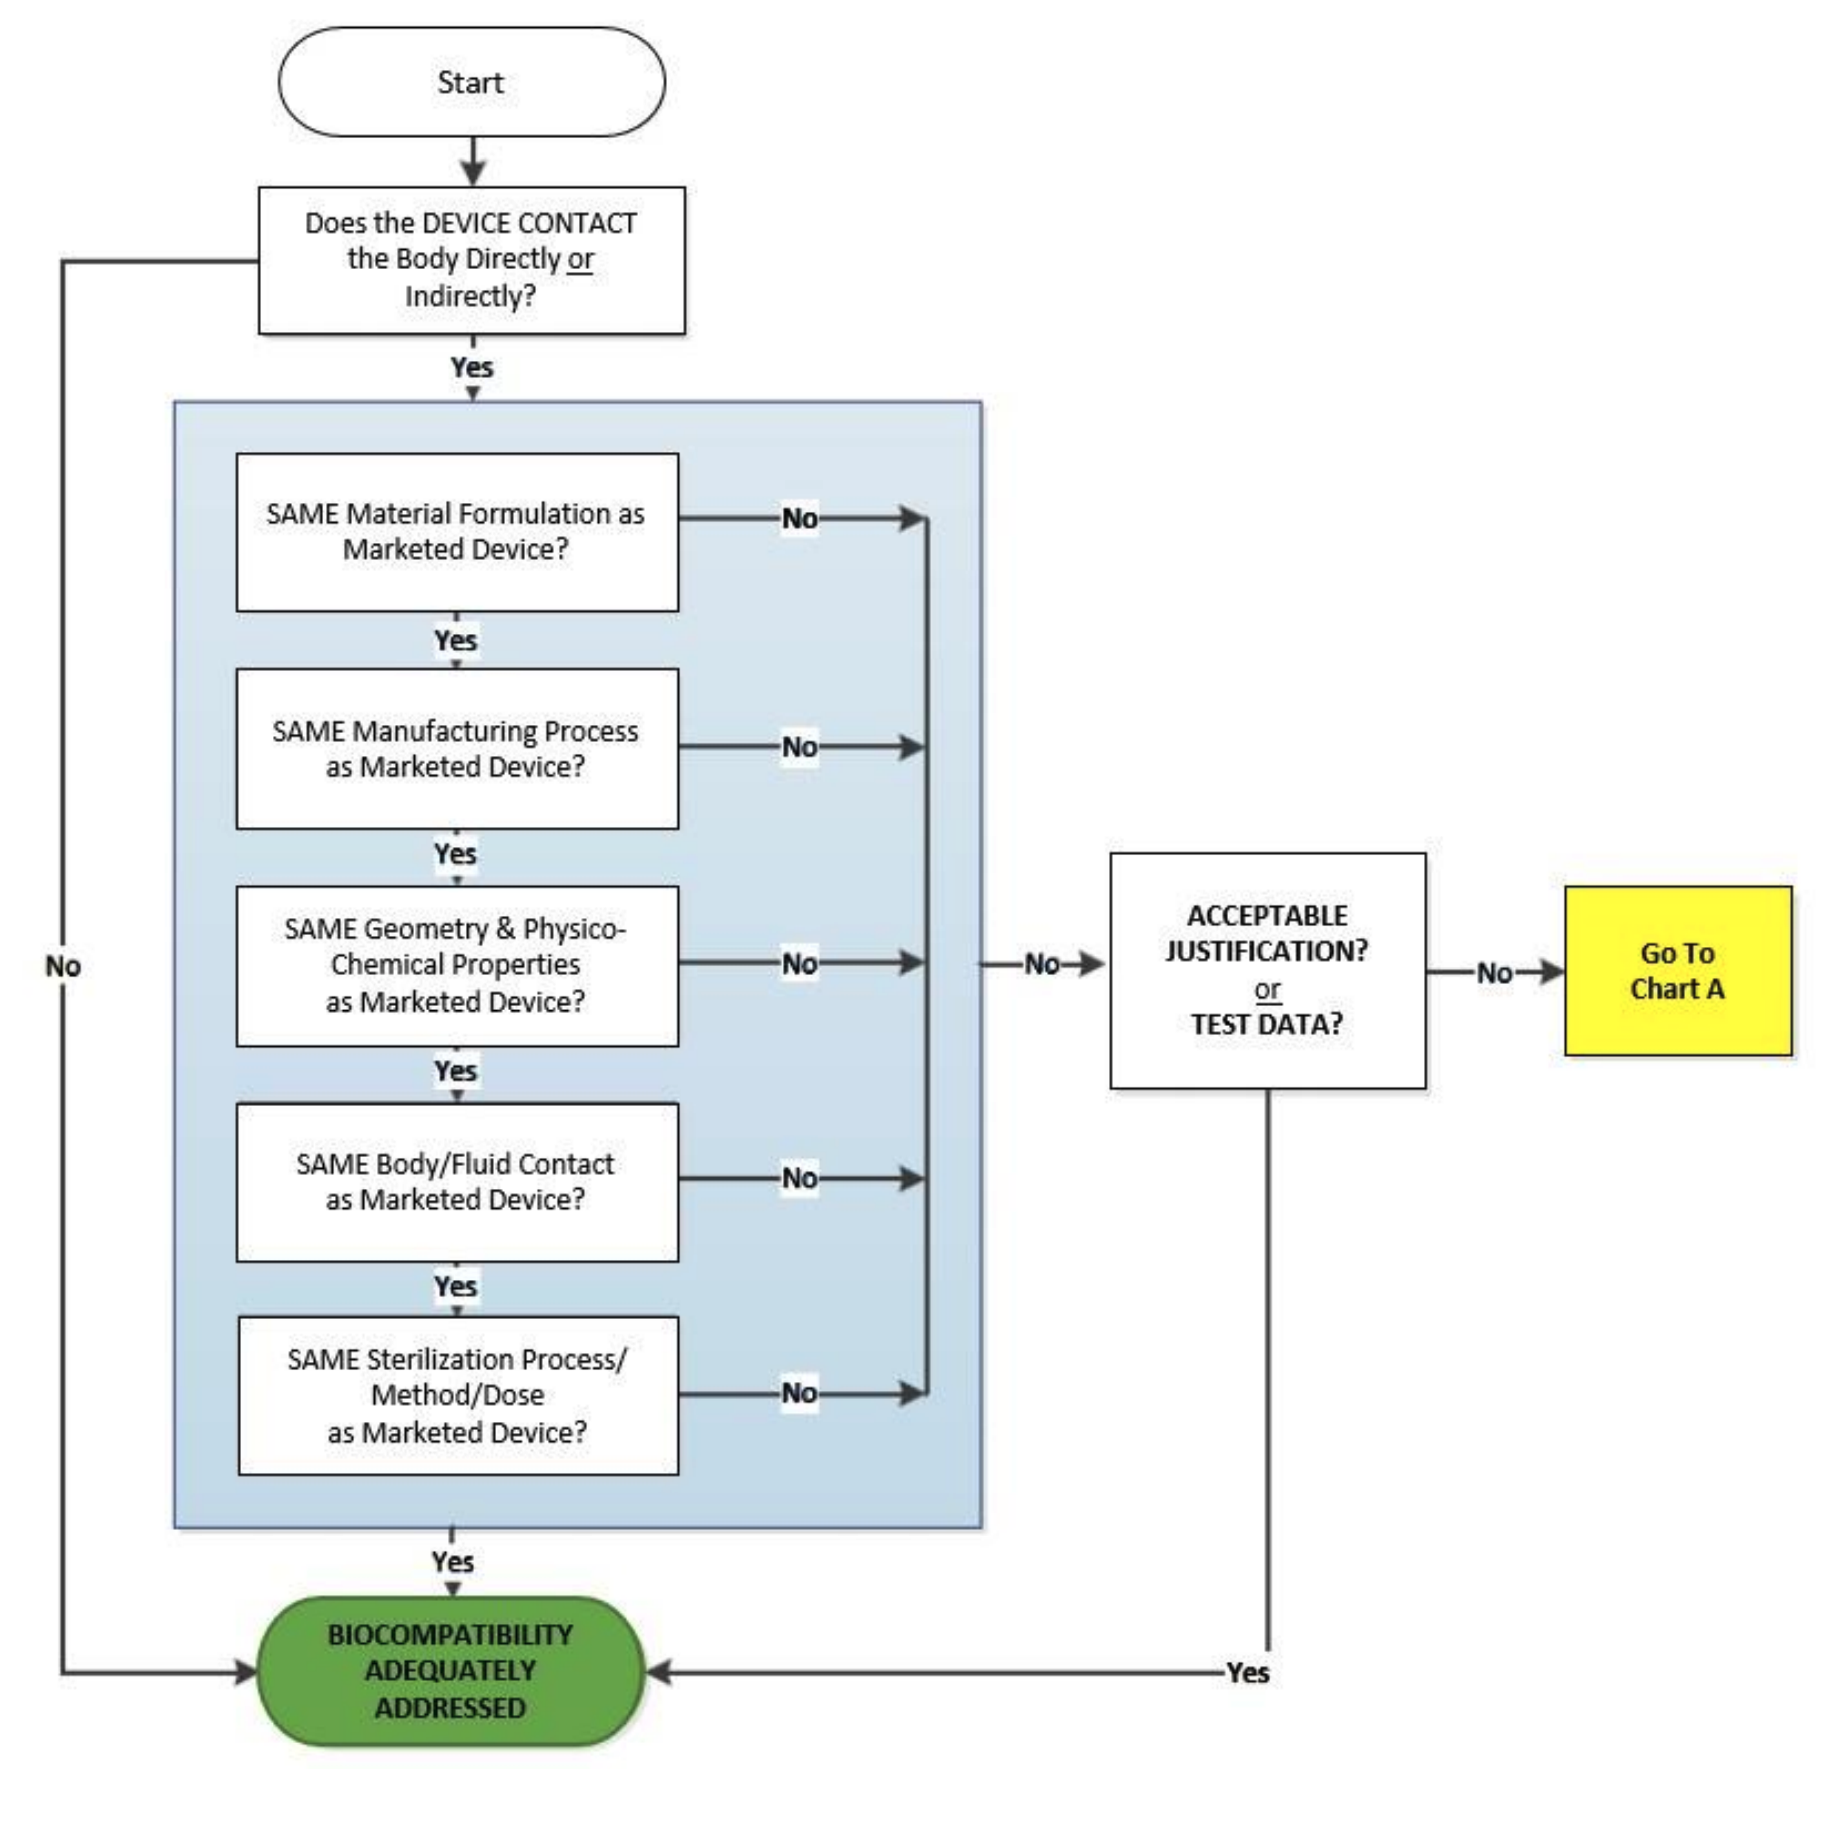
\includegraphics[scale=0.25]{figure1_fda.png}
	\centering
    \label{fda_1}
    \caption{main flowchart for biocompatibility evaluation in 10993-1:2018 standard \cite{healthUseInternationalStandard2023}}
\end{figure}
\begin{figure}[H]

	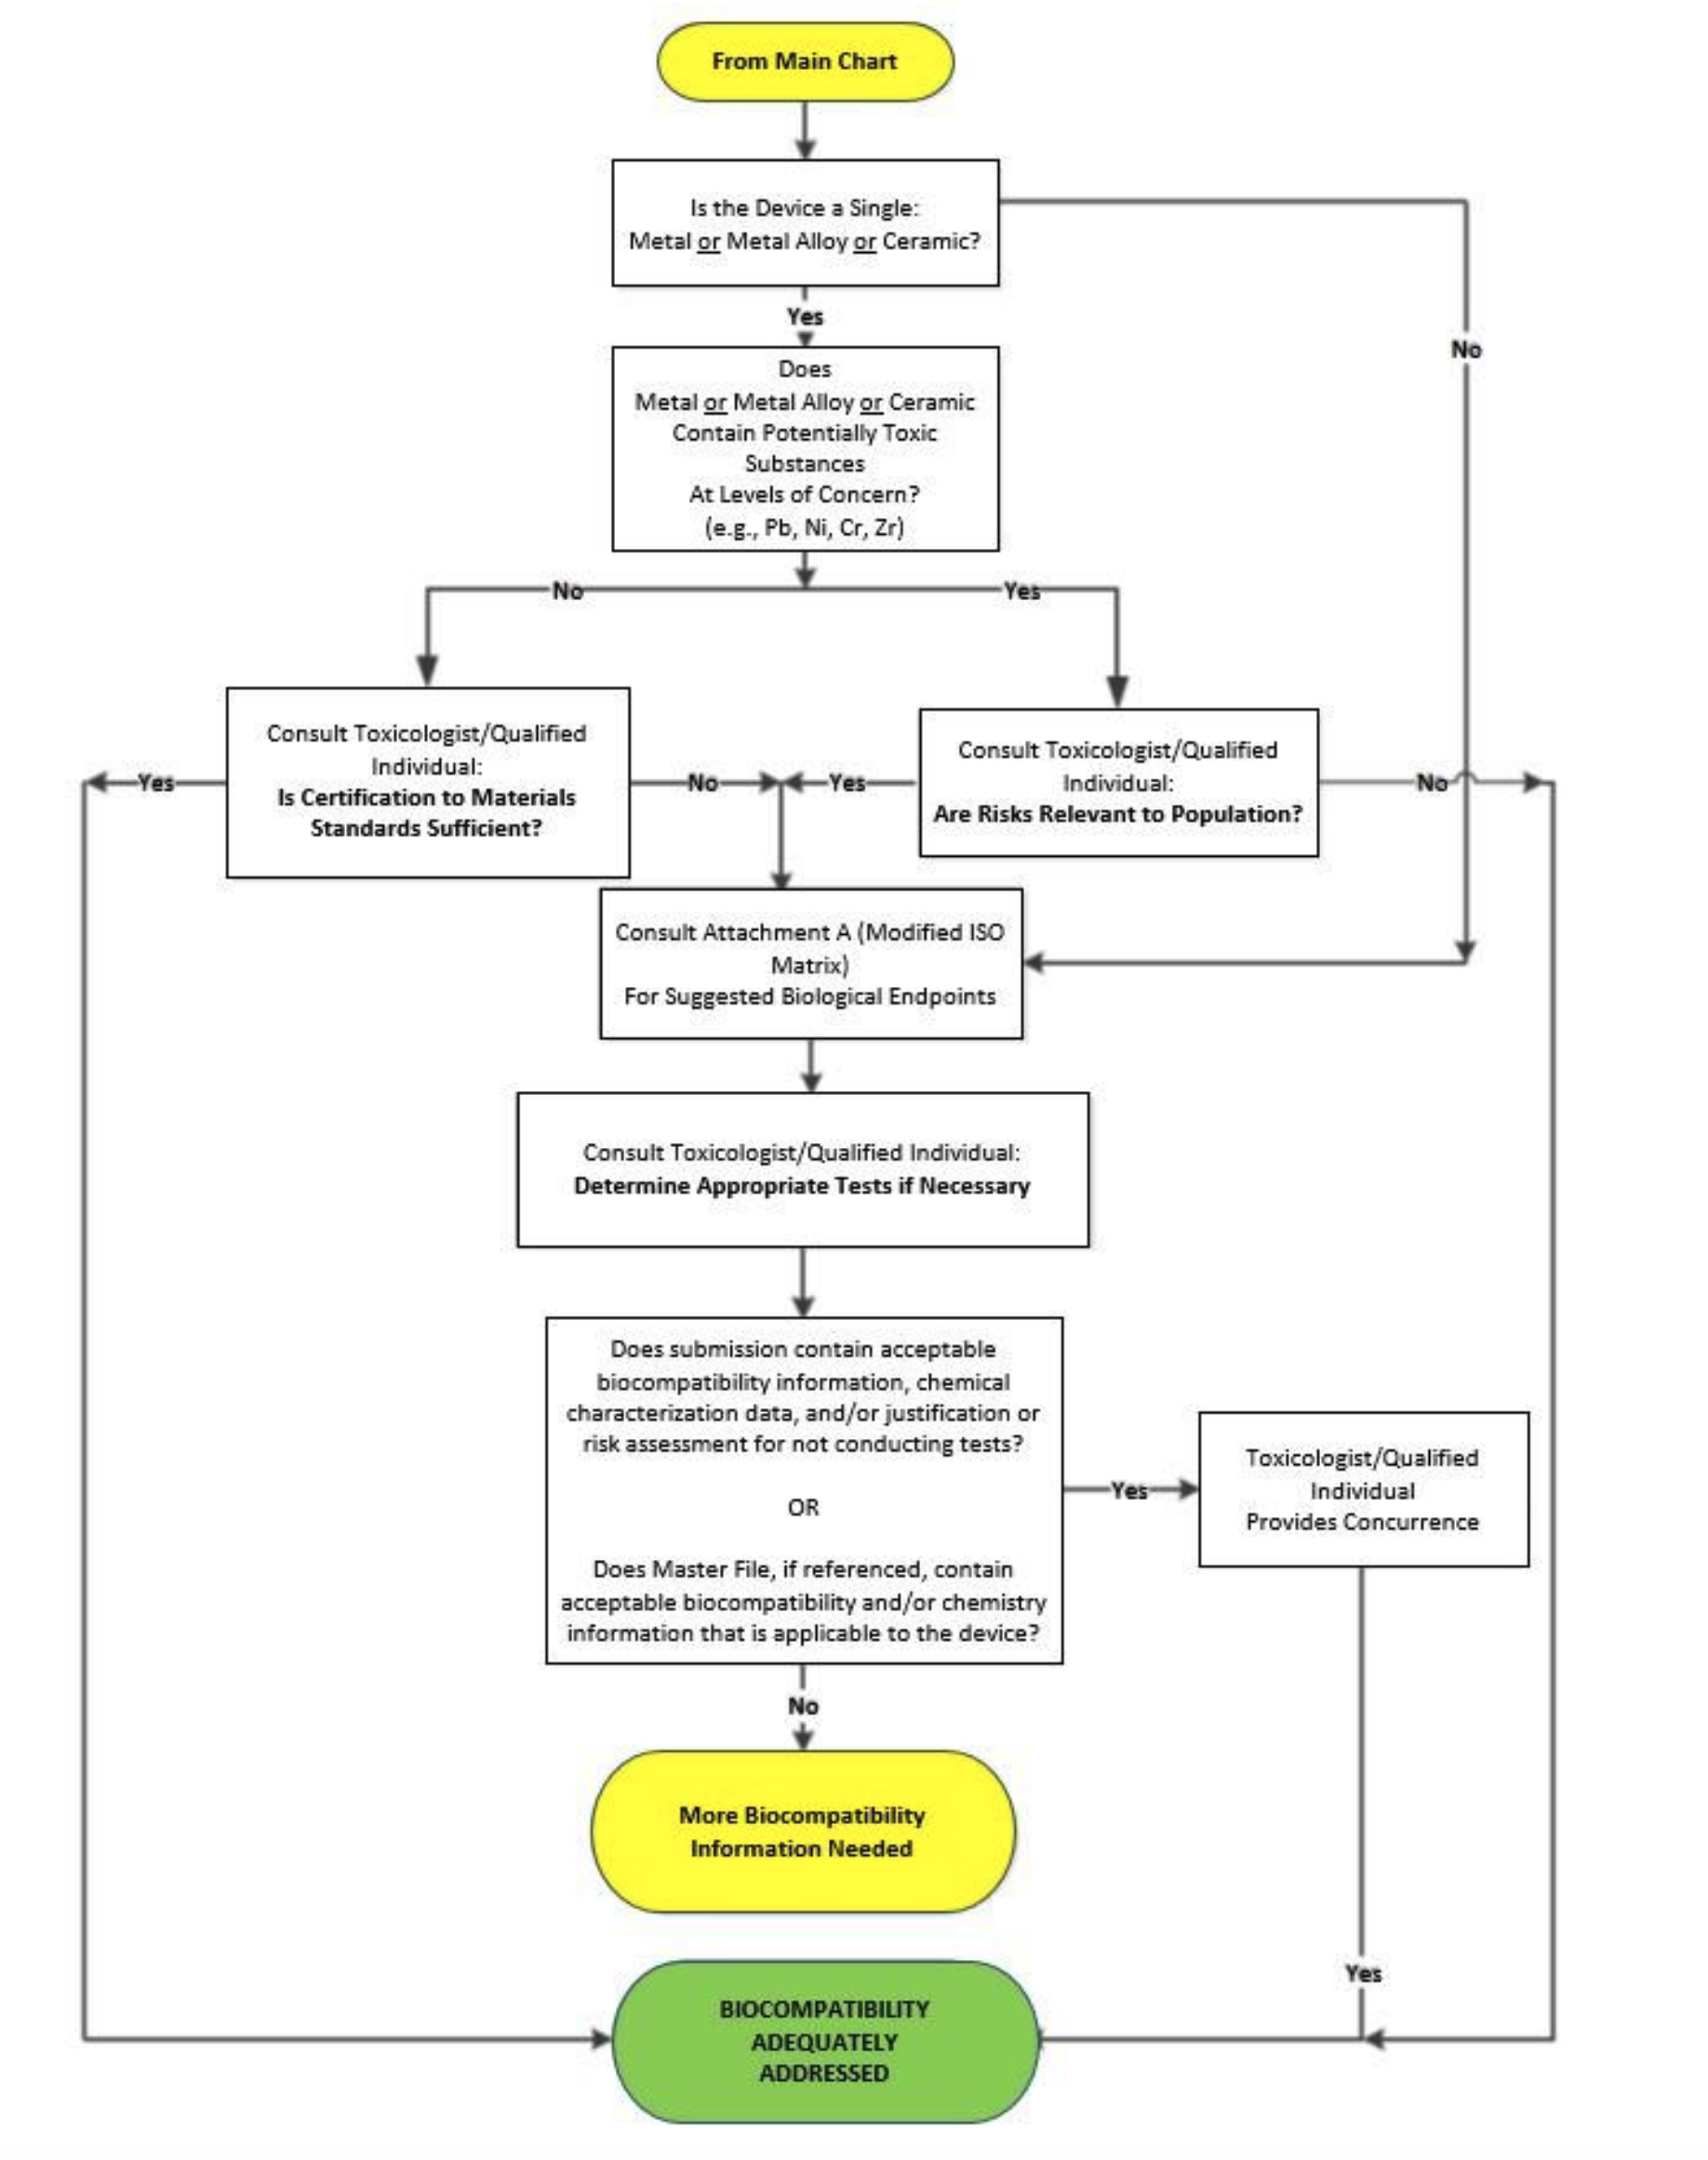
\includegraphics[scale=0.25]{figure2_fda.png}
	\centering
    \label{fda_2}
    \caption{CHART A for biomcompatibility evaluation in standard iso 10993-1:2018 \cite{healthUseInternationalStandard2023}}
\end{figure}


As it is possible to see from these flowcharts, biocompatibility evaluation is not necessary only if the device taken into consideration has not any direct or indirect contact with the body, or if it has the same properties of a similar well known device present in the market.
Moreover, devices are subdivided into three categories based on the nature of contact with the body: surface-contacting medical devices, which only have an external contact with the body such as the one in contact with the skin, externally communicating devices and implanted medical devices, which are again subdivided into their tissue of contact.

\begin{figure}[H]
	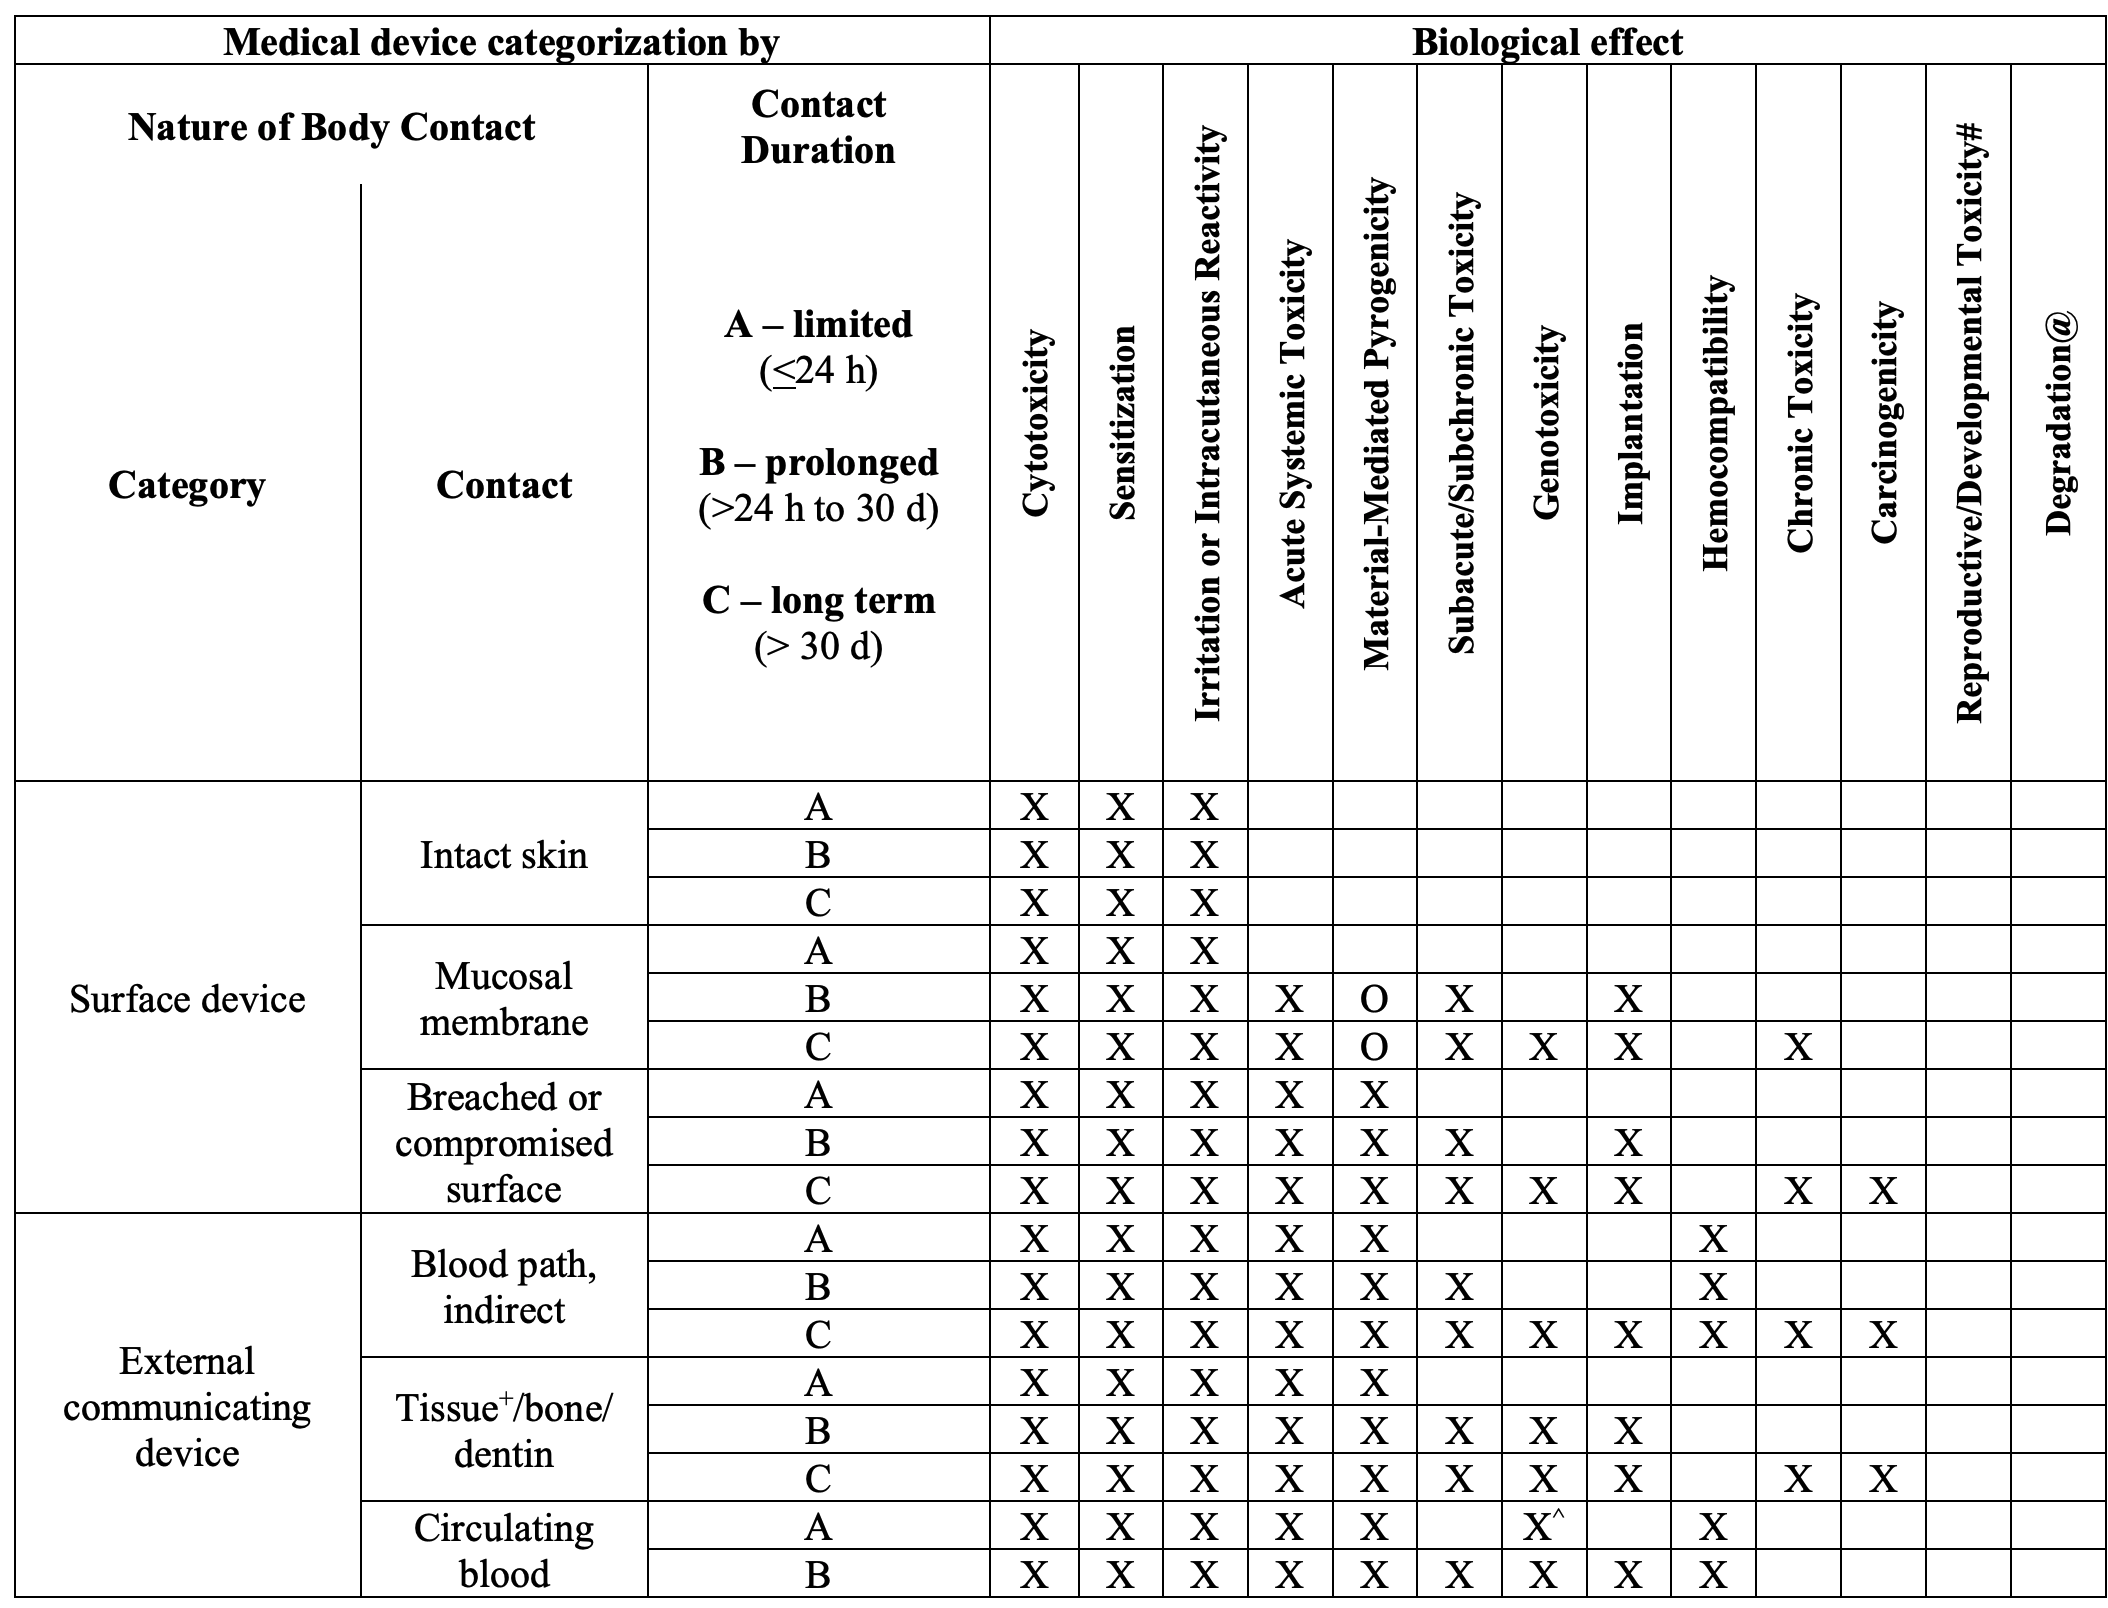
\includegraphics[scale=0.3]{tab1_fda.png}
	\centering
    \label{tab_da_1}
    \caption{Table A part 1 in FDA guidance \cite{healthUseInternationalStandard2023}, biocompatibility evaluation endpoints}
\end{figure}

\begin{figure}[H]

	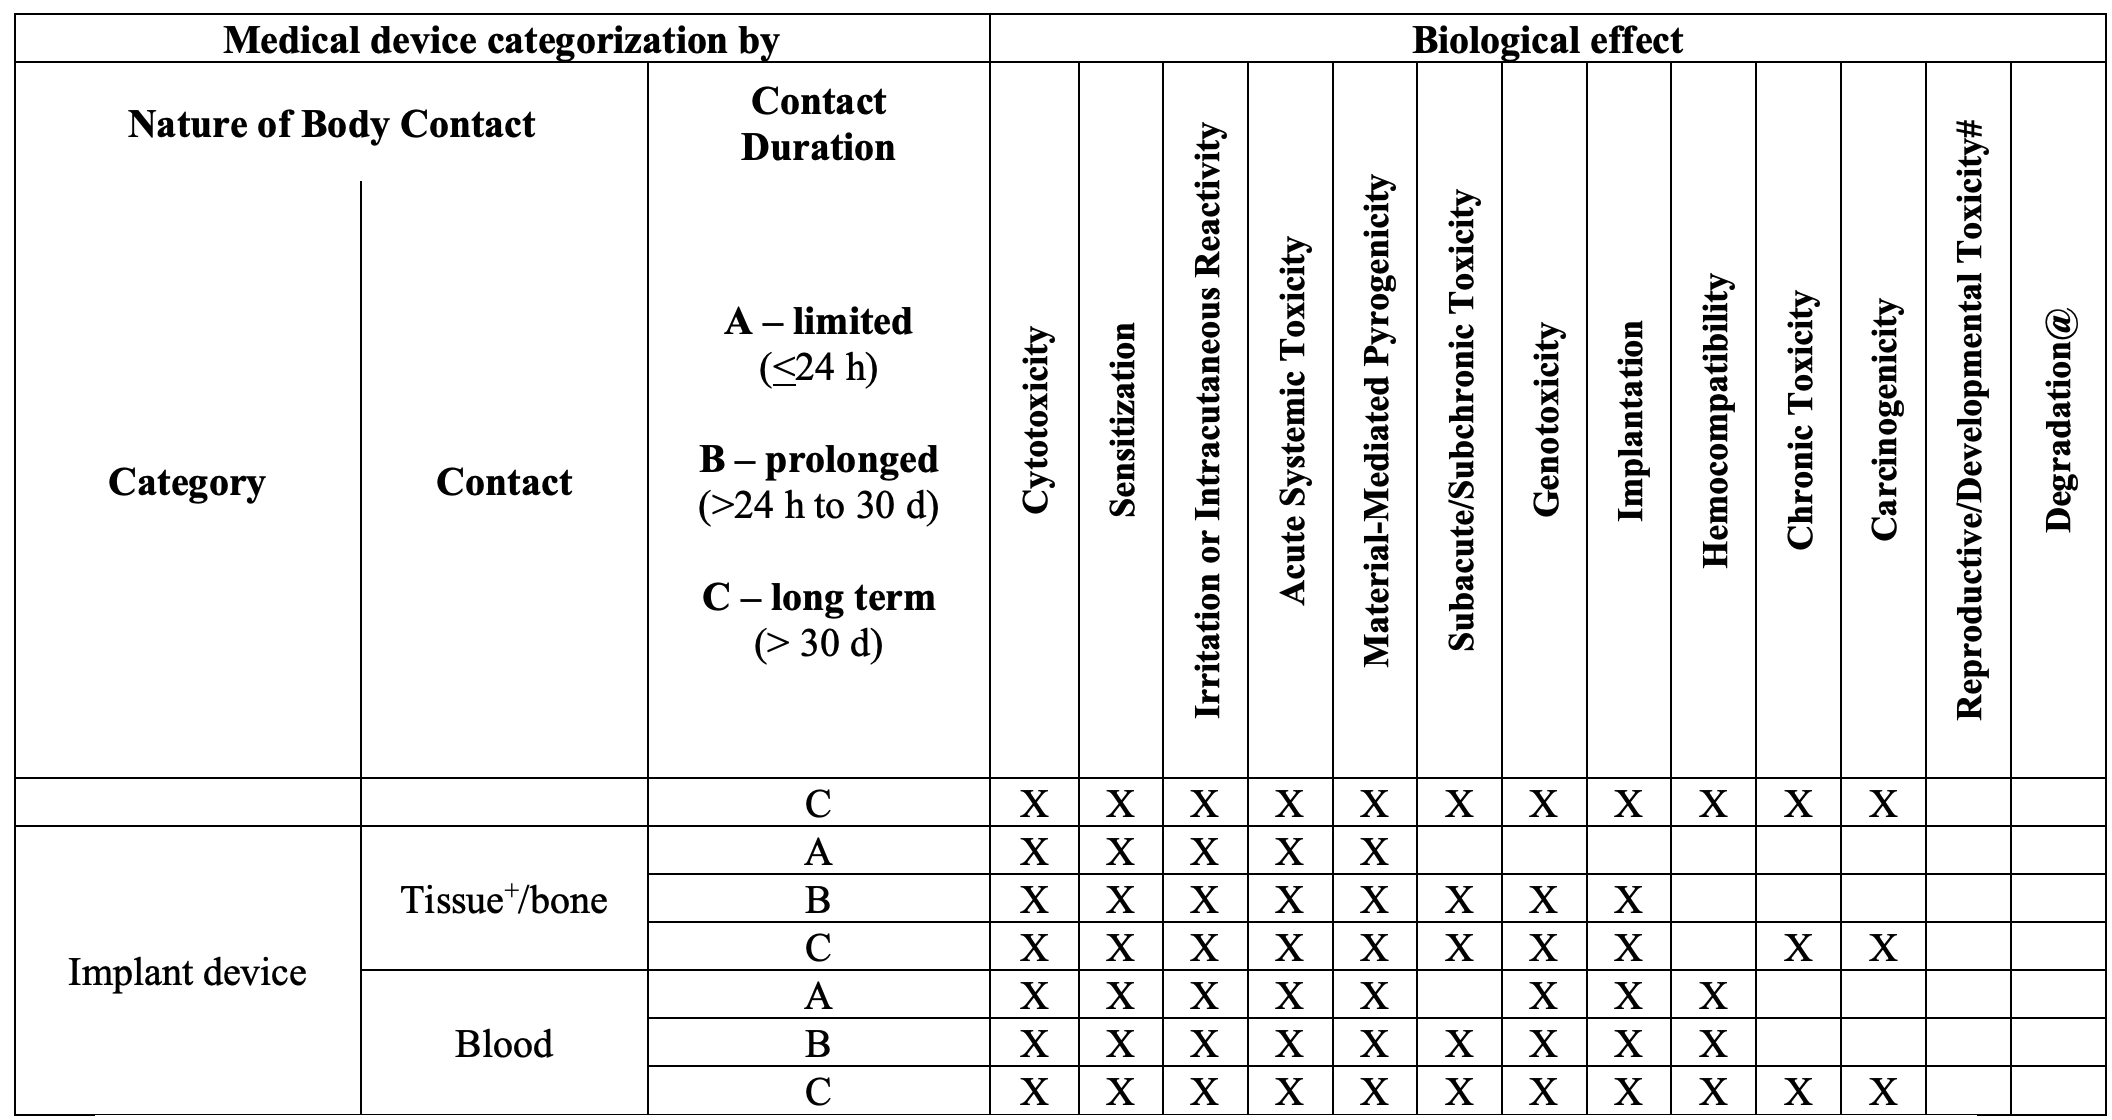
\includegraphics[scale=0.3]{tab2_fda.png}
	\centering
    \label{tab_da_2}
    \caption{Table A part 2 in FDA guidance \cite{healthUseInternationalStandard2023}, biocompatibility evaluation endpoints.}
\end{figure}

The table in Figure 2.3 and in Figure 2.4 shows, bases on the category of the product and the tissue and duration of contact, which could the possible biological effect that should be considered for the approval of the specific device.
Senseback could fall into the external communicating device category, with a long-term contact and tissue surface of contact, with relative biological effects reported in the table.  
FDA suggests that this table should not be threated as a checklist for testing. Instead, some specific medical devices the reported effects could not be enough and other endpoints should be considered.
For what concern cytotoxicity, the related ISO standard is 10993-5:2009 \cite{14:00-17:00ISO1099352009a}, a recent study \cite{gruberToxicNotToxic2023} has been conducted in order to verify whether this standard is clear enough to guarantee that devices development which have followed this standard are cytotoxicity safe. The conclusions report that different that this standard should be revised, because cytotoxicity tests performed by different companies with same standard cannot guarantee reliable and comparable results. This standard was last reviewed and confirmed in 2022. Therefore, this version remains current. 
UE regulations
In UE the normative that regulate the medical devices approval are the 2017/745/UE \cite{RegolamentoUE20172017} which is relative to medical devices and 2017/746/UE \cite{RegolamentoUE20172017a}, which is relative to in vitro diagnostic. The first one is applied since 26, May 2021, the second one since 26, May 2022 \cite{MedicalDevicesEuropean}. 
In these regulations, as before, devices are divided into classes of risks from the lowest, which is Class I to Class II-a and Class II-b to Class III, which is the highest one. The device classification follows similar step as in FDA evaluation, in fact some parameters are evaluated such as duration of contact, invasiveness, specific medical purpose and anatomical location \cite{PublicHealthEuropean2024} mcdg , it is up to the manufacturer to correctly classify the device according to the appropriate class of risk.
As reported in the regulations, all implanted medical devices and long-term surgically invasive devices are classified as class IIb \cite{PublicHealthEuropean2024} mcdg . However, since Senseback is an active device, which means that needs a source of energy which is different from the body itself, it could fall into class III, the highest one.
With the new normative UE 2023/607 \cite{RegolamentoUE20232023} the deadline for the manufacturers to adequate to 2017/745/UE and 2017/746/UE has been postponed based on the class of risk of the devices as shown in Figure 2.5

\begin{figure}[H]
	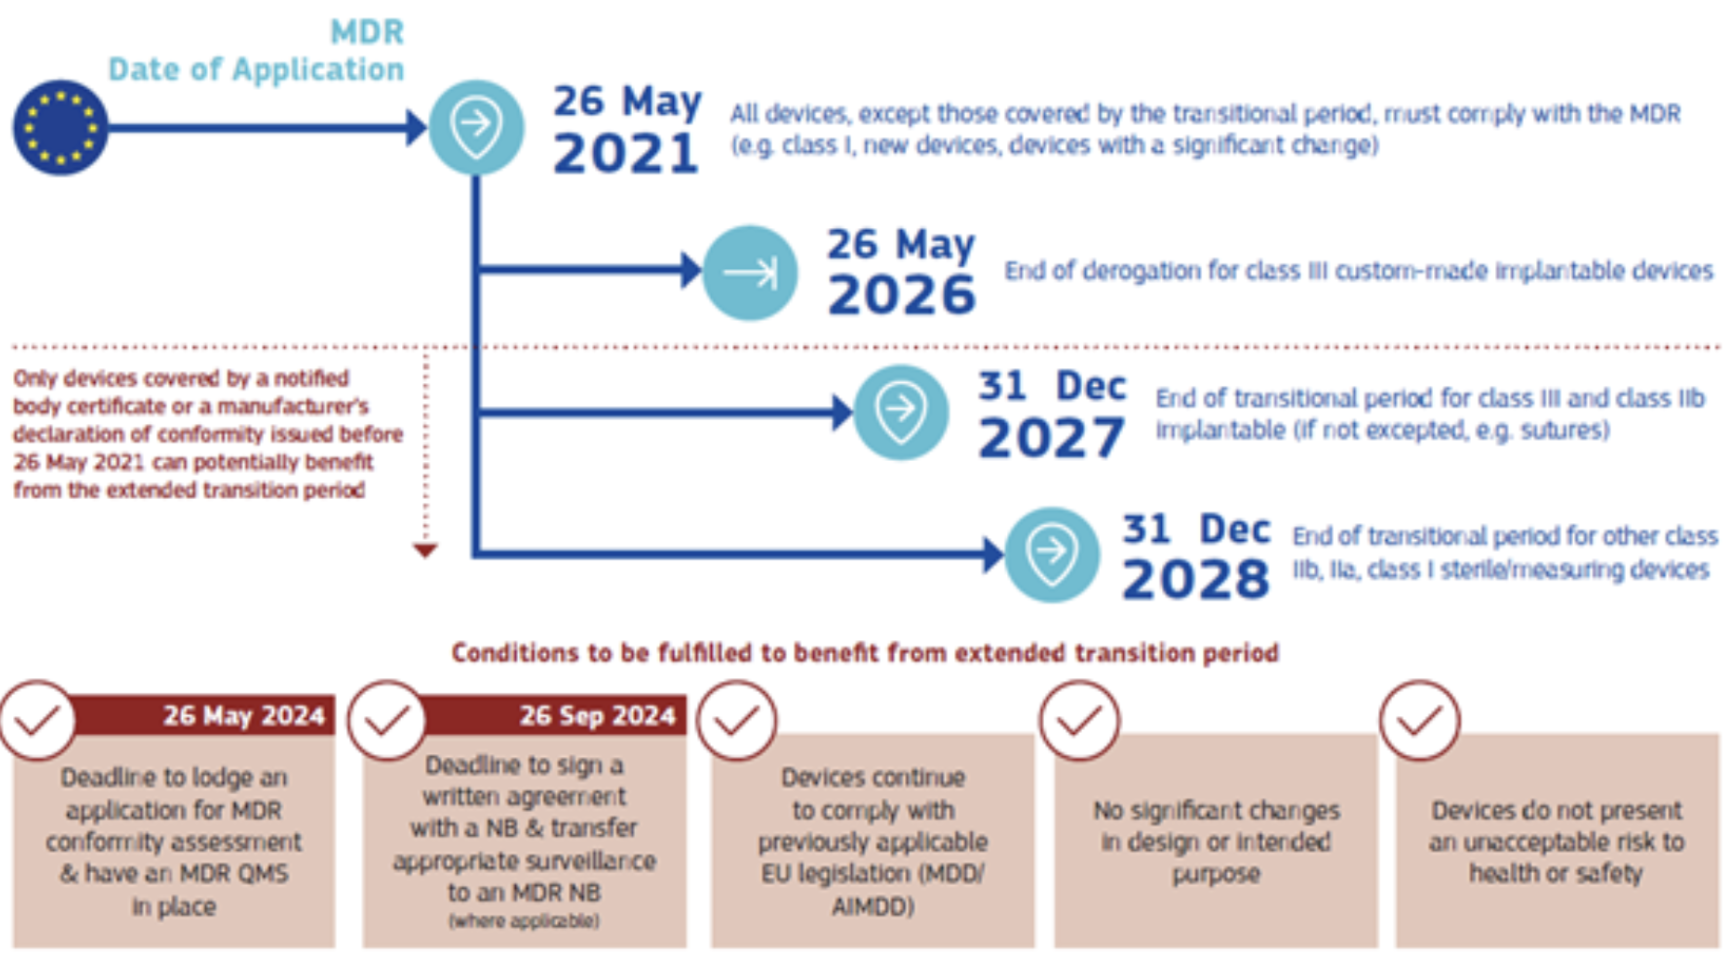
\includegraphics[scale=0.3]{Ethics/Screenshot 2024-08-15 at 10.54.56.png}
	\centering
    \label{ethics_1}
    \caption{new date of application of normative (EU) 2017/745 and (EU) 2017/746 according to (EU) 2023/607 \cite{NewRevisedResource}}
\end{figure}

\subsection{Medical software regulation}

According to the regulations EU 2017/745 \cite{RegolamentoUE20172017} and EU 2017/746 \cite{RegolamentoUE20172017a}, a medical software that is intended to be used alone or in combination with a hardware which fall under the definition of medical device should be considered as a medical device software (MDSW). 
In order to understand whether or not the software could be considered as a MDWS, the steps are reported in.

\begin{figure}[H]

	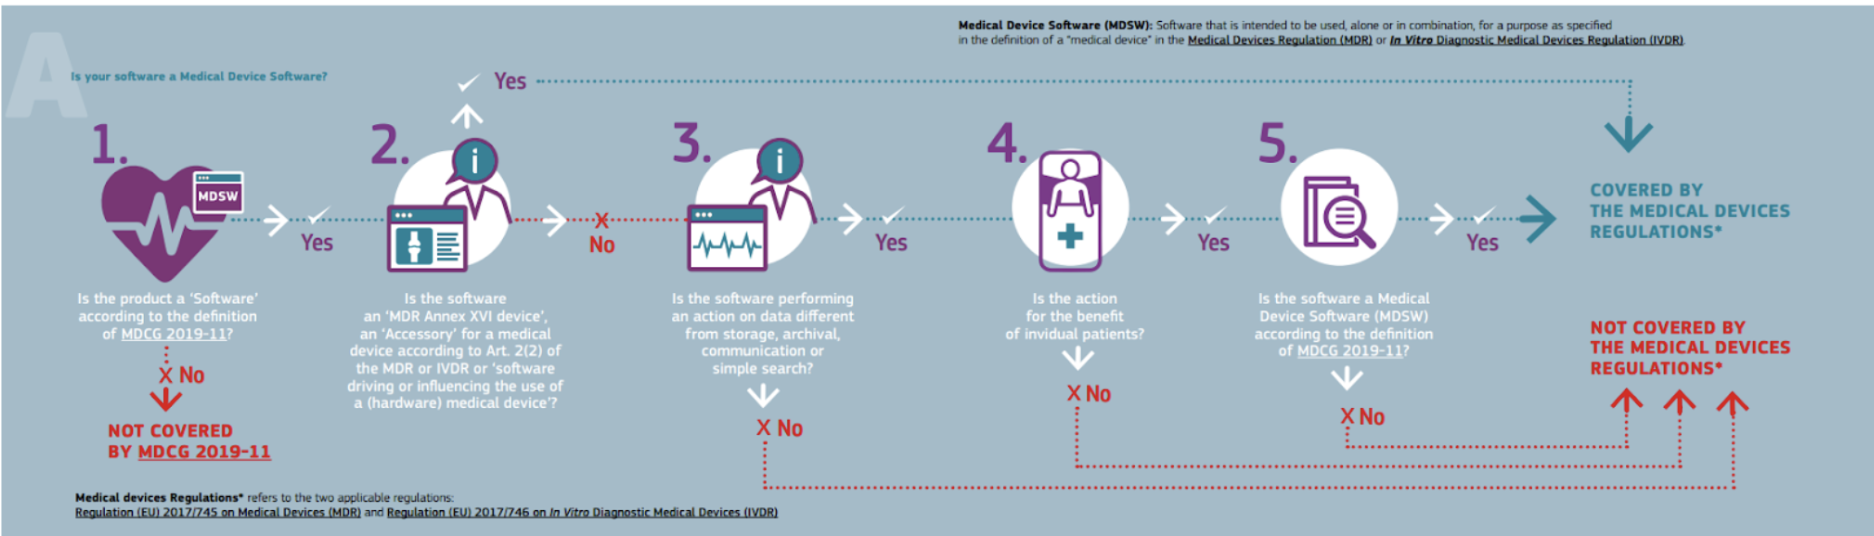
\includegraphics[scale=0.3]{Ethics/Screenshot 2024-08-15 at 10.55.04.png}
	\centering
    \label{ethics_2}
    \caption{Steps to verify whether or not the software falls into the MDSW definition according to European Commission \cite{PublicHealthEuropean2024}}
\end{figure}


First step is to verify that the software under analysis fall under the definition of software in the regulations, as reported in \cite{PublicHealthEuropean2024}, which states that “software” is defined as a set of instructions that processes input data and creates output data. Second step is to determine whether or not the software influences or drives the hardware device, if it does it could be classified as an accessory for the hardware medical device and as a consequence, be considered as a MDSW. If not, next steps need to verify which is the function for which the software is intended to be used, including whether or not the software provides an effective benefit to the patient. If it does and the software falls under the definition of MDSW in \cite{PublicHealthEuropean2024}, which states that a MDSW is a software that is intended to be used, alone or in combination, for a purpose as specified in the definition of a “medical device” in the medical devices regulation or in vitro diagnostic medical devices regulation, than the software should be treated as a medical device and it is covered by the new MDR regulations.
To sum up, a software is classified as a medical device if it satisfies the following characteristics: it should be independent, so it should have its own medical purpose, it can influence or drive the hardware medical device and it may be intended to be used by medical professionals. Note that a software can be classified ad a MDSW no matter the location intended for it.

The rules to classify a MDSW are reported in Annex VII \cite{massimopANNEXVIII2019}. As it is reported in chapter II, a software which is stand alone and has not influence on the hardware medical device should be classified separately. If it is not, however, it should be classified considering the most critical specified use. I the software and the hardware have two different classes of risks, as a consequence, they both fall into the highest class.

Senseback software, then, falls into the class of risk III. 

\subsection{Normatives for wireless devices}

In European Union, normative EU 2017/745 \cite{RegolamentoUE20172017} treat a wide range of medical devices, including the ones with a radio frequency communication such as Bluetooth low energy like the case in analysis. It is reported that manufacturers should ensure that devices are designed in a way so that external interferences such as external environment or radio signal interferences are removed or at least reduced as much as possible, so it is for possible undesired interaction with the environment which is thought for the device to be used with. 
In the United States, instead, FDA has provided a regulation \cite{healthWirelessMedicalDevices2023} which regards specifically radio frequency wireless medical devices, this is thought for all the devices which use at least one functionality with a wireless feature such as Bluetooth, WI-FI and so on. 
In this normative it is reported that wireless communication could be a benefit for the patient in terms of mobility, due to the fact that wires are not present anymore, moreover also a remote monitoring of the real-time health of the patient is possible. However, possible risks in patient daily life should be considered, and it is up to the manufacturer to inform the patient about them. Firstly, a possible issue regards the fact that airways are shared, and the device could be influenced by other devices operating the near range of work of the medical device which is intended to be used. The increasing usage of these kinds of products, including the non-medical one, could condition the medical device performance. The suggested aspects that the manufacturer should take into consideration are the following ones then:
Selection of the wireless technology 
\begin{itemize}

	\item Quality of service
	\item  Coexistence
	\item  Security
	\item  Electromagnetic Compatibility (EMC)

\end{itemize}
For these, many standards are directly suggested by FDA itself, such as the directives AAMI TIR 69 \cite{RecognizedConsensusStandards} or ANSI C63-27/D1.0 \cite{IEEEANSIC63} for what concern the Wireless coexistence or IEC 60601-1-2 \cite{IEC60601122014} for electromagnetic compatibility (EMC).
For the security field FDA issued a guidance \cite{healthCybersecurityMedicalDevices2023} on September 2023 which regards specifically the cybersecurity in Medical devices, this document substitute the previous one \cite{ContentPremarketSubmissions} issued on October 2014.


\subsection{FDA Medical devices cybersecurity }


According to FDA guidance \cite{healthCybersecurityMedicalDevices2023}, manufacturers have the responsibility of the identification of possible cybersecurity risks associated to their devices, including both the ones related to the device itself and the ones related to the environment in which the product operates, for example the ones introduced by device reliance on hospital networks.
FDA also recommends the submitting of a detailed documentation about the security features of the product which is intended to be approved by them. They also recommend that this information should take the form of views in order to effectively prove that the developed architectures are effective and safe. Manufacturers should demonstrate that security features are effectively been implemented and tested.
The necessary requirements asked by FDA are the following ones:
\begin{itemize}
	\item Authentication
	\item Authorization
	\item Cryptography 
	\item Code, Data and Execution Integrity
	\item Confidentiality
	\item Event Detection and Logging
	\item Resiliency and recovery
	\item Updatability and Patchability
\end{itemize}
Note that these aspects are just the suggested ones, but the necessary features may vary depending on the specific intended usage of the device.
These aspects are explained in detail in Appendix 1
\subsubsection{Authentication}
Authentication is divided into two controls: 
\begin{itemize}
	\item Authentication of information: this means that it is possible to prove that data are generated from a trusted and verified source and they have not been altered during the transmission to the endpoint.
	\item Authentication of entities: it is possible to prove the identity of an endpoint from which is the one which provides information.
\end{itemize}
The device then, needs to verify that information received from an external source are reliable and so are the ones generated from the device itself. 
Authenticity can then be evaluated for:
\begin{itemize}
	\item Information at rest (stored)
	\item Information in transit (transmitted)
	\item Entity authentication of communication endpoints 
	\item Software binaries
	\item Integrity of the execution state of currently running software 
	\item Any other appropriate parts of the medical device system where manufacturer’s threat model and/or risk analyses reveal the need for it
\end{itemize}
The effective strength of the authentication implemented is evaluated on the difficulty that an external unauthorised source would need to identify the decomposition of authentication scheme.
A cryptographic algorithm in general should be preferred, this is because non-cryptographic ones are generally weak. As a consequence, an attacker could easily emulate the behaviour of an authorized user.
Some of the other recommendations regards the usage of a proper authentication method such as the multi-factors ones, strong passwords choices, authentication requirement before possible software updates, anti-replay measure in communications which can result harmful and the avoidance of cyclic redundant checks as security control.
Furthermore, manufacturer should consider how the device reacts to a possible authentication failure.  
\subsubsection{Authorization} 
Authorization is required in order to prevent the access to sensitive information or resources. In a well-designed system, only an authorized which has fully permissions can have the access to specific functions of the medical device, depending of the least privilege principle. This means that, in case of a hacker attack, they should not be able to access to possible functionality reserved to the manufacturer in case they gained the credential associated to patient privilege.
The recommendation about authorization regards the access to the device, which should be limited to authorized users, the usage of timer in order to terminate sessions and “deny by default” principle, which means that device should reject unauthorized connections by default.
\subsubsection{Cryptography} 
About cryptography, this is suggested to be implemented because of its higher level of security. It is underlined that this should be properly implemented to avoid undesired vulnerabilities.
The recommendation which regards this field suggest the usage of industry-standard cryptographic algorithms, in particular the one suggested in the current NIST standard for cryptography, the algorithm should also allow the device to use the highest level of security possible, unless otherwise necessary. Recommendation also suggests avoiding a situation in which the fully revealing of the key for a specific device could implicate the revealing of keys for other devices. Eventually, it is suggested avoiding downgrades in security level unless they are strictly necessary for the health of the patient.
\subsubsection{Code, Data and Execution Integrity } 
Integrity is subdivided into three field: Code, Data and Execution. 
In the code field it is suggested, in addition to previous suggestions, to prefer, when possible, solution which are hardware-based, to disable the access to unauthorized ports such as the UART and to ensure that device is physically integer by employing the usage of tamper seals.
For data integrity, the suggestions regard the verification of the received data coming from an external source, which should be validated and not modified during the transit and the protection of the data which are relevant for the safeness of the device. 
Finally, for the execution integrity purposes it is suggested to use industry-accepted best practices to maintain the code integrity during the execution process and the design and review all code that handles external data.

\subsubsection{Confidentiality} 

Even if authentication ad authorization suggestions provided in previous points should be enough to ensure confidentiality, manufacturers should verify if for the specific implementation it could be necessary to implement additional features. A loss of confidential could result in a potential harmful effect on the patient.
\subsubsection{Event detection and logging} 
The suggestions regarding this point suggest that each security relevant event, in particular suspicious behaviours should be detected and logged promptly, including possible software changes or malfunctions. Manufacturers should also implement a log file in which these tracked events are stored. It is also suggested to design devices which are able to integrate antivirus/anti-malware protections.
\subsubsection{Resiliency and recovery} 
Resiliency and recovery are the capabilities of the device to face with a safety margin a possible incident scenario and maintain availability.
Manufacturers should then design devices which are resilient to possible incidents or noises, specifying the level of resilience that any component of the medical device have. Th design should also include methods for recovery default configurations and protections for critical functionality or data.
\subsubsection{Firmware and software updates} 
Last recommendations regard software and firmware updates. These should anticipate the future cybersecurity vulnerabilities, should be reliable even in case of interruption or failure of the process, and the cybersecurity related ones should be separated from regular feature update cycles. 
Moreover, it is indicated that updates should be easily verified, validated and distributed. Manufacturers should also implement all the necessary tools and processes to ensure that updates are applied in a safely ad timely manner. Lastly, third party licenses should be maintained for the whole life of the device.
\subsubsection{Cybersecurity regulations for medical devices in EU} 
Regarding cybersecurity, the European Union has recently issued the (EU) 2022/2555 \cite{DirectiveEU20222022} normative on Security of Networks and Information systems (NIS2), which is entered into force in January 2023. 
The normative is not just focused on medical device as the FDA guidance \cite{ContentPremarketSubmissions}, but it also discusses about them. The first article reports that the purpose of this normative is to establish rules in terms of cybersecurity risk management for the topics which are considered “critical” in normative 2022/2557 publicationsoffice or the ones reported in the Annex I or Annex II of (EU) 2022/2555, such as point 5.a of Annex II which is referred to the fabrication of medical devices and diagnostic medical devices in vitro. 
In NIS2 a distinction had been made between important entities and essential ones, allowing to have in this way a fair trade-off between risks-based requirements and relative obligations and administrative burden stemming. As it is reported in Article 3, entities in Annex II could be classified as essential depending on whether or not they are classified like that by a Member State.
One of the main differences in terms of regulations between important entities and essential entities is the fact that the essential ones are proactively supervised by the authorities, while important ones are subject just to a light ex post supervisory regime, which can be triggered in cases in which evidence of a possible infringement of the directives are brought to the authorities.
In the article 21 point 2 of the NIS2 directive cybersecurity management measures are threated, which both essential and important entities should follow. It is reported that companies have to manage their own security risks and take adequate measures to manage them. 
The recommendations about the measures to take are reported below. They need to include:
\begin{itemize}
	\item Policies on risk analysis and information system security 
	\item Incident handling
	\item Business continuity and crisis management
	\item Supply chain security
	\item Security in network and system acquisition
	\item Policies and procedures to assess the effectiveness of cybersecurity risk management measures
	\item Cryptography and encryption, and multi-factor authentication
	\item Cybersecurity training and basic cyber hygiene practices
\end{itemize}



\section{Ethical concerns}

Even if scientific and biomedical research is essential for the development of our society, it helps people to recover from medical diseases which were chronical before for example, it is important to wonder which is the limit that medical research should reach.
Ethical implications should then be considered, especially in some setups like the one considered in this Master Thesis, which purpose is to have in close future an effective usage in vivo.
In all of the steps, from the premarket ones and relative experimentations to the post market ones and relative surveillance, ethic should be taken as a monitor, in order to guarantee that not only the device in use is safe and effective, but also the development of it has been made respecting environment, the work ethic of people involved in, and the eventual animals used for the experimentation phase. To do that, research should be the as transparent as possible, by clearly explaining the goals and the intended benefits of the project, the methods and design of the study and which could be the possible risks. 
When available the results of the study should be published, possibly even the experimental ones. This would contribute to the check of the results by other researchers, promoting the re-doability and consenting a critical evaluation of the work. In case of possible criticisms or questions coming from the scientific community, these should be answered, and corrective actions should be taken when necessary. The practicality of sharing the information on the project is essential in an ethical and responsible research. 
Some of the principal ethical topics that should be considered in the context of PNrelay project are treated in detail below.


\subsection{Animal welfare }

The first aspect that should be considered for this purpose is animal welfare. The World Organisation for Animal Health (OIE), defined animal welfare as follows: An animal is in a good state of welfare, if it is healthy, comfortable, well-nourished, safe, able to express innate behaviour, and if it is not suffering from unpleasant states such as pain, fear and distress \cite{Chapter}. Animal welfare, in this kind of research, implies the careful and responsible consideration of the management, the treatment and health conditions of the animals involved in the research.
Animals are still necessary to test pharmaceutical or medical products before putting them into the market, because the experimental phase made on animals guarantees that each product on the market is effectively safe and which could be eventual collateral effects that patients should be warned about. However, the treatment of the animals involved in the experiments must be ethically correct. This means that this phase should respect current rules and animal welfare regulations, and this also means that animal experimentation is made only when necessary and the least number of animals is involved. 
The Animal Welfare Act (AWA)  \cite{AnimalWelfareEU} comps was the first policy responsible for guaranteeing the standards for animal welfare in the USA. It included rules relative to transportation, treatment during tests and research, teaching and dealings by animal dealers. This standard was issued in 1966, but it only covered some warm-blooded animals such as dogs, cats or rabbits, and some other animals like birds or rats, which are the ones mostly used in scientific experiments, were excluded from the act. The Act was amended eight times until now, however it is just in 2002 with the publication of Farm Security and Rural Investment Act \cite{CongressgovLibraryCongress} plaw that the excluded animals, including rats used in medical research, has been included into the definition of “animals” of the Animal Welfare Act.
The European Union also issued some policies to define the minimum standards necessary for animal welfare, which are some of the world’s highest animal welfare standards \cite{AnimalWelfareEU}. The current normative responsible for setting this kind of standards in the EU is the 2010/63/EU \cite{Direttiva201063}, published in 2010 and effective 1 January 2013. It is strictly related to animals used for scientific research and treats all the related steps, from development to manufacture to tests. The ultimate goal would be to have fully non-animal methods.
By following these policies and by implementing the right measurements to guarantee animals well-being, it is possible to reduce the negative impact on the life of the animals involved in the study.
Some of the terms that implies a sufficient welfare of the animal are:
Implant procedure. The chirurgical procedure necessary for the implanting of the device should be painless and as less invasive as possible. It is important to reduce at the minimum the pain of the patient during this operation and guarantee that the patient would have sufficient time for recovery after that. 
Health monitoring. The health of the patient should be monitored for the whole time of the experiment. This includes the monitoring of vital functions, the behaviour of the animal and physiologic indicators.
Duration of the experiment. The experiment duration should have the strictly necessary duration to get the necessary data for the experiment. The minimum number possible of involved animals should also be considered.
Usage of positive and negative controls. They should be implemented in order to check if the observed effects are due to the intervention or external environment.
Environment in which animals live. This should guarantee that animals' physiological needs are respected. These include water and food access other than movement range and social iteration.
Biological behaviour of the animals. The natural behaviour of the animal involved in the experiment should be respected, including the possible negative impacts on their daily life, which should be minimised.
In those cases in which euthanasia is necessary, it should be performed in agreement with the current normative of the corresponding country. This process should be conducted in a way which is ethical and respectful towards animals, making sure that this is conducted with attention on animal welfare. 
When possible, animal usage should be avoided in favour of cultured cells and computer-based models.
Transparency. The documentation of all the precautions taken during the study underlines the ethical diligence of the research.





\subsection{Need of research}


When approaching biomedical research, in which living beings are involved, it should be considered whether or not the intended research is necessary and whether or not the purpose of the research could be reached without animal usage. It is important for this purpose to make a trade-off between the possible benefits that people or animals could get from the research and the eventual damages caused to animals. 
The concept of “Need” for research refers to whether or not there is proper justification and needs to conduct the intended research. This means that developers should wonder whether or not the research faces a significant demand in the scientific development and in practical applications, these could justify resources usage and experimentations conducted on the animals.
In order to make sure that ethical implications have correctly been monitored in the intended experiment, it is suggested to submit it to a careful revision from an ethical committee or institutional ones. 
To sum up, needs of the research means carefully wondering about the scientific and ethical value of the project, making sure that these justify animal involvement. These precautions make sure that research is conducted in a responsible way and it is in line with the highest ethical standards.

\subsection{Safeness of the patient}


The concept of safety of the patient is fundamental for guaranteeing that the iteration between the device implanted in the animal’s body and the external device happens in a safe way and it does not involve any risks for the animal's health.
One of the first aspects that should be considered for this purpose, is the fact that materials should be safe and biocompatible. The utilised components should minimise risks and adverse reactions in surrounding tissues. A careful planning and a correct post-operation management could contribute to reducing the minimum uneasiness and collateral effects.
Moreover, during the implantation procedure, protocols should be adopted in order to prevent possible risks of infections. Hygiene is essential to prevent issues that could intact the safety of the animal.
Furthermore, considering that Senseback communicates with the external device wirelessly, the right procedures for assuring that the protocol of communication, in this case for Bluetooth Low Energy (BLE), is secure and cryptographed in order to protect sensitive data. This is essential for the protection of the privacy of the patient.
Lastly, it is important to consider the procedure to follow in those cases in which the experiment presents issues or complications. This includes the planning of emergency procedures and the possibility to interrupt the experiment if some warnings related to the safety of the patient come up.

\subsection{Inclusivity}
 

The concepts of inclusivity and heterogeneity are linked to ethical and social considerations related to equal access, representation and to the individual differences in the process of research and in the application of the results.
Firstly, the project should promote equality in the access of the benefits coming from the research. This includes the consideration on how the application of the technology can be made available to different ethnic groups, avoiding discriminations and differences in the therapeutic approach.
Talking about this specific project, this is intended to be experimented on animals in next few years, however in a distant future this should be made available on humans. For this reason, the differences between the group of patients should be taken into consideration, to make the project more general and inclusive. An example of this is a study, \cite{nagaokaDevelopmentRealisticHighresolution2004} proposed by Institute of Physic and Engineering in Medicine (IPEM), in which a whole-body voxel model for the average Japanese man and woman has been developed. This study shows how different are some physical effects such as SAR on the body. A comparison with previous studies, in which only Caucasian men were studied, has been performed in order to underline the differences. This study should be taken as a monitor to take into account that different bodies of men and women of different ethnicities could have some substantial differences. Moreover, the project should also respect individual differences in response to technology in order to maximise efficiency and minimise collateral effect. Some genetic, physiologic or lifestyle related variations or possible disabilities can influence the response of the patient to the treatment. The project should then be relatable for the higher range of individuals possible, including the ones with special needs. Furthermore, the manufacturer should also consider how the related project could impact society in terms of inclusion and diversity and which could be possible positive or negative effects on social dynamics and equity of health.
Inclusivity could also mean the respect for different cultural sensitivities, which should be taken into account in the design of the project. Medical practices could vary by varying the country and these differences must be considered. Research could work in strict contact with the related community, this could help to better understand the needs and the expectation of the people involved.
Also the informed agreement in case of experimentation on humans should be sensitive to culture and should be understandable for all the participants. Information contained in that should respect differences in terms of language and culture.
All in all, the concepts of inclusivity and diversity focused on the obtaining of an equal approach, representative and respectful of the differences both in the research phase and in the usage one. The attention to these considerations would contribute to guarantee that the project has a positive impact on a larger range of individuals and communities.


\subsection{Informed agreement }

Informed agreement is crucial in those projects in which humans are involved in experimental research or in the application of new medical technologies. The informed agreement is an ethical process which guarantees that all the participants have a complete view of the intended purposes, the risks and the possible benefits of the research or the medical intervention in which they have given their voluntary consent to participate. Before submitting anyone to experimental treatments or to procedures linked to the related technology, it is necessary to get an informed agreement.
In the agreement it is important to furnish to the participants all the necessary details about the procedure, including the goals of the study, the kind of intervention that will be made and possible issues or risks. All of the available options should be illustrated, and information about possible alternative or standard treatments. This allows participants to make clear decisions about their participation. 
The agreement should also assure that anyone who is not purported to participate anymore could retire themselves from the study without any negative consequence. This enforces the principle of voluntary consent and respect about the autonomous decision of the participant.
The operator should explain in detail and in a clear manner how technology will work in the context of treatment or research. The participants should have the chance to ask questions and receive clarifications about the utilised technology.
For what concerns animals, since they cannot give a proper informed agreement, it becomes more and more important to have a consent from an ethical committee and from authorities. This will assure that animal welfare is respected.
Ultimately, researchers should have a clear documentation of the informed agreement, including the details related to the explanation given, the comprehension from the participants and their signs. This documentation is fundamental for transparency and ethical conformity.
To conclude, assuring that an informed agreement is obtained in a complete and ethical manner is fundamental for the respect of rights and dignity of the human or animals participants involved in the project.

\subsection{Privacy and surveillance}


Considering that in the Senseback project a wireless communication (BLE) is used, the concepts of surveillance and privacy are fundamentals and should be treated.
It is essential that, in the communication, security regarding the transmission of data is guaranteed. To do that, all the necessary robust precautions, such as cryptography, should be taken, in order to protect the communications from possible non authorised interceptions. It is also important to focus on the nature of the transmitted data, only necessary information should be shared, and the communication should be limited to the finalities related to the project.
Due to the sensitive nature of the biological or medical information, the privacy of the generated data should also be protected. To do that, measures to guarantee that data are treated in accordance with privacy-related laws and ethical standards becomes crucial. Moreover, collected data should be conserved and stored in a secure way, by limiting the access just to necessary cases and by implementing security protocols to avoid losses, manipulations and unauthorised accesses.
Another precautions to guarantee the privacy of the patient is the anonymity of the data when possible, especially in those cases in which data are shared or aggregated. This would protect the identity of the patient involved in the project.
Other than communication, also the device in usage should be securely designed. This includes protections against unauthorised access to the device itself and preventions against possible risks linked to the implant.
In addition, during the informed agreement, human participants should be warned about data management and privacy. They should have a clear explanation about how their personal information will be treated and an explicit agreement about storage and usage of data should be furnished. In particular, it is important to follow the norms related to the privacy of the patient in the related geographical context, in order to guarantee that the project is ethically and legally acceptable. In EU privacy is regulated by the General Data Protection Regulation (GDPR) \cite{L_2016119EN01000101Xml}, whose publication has provided a clear regulation for personal data treatment. In the USA, privacy regulation is not uniform and it is present just in some states like in California with the California Consumer Privacy Act (CCPA) \cite{californiaCaliforniaPrivacyProtection} california or in Virginia with the Virginia Consumer Data Protection Act (VCDP) \cite{CodeVirginiaCode}. Normative however, should be continuously monitored, since dynamics related to privacy can evolve and the adaptation to new normative or to the recent ethical worries is essential.
To sum up, the concepts of surveillance and privacy regard the responsible management of sensitive information, while it is guaranteed that secure measurements are in line with the ethical and legal normative applicable. This is fundamental to respect the rights and dignity of the involved people and to maintain trust in the research. 




\chapter{State of the Art}

\section{Bluetooth Low Energy Introduction}

Bluetooth is one of the main widely used wireless systems of communication. It is especially used in devices, such as headphones, which can easily be recharged without complications. However, this is not the case for applications such as microcontrollers, where the recharging process is not so immediate and high-speed communication is unnecessary. 

Because of this Bluetooth version 4.0, Bluetooth Low Energy (BLE) has been introduced. Using Bluetooth Low Energy instead of Bluetooth means sacrificing some amount of communication speed to save power consumption. The data rate reduction is achieved through two modifications: firstly, the payload in each packet is reduced from 1021 bytes in standard Bluetooth to 255 bytes in BLE. Secondly, data is sent as infrequently as possible to minimize the connection time, which significantly impacts power consumption. The main characteristics of BLE are shown in Figure~\ref{ble_char}.

\begin{figure}[h]
    \centering
    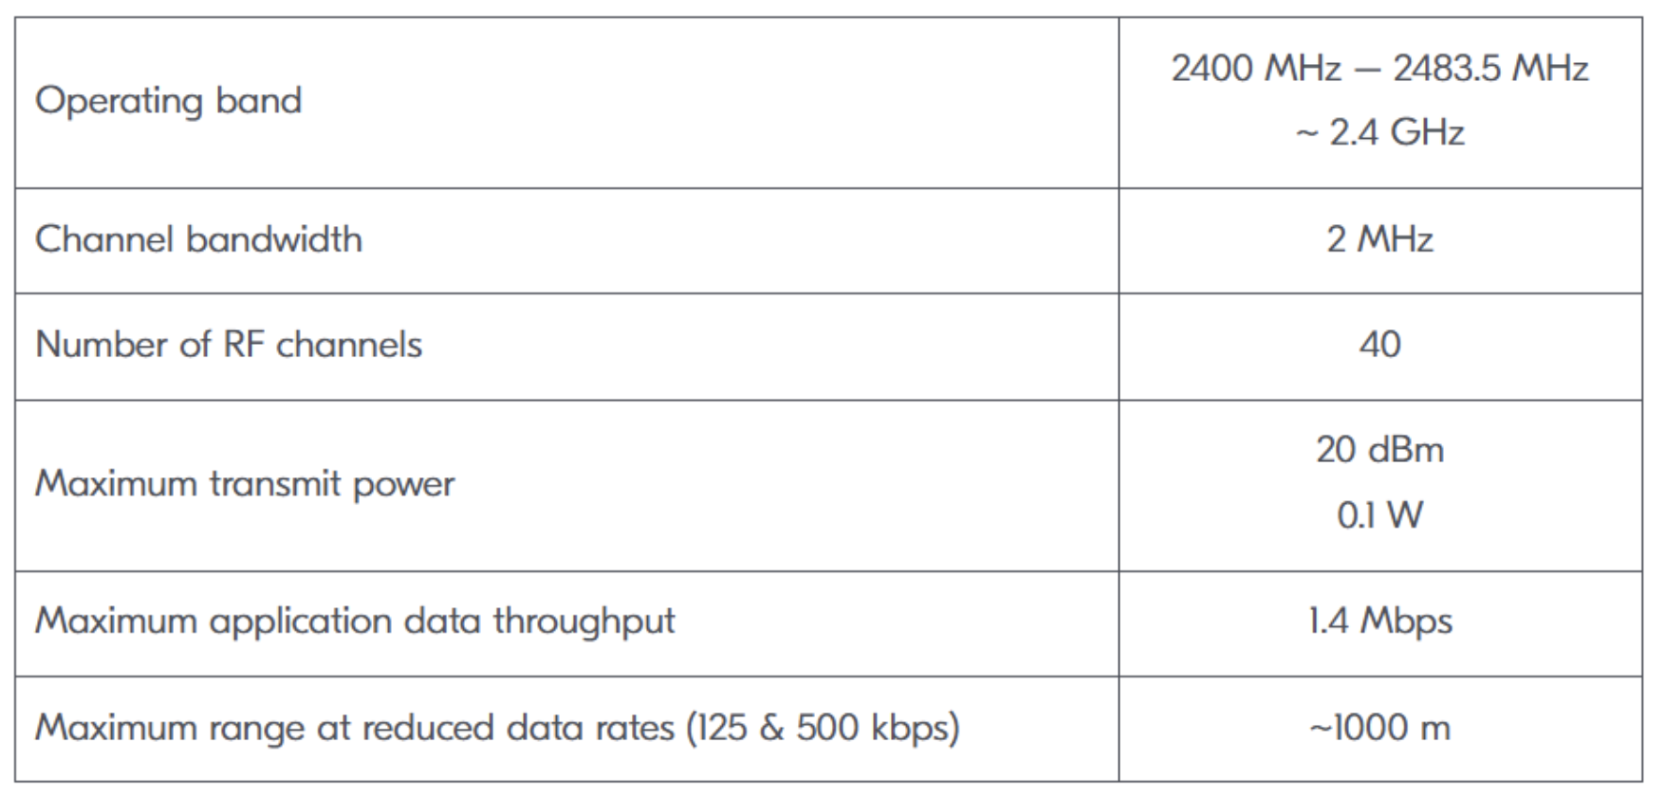
\includegraphics[width=\linewidth]{Bluetooth Low Energy/Screenshot 2024-08-15 at 23.25.43.png}
    \caption{BLE main characteristics. \cite{WhatBluetooth}}
    \label{ble_char}
\end{figure}

Some advantages of BLE include its lower cost compared to standard Bluetooth and the fact that most modern smartphones support it, making the development of applications easier and more cost-effective. To analyze the structure of BLE, the stack is explained, as shown in Figure~\ref{ble_stack}.



\begin{figure}[h]
    \centering
    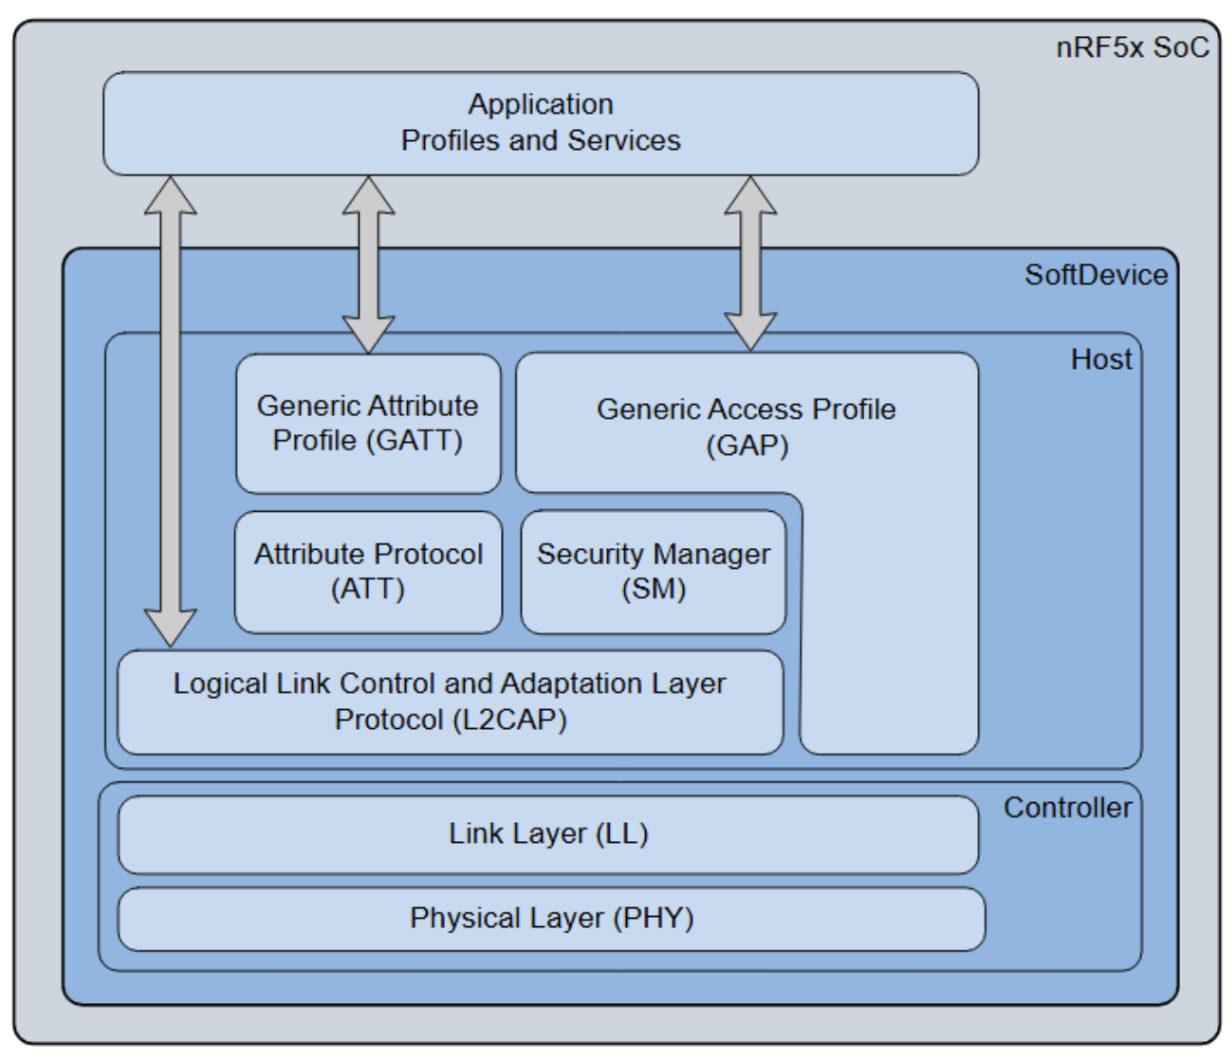
\includegraphics[width=\linewidth]{Bluetooth Low Energy/Screenshot 2024-08-15 at 23.25.52.png}
    \caption{BLE stack \cite{NordicSemiconductorInfocenter}}
    \label{ble_stack}
\end{figure}

The BLE stack is composed of two main sections: the controller and the host. The controller handles low-level tasks where timing is critical, while the host manages higher-level, more complex tasks. Specifically, the host establishes communication protocols and data exchange, while the controller generates radio waves and encodes data. These sections communicate via the Host Controller Interface (HCI). The uppermost layer is the application layer, which interfaces directly with the user and contains profiles, services, and characteristics.

\subsubsection{Physical Layer (PHY)}
The Physical Layer (PHY) is the lowest level of the BLE stack and defines the capabilities of Bluetooth radio waves, including modulation and coding schemes. It operates in the ISM band (2.402 GHz to 2.480 GHz), the same frequency band used by standard Bluetooth and Wi-Fi. The PHY is divided into 40 channels, each 2 MHz wide. Three of these channels are designated for advertising, while the remaining channels are used for communication. These channels frequently switch during a connection to avoid potential interference, and the advertising channels are evenly distributed across the ISM band to ensure continuous advertising without interruptions.

There are three PHY modes in BLE since version 5.0: 1 PHY, 2 PHY, and Coded PHY. 1 PHY provides a data rate of 1 Mbps and is supported by the oldest devices. 2 PHY doubles the maximum speed, reducing connection time and power consumption. Coded PHY extends the communication range by using error-correcting codes but sacrifices speed. In Coded PHY, each bit requires 2 or 8 characters, reducing the maximum throughput to 500 kbps or 125 kbps, respectively.

\subsubsection{Link Layer (LL)}
The Link Layer (LL) is responsible for data reception and processing, radio management, state control (advertising, scanning, connection maintenance), and time-critical tasks such as security functions (encryption and MIC computation). Since BLE version 5.0, the Link Layer supports seven different machine states: standby, advertising, scanning, initiating connection, connection, synchronization, and isochronous synchronization.

In standby mode, a device cannot send or receive data. In advertising mode, a peripheral device sends advertising packets and listens for connection requests. Scanning is the opposite, where a central device listens for advertising packets and then initiates a connection. In broadcast communication, the peripheral sends non-connectable or non-scannable advertising packets, and the central device only listens without establishing a connection.

\subsubsection{Host Controller Interface (HCI)}
The Host Controller Interface (HCI) manages communication between the host and controller sections. In microcontroller applications, both sections are integrated into a system on chip (SoC).

\subsubsection{Logical Link Control and Adaptation Layer Protocol (L2CAP)}
The Logical Link Control and Adaptation Layer Protocol (L2CAP) multiplexes data from multiple higher layers using channel identifiers. It also encapsulates data and ensures data integrity or triggers retransmissions if necessary.

\subsubsection{Security Manager (SM)}
The Security Manager (SM) is responsible for security-related functions such as encryption, pairing, and key exchange after a connection has been established.

\subsubsection{ATT and GATT}

Once data transmission on physical level has been explained, let's focus on how they are managed at logical level through ATT and GATT protocols.
The Attribute Protocol (ATT) defines the structure and exchange of BLE packets. It serves as an interface between peripheral and central devices, allowing them to share necessary characteristics. The Generic Attribute Profile (GATT) organizes this structure as shown in Figure~\ref{gatt_model}. 

\begin{figure}[h]
    \centering
    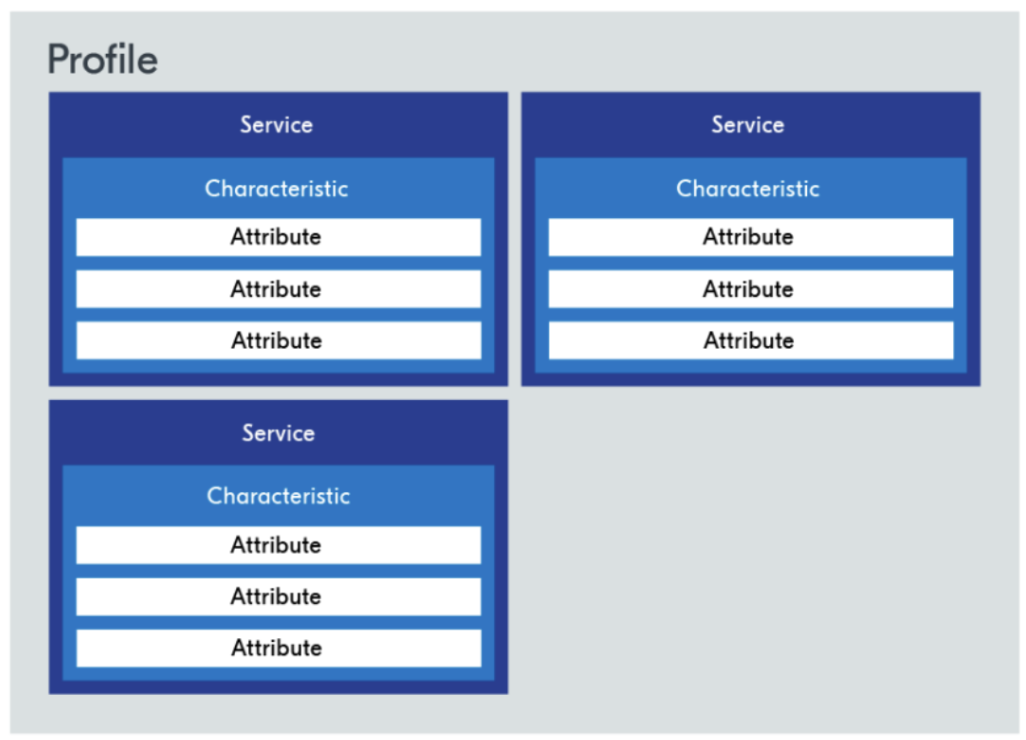
\includegraphics[width=\linewidth]{Bluetooth Low Energy/Screenshot 2024-08-15 at 23.26.01.png}
    \caption{GATT abstraction model \cite{ATTGATTData}}
    \label{gatt_model}
\end{figure}

A profile consists of services, which are collections of characteristics. Characteristics contain attributes. Six specific operations can be performed on characteristics:
\begin{itemize}
    \item \textbf{Write without response:} The client sends a command and does not require a response.
    \item \textbf{Write with response:} The client sends a command and expects a response.
    \item \textbf{Server response to client request:} The server responds to a client request.
    \item \textbf{Server notification:} The server notifies the client if a characteristic changes.
    \item \textbf{Indication:} Similar to a notification, but requires a client response.
    \item \textbf{Confirmation:} An acknowledgment packet sent by the client to the server.
\end{itemize}

\subsubsection{Generic Access Profile (GAP)}
The Generic Access Profile (GAP) defines the roles of each device and manages advertisement, security, and connection establishment. Roles depend on the specific application. For connection-oriented communication, the roles are central (scanning and initiating the connection) and peripheral (advertising and accepting the connection). For broadcast communication, the roles are broadcaster (sending advertising packets) and observer (listening to packets). Some devices may operate in multiple roles simultaneously, known as multi-role, for example, receiving data from a sensor while also sending data.


\section{Security in Bluetooth Low Energy}

Bluetooth Low Energy, as well as all wireless technologies, is potentially exposed to possible attacks, such as sniffing or jamming. When discussing wireless communications, a hacker does not necessarily need to manage the physical device to control it. These attacks could potentially damage the safety of data transfer or the privacy of the patient since the intended device has a medical purpose and the data transferred could be sensitive. Moreover, medical devices require a minimum level of security to obtain pre-market approval.

The paper published in the Elsevier journal \cite{caesar2022survey} provides a brief explanation of the security features related to the specific intended Bluetooth Low Energy version. These can be summarized in the Table below.

\begin{figure}[H]
    \centering
    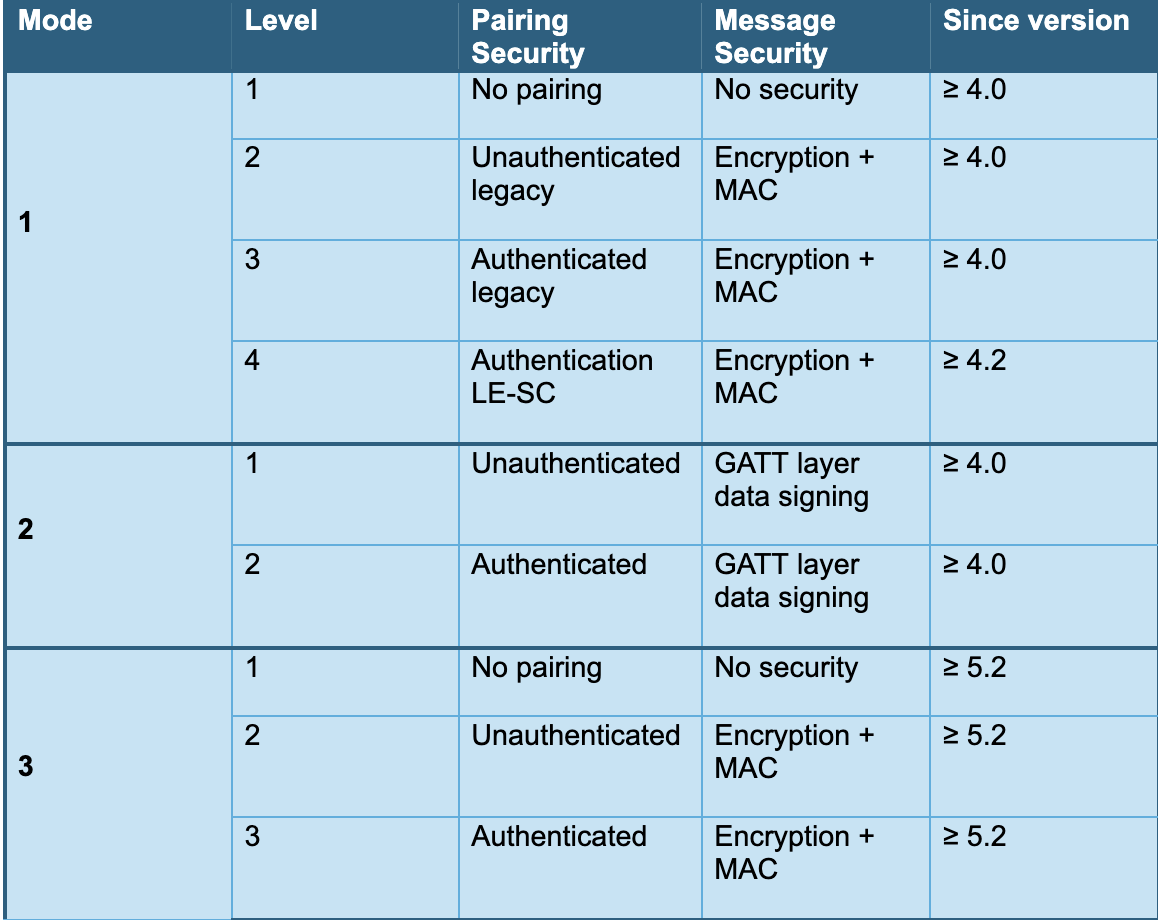
\includegraphics[scale=0.7]{Bluetooth_Security/1.png}
    \caption{Bluetooth security table \cite{casarSurveyBluetoothLow2022}}
    \label{bluetooth_sec_1}
\end{figure}

As seen in Table \ref{bluetooth_sec_1}, security in BLE is organized into modes and levels to distinguish between different security features. Developers can choose to implement a specific mode based on the purpose of the intended application and the features needed. In particular, mode 1 refers to the decision of device pairing, mode 2 is based on the verification of the authenticity of the data exchanged, and mode 3 is intended for broadcast applications which might need encryption or other features to protect data transfer.

\subsection{Pairing}

The pairing procedure involves the agreement of keys between the devices involved in the connection, to enable the encryption of exchanged data. This procedure is required for all security modes and levels, as shown in Table~\ref{bluetooth_sec_2}, except for Mode 1 Level 1 and Mode 3 Level 1, which provide no security features at all. The pairing procedure is shown in detail below.

\begin{figure}[H]
    \centering
    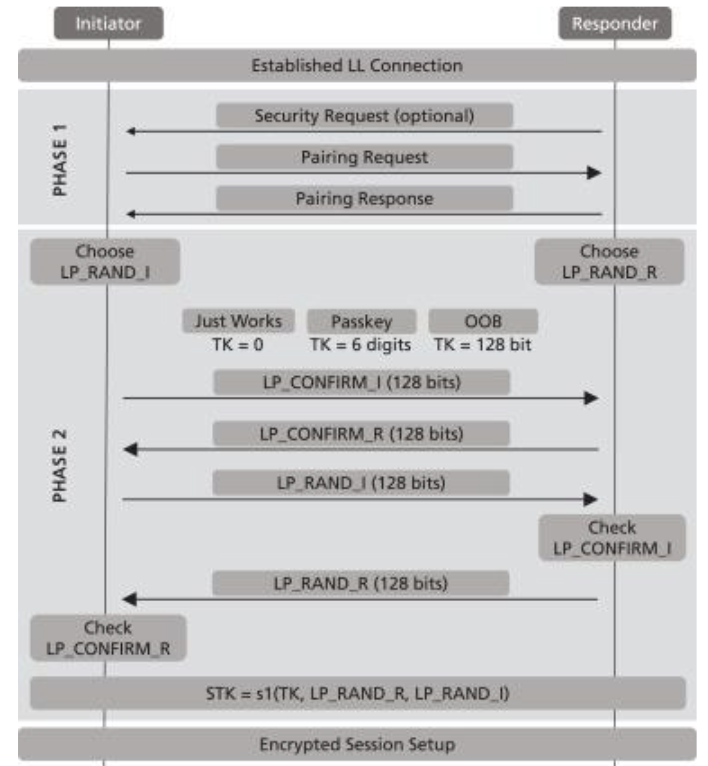
\includegraphics[scale=0.7]{Bluetooth_Security/2.png}
    \caption{Bluetooth pairing table \cite{casarSurveyBluetoothLow2022}}
    \label{bluetooth_sec_2}
\end{figure}

As shown in the figure, the pairing procedure consists of two different phases. The first phase is responsible for exchanging features related to security, such as the association modes, whether or not Man-In-The-Middle (MITM) protection is required, and the input/output capabilities of both devices to agree on the security level and mode to establish. Additionally, during this phase, the devices exchange possible bonding requests, which will be explained in detail later in this section. Once phase 1 is complete, phase 2 occurs, where the actual exchange of keys happens. These keys will be used to encrypt the connection in the future.

Based on the information exchanged in phase 1, the mode of pairing is chosen. As shown in Figure 4.12, these modes could be different. Specifically, the lowest security value is provided by the “Just Works” method, where no authentication method is required. This can be used in applications where at least one of the devices has neither input nor output capabilities. When possible, this method should be avoided in favor of one that guarantees a higher level of security. When the “Just Works” method is chosen, the Temporary Key (TK) is set to 0, and the user is simply asked to accept the connection, as reported in \cite{nordic_academy}. When the Passkey method is selected, it indicates that all devices involved in the connection have at least one input/output capability, and the connection is authenticated. The specific authentication method varies based on the intended application. For example, if one device has only input capabilities and the other only output, the user may be required to enter the password displayed on the first device into the second device. Another example is when both devices have only input capabilities; in this case, the user may need to enter the same password on both devices. These methods of authentication are called “Passkey Entry” and require at least one of the devices to have keyboard capabilities. Another method is “Numeric Comparison,” which requires only output capabilities. Both devices display a password, and the user must confirm that these are equal on both devices. For both methods, the password is 6 digits long. The last method, “Out of Band,” requires another communication method like NFC to exchange the password, which is 128 digits long in this case. To summarize, Figure 3.13 shows a recap of the pairing authentication methods based on the input/output capabilities of the devices involved. The password exchanged in phase 1 is known as TK (Temporary Key).

\begin{figure}[H]
    \centering
    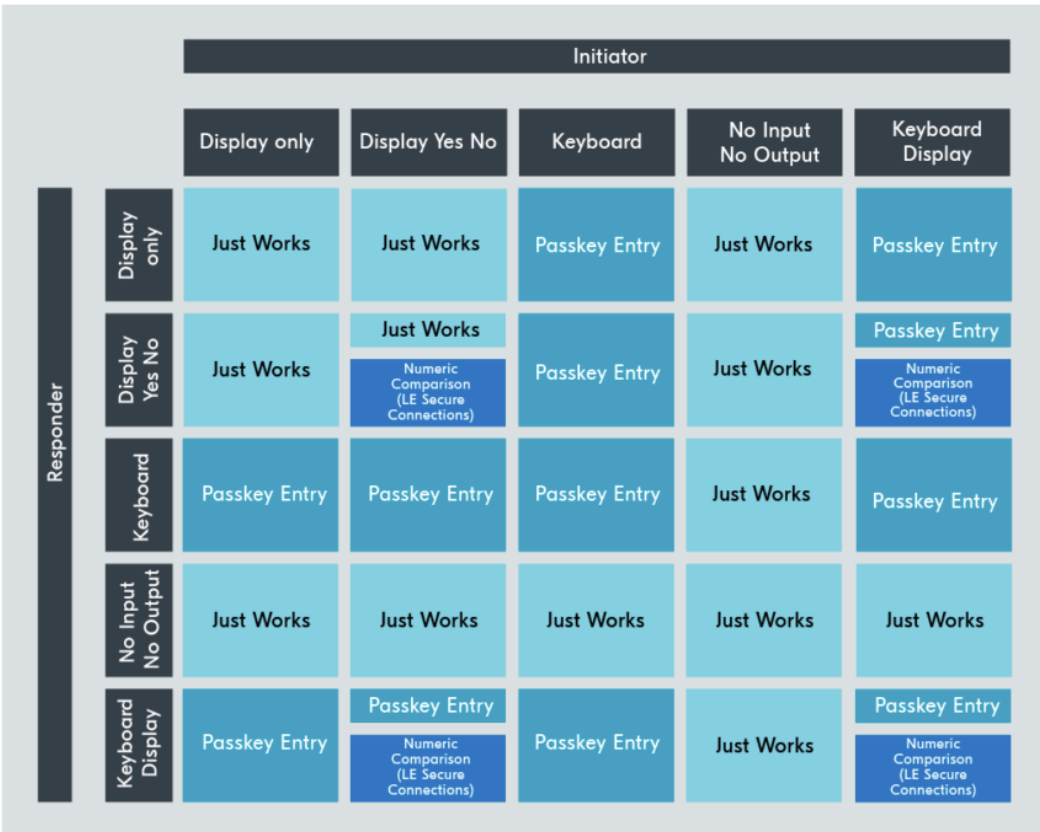
\includegraphics[scale=0.7]{Bluetooth_Security/3.png}
    \caption{Bluetooth pairing table \cite{PairingProcess}}
    \label{bluetooth_sec_3}
\end{figure}

The actual authentication, however, is done at a lower level. As shown in Figure~\ref{pairing_procedure}, both devices generate a random value: \texttt{LP\_RAND\_R} for the peripheral and \texttt{LP\_RAND\_I} for the central device. These values, together with the information exchanged in phase 1 and the TK, generate the confirmation values \texttt{LP\_CONFIRM\_I} and \texttt{LP\_CONFIRM\_R}. Once the exchange of these two confirmation values is performed, their reliability is checked by exchanging the previously generated random values \texttt{LP\_RAND\_I} and \texttt{LP\_RAND\_R}. If the check is successful, the two random values, along with the TK, are used to generate the Short-Term Key (STK). The pairing procedure then ends, and the last computed value STK will be used in future procedures to encrypt the connection.

\section{Communication system}

\subsection{Previous code implementation}

As show in the introduction, Senseback is an implanted device which communicates with an external unit through Bluetooth Low Energy. The starting point for the firmware code of this communication was previously developed by Chiara Quartana during her Master Thesis for PNRelay. Our master thesis purposes improvement and additional features on the previous code, which presents some limitations.

\begin{figure}[H]
	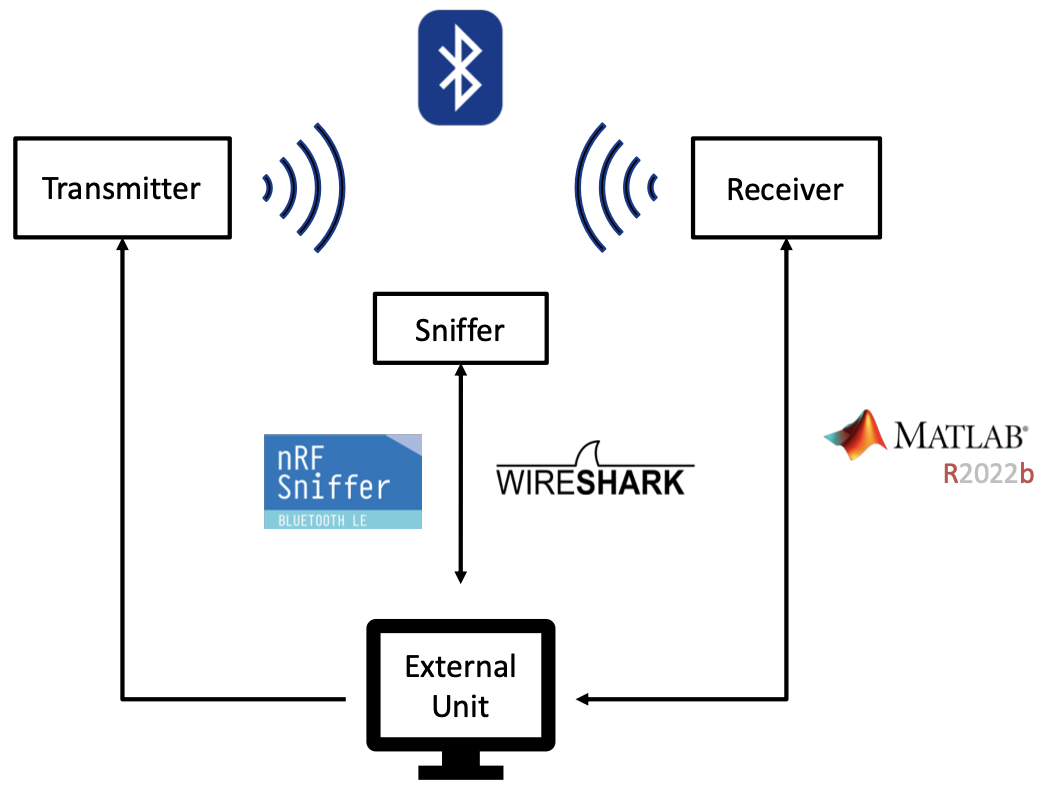
\includegraphics[scale=0.3]{prev1.png}
	\centering
    \label{prev_1}
    \caption{Previous model implementation}
\end{figure}

Figure 1: BLE communication between Senseback and external device
The general architecture for the previous code is shown in Figure 2.

\begin{figure}[H]
	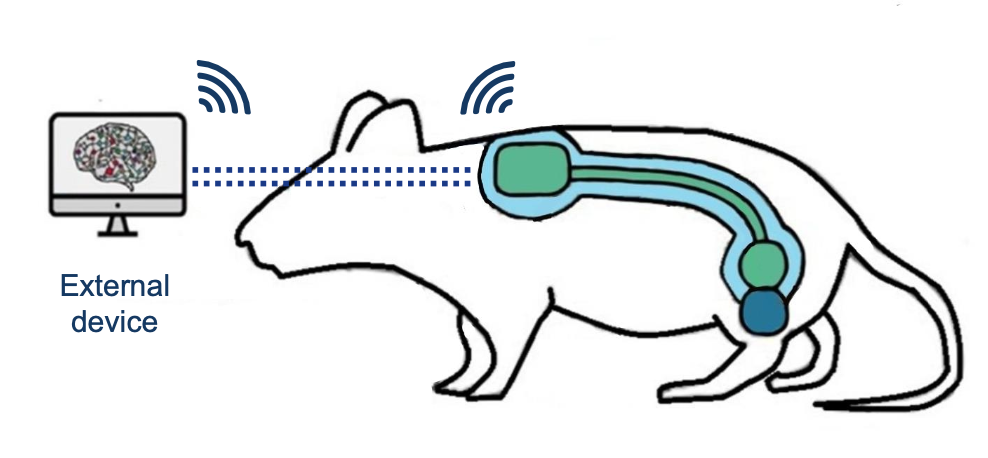
\includegraphics[scale=0.3]{prev2.png}
	\centering
    \label{prev_2}
    \caption{Previous implementation}
\end{figure}



Figure 2: Previous implementation, setup of the experiment.
As is it possible to see, two main devices facilitate communication: the transmitter and the receiver. For the experiment, two identical nRF52 Development Kits (DKs) \cite{NRF52DKDevelopment} were used as the transmitter and receiver. These boards were thought to be employed just for testing, the final implementation, in fact, will replace the transmitter board with the Senseback device, and the external unit will serve as the receiver. Both boards were powered and controlled through the external unit, which was a PC connected via serial ports.
External unit allowed the user to manage the communication by sending "START," "STOP," and "RESET" commands. This was done thanks to the usage of a Matlab script. These commands were transmitted through the serial port and received by the receiver using Universal Asynchronous Receiver/Transmitter (UART). UART is a common serial communication protocol used for connecting microcontrollers and other devices, often facilitated by USB-UART converters \cite{LessonSerialCommunication}.
For both the transmitter and receiver, separate codes were implemented to manage communication. The first code set, designated as "Offline," was designed to test communication with a fixed number of packets. Specifically, 32,400 packets of one byte each were transmitted. The test began when the user entered the "START{\textbackslash}n" command through MATLAB, giving the signal to the transmitter to start sending packets. This test ended when all packets were sent. The "Online" communication, on the other hand, simulated real-time behaviour with no predefined packet count. This test also begun once the user digited the "START{\textbackslash}n" command, but it required also a "STOP{\textbackslash}n" command to end. Lastly, the "RESET{\textbackslash}n" command was just used in those cases in which it was necessary to restart the communication from the beginning.
Upon receiving the appropriate command in MATLAB, the external unit would send it to the receiver via UART, which then relayed the command to the transmitter through BLE. The transmitter would start sending data to the receiver upon receiving the "START{\textbackslash}n" command and stop when it received the "STOP{\textbackslash}n" command or all packets had been sent, depending on the test mode. After receiving the packets, the receiver printed the data to the serial port, allowing the external unit to read it through MATLAB. 
Last element of the previous setup is the sniffer. The purpose of this was to detect the packets exchanged from transmitter and receiver, including possible retransmissions during the communication. The chosen software to play this role is Wireshark (v.4.0.6) with the nRF Sniffer Tool (v.4.1.1), provided by Nordic Semiconductor©.
All the codes used for this setup are deeply analysed below.

\subsection{Matlab scripts}

To achieve the two main objectives of communication control and data verification through a serial port, two separate MATLAB scripts were created. The first script is designed for offline testing, the second one for online. Here's how they work:
Both scripts start by creating a vector that simulates the incoming ADC samples from a Senseback device. These samples are in uint16 format. Each value is then split into two uint8 values using the MATLAB function typecast, ensuring that the data is converted without losing information. The next step is to set up the serial port with a baud rate of 115200 bps, whose limit is imposed by the UART communication. After setting the baud rate, the serial port is flushed to ensure it's clear before communication begins.
The scripts, instead, differ in the following ways:
Commands: In the offline test script, only one command is required from the user, while the online test script requires two commands, the start and the stop of the communication.
Data Reception: The online script does not include any data reception functionality due to memory limitations and the slower baud rate. In contrast, the offline script does receive data from the serial port.
The online test script is simpler, focusing on generating the data and ensuring the serial port is set up properly. There is no data reception because of the limitations mentioned earlier.
The offline test script uses a callback function to handle data reception. It uses the MATLAB configureCallback function to call the readData function each time new data is received from the selected serial port. The purpose of this function is to store the incoming data in a vector and keep track of the total data received. The callback function is turned off when the last two values are both 255 (indicating the end of a data sequence). Once all data is received, it can be converted back to uint16 using typecast and organized into a matrix for plotting and further analysis. The offline test script can then compare the received data with the data originally generated in MATLAB to ensure its accuracy and reliability.

\begin{figure}[H]
	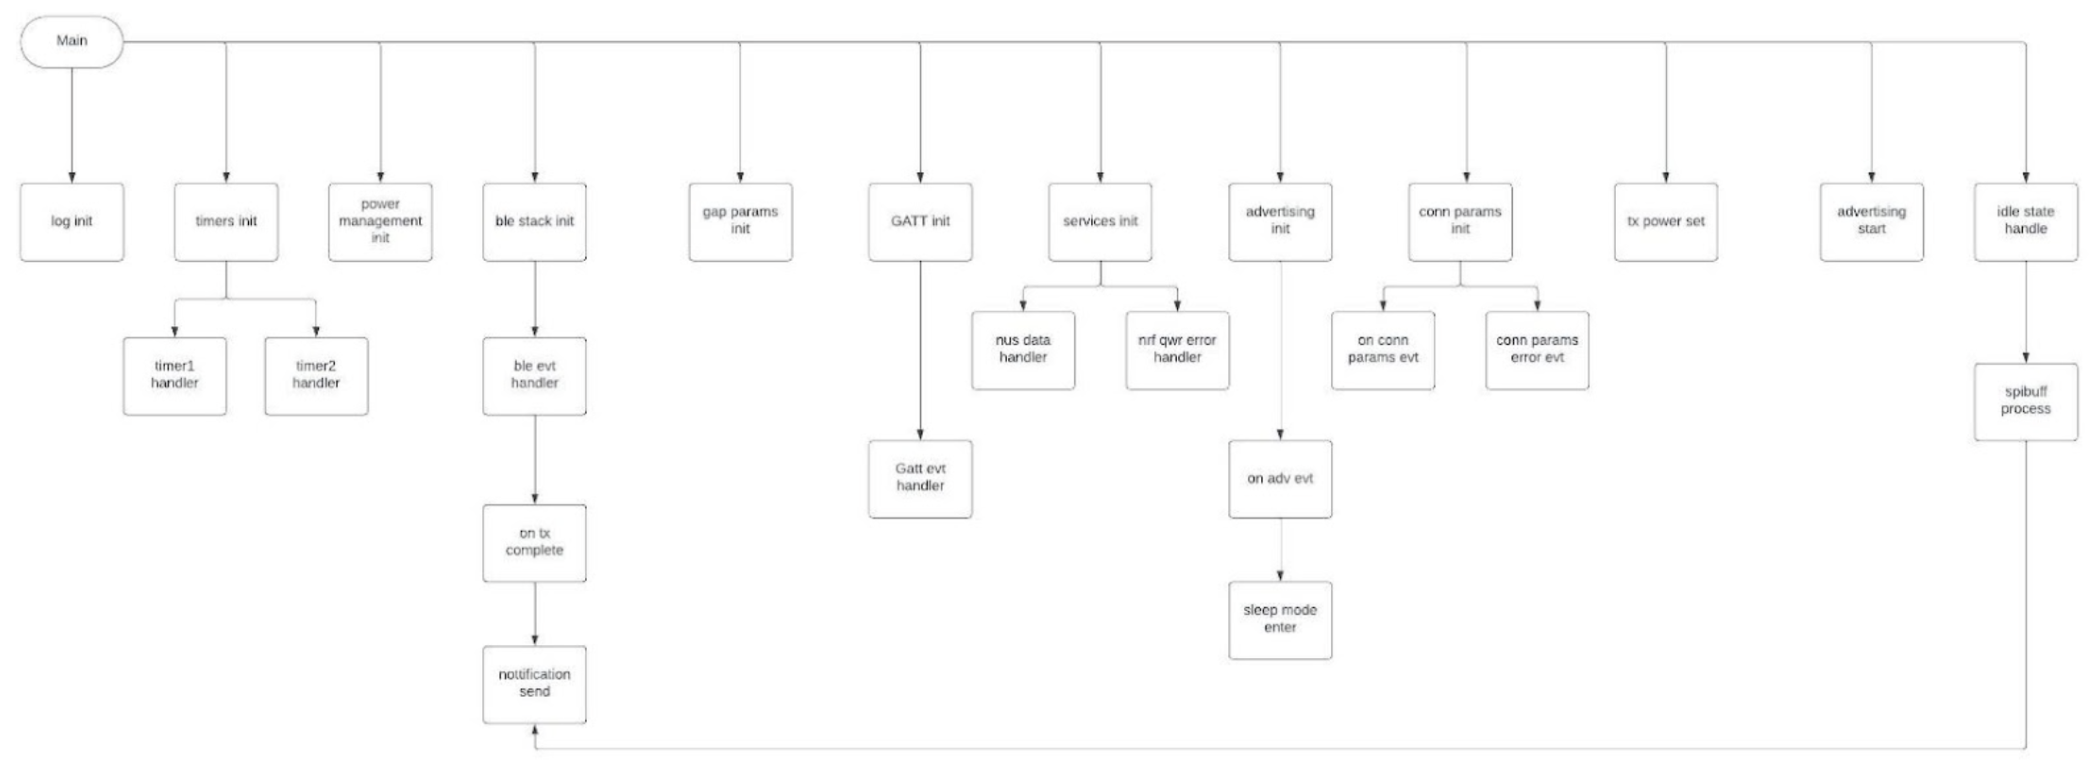
\includegraphics[scale=0.3]{Previous Implementation/Screenshot 2024-08-15 at 10.59.58.png}
	\centering
    \label{prev_3}
    \caption{Offline transmitter code}
\end{figure}


\subsection{Offline transmitter code}
Figure 3 illustrates a flow chart of the offline code for the transmitter. Each block represents a distinct function. Below is a brief explanation of each one.


\textbf{Log init}: \quad This function initializes the log module. This module provides logging capabilities for the intended embedded application \cite{NordicSemiconductorInfocentera}. It has different usages such as debugging, which means to provide diagnosis for possible issues, info, which implies to check whether or not the application works as expected, warning, so indications about something unexpected which is happened, and error in those cases in which the software is not able to execute one of the functions.

\textbf{Timers init}: \quad This function initializes the timers. For the offline code of the transmitter, two timers have been used. The first one is the timer responsible for data generation, and the second one is responsible for monitoring the total time required for data generation, data pre-processing, and sending to the central device. The two timers are both equally initialized, with the frequency set to 2 MHz for both.

The main difference between these two timers is given by the functions \texttt{nrfx\_timer\_us\_to\_ticks} and \texttt{nrfx\_timer\_ms\_to\_ticks} for the first and the second timer, respectively. These functions create an interrupt each time the timer reaches the specified value, which is 12.5 $\mu$s for the first one and 1 ms for the second. The value of 12.5 $\mu$s has been chosen to simulate the arrival of samples coming from the ADC in the actual application; in fact, 12.5 $\mu$s represents a frequency of data generation of 80 kHz.

\textbf{Timer 1 handler}: \quad This function is responsible for data generation. Firstly, it checks whether the transmission is active, i.e., whether the command \texttt{START} has been received from the central device. If it is active, a new data \texttt{CNT} is generated. Data generation is done as a step, so each new value is equal to the previous one plus one. \texttt{CNT} is a \texttt{uint16\_t} variable. This choice is made because the ADC samples have 10 bits size, and the \texttt{uint16\_t} variables are the smallest ones which guarantee that the samples are saved without wasting information, which would occur if a \texttt{uint8\_t} variable were chosen.

Once the new \texttt{uint16\_t} data is generated, it is put into the ring buffer \texttt{uartRx}. \texttt{Ringbuf} is a data structure that uses a single, fixed-size buffer as if it were connected end-to-end. This structure is useful for buffering data streams, where data needs to be overwritten as new data comes in, particularly when the buffer is full. It's commonly used in scenarios where the producer and consumer operate at different rates, as in this case. The size of \texttt{uartRx} has been set to 16384 \texttt{uint16\_t} variables, representing the maximum size imposed by the RAM storage limits.

Once \texttt{CNT} has been put into the ring buffer, the function \texttt{data\_arrived}, which is responsible for counting the number of data generated, is incremented by one. Then, it is checked whether the new value generated is the first one using the boolean variable \texttt{first}. If this is still true, as initialized, it means that the new data generated is the first one, so \texttt{timer2} starts counting from a time elapsed equal to zero milliseconds. When the condition \texttt{first=true} is triggered, the boolean variable \texttt{first} is set to \texttt{false}, thus avoiding entering the previous condition in the next cycle and starting \texttt{timer2} again.

The last step for this function is to check whether the data generation process has arrived at the end. This is done by checking the value that the variable \texttt{data\_arrived} has reached. If this value is greater than the value imposed by \(\left(\frac{\texttt{DATA\_TO\_SEND} - 2}{2}\right) - 1\), the condition is triggered. For the offline test, the \texttt{DATA\_TO\_SEND} variable is equal to 32400 and represents the number of bytes that should be sent to the central device to complete an offline test. Consequently, the condition is triggered when the variable \texttt{data\_arrived} has reached a value of 16198, which also represents the number of samples arrived from the ADC. The choice for this condition triggering will be explained in detail when discussing the \texttt{spibuff} process function, which is responsible for data preprocessing before sending.

Once the condition is triggered, the \texttt{data\_arrived}, \texttt{first}, and \texttt{CNT} values are reset, and the last 16-bit value is put into the ring buffer: 65535. This value represents the highest value in binary that can be represented using 16 bits. It is, in fact, a sequence of 16 bits all set to 1. Then, the boolean variable \texttt{transmission} is set to \texttt{false}, indicating that data generation is finished.

\textbf{Timer 2 handler}: \quad is the timer responsible for the computation of the total time elapsed during the data generation, data preprocessing, and data sending processes. This function increments the variable \texttt{total\_time\_elapsed\_ms} by one each time the interrupt is triggered, so each millisecond. In this way, \texttt{total\_time\_elapsed\_ms} provides a timestamp of the current total time elapsed in milliseconds.


\textbf{Power management init}: \quad this function initializes the power management module, which handles power management features. \cite{NordicSemiconductorInfocenterb}

\textbf{Ble stack init}: \quad this function is responsible for the initialization of the SoftDevice and BLE event interrupts. A SoftDevice is a precompiled and linked binary software implementing a wireless protocol developed by Nordic Semiconductor. \cite{NordicSemiconductorInfocenterc} In this function, it is first requested to enable the SoftDevice using the \texttt{Nrf\_sdh\_enable\_request} function. Once the SoftDevice has been enabled, it is configured through the function \texttt{Nrf\_sdh\_ble\_default\_cfg\_set} by using the default settings specified in the SoftDevice handler BLE configuration. Finally, the functions \texttt{Nrf\_sdh\_ble\_enable} and \texttt{Nrf\_sdh\_ble\_observer} respectively enable the BLE stack and register a handler for BLE events.

\textbf{Ble evt handler}: This function manages the different BLE events. It first creates a pointer to the specific GAP events, then a switch gives the instructions for each different event.

\begin{itemize}
    \item \textbf{First case:} the device is connected. If this case is triggered, a log and the usage of LEDs, enabled through the function \texttt{bsp\_indication\_set}, indicate to the user that the connection has been correctly performed. The connection handle is then stored in the variable \texttt{m\_conn\_handle}. The connection handle is a value provided by the BLE stack that uniquely identifies a connection with another BLE device \cite{BluetoothLowEnergy2016}. Then, the function \texttt{nrf\_ble\_qwr\_conn\_handle\_assign} assigns a connection handle to the given instance of the Queued Writes module \cite{NordicSemiconductorInfocenterd}. Ultimately, the data rate (PHY) is set to 2 Mbps for both the TX and RX BLE characteristics.
    
    \item \textbf{Second case:} the device is disconnected. In this case, it is logged to the user that a disconnection occurred, and the connection handle is set to invalid.
    
    \item \textbf{Third case:} PHY update request. In this case, the data rate is automatically changed to respond to a PHY update request.
    
    \item \textbf{Fourth case:} security parameters request. In this implementation, security features are not implemented, which means that the reply to the security parameters request is that pairing is not supported.
    
    \item \textbf{Fifth case:} system attribute access pending, such as bonding information \cite{NordicSemiconductorInfocenterf}. Again, in this case, no system attribute is stored.
    
    \item \textbf{Next cases:} timeout events. If these are triggered, the connection is terminated.
    
    \item \textbf{Last case:} transmission has been completed. If this happens, the function \texttt{on\_tx\_complete} is called.
\end{itemize}


\textbf{On Tx complete}: This function manages the packet transmission queue mechanism. If the \texttt{BleTxBusy} variable is true, indicating that a packet has not been sent due to the transmission channel being busy, the variable is reset to false. Then, the \texttt{notification\_send} function is called to attempt retransmission. This ensures that no packets are lost, as transmission attempts continue until successful completion.

\textbf{Notification send}:
This function oversees the data transmission process and calculates the transmitter's throughput. Initially, a \texttt{uint32\_t} variable \texttt{err\_code} is set to \texttt{NRF\_SUCCESS}, indicating no errors. Before sending data to the receiver, the function checks two conditions:

\begin{itemize}
    \item \textbf{Error Check}: It verifies that \texttt{err\_code} remains \texttt{NRF\_SUCCESS}, ensuring no transmission errors have occurred.
    \item \textbf{Data Availability Check}: It ensures that the \texttt{uint16\_t} variable \texttt{txRdPtr} (index tracking the last number of bytes sent) is less than \texttt{txSize} (total number of available data bytes). This ensures sufficient new data is pre-processed and ready for transmission.
\end{itemize}

If both conditions are satisfied, the length of the new packet to be sent, stored in the \texttt{length} variable, is updated to \texttt{txSize - txRdPtr}. This data of this length is then sent via the \texttt{ble\_nus\_data\_send} function and \texttt{err\_code} is updated accordingly. If \texttt{ble\_nus\_data\_send} completes successfully without errors, \texttt{txRdPtr} is incremented by the size of \texttt{length}, and the \texttt{data\_sent} variable, which tracks the total bytes sent to the central device, is also increased by \texttt{length}. 

Next, the function checks if the transmission has reached the end by verifying if the last two bytes sent are both 255. Since 255 is the maximum value representable with 8 bits, this check ensures the last \texttt{uint16\_t} variable in the ring buffer \texttt{uartRx} (set to 65535 in \texttt{timer1\_handler} function) has been sent. If true, the total elapsed time is calculated by converting the timer ticks of \texttt{timer2} to milliseconds. The throughput is then calculated.
\[
\text{throughput} = \frac{\text{data\_sent} \times 8}{\text{total\_elapsed\_time}}
\]
All relevant values, including the number of waits, are logged. If \texttt{ble\_nus\_data\_send} function returns an error, indicating an unsuccessful transmission, \texttt{bleTxBusy} is set to true, and the wait counter is incremented. Finally, if \texttt{txRdPtr} is greater than or equal to \texttt{txSize}, the \texttt{txActive} variable is set to false, indicating that another packet can be pre-processed.

\textbf{Gap params init}: this function sets the necessary Generic Access Profile (GAP) parameters of the device, such as security level and the name of the device. In this implementation, since security features have not been implemented, function \texttt{BLE\_GAP\_CONN\_SEC\_MODE\_SET\_OPEN} sets the level of security at the minimum, meaning that the board is totally open. The other parameters that are set in this function are the ones related to the packet exchanges such as minimum and maximum connection interval (CI), the slave latency and the connection superior timeout. These parameters have a great impact on the overall throughput that would be reached in the end.

\textbf{Gatt init}: This function initializes the Generic Attribute Profile (GATT) library. It also sets the Attribute Protocol (ATT) Maximum Transmission Unit (MTU). This parameter defines the maximum amount of data that can be exchanged by a single BLE packet, specifically for the peripheral side. For this application, the MTU has been set to \texttt{NRF\_SDH\_BLE\_GATT\_MAX\_MTU\_SIZE}, which corresponds to a value of 247 bytes, the maximum achievable with BLE version 5.2. A high value for \texttt{GATT\_MTU} generally implies higher efficiency for data exchange and consequently, a higher throughput. In fact, with a single exchange, it is possible to send a larger amount of data, minimizing the wasted time due to latency.

\textbf{GATT Event Handler}: this function handles events coming from the GATT library. It first checks whether the event triggering is caused by the current connection by looking at the connection handle stored in the variable \texttt{m\_conn\_handle}. In this implementation, the condition will always be triggered since there is only one connection, which is point-to-point. It also checks, together with the previous condition, whether the event that occurred is an update of the GATT ATT MTU. If both these conditions are satisfied, then the \texttt{m\_ble\_nus\_max\_data\_len} variable is updated to the effective ATT Payload for the connection, which is equal to ATT Data minus the two headers shown in Figure 4, specifically, the Op Code and the Attribute Handle.

\begin{figure}[H]
	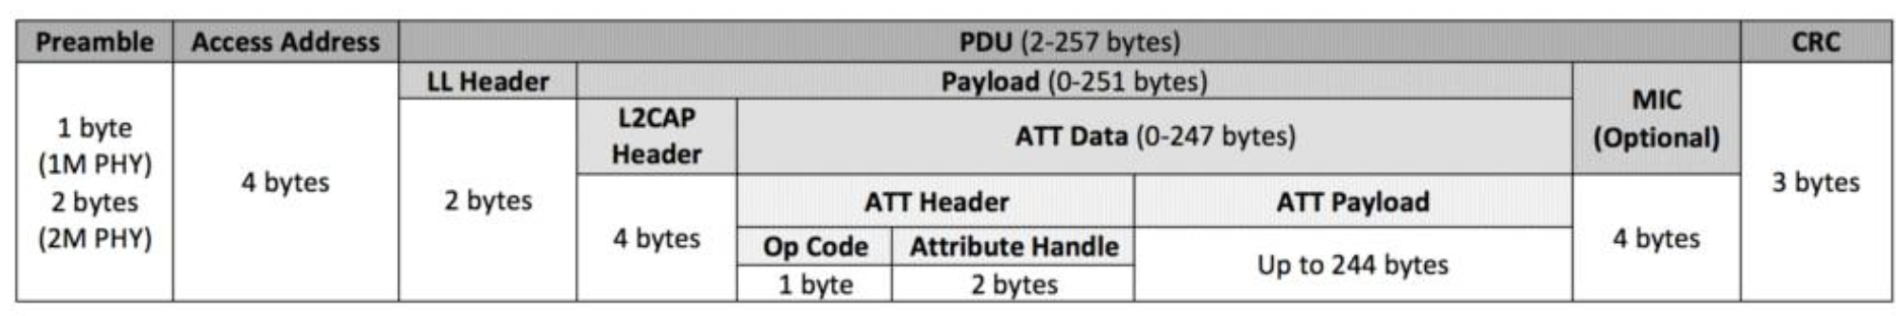
\includegraphics[scale=0.3]{Previous Implementation/Screenshot 2024-08-15 at 11.00.56.png}
	\centering
    \label{prev_4}
    \caption{Package structure \cite{afanehBluetoothSpeedHow2023}}
\end{figure}

Once this value is updated, the desired values for ATT MTU of the central and peripheral devices are logged to allow the user to check whether they are the same, ensuring that both devices agree on the maximum achievable value.

\textbf{Services Init}: this function is used to initialize all the services which will be used in the application. For the intended purposes, the services that are initialized are two: Queued Write Module (qwr) and NUS module. The qwr module handles prepare write, execute write, and cancel write commands. It also manages memory requests related to these operations. The NUS module is a custom Bluetooth Low Energy (BLE) service designed to emulate a UART (Universal Asynchronous Receiver/Transmitter) over BLE. This allows devices to communicate wirelessly in a manner similar to serial communication over a wired connection.

\textbf{NUS Data Handler}: this function manages the start, stop, and reset occurrences of the BLE communication by checking the command received from the central device. The function starts with an \texttt{if} condition, which checks whether a command is received by the peripheral device via NUS. If this is the case, the value of the received string is saved into the variable \texttt{dongle\_command}. Then, the actual value of the string is checked. If the received string through \texttt{ble\_nus} is equal to START, this means that the user has sent the command to begin communication. Consequently, the boolean variable \texttt{transmission} is set to \texttt{true}, indicating that transmission should start, \texttt{timer1} is enabled, and \texttt{timer2} is reset. In this way, data generation starts, and it is ensured that the total time elapsed counter starts from 0. If instead, the command received is equal to RESET, then the \texttt{CNT} variable is set to 0, meaning that data generation is reset to the beginning. Finally, if the received command is equal to STOP, then \texttt{timer1} is disabled. By stopping the data generation, no more data will be available for transmission, and the whole process of data sending will stop.


\textbf{NRF QWR Error Handler}: this function handles Queued Write Module (qwr) errors. A pointer to this function will be passed to each service which may need to inform the application about an error.

\textbf{Advertising init}: This function is used to initialize the advertising functionality of the peripheral device. When a BLE device broadcasts its presence, it sends out advertising packets that can include various types of information, such as device name, service UUIDs, manufacturer-specific data, and appearance. For the current application, the advertising packets include the device’s full name but not the appearance data. Appearance data is a predefined value that indicates the type or category of the device. This value is used to give a general idea of the device's functionality without requiring a full connection. It helps other BLE devices and applications quickly identify what kind of device they are encountering. The choice of not including the appearance value in the advertising packets could be made both for privacy reasons and for saving space for other information. Another included parameter in the advertising packets is the advertising flag field, which in this case is set to \texttt{BLE\_GAP\_ADV\_FLAGS\_LE\_ONLY\_LIMITED\_DISC\_MODE}, meaning that the device only supports BLE and not classic Bluetooth, and that the device will be in a discoverable state for a limited time. 

Furthermore, UUIDs should be defined. A UUID is a unique identifier for services offered by the BLE device. The function \texttt{advertising\_init} first computes the number of UUIDs that are present in the \texttt{m\_adv\_uuids} array, then it sets \texttt{uuid\_cnt} to that value. Then, \texttt{init.srdata.uuids\_complete.p\_uuids} sets the pointer to the array of UUIDs, which tells the program where to find the list of UUIDs that describe the services the BLE device offers. Finally, the advertising settings are set. In particular, fast advertising mode is enabled, meaning that the device will advertise itself frequently, making it quicker to be discovered. 

The last two parameters for advertising are set as follows:
\begin{itemize}
    \item \texttt{APP\_ADV\_INTERVAL}, which defines how often the device will send out advertising packets when in fast advertising mode. In this case, the \texttt{APP\_ADV\_INTERVAL} parameter is set to 64 in units of 0.625 ms, which corresponds to 40 ms.
    \item \texttt{APP\_ADV\_DURATION}, which defines how long the device will stay in fast advertising mode before stopping or switching to another mode. In this case, this value is equal to 18000 in units of 10 ms, which corresponds to 180 s.
\end{itemize}

Ultimately, the event handler function for advertising events is set, which will handle various events related to advertising, such as starting, stopping, or timing out. Once this configuration has been completed, the advertising module is initialized using the function \texttt{ble\_advertising\_init}, and \texttt{ble\_advertising\_conn\_cfg\_tag\_set} sets the connection configuration settings tag for the advertising instance.


\textbf{On adv evt}: this function is responsible for handling the advertising events. Two possible cases are considered:
\begin{itemize}
    \item \textbf{Fast Advertising Event:} If this event occurs, LED1 starts blinking to signal that the device is in the advertising phase.
    \item \textbf{Advertising Idle Event:} If this event occurs, the \texttt{sleep\_mode\_enter} function is called.
\end{itemize}

\textbf{Sleep Mode Enter}: this function puts the chip into sleep mode to save battery when the device is not in use. To signal the state of the board, the behavior of the LEDs is changed. Specifically, for the idle case, all LEDs are turned off. The \texttt{bsp\_btn\_ble\_sleep\_mode\_prepare} function is used to prepare the wakeup buttons before going into sleep mode \cite{nordic_semi}. Lastly, the system is put into sleep mode using the \texttt{sd\_power\_system\_off} function.


\textbf{Connection Parameters Initialization}: this function initializes the connection parameters module that will be used when establishing and maintaining a connection with a central device. The pointer to the initial connection parameters is set to NULL, meaning no initial parameters are provided. The delay before the first update of the connection parameters and the following parameters update delay are set to 5000 ms and 30000 ms respectively. These parameters describe the delay before the first update of the connection parameters is attempted and the delay between subsequent attempts if the first attempt fails. The maximum number of attempts to update the connection parameters before giving up the connection parameter negotiation is set to three. If the connection parameter update procedure fails, disconnection does not happen since \texttt{cp\_init.disconnect\_on\_fail} is set to false. The \texttt{cp\_init.start\_on\_notify\_cccd\_handle} sets the handle of the Client Characteristic Configuration Descriptor (CCCD), which triggers the connection parameter update procedure. \texttt{BLE\_GATT\_HANDLE\_INVALID} indicates that the connection parameter update procedure is not started by any specific CCCD. The functions \texttt{on\_conn\_params\_evt} and \texttt{conn\_params\_error\_handle} are assigned to manage possible changes or updates to connection parameters and handle errors during the connection parameters update process. All the settings chosen inside the \texttt{conn\_params\_init} function become effective through the \texttt{ble\_conn\_params\_init} function.


\textbf{On Connection Parameters Event}: this function manages possible changes or updates to connection parameters. If a connection parameters event fails, the devices are disconnected.

\textbf{Connection Parameters Error Handler}: this function handles possible errors coming from the Connection Parameters module. The \texttt{uint32\_t} variable \texttt{nrf\_error} contains information about what went wrong.

\textbf{TX Power Set}: this function sets the transmission power level for a Bluetooth Low Energy (BLE) advertising role. Specifically, \texttt{BLE\_GAP\_TX\_POWER\_ROLE\_ADV} specifies the role for which the transmission power is being set, in this case, the role is advertising. The variables used to set transmission power are \texttt{m\_advertising.adv\_handle}, which holds the handle of the advertising set, and \texttt{TX\_POWER\_LEVEL}, a predefined constant or variable representing the transmission power level in dBm. For this implementation, this value is set to 0.


\textbf{Advertising Start}: this function starts the advertising process through the \texttt{ble\_advertising\_start} function, setting the advertising mode to fast.


\textbf{Idle State Handle}: this function handles the idle state of the embedded system. It first calls \texttt{spiBuff\_process}, responsible for data preprocessing. Then, it calls the \texttt{NRF\_LOG\_PROCESS} macro and uses the \texttt{UNUSED\_RETURN\_VALUE} to ignore its return value. Finally, it calls the \texttt{nrf\_pwr\_mgmt\_run} function, which handles power management tasks, such as putting the microcontroller into a low-power state if there is nothing else to do, ensuring the system conserves power when idle.


\textbf{SPI Buffer Process}: this function preprocesses data coming from the \texttt{timer1\_handler} function. It checks that transmission is not active through the boolean \texttt{txActive}. If transmission is not active, it starts the process. The \texttt{ringbuf\_elements} function returns the number of \texttt{uint16\_t} data still present in the \texttt{uartRx} ring buffer, stored in the \texttt{queueLength} variable. If \texttt{queueLength} is at least half of the \texttt{SENSEBACK\_MTU} divided by two (at least 122 bytes), a full-size BLE packet can be prepared since there are enough data to fill it. Data from the Senseback ADC are 10 bits in size and are stored in \texttt{uint16\_t} variables. Each value from the ring buffer is converted into bytes for sending. A cycle executed 122 times prepares each BLE packet. Each cycle iteration gets a new value from the ring buffer using \texttt{ringbuf\_get}, saved into a temporary \texttt{uint16\_t} variable \texttt{element}. Two positions in the \texttt{nusTx} array, which will contain the final data sent to the central device, are filled. Specifically, position \texttt{i*2} (where \texttt{i} is the cycle index) is filled with the 8 most significant bits of \texttt{element}, while position \texttt{i*2+1} is filled with the 8 least significant bits of \texttt{element}. This ensures no information is wasted, but the inefficiency and memory waste are generated since 6 bits of each 16-bit variable are empty. Once a packet is fully prepared, \texttt{txActive} is set to true, enabling data sending to the central device. The \texttt{txSize} value is set to \texttt{SENSEBACK\_MTU}, representing the prepared packet size, and \texttt{txRdPtr} is reset to 0. Once this process is completed, the \texttt{notification\_send} function can be called to send processed data. If there are elements in the ring buffer but not enough to fill a BLE packet, the last packet of the communication is reached. Data are preprocessed as before, but the cycle completes \texttt{queueLength} times, and \texttt{txSize} is set to \texttt{queueLength*2}.

\begin{figure}[H]
	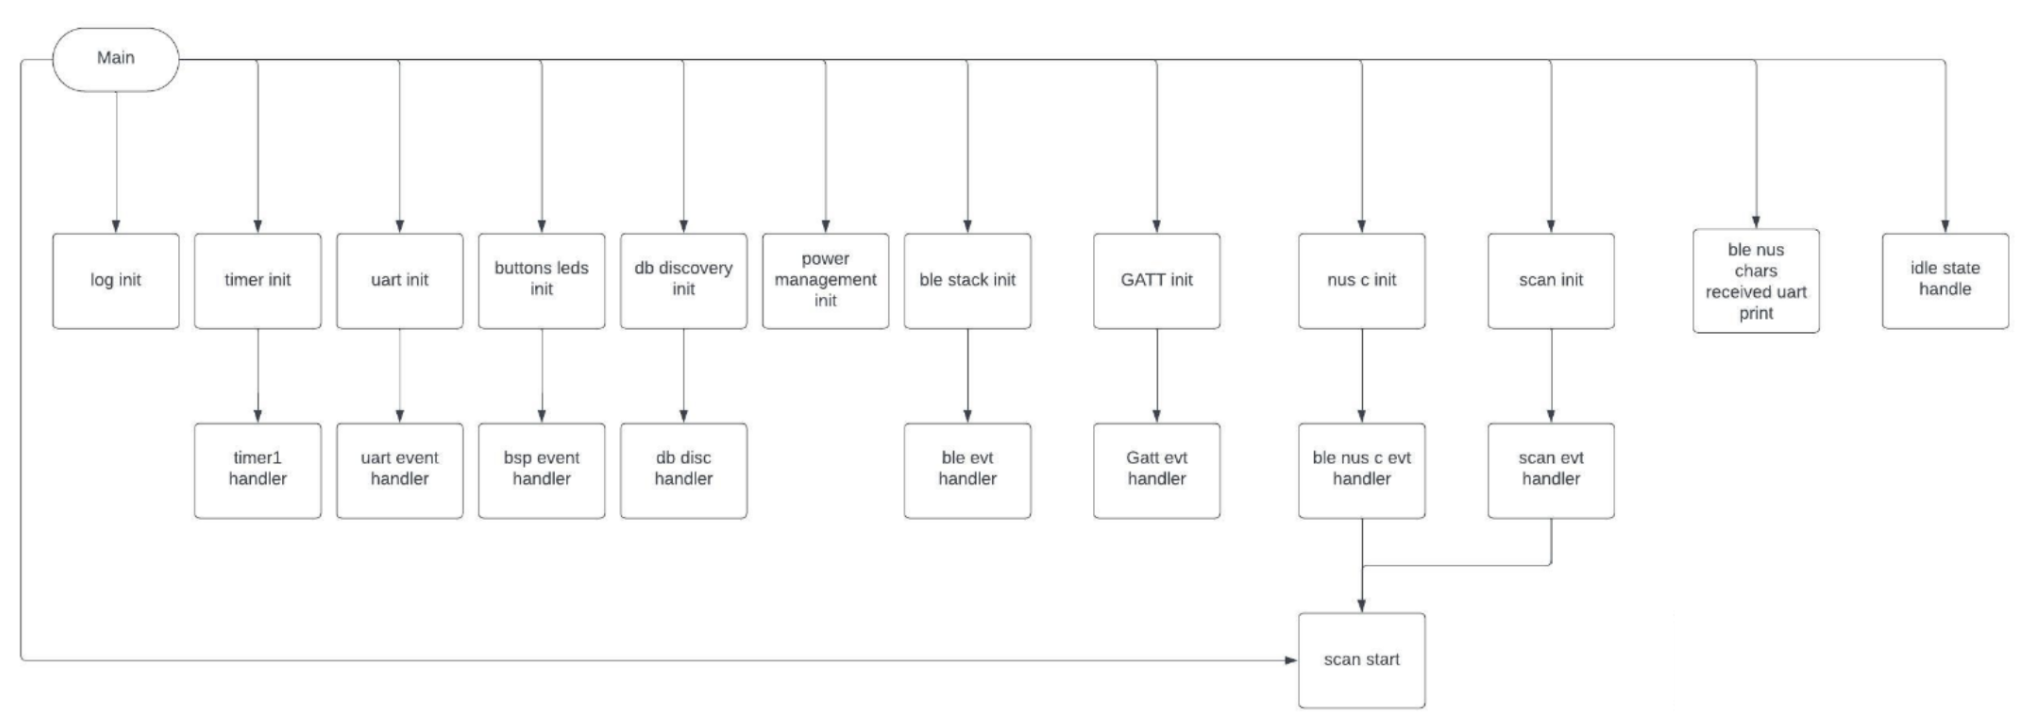
\includegraphics[scale=0.3]{Previous Implementation/Screenshot 2024-08-15 at 11.01.10.png}
	\centering
    \label{prev_5}
    \caption{Offline Receiver Code}
\end{figure}

\subsection*{Offline Receiver Code}

Some functions in the receiver code are common with those in the transmitter, such as the \texttt{log\_init} function, used in both receiver and transmitter in the same way. The \texttt{timer\_init} function is also similar, differing in the number of timers initialized (one in the receiver). The receiver’s timer computes the time elapsed in the data receiving process, equivalent to the transmitter’s timer2. Functions \texttt{power\_management\_init} and \texttt{ble\_stack\_init} are identical for both. Some functions are similar but differ due to the different central/peripheral roles, particularly:
\begin{itemize}
    \item \textbf{GATT Init:} \texttt{nrf\_ble\_gatt\_att\_mtu\_periph\_set} is replaced by \texttt{nrf\_ble\_gatt\_att\_mtu\_central\_set}.
    \item \textbf{GATT Event Handler:} The connection handle check is not present in the receiver code since the peripheral can be connected to more than one central device.
\end{itemize}

Other functions are different or not present in the transmitter code and are explained below.

\textbf{UART Initialization}: this function initializes the UART, which lets the central device communicate with the external unit. First, the communication parameters are defined, setting the pin number for the UART receive (RX), UART transmit (TX), UART Ready To Send (RTS), and UART Clear To Send (CTS) lines. In this case, they are 8 and 6 for RX and TX, and 5 and 7 for RTS and CTS, respectively. Hardware flow control is disabled through the \texttt{APP\_UART\_FLOW\_CONTROL\_DISABLED} macro, and parity checking is disabled, meaning no parity bit will be used for error checking. The baud rate is set to 115200 bits per second. Finally, the \texttt{APP\_UART\_FIFO\_INIT} function makes the parameters effective. This setup ensures the UART is correctly configured and ready to handle data transmission and reception with FIFO buffers and appropriate event handling.

\textbf{UART event handler}: this function is responsible for receiving commands from the external unit. Within this function, a switch statement manages different cases. The first case handles the reception of new data through UART. Commands from the external unit are received as sequences of characters in the UART\_event\_handler function. Upon receiving a new character via \texttt{app\_uart\_get}, it is stored in \texttt{data\_array} at position \texttt{index}, which is then incremented. Once a character is saved, it checks if the character is equal to '\textbackslash n' and if \texttt{index} exceeds \texttt{m\_ble\_nus\_max\_data\_len}. If true, it indicates the command is fully received, and the string is sent to the peripheral device via the function \texttt{ble\_nus\_c\_string\_send}. \texttt{m\_ble\_nus\_max\_data\_len} represents the maximum data length in bytes that can be transmitted by the Nordic UART service module, specifically BLE\_GATT\_ATT\_MTU\_DEFAULT minus the two headers OP Code and Handle Length, which is 23 minus 3 bytes. After sending the string, \texttt{index} is reset to zero. The other cases handled in this function are \texttt{APP\_UART\_COMMUNICATION\_ERROR} and \texttt{APP\_UART\_FIFO\_ERROR}, which report communication and FIFO module errors to the user through log messages.

\textbf{Buttons LEDs Initialization}: this function initializes buttons and LEDs using two functions: \texttt{bsp\_init} for LEDs and \texttt{bsp\_btn\_ble\_init} for buttons.


\textbf{BSP Event Handler}: this function handles events from the Board Support Package (BSP) module using a switch-case statement. The sleep event calls \texttt{nrf\_pwr\_mgmt\_shutdown} with \texttt{NRF\_PWR\_MGMT\_SHUTDOWN\_GOTO\_SYSOFF} to put the system into a low-power system-off state. The disconnect event calls \texttt{sd\_ble\_gap\_disconnect} to terminate the Bluetooth connection, providing the connection handle and reason for disconnection.

\textbf{Database Discovery Initialization}: this function initializes the Database Discovery (DB) module using \texttt{ble\_db\_discovery\_init}, which handles service discovery on GATT servers.

\textbf{DB Discovery Handler}: this function is a callback function to handle events from the database discovery module, forwarding events to respective services based on discovered UUIDs.

\textbf{BLE Event Handler}: this function handles BLE events with differences between transmitter and central code. For connection events, changes LED behavior and assigns the connection handle using \texttt{ble\_nus\_c\_handles\_assign}. Additional tasks include starting service discovery with \texttt{ble\_db\_discovery\_start}. PHY settings are not set in central code as it responds to PHY update requests from the peripheral. Disconnect events log disconnection without changing the connection handle. Common cases include security parameter requests, PHY update requests, and GATTC/GATTS event timeouts. Unique cases not present in the transmitter's \texttt{ble\_evt\_handler} are BLE\_GAP\_EVT\_TIMEOUT for GAP operation timeouts and BLE\_GAP\_EVT\_CONN\_PARAM\_UPDATE\_REQUEST for peripheral-initiated connection parameter updates.

\textbf{NUS Central Initialization}: this function initializes the Nordic UART Service (NUS) for the central role using specific functions.

\textbf{BLE NUS Central Event Handler}: this function handles data reception from the peripheral through NUS. Uses a switch statement to manage cases:
\begin{itemize}
    \item Completes NUS discovery, assigns connection handle, and enables notifications for data reception.
    \item Manages arrival of data packets from peripheral. Increments \texttt{received\_bytes} and computes throughput based on the time elapsed since the first packet.
    \item Saves packet data into \texttt{senseback\_buff}. Computes throughput when the last two bytes of a packet are 255.
    \item Updates \texttt{senseback\_buff\_length} and checks for buffer overwrite.
    \item Handles disconnection events by calling \texttt{scan\_start} to initiate a new connection.
\end{itemize}
Throughput is computed using the formula: \(\text{throughput} = \frac{\text{number of bits received from peripheral}}{\text{time elapsed in data receiving process}}\). This throughput computation differs from that in the transmitter code by focusing solely on data receiving time, making it more reliable for communication speed analysis.



\textbf{Scan start}: this function initiates the scan process by performing two actions. Firstly, it starts the board scanning using \texttt{nrf\_ble\_scan\_start}. Secondly, it sets the LEDs to indicate that the board is in the scanning phase, with \texttt{LED1} specifically configured to start blinking.

\textbf{Scan init}: this function serves two main purposes: setting scanning parameters and enabling scan filters. It sets two scanning parameters:
\begin{itemize}
    \item \texttt{connect\_if\_match} is set to \texttt{true}, allowing the scanning process to automatically attempt to establish a connection.
    \item \texttt{conn\_cfg\_tag} is set to \texttt{APP\_BLE\_CONN\_CFG\_TAG}, which refers to the BLE stack configuration tag. In this case, the value is set to 1, indicating the configuration with handle one.
\end{itemize}
After initializing BLE scanning, filters are configured and enabled. The scanning module filter type is \texttt{SCAN\_UUID\_FILTER}, ensuring that only advertisements from devices offering the NUS service are reported.


\textbf{Scan event handler}: this function handles events from the Scanning Module, addressing three specific events:
\begin{itemize}
    \item An error occurring during the connection process retrieves the error code from the event parameters.
    \item Successful establishment of a connection retrieves the connected event parameters and logs the address of the connected peer.
    \item Timeout event during the scan process logs a message indicating the scan has timed out and calls \texttt{scan\_start} to restart the scanning process.
\end{itemize}

\textbf{BLE NUS Chars Received Parameters Print}: this function is continuously called in the main program until there is no data overwrite in the circular buffer \texttt{senseback\_buff}. It handles sending data to the external unit via UART. It takes as inputs each newly stored row in \texttt{senseback\_buff} and the length of the new packet. Data are sent via UART using \texttt{app\_uart\_put} until all data are sent or a memory resource error occurs. Error checking mechanisms are implemented to notify the user of the position in the packet where an error occurred. Additionally, the function allows for flagging \texttt{ECHOBACK\_BLE\_UART\_DATA}. In this case, data sent via UART to the external unit are also sent back to the peripheral, providing an additional transmission verification.

\textbf{Idle State Handle}: this function is also present in the transmitter code, but for what regards the receiver it is much simpler. This is called each time code is in idle state. What is does it to handle any pending log operations, then it come back to sleep until next event occurs.

\begin{figure}[H]
	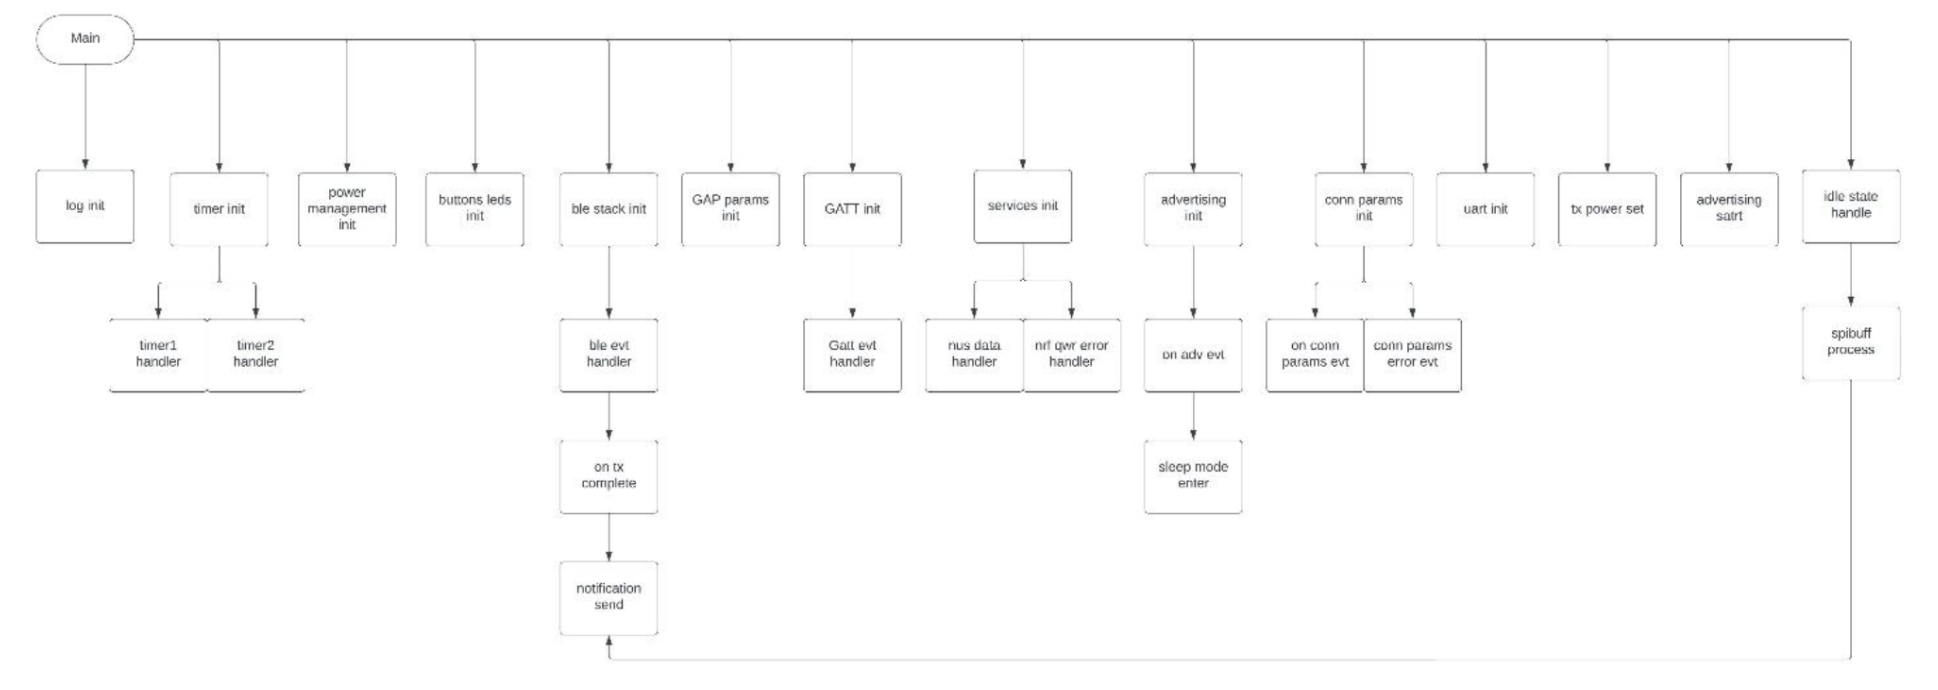
\includegraphics[scale=0.3]{Previous Implementation/Screenshot 2024-08-15 at 11.01.21.png}
	\centering
    \label{prev_6}
    \caption{Online transmitter code}
\end{figure}

\subsection{Online transmitter code}

The online transmitter code is quite similar to the offline one, it just presents some small differences to guarantee the previously described different intended behaviour. The flow chart of this code is shown in Figure 6. The differences between the two codes inside the functions will be underlined below. 
Timer1 handler: This function remains responsible for data generation but differs from the offline case in several aspects. Firstly, although the generated \texttt{uint16\_t} value \texttt{CNT} still increments step-wise, an upper limit of 65530 is set. Upon reaching this value, \texttt{CNT} resets and data generation resumes from zero. In offline tests, \texttt{CNT} would not exceed 16198 to communicate 32400 bytes, whereas online tests allow \texttt{CNT} to potentially grow endlessly. Secondly, in the online code, \texttt{timer1\_handler} is not responsible for ending communication; instead, transmission concludes upon receiving the STOP command from the user.

\subsection*{Notification Send}
This function is nearly identical to its offline counterpart, with a small difference in the condition for determining the end of communication. In addition to checking if the last two bytes sent are 255, it verifies if transmission is still ongoing by examining the boolean variable \texttt{transmission}. If \texttt{transmission} is false, indicating the user sent the command STOP, this ensures the last two bytes 255 signal the transmission's end.

\subsection*{NUS Data Handler}
This function manages reception of commands from the external unit, particularly handling the STOP command differently. Upon receiving this command, \texttt{timer1} is disabled to halt the data transmission process. Additionally, the value 65535 is placed into the ring buffer, and \texttt{transmission} is set to false. These steps are placed differently from the offline code to accommodate behavior variations between tests. In offline tests, these actions were inside \texttt{timer1\_handler} to end communication upon data generation completion. In online tests, communication ends only upon user command.

\subsection*{SpiBuff Process}
This function processes data similarly to the offline case until reaching the last packet. In the online code, it does not check if the remaining number of data to be sent is less than 244. Instead, it verifies if there is still data in the ring buffer and if transmission is false, indicating receipt of the STOP command. If true, it processes the final stop as before.

\subsection*{Additional Functions}
Two functions added to the online receiver code that are not in the offline version:
\begin{itemize}
    \item \texttt{buttons\_leds\_init} and \texttt{uart\_init}, previously explained in the offline receiver code section. These are not strictly necessary for the online transmitter code's purposes.
\end{itemize}

\begin{figure}[H]
	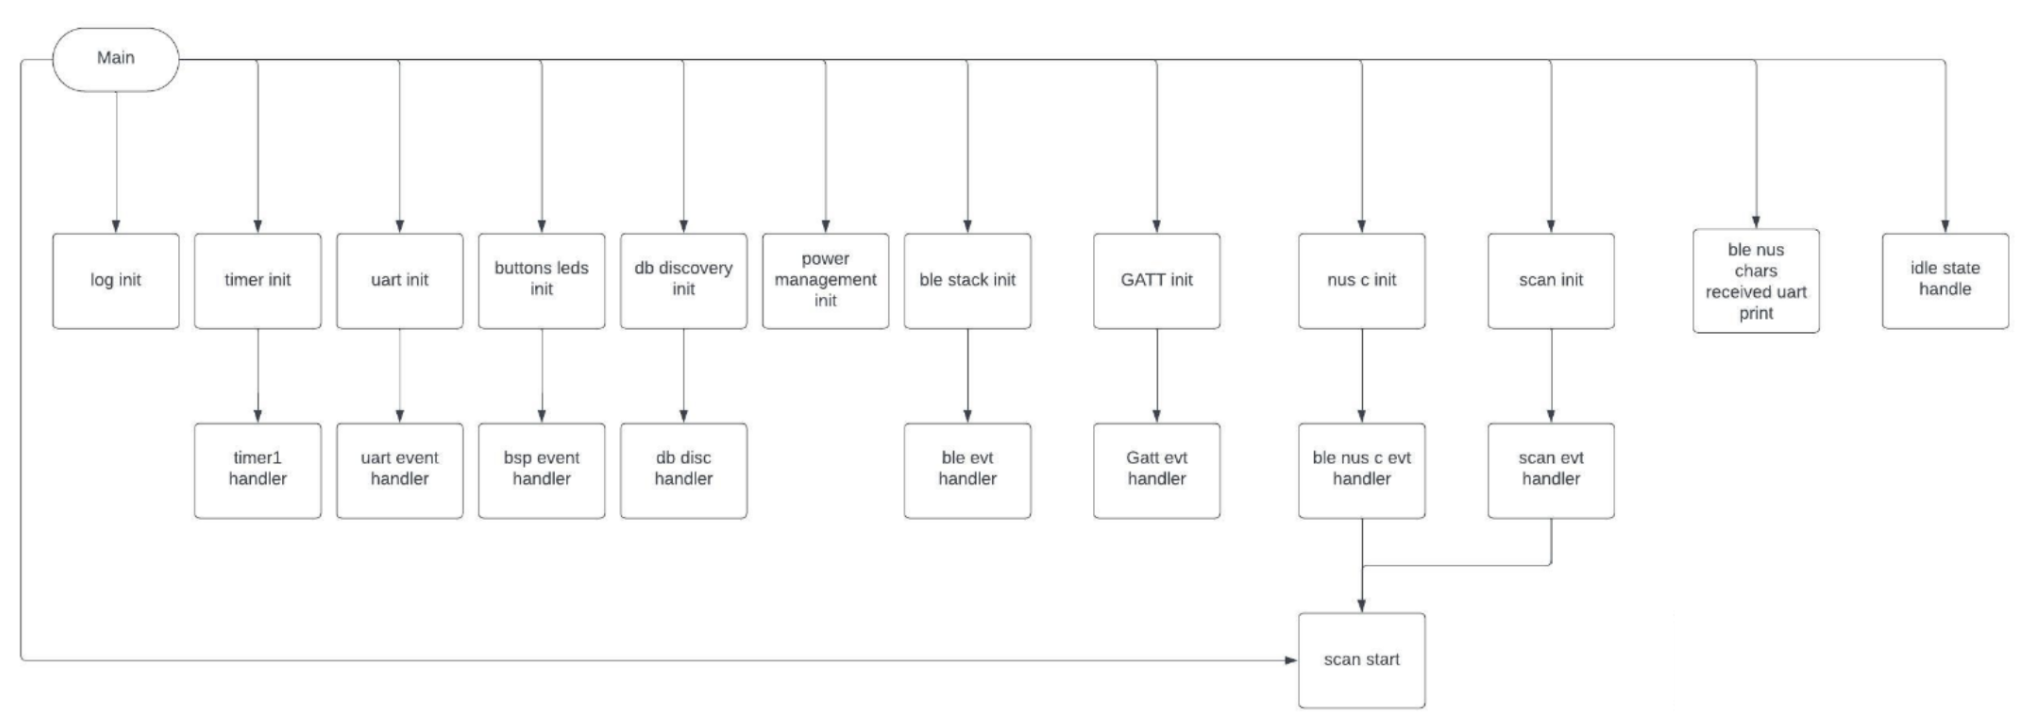
\includegraphics[scale=0.3]{Previous Implementation/Screenshot 2024-08-15 at 11.01.10.png}
	\centering
    \caption{Additional functions}
    \label{prev_7}
\end{figure}

\subsection{Online Receiver Code}
For the online receiver code, the flow chart mirrors Figure 5. However, some functions have minor differences to accommodate the online test's different behavior:
\begin{itemize}
    \item \texttt{Uart event handle}: Similar to the offline receiver case, but the received UART command is stored and checked locally. If it matches \texttt{"STOP\textbackslash n"}
    , \texttt{end\_transmission} is set to true, signaling the receiver to end communication.
    \item \texttt{Ble nus c evt handler}: Similar to the offline case, with an additional condition to check the end of transmission. Besides checking the last two values being 255, it verifies \texttt{end\_transmission} is true. This ensures the receiver recognizes the last two 255 values after the user enters the STOP command, concluding data reception.
\end{itemize}

\subsection{Sniffer Code}
The sniffer provides real-time monitoring of transmission parameters such as PHY, ATT MTU, and protocol, and also tracks the number of retransmissions during tests. To utilize it:
\begin{itemize}
    \item A software tool is needed, available for the nRF52840 dongle when in debug mode. Specifically, \texttt{sniffer\_nrf52840dongle\_nrf52840\_4.1.1.hex} is used.
    \item Cross-platform development software like nRF Connect for Desktop is required, with the "Programmer" app used to execute the code on the sniffer.
    \item Once the sniffer is connected to the PC in debug mode, the code can be executed, enabling it to function with Wireshark for analysis.
\end{itemize}


\subsection{Bonding}

The pairing procedure may involve an additional phase, referred to as Phase 3, in cases where bonding is required. The term "bonding" refers to connections where it is necessary to avoid restarting the pairing process from scratch each time a new connection is established. This is particularly relevant when devices enter standby mode and need to restore communication after some time. If bonding is required, it is possible to exchange different keys compared to those generated during the pairing process, specifically Long-Term Keys (LTK). During Phase 3, it is also possible to share additional optional keys such as the Identity Resolving Key (IRK), which is useful for resolving private addresses to allow devices to recognize each other even with random resolvable addresses, or the Connection Signature Resolving Key (CSRK), which can be used to authenticate data in unencrypted connections to verify that the data received comes from the intended device. 

\begin{figure}[h]
\centering
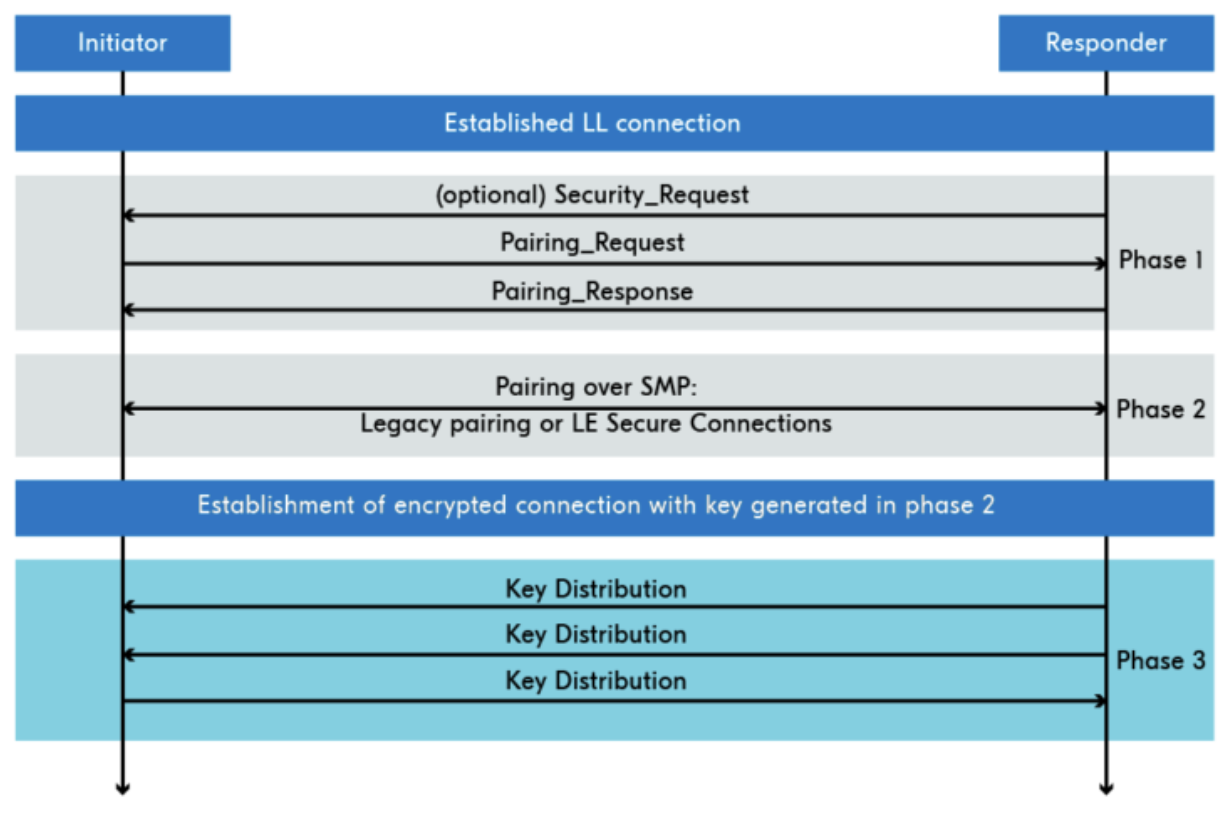
\includegraphics[scale=0.7]{Bluetooth_Security/4.png}
\label{bluetooth_sec_4}
\caption{Bluetooth bonding table}
\end{figure}

\subsection{Legacy Pairing and Low Energy Secure Connection (LE-SC)}

Since the introduction of Bluetooth Low Energy version 4.2, a further level in mode 1 has been added to the initial three. This new level is named Low Energy Secure Connection (LE-SC), while the previously described pairing procedure is referred to as legacy authentication. This new level is an addition rather than an alternative to the previous levels. LE-SC provides a higher level of security compared to legacy pairing, as the short-term key (STK) generated during legacy pairing has been found to be susceptible to attacks, particularly in cases where the "Just Works" procedure was used. Even with passkey entry, the passkey exchange can be sniffed, allowing a hacker to potentially compromise the STK. Out of band is somewhat more secure, but its safety depends on the security of the secondary channel.

For these reasons, legacy pairing has become obsolete, and LE-SC should be preferred when supported. The main idea behind LE-SC is the use of Elliptic Curve Diffie-Hellman (ECDH) instead of STK. ECDH allows devices to select a private key without sharing it over the air, ensuring that the password can be agreed upon without the risk of interception. Only a public key is exchanged during the process.

\begin{figure}[H]
    \centering
    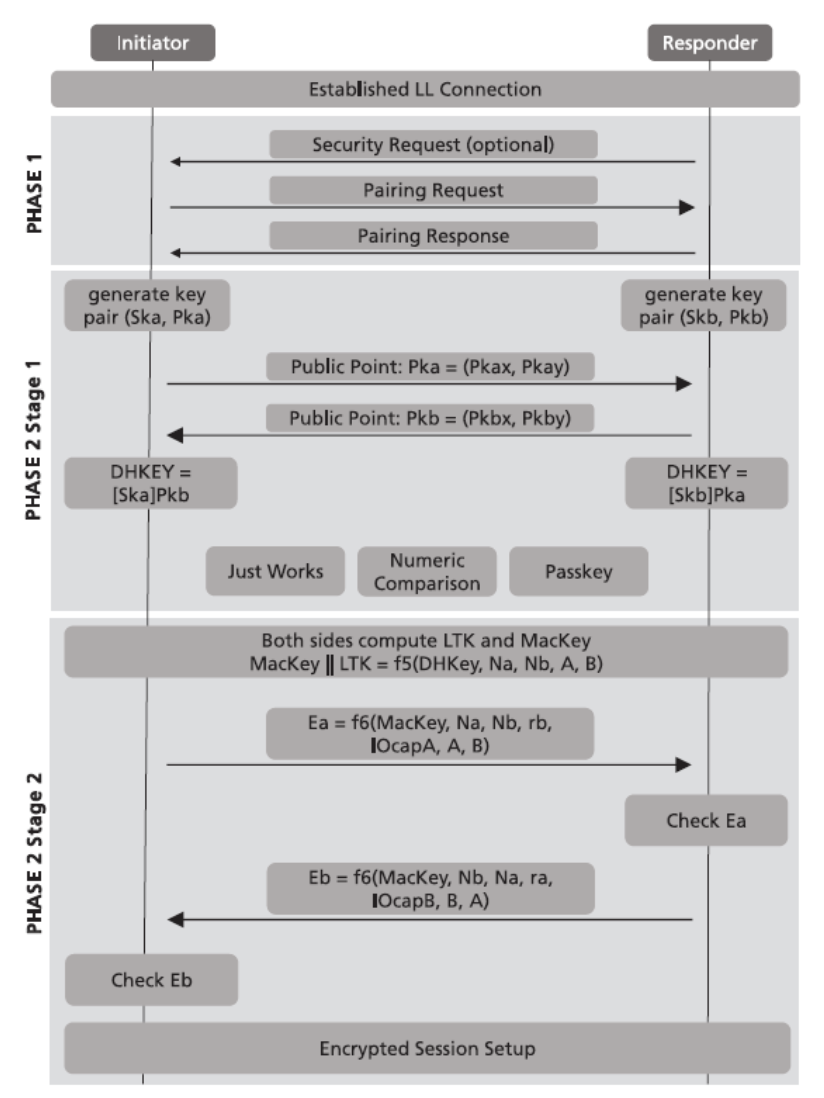
\includegraphics[scale=0.7]{Bluetooth_Security/5.png}
    \caption{Bluetooth LESC table \cite{PairingProcess}}
    \label{bluetooth_sec_5}
\end{figure}

Figure 3.15 shows the pairing procedure for a Low Energy Secure Connection. As illustrated, the procedure consists of two distinct phases. The first phase is almost equivalent to Phase 1 in the legacy pairing process, with one notable difference: a flag is added to indicate whether the devices are capable of performing the LE-SC procedure, as indicated in the pairing response. 

Phase 2 is divided into two stages. The first stage begins when both devices generate a random private key (Ska or Skb) and a public key (Pka and Pkb). The public keys are exchanged, and a common key (DHKEY) is computed from these values. The subsequent steps depend on the chosen association mode. Specifically, LE-SC supports three different association modes: Just Works, Numeric Comparison, Passkey Entry, and Out of Band.

\textbf{Just Works} is the association mode that offers the lowest level of security, as no authentication is required, even though LE-SC makes this mode more secure. This mode does not protect against man-in-the-middle (MITM) attacks. Both Just Works and Numeric Comparison association modes are depicted in Figure 3.16.

\begin{figure}[H]
    \centering
    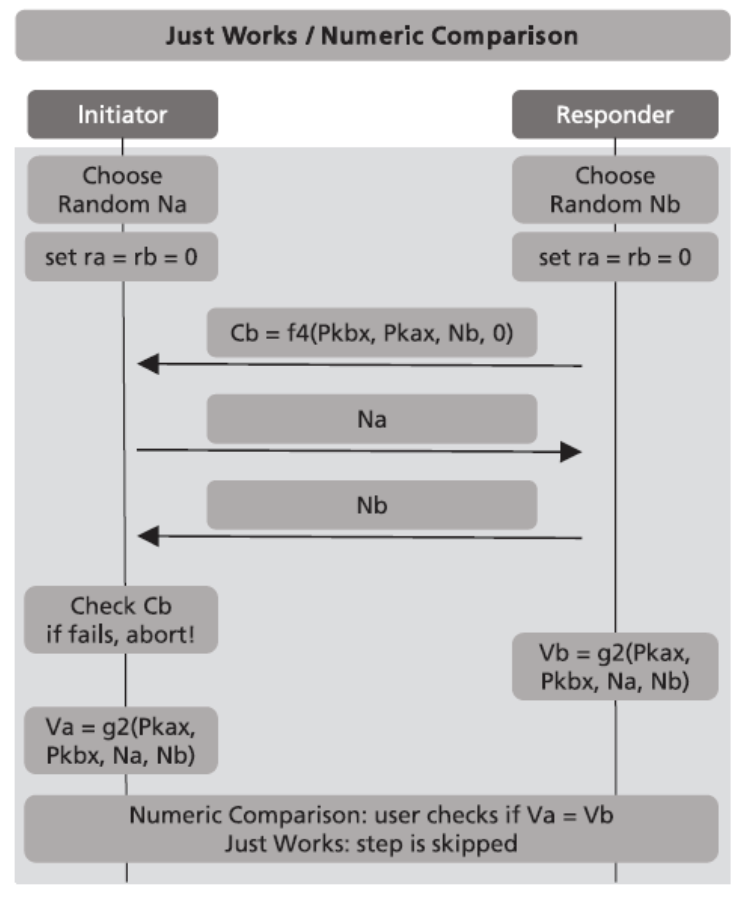
\includegraphics[scale=0.7]{Bluetooth_Security/6.png}
    \caption{Bluetooth legacy table \cite{casarSurveyBluetoothLow2022}}
    \label{bluetooth_sec_6}
\end{figure}

The procedures start when peripheral and central devices generate random numbers (Na and Nb). Once this step is complete, the central device generates a new value Cb, based on the previously generated values Pkax and Pkbx along with the new value Nb. This value Cb is then sent to the peripheral device. Both devices share their generated random values Na and Nb, allowing the peripheral device to verify the correctness of the received value Cb. If Cb is incorrect, the procedure is aborted, which can happen if values Pkax, Pkbx, or Nb change during the exchange, such as during a hacker attack. If the Just Works procedure is chosen, the association process ends at this stage. If Numeric Comparison is chosen, both devices display a random 6-digit number (Va and Vb), and the user must confirm that the numbers are identical. Numeric Comparison introduces additional protection against MITM attacks, ensuring that none of the random numbers have been altered.

Another association mode supported by LE-SC is the Passkey Entry, detailed in Figure 3.17.

\begin{figure}[H]
    \centering
    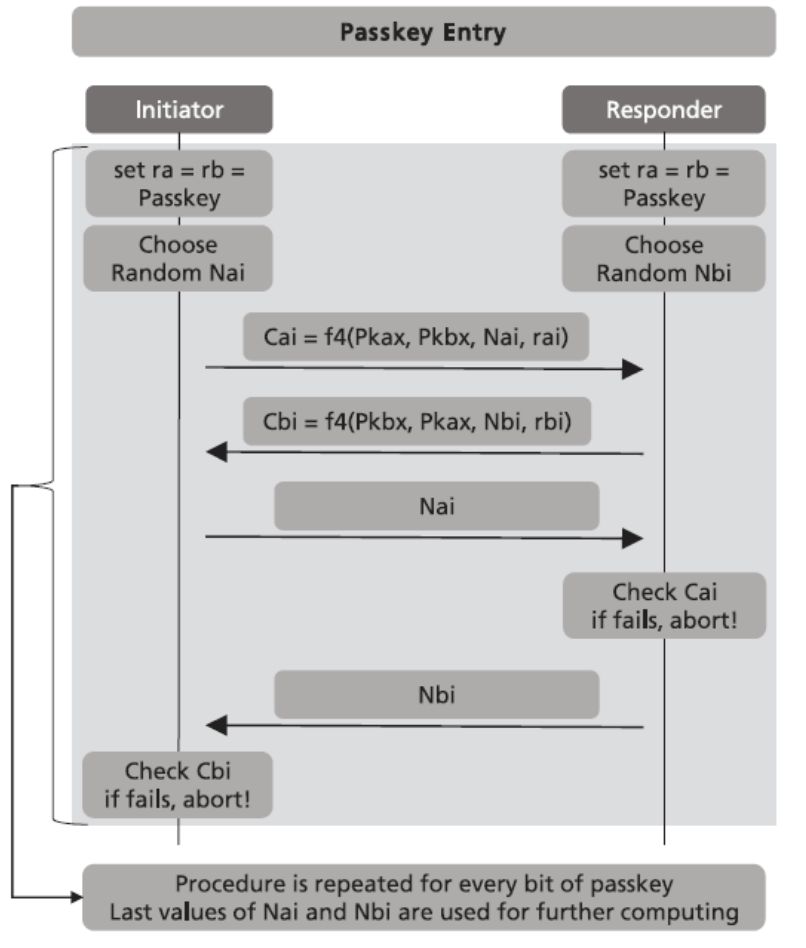
\includegraphics[scale=0.7]{Bluetooth_Security/7.png}
    \caption{Passkey entry \cite{casarSurveyBluetoothLow2022}}
    \label{bluetooth_sec_7}
\end{figure}

The Passkey Entry procedure requires that at least one of the devices has keyboard capabilities. Depending on whether one or both devices have input capabilities, the procedure may vary slightly. Specifically, the user may be asked to enter the same value on both devices, or a randomly generated value may be displayed on one device, which must then be entered into the other device. This process is repeated for each bit of the password. Each iteration generates a commitment value Cb, based on the ECDH values Pkax and Pkbx, along with the random values Na and Nb and the last bit of the password (ra and rb). To prevent MITM attacks, the central device shares its random value Na with the peripheral device to verify its commitment value Ca, and this step is repeated with roles reversed. If a mismatch occurs, the procedure is aborted. If no errors occur, LTK and MACkey are generated. A MITM attacker would need to alter each bit of the password for each iteration, which is mitigated by the high length of Na and Nb values. Following Bluetooth SIG requirements, each password is used only once, preventing reuse attacks. The values Pkax and Pkbx are included in the commitment value to prevent separate ECDH exchanges and password entries by a potential attacker.

The final association mode supported by LE-SC is Out of Band (OOB), as shown in Figure 3.18.

\begin{figure}[H]
    \centering
    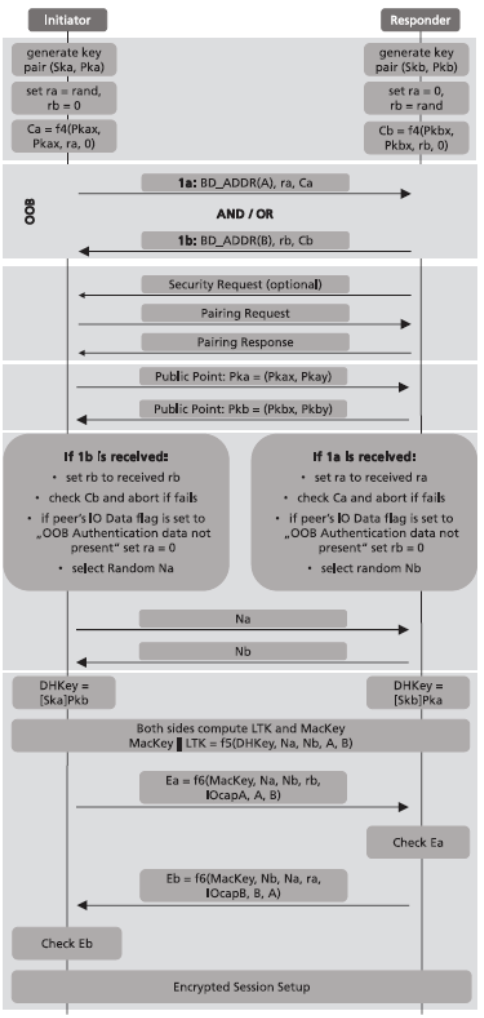
\includegraphics[scale=0.7]{Bluetooth_Security/8.png}
    \caption{Bluetooth legacy table \cite{casarSurveyBluetoothLow2022}}
    \label{bluetooth_sec_8}
\end{figure}

To indicate that OOB association mode is required, the OOB data flag must be set to true for each device. This indication occurs when the devices initiate the pairing procedure, and the OOB connection must be established before this moment. OOB can be performed in various ways, and the pairing procedure might be triggered by the OOB procedure. Both devices generate public and private ECDH keys and select random values ra and rb. Commitment values Ca and Cb are computed as in the previously explained association modes. The OOB connection is then established, which varies based on the devices' capabilities. If both devices can receive and transmit data, values 1a and 1b are exchanged; otherwise, only one device exchanges data. After completing the OOB data transfer, BLE communication is established, and the pairing procedure proceeds as before, with flags set to indicate authentication requirements. If OOB data exchange occurs, the commitment value is verified. If mismatches are found, the pairing procedure is aborted. The OOB data flag indicates successful data exchange. OOB is considered secure enough for legacy pairing and is recommended for LE-SC, provided the OOB channel is secure.

All association modes result in the generation of two random values Na and Nb. Phase 2, Stage 2 then begins, where LTK and MACkey are generated using Na, Nb, device addresses, and public and private keys from the chosen association mode. This final value links all previous procedures and prevents attacks. Confirmation values Ea and Eb are computed using Mackey, Na, Nb, ra, rb, device BLE addresses, and keyboard/display capabilities. These values are shared and checked without directly exchanging the DHkey. If no errors occur, LTK is generated, and the pairing procedure is completed. Unlike legacy pairing, LTK generation is not an optional consequence of STK but is automatically generated after the process. LTK can be discarded if bonding is not required, or stored for future use. In LE-SC, if bonding is requested, IRK and CSRK values may also be used.
When switching roles, if a mismatch occurs, the procedure is immediately aborted. If no errors are found during each iteration, the Long-Term Key (LTK) and the Media Access Control key (MACkey) are generated. The MACkey is used for media access control. To prevent a potential man-in-the-middle (MITM) attacker from exploiting the password, each bit of the password must be changed in every iteration. This high complexity prevents such attacks, as the length of Na and Nb values is significant. According to Bluetooth SIG requirements, each password must be used only once, which prevents an attacker from gaining information from an aborted procedure. Additionally, to prevent an attacker from performing independent ECDH exchanges and password entries, the values Pkax and Pkbx are included in the commitment value.

\subsection{Encryption}

Once the pairing procedure concludes, the devices have generated the LTK or STK, depending on the procedure chosen and whether bonding is enabled. These keys are used to encrypt the connection. The encryption procedure is shown in Figure \ref{bluetooth_sec_9}.

\begin{figure}[H]
    \centering
    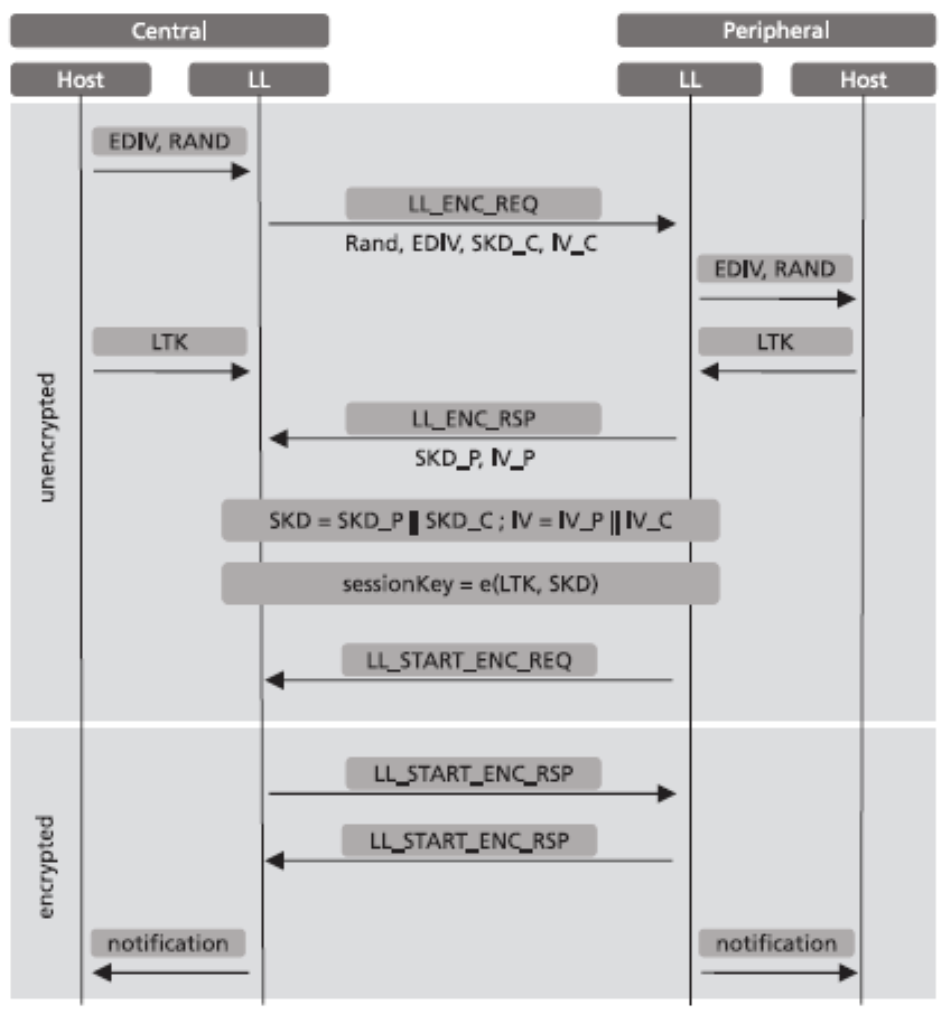
\includegraphics[scale=0.7]{Bluetooth_Security/9.png}
    \caption{Encryption \cite{casarSurveyBluetoothLow2022}}
    \label{bluetooth_sec_9}
\end{figure}

If a long-term key (LTK) has been generated, the values EDIV and RAND are shared between the devices to reconstruct the LTK. These values act as identifiers to recover the LTK. Specifically, the central device shares its EDIV and RAND values with the peripheral device, which can retrieve its values from its database. If only the pairing procedure is performed and STK and LTK are not present, these fields are set to zero. 

Both devices then generate and share two random numbers, each 128 bits long: \( \text{SKD}_C \), \( \text{IV}_C \) for the central device and \( \text{SKD}_P \), \( \text{IV}_P \) for the peripheral device. These represent the session key diversifiers and initialization vectors. The values for central and peripheral devices are concatenated through a link layer encryption request (LL\_ENC\_REQ). After concatenation, the session key is computed using the AES-128 algorithm, incorporating the newly generated SKD values and the previously generated STK/LTK. This session key is then used for encryption.


\begin{figure}[H]
    \centering
    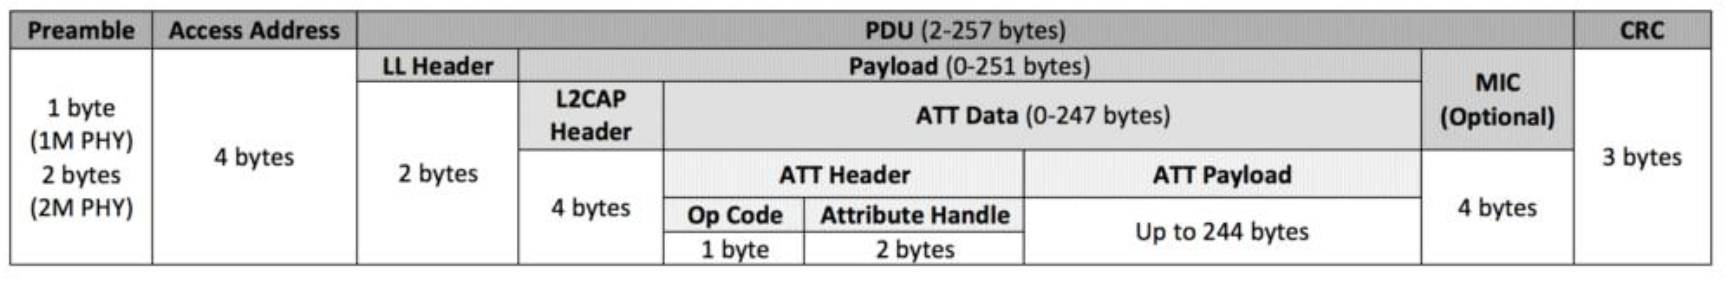
\includegraphics[scale=0.5]{Bluetooth_Security/10.png}
    \caption{BLE packet structure \cite{afanehBluetoothSpeedHow2023}}
    \label{bluetooth_sec_10}
\end{figure}

The encryption process begins by adding a message integrity check (MIC) field to the BLE packet, as shown in Figure 3.20. The MIC field is 4 bytes long. Encryption is applied to the PDU and the MIC field. As illustrated in Figure 3.20, not the entire BLE packet is encrypted; only the payload and MIC field are encrypted, as they may contain sensitive data. The remaining parts, including headers, remain unencrypted. The unencrypted portions of the BLE packet contain minimal, generally non-sensitive information.

\subsection{Man-in-the-Middle Attack}

The implementation of security measures aims to protect against man-in-the-middle (MITM) attacks. A MITM attack allows the attacker not only to intercept packets using a sniffer but also to potentially compromise the reliability of the BLE connection. Specifically, in Bluetooth Low Energy, the attacker must impersonate both the receiver and transmitter devices, causing legitimate central and peripheral devices to connect to the malicious devices and exchange data. Protection against such attacks is only guaranteed if both legitimate devices require MITM protection and possess input/output capabilities. Otherwise, no protection is assured.

\subsection{Modes 2 and 3}

Modes 2 and 3 offer different security features in Bluetooth Low Energy. Mode 2 is based on connection-based data signing, which ensures that data remains intact and reliable throughout the process. This is achieved by generating a unique identifier (starting from CSRK) for each sent packet. This procedure ensures that data has not been altered during transit and that the data is authenticated, meaning it originates from the expected device. As shown in Table 3.11, Mode 2 is divided into two levels:

\begin{itemize}
    \item \textbf{Level 1}: Provides no data authentication. Pairing is performed without the need for input/output capabilities, typically using the Just Works association mode, with no MITM protection.
    \item \textbf{Level 2}: Includes other association modes such as Out of Band, Numeric Comparison, or Passkey Entry, which offer higher levels of security.
\end{itemize}

The connection data signing procedure is as follows:
\begin{enumerate}
    \item Pairing procedure is performed, and CSRK is generated and exchanged.
    \item The transmitter device prepares a data packet and generates a signature using CSRK, which includes a MAC and a counter that increments with each new data packet.
    \item The BLE packet and its corresponding signature are sent from the transmitter to the receiver device.
    \item The receiver device reconstructs the signature using its CSRK and data counter. If the signatures from the receiver and transmitter do not match, the receiver cannot be certain of the data's reliability. A mismatch in the counter value indicates potential manipulation by an attacker.
\end{enumerate}

Mode 3 is used in broadcast connections requiring encryption and is divided into three levels:
\begin{itemize}
    \item \textbf{Level 1}: Provides no security and does not implement encryption.
    \item \textbf{Level 2}: Data is encrypted, but there is no authentication process, providing a moderate level of security.
    \item \textbf{Level 3}: Data is both encrypted and authenticated using a Broadcast Code. This feature, implemented in BLE version 5.4, uses the CCM encryption algorithm for both encryption and authentication of Advertisement Data (AD data). The Key Material, used for encryption, is stored in the peripheral device and shared with the GATT client.
\end{itemize}


\section{Hardware}

For what regards the experimental setup, some specific components are chosen. Firstly, the two boards which communicate through Bluetooth Low Energy are two nrf52dk boards. These are equipped with a nRF52832 chip, which is part of the Nordic Semiconductor’s nRF52® Series of System-on-Chip (SoC) devices. This series is the one taken into consideration due to its versatility, giving the user the ability to choose which components are the best fit for the intended usage, its documentation, and its support features during the development phase of the project. The main features of this chip are reported in Table 1 below:

\begin{figure}[H]
    \centering
    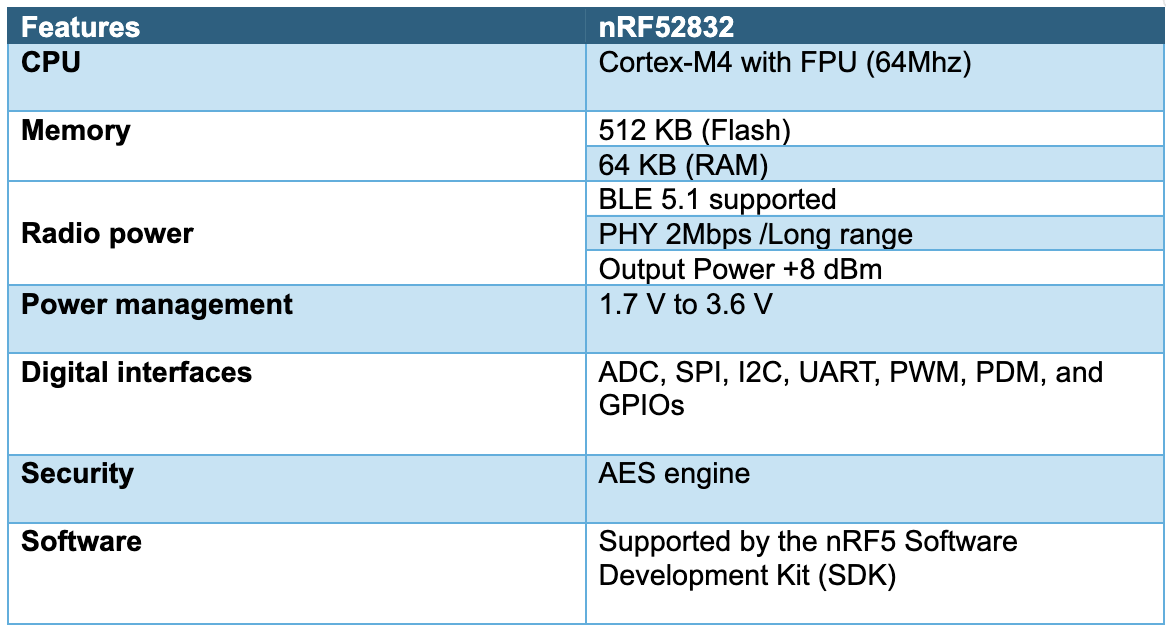
\includegraphics[width=0.6\textwidth]{Materials/figure1}
    \label{materials_1}
    \caption{Hardware table}
\end{figure}

The memory sizes are equivalent to the ones of the actual Senseback device, making the development of the firmware reliable. A picture of a nrf52dk board is shown in the figure above.

\begin{figure}[H]
    \centering
    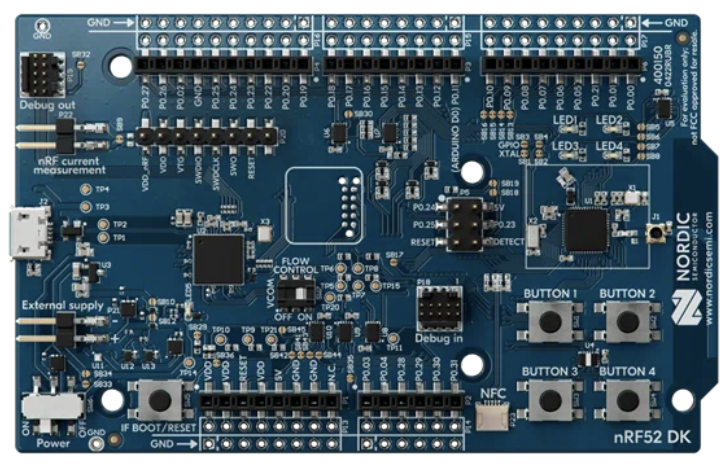
\includegraphics[width=0.6\textwidth]{Materials/figure2}
    \label{materials_2}
    \caption{NRF52DK board}
\end{figure}

Instead, for what regards the sniffer, a nRF52840 MDK USB Dongle has been chosen.

\begin{figure}[H]
    \centering
    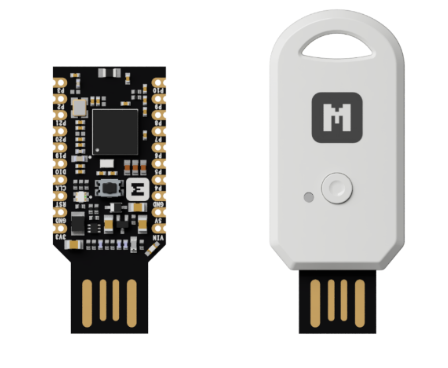
\includegraphics[width=0.6\textwidth]{Materials/figure3}
    \label{materials_3}
    \caption{USB Dongle}
\end{figure}

This dongle supports Bluetooth Low Energy version 5, is equipped with a 32-bit ARM Cortex-M4 CPU with FPU, and provides robust processing power for handling complex tasks and algorithms. It also features 256 KB of RAM and 1 MB of Flash memory, which are ample for most applications and development needs.

Finally, the last component is the one used to measure charge and current consumption absorbed by the device during the communication. For this purpose, the Power Profiler Kit II (PPK2) has been chosen.

\begin{figure}[H]
    \centering
    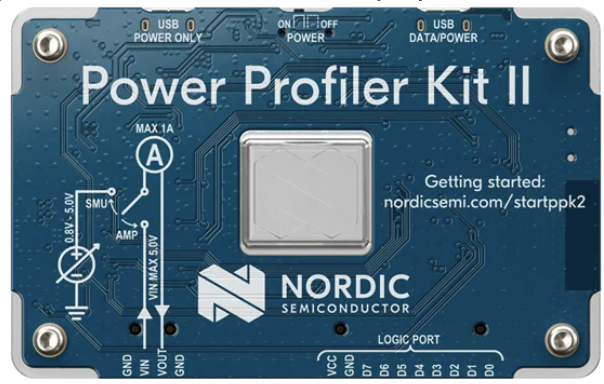
\includegraphics[width=0.6\textwidth]{Materials/figure4}
    \label{materials_4}
    \caption{Power profiler kit}
\end{figure}

This tool can both measure instantaneous current consumption and supply the device under test. It is designed by Nordic Semiconductor®, but it can also be useful when used with third-party tools. It presents two different modalities: ampere meter mode and source meter mode. For the first mode, the board should be supplied by further external alimentation, which is not required when using the source meter mode, where the board could be powered through the PPK2 itself. The hardware is managed by one of the specific apps in nRF Connect for Desktop: the Power Profiler app, which allows the user to set the intended voltage used to supply the board and to monitor the current consumption in real-time. The table reported below illustrates the main characteristics of the Power Profiler Kit II.

\begin{figure}[H]
    \centering
    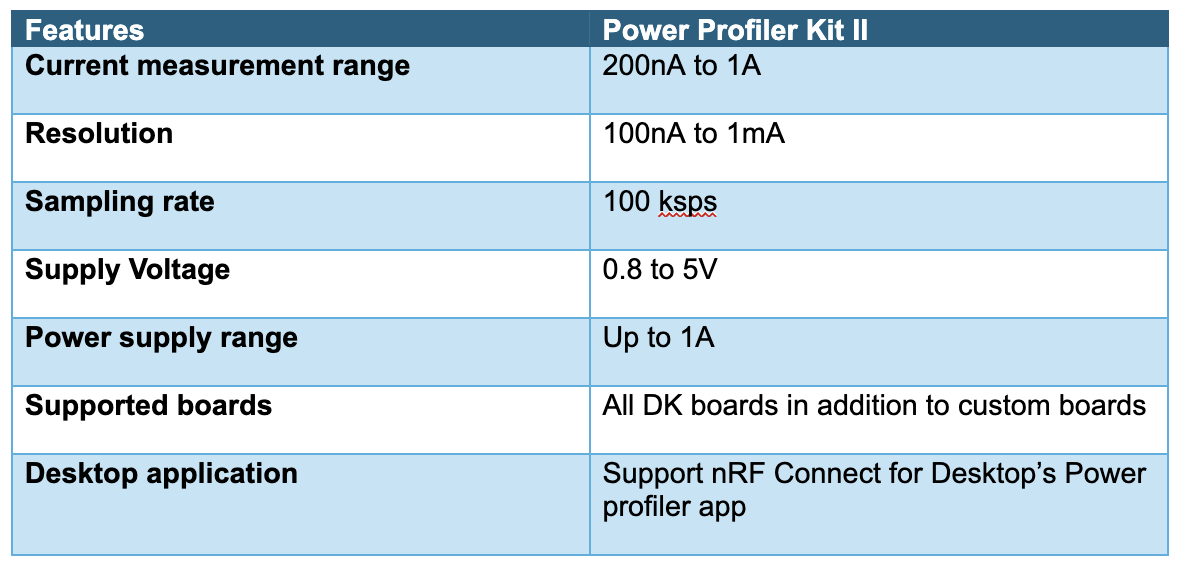
\includegraphics[width=0.6\textwidth]{Materials/figure5}
    \label{materials_5}
    \caption{Power Profiler Kit table}
\end{figure}


\section{Memory management}

The memory architecture of the Nordic board is intricately designed to optimize performance and flexibility. The system comprises various memory regions and buses interconnected to facilitate efficient data transfer and processing. Below is a detailed explanation of each component that resulted from studying nordic documentation \cite{NordicSemiconductorInfocenter}:

Central Processing Unit (CPU) ARM Cortex-M4: The CPU is based on the ARM Cortex-M4 architecture, which is a highly efficient processor designed for high-performance, low-power applications. It includes a rich set of features such as floating-point unit (FPU), digital signal processing (DSP) extensions, and low-latency interrupt handling.
2. Memory Organization
The memory is divided into several sections, each serving a specific purpose and connected via different buses to optimize performance.

RAM Sections (AHB Slaves)
The system contains multiple RAM sections, each interfaced through the Advanced High-performance Bus (AHB). These sections are labeled from RAM0 to RAM8, with each section further divided into smaller subsections. The sections are organized as follows:

RAM0 to RAM8: These RAM sections are accessible via the System bus, DCODE, and ICODE buses, providing flexible access paths for different types of data operations. Each RAM section is split into two subsections (Section 0 and Section 1), and their memory addresses are specified for both data RAM (System) and code RAM (ICODE/DCODE).

Memory Addresses: The RAM sections have designated address ranges:

Data RAM (System): with range \textbf{0x2000\_0000 - 0x2003\_8000}.
Code RAM (ICODE/DCODE): Corresponding code addresses range \textbf{0x0080\_0000 - 0x0083\_8000}.
Flash Memory
Flash memory is used for non-volatile storage, providing persistent data retention even when the system is powered down. The flash memory is divided into pages and accessed via the ICODE and DCODE buses.
Flash Pages: The flash memory is organized into pages, with the address range for flash starting at \textbf{0x0000\_0000} and extending to \textbf{0x000F\_F000}.
Page Addresses: Specific addresses for pages include:
Page 0: \textbf{0x0000\_0000}
Page 1: \textbf{0x0000\_1000}
Page 2: \textbf{0x0000\_2000}
Subsequent pages follow this addressing pattern up to Page 255.
3. Bus Architecture
The system utilizes a multilayer AHB interconnect to manage data flow between different components efficiently.

Advanced High-performance Bus (AHB)
The AHB multilayer interconnect ensures high-speed data transfer between the CPU, RAM sections, flash memory, and peripherals. It allows multiple masters (such as the CPU and DMA controllers) to access shared resources without significant performance bottlenecks.

The Non-Volatile Memory Controller (NVMC) handles writing and erasing tasks for internal flash memory and UICR, requiring specific conditions such as word-aligned addresses and halted CPU during operations. The flash memory is divided into pages, with restrictions on rewriting bits and a limitation on the number of writes before a page erase is necessary.

The NVMC includes an instruction cache (I-Cache) for the ICODE bus, which significantly enhances CPU performance by reducing flash memory access times. A cache hit retrieves instructions from the cache with no delay, while a cache miss incurs a delay as the instruction is fetched from flash. This setup can lower power consumption, depending on the cache hit rate. Profiling tools within the NVMC allow for the analysis of cache efficiency, tracking hits and misses to optimize performance.

Partial page erases are also supported to minimize CPU stalls in critical operations by dividing erase operations into shorter chunks, especially useful in time-sensitive applications. This feature does not apply to UICR.

System Bus, DCODE, and ICODE
These buses provide specific pathways for different types of data access:

System Bus: Used for general data transfers.
DCODE Bus: Dedicated to instruction fetches from flash memory.
ICODE Bus: Used for instruction fetches from both RAM and flash memory, enabling efficient code execution.
4. Peripherals and EasyDMA
Peripherals: The system includes various peripherals connected via the AHB2APB bridge, allowing integration with different peripheral devices.
EasyDMA: Direct Memory Access (DMA) controllers facilitate direct data transfers between peripherals and memory, bypassing the CPU to enhance efficiency. EasyDMA controllers are connected via DMA buses to the peripheral modules.
5. Address Mapping
The memory map clearly defines the address ranges for each memory section and peripheral, ensuring well-organized access to system resources.
RAM Sections: Each RAM section has a specific address range, both for system data and code execution, ensuring organized and conflict-free memory access.
6. Interconnect and Bus Matrix
The AHB multilayer interconnect/bus matrix allows concurrent access to different memory sections and peripherals, reducing latency and improving overall system throughput.

The Nordic board's memory architecture is a sophisticated system designed for efficient data handling and high performance. By leveraging multiple RAM sections, a well-organized flash memory layout, and an advanced bus interconnect system, the architecture supports the demanding requirements of modern embedded applications. The integration of DMA controllers further enhances data transfer efficiency, making the Nordic board suitable for a wide range of applications requiring reliable and high-speed memory access.

\subsection{Overview of the Address Map}
The memory architecture of the Nordic board is intricately designed to optimize performance and flexibility. The system comprises various memory regions and buses interconnected to facilitate efficient data transfer and processing.
The address map is divided into two main sections: the System Address Map and the Address Map for peripherals. The System Address Map shows the hierarchical arrangement of different memory regions and device spaces, while the Address Map specifies the address ranges for peripherals and other key components.

\subsection{System Address Map}

\textbf{Device Space (0xE0000000 - 0xFFFFFFFF)}
This region is reserved for device-specific addresses, typically used for system control and private peripheral bus (PPB) mappings. The PPB includes critical control registers for system-level operations such as interrupts and debugging.

\textbf{RAM (0x80000000 - 0xBFFFFFFF)}
This region is designated for RAM, divided into two main blocks:
\begin{itemize}
    \item \textbf{0x80000000 - 0x9FFFFFFF}: General RAM space.
    \item \textbf{0xA0000000 - 0xBFFFFFFF}: Additional RAM or special-purpose RAM.
\end{itemize}

\textbf{Peripheral Space (0x60000000 - 0x7FFFFFFF)}
This area is allocated for peripheral devices, allowing the CPU to interact with various hardware modules via memory-mapped I/O.

\textbf{SRAM (0x40000000 - 0x5FFFFFFF)}
This region is dedicated to SRAM, providing fast, volatile memory storage for critical data that requires quick access times.

\textbf{Code Space (0x00000000 - 0x1FFFFFFF)}
This segment includes different types of memory used for storing executable code:
\begin{itemize}
    \item \textbf{0x00000000 - 0x007FFFFF}: Flash memory for non-volatile code storage.
    \item \textbf{0x00800000 - 0x00FFFFFF}: Code RAM for executing code from RAM.
    \item \textbf{0x10000000 - 0x10000FFF}: FICR (Factory Information Configuration Registers) containing device-specific configuration data.
    \item \textbf{0x12000000 - 0x12000FFF}: UICR (User Information Configuration Registers) for user-specific configuration.
    \item \textbf{0x19FFFFFF - 0x20000000}: XIP (Execute In Place) memory, allowing execution directly from external flash.
\end{itemize}

\subsection{Peripheral Address Map}

\textbf{Private Peripheral Bus (0xE0000000)}
The PPB includes system control space (SCS), NVIC (Nested Vectored Interrupt Controller), and other essential control registers.

\textbf{AHB Peripherals (0x50000000)}
This range is used for high-performance peripherals connected via the Advanced High-performance Bus (AHB), providing efficient data transfer capabilities.

\textbf{APB Peripherals (0x40000000)}
The Advanced Peripheral Bus (APB) space is designated for slower peripherals that do not require the high throughput provided by the AHB.

\subsection{Detailed Address Ranges and Usage}

\textbf{Flash Memory (0x00000000 - 0x007FFFFF)}
Used for storing the firmware and application code. Flash memory is non-volatile, retaining data even when power is off.

\textbf{Code RAM (0x00800000 - 0x00FFFFFF)}
Provides a space for loading and executing code from RAM, useful for applications requiring high-speed code execution.

\textbf{FICR (0x10000000 - 0x10000FFF)}
Contains factory-programmed data specific to the device, such as calibration values and unique identifiers.

\textbf{UICR (0x12000000 - 0x12000FFF)}
Stores user-programmable configuration data, which can include bootloader settings and memory protection configurations.

\textbf{XIP (0x19FFFFFF - 0x20000000)}
Allows the system to execute code directly from external flash memory, saving internal RAM for other uses.

\subsection{Summary}
The Nordic board's memory architecture is designed to efficiently manage various types of memory and peripheral access. The system address map and peripheral address map clearly define regions for devices, RAM, peripherals, and code execution. This structured organization allows for optimized performance, flexibility in code execution, and efficient interaction with peripherals.

By understanding this memory layout, we, as developers, can make informed decisions about memory usage, peripheral integration, and system optimization, ultimately enhancing the performance and functionality of applications running on the Nordic board.

Based on the detailed analysis of the Nordic board's memory architecture, several key observations can be made to optimize code and effectively manage memory. These recommendations will help enhance the performance and efficiency of their applications.

\subsection{Utilizing Flash Memory for Code Storage}
\textbf{Observation:}
\begin{itemize}
    \item Flash memory (0x00000000 - 0x007FFFFF) is non-volatile and ideal for storing the firmware and application code.
\end{itemize}

\textbf{Recommendation:}
\begin{itemize}
    \item Store all static code and infrequently updated data in flash memory to ensure data persistence across reboots and power cycles.
    \item Optimize the code to minimize the frequency of flash writes, as flash memory has a limited number of write cycles.
\end{itemize}

\subsection{Efficient Use of Code RAM}
\textbf{Observation:}
\begin{itemize}
    \item Code RAM (0x00800000 - 0x00FFFFFF) allows for high-speed code execution.
\end{itemize}

\textbf{Recommendation:}
\begin{itemize}
    \item Load performance-critical code segments and frequently accessed functions into Code RAM to benefit from faster execution times.
    \item Use this space judiciously due to its limited size, prioritizing code that requires low-latency access.
\end{itemize}

\subsection{Managing Volatile Data with SRAM}
\textbf{Observation:}
\begin{itemize}
    \item SRAM (0x40000000 - 0x5FFFFFFF) provides fast, volatile memory for temporary data storage.
\end{itemize}

\textbf{Recommendation:}
\begin{itemize}
    \item Use SRAM for variables, stack, and heap allocation that require quick read/write access.
    \item Regularly monitor SRAM usage to prevent stack overflows and ensure efficient memory allocation.
\end{itemize}

\subsection{Leveraging XIP for External Code Execution}
\textbf{Observation:}
\begin{itemize}
    \item XIP (0x19FFFFFF - 0x20000000) enables execution directly from external flash memory.
\end{itemize}

\textbf{Recommendation:}
\begin{itemize}
    \item Utilize XIP for large codebases or rarely executed code to free up internal RAM and Flash memory.
    \item Ensure that the execution speed from external memory meets the application's performance requirements.
\end{itemize}

\subsection{Using FICR and UICR for Configuration Data}
\textbf{Observation:}
\begin{itemize}
    \item FICR (0x10000000 - 0x10000FFF) and UICR (0x12000000 - 0x12000FFF) store factory and user-specific configuration data, respectively.
\end{itemize}

\textbf{Recommendation:}
\begin{itemize}
    \item Store device-specific and user-defined configuration settings in FICR and UICR.
    \item Use these regions to keep calibration data, unique identifiers, and bootloader settings.
    \item These registers should be written infrequently to avoid wear.
\end{itemize}

\subsection{Optimizing Peripheral Access}
\textbf{Observation:}
\begin{itemize}
    \item AHB (0x50000000) and APB (0x40000000) peripheral spaces are designated for high and low throughput peripherals.
\end{itemize}

\textbf{Recommendation:}
\begin{itemize}
    \item Map high-speed peripherals that require frequent access to the AHB space for efficient data transfers.
    \item Use the APB space for peripherals with lower bandwidth requirements.
    \item Ensure that peripheral access patterns do not create bottlenecks, particularly in real-time applications.
\end{itemize}

\subsection{Balancing RAM and Peripheral Usage}
\textbf{Observation:}
\begin{itemize}
    \item The board has multiple RAM sections and peripheral regions connected via AHB and APB buses.
\end{itemize}

\textbf{Recommendation:}
\begin{itemize}
    \item Distribute memory usage across different RAM sections to avoid contention and ensure balanced load.
    \item Efficiently manage DMA transfers to minimize CPU involvement in data movement between peripherals and memory, thus improving overall system performance.
\end{itemize}

\begin{figure}[H]
    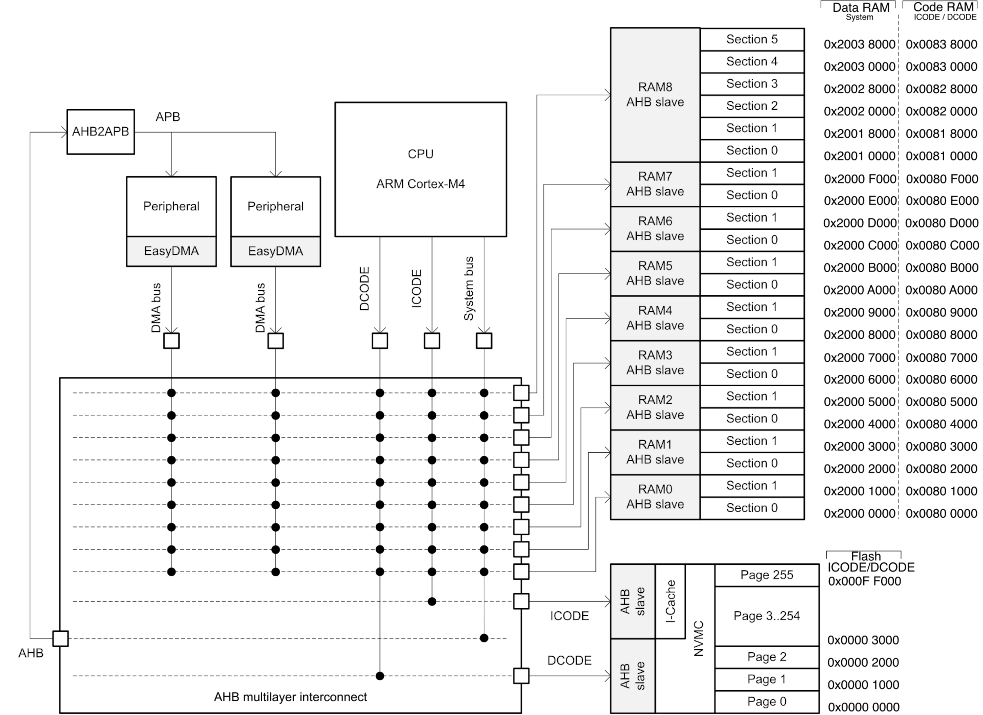
\includegraphics[scale=0.3]{memNRF.png}
    \centering
    \label{mem_table_1}
    \caption{Memory table for the board \cite{NordicSemiconductorInfocenter}}
    \end{figure}

\begin{figure}[H]
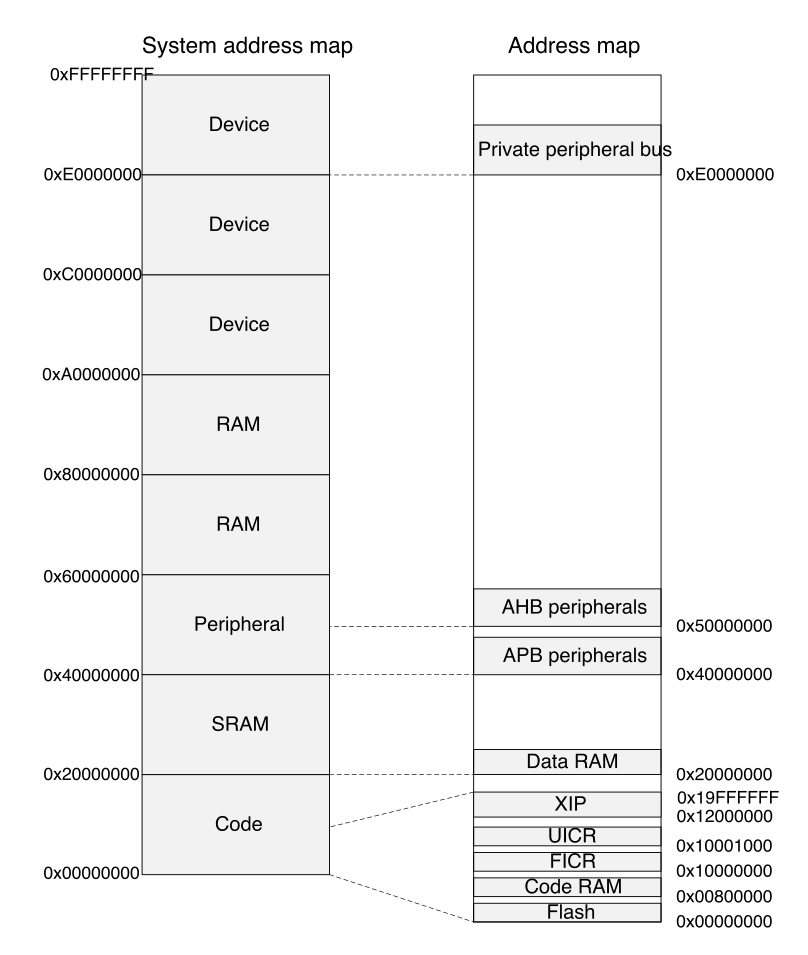
\includegraphics[scale=0.4]{memory2.png}
\centering
\label{mem_table_2}
\caption{Memory table for the board \cite{NordicSemiconductorInfocenter}}
\end{figure}

\section{Channel selection}

We have already described in previous sections the project at hand and why every possible improvement can ease the development of a functional implementation.
One of those crucial aspects is the amount of information sent between the devices, in the particular the channels that get transmitted.
As previously shown, the dataset at hand was registered using cuff electrodes chirurgically implanted on the animals' peripheral nerves; each of these cuff electrodes has 16 sensors that are able to measure the voltage of the nerve they cover.
Each of these sensors, being in a different position, will register different data, furthermore one or more of these sensors may be damaged during the surgery or may record data with high noise.
Because of this, not only it would be useful to limit the channel we share between devices to help with the communication, but we could also help the classifier by removing channels with faulty or noisy sensors.
In short, the three benefits of channel selection are : reducing the computational complexity of any process on the dataset, reduce the amount of overfitting of the models and reudce the times to setup the application. \cite{alotaibyReviewChannelSelection2015}
There is a great amount of literature that deals with the issues of channel selection of EEG channels, since it is a well known area of research and proves to be very helpful in reaching better results.
In particular our area of interest focused on channel selection applied to motion-imagery EEG Signals (MI-EEG).
We will now present an overview of the most relevant methods for channel selection.

\subsection{Common spatial patterns methods}

Common Spatial Patterns (CSP) is a popular algorithm used in neuroscience, particularly in brain-computer interfaces (BCI), to enhance feature extraction from multichannel signals, such as EEG (electroencephalography) data. CSP is especially useful for distinguishing between two classes of motor imagery or other cognitive tasks by identifying spatial filters that maximize the variance for one class while minimizing it for the other.
Common spatial patterns (CSP) method was firstly suggested for classification of multi-channel EEG during imagined hand movements by H. Ramoser \cite{ramoserOptimalSpatialFiltering2000}. The core concept involves employing a linear transformation to map multi-channel EEG data into a reduced-dimensional spatial realm using a projection matrix. Each row of this matrix represents channel weights. This process aims to optimize the variance of signal matrices for two classes. The CSP method relies on concurrently diagonalizing the covariance matrices of both classes. \cite{abdullahEEGChannelSelection2022}

Let X $\epsilon$ $R^{M x N}$ denote a matrix of EEG, where the channel number is M and the samples are denoted by N. The classic CSP problem is stated as follows:

\begin{align}
	\max_{W \epsilon R^{M}} = \frac{W^{T} C_1 W}{W^{T} C_2 W}
	\label{eq:CSP1}
\end{align}

where W is a spatial filter coefficient, $C_{i}$(i=1,2) indicates a single-class covariance matrix. The generalised eigenvalue decomposition (EVD) generally can handle this problem. \cite{abdullahEEGChannelSelection2022}

\subsubsection{Sparse CSP}

Due to classic CSP inadequacies, several researchers aim to integrate sparsing behavior with conventional CSP to discover and eliminate highly noisy or interfering channels. Given w’s sparsity k, i.e., the number of nonzero items in w. The sparse CSP problem is stated as follows:

\subsubsection{Regularized CSP}

Despite its well-established efficacy and widespread adoption, CSP is acknowledged for its susceptibility to noise and tendency for overfitting. To tackle this concern, researchers have proposed the regularization of CSP \cite{lotteRegularizingCommonSpatial2011}. A recommended strategy is the adoption of a regularized CSP (RCSP) approach, which focuses on regulating the covariance matrix estimate within CSP extraction. This involves employing regularization techniques derived from general learning principles \cite{friedmanRegularizedDiscriminantAnalysis1989,wangSolvingFaceRecognition2006}. The regularization of CSP can occur at two levels, the first being at the estimation of the covariance matrix. Since CSP relies on these estimates, which can be adversely affected by noise or limited training data, regularization can significantly improve performance. Alternatively, regularization can be implemented at the objective function level, where spatial filters are subjected to prior constraints to enhance stability \cite{lotteRegularizingCommonSpatial2011}.

The first, based on \cite{luRegularizedCommonSpatial2009} can be implemented in the following way:

\begin{align}
	\tilde{C}_{C} = (1 - \gamma) \hat{C}_{C} + \gamma I
	\label{eq:RCSP1}
\end{align}

\begin{align}
	\hat{C}_{C} = (1 - \beta) {s}_{C} {C}_{C} + \beta {G}_{C}
	\label{eq:RCSP2}
\end{align}


where $C_{c}$ is the initial spatial covariance matrix for class $c$, $\tilde{C}_{c}$ is the regularized estimate, $I$ is the identity matrix, $S_{c}$ is a constant scaling parameter (a scalar), $\gamma$ and $\beta$ are the two user-defined regularization parameters ($\gamma$, $\beta \in [0,1]$), and $G_{c}$ is a “generic” covariance matrix. \cite{lotteRegularizingCommonSpatial2011}

Another approach to obtain RCSP algorithms consists in regularizing the CSP objective function itself (1). More precisely, such a method consists in adding a regularization term to the CSP objective function in order to penalize solutions (i.e., resulting spatial filters) that do not satisfy a given prior. Formally, the objective function becomes:

\begin{align}
	{J}_{P_{1}}(w) = \frac{w^{T}C_{1}w}{w^{T}C_{2}w + \alpha P(w)}
	\label{eq:RCSP3}
\end{align}

where P(w) is a penalty function, measuring how much the spatial filter w satisfies a given prior. The more w satisfies it, the lower P(w). Hence, to maximize JP1(w), we must minimize P(w), thus ensuring spatial filters satisfying the prior. $\alpha$ is a user-defined regularization parameter ( $\alpha$ $\geq$  0, the higher $\alpha$, the more satisfied the prior). With this regularization, we expect that enforcing specific solutions, due to priors, will guide the optimization process toward good spatial filters, especially with limited or noisy training data. \cite{lotteRegularizingCommonSpatial2011}

% ciao \ref*{cap}

\subsection{Correlation-based methods}

These methods help identifying which subsets of channels is the most relevant by defining a correlation metric and ranking higher those channels that show stronger similarities between them according to the metric.
There are various ways in which we can score the correlation between signals of different channels and here we will briefly present three.

\subsubsection{Spectral entropy dunno first citation}

Spectral entropy is a generic measure of disorganization of signal, as expressed in \cite{yangEEGChannelSelection2018b} with the following formulas:

\begin{align}
H(E)=-\sum_{i=1}^N p\left(E_i\right) \log _{10} p\left(E_i\right),
\end{align}

where \( \mathcal{E} = \{ \mathcal{E}_1, \mathcal{E}_2, \ldots, \mathcal{E}_n \} \) is the signal in the time domain. \( p(\mathcal{E}_i) \) is the probability of \( \mathcal{E}_i \). It is usually estimated by Burg's algorithm. \cite{schalkBCI2000GeneralpurposeBraincomputer2004} \\
Spectral entropy separates the background noise from the organized signal, the motor imagery in this study.

The 'interested class versus the rest' strategy is adopted for the channel selection using the correlation coefficient method. EEG data are split into two groups, \( s_1 \) and \( s_2 \), where \( s_1 \) is the group containing the class of interest. \\
Spectral entropy \( H_1 \) and \( H_2 \) are identified corresponding to \( s_1 \) and \( s_2 \). Correlation of the spectral entropy from the two groups, \( s_1 \) and \( s_2 \), is an indicator of how closely these two groups have a linear relationship, written as:

\begin{align}
\rho\left(H_{1, j}, H_{2, j}\right)=\frac{\operatorname{cov}\left(H_{1, j}, H_{2, j}\right)}{\sigma_{H_1, j} \sigma_{H_2, j}},
\end{align}

where \( \sigma_{H_j} \) is the standard deviation of the respective spectral entropy. \( j \) is the index of the channel. \\
 For the purpose of channel selection, we consider the spectral entropy of each channel across all frequency ranges by taking the sum of the squared correlation coefficient,

\begin{align}
P\left(H_{1, j}, H_{2, j}\right)=\sum_{i=1}^N \rho^2\left(H_{1, j}, H_{2, j}\right),
\end{align}

where $i$ = 1 - $N$ is the number of frequency bins during estimation of the spectral entropy.

\subsubsection{Pearson’s Correlation Coefficient }

Pearson correlation coefficient is a statistical association or linear dependence between two or more random variables and, in our case, it can measure the linear correlation between two channels. \cite{thibeaultUsingHybridNeuron2013}


\begin{align}
	\rho (X,Y) = \frac{1}{n-1} \sum_{i}^{N}(\frac{X_i - \bar{X}}{\sigma_{X}})( \frac{Y_i - \bar{Y}}{\sigma_{Y}})
	\label{eq:correlationCoefficient}
\end{align}

Considering the two variables, denoted as \( X \) and \( Y \), with \( n \) representing the number of observations, \( \bar{X} \) and \( \bar{Y} \) as their respective means, and \( \sigma_X \) and \( \sigma_Y \) as the default deviations between them, the correlation coefficient \( \rho(X,Y) \) ranges from 0 to 1. This range indicates the strength of the relationship, varying from low to high. In this context, the correlation coefficient is computed for each pair of EEG channels.

\subsubsection{Cross-Correlation Based Discriminant Criterion (XCDC)}
XCDC is a correlation method used to evaluate the informativeness of a channel for classification tasks by measuring its similarity to other channels. It calculates the cross-correlation between two EEG signals after z-score normalization to account for amplitude effects. The method then defines within-class similarity and between-class dissimilarity, which are combined into a discriminant score D. Channels are ranked based on this score, with higher scores indicating more informative channels. The score D is determined by a weighted combination of within-class and between-class measures, tuned via a hyperparameter $\lambda$.

We will discuss it more in depth in Chapter $4$, since this is the algorithm we chose for our channel selection.

Here is a less precise overview of the algorithm's formulas.
With S defined as the scoring function for the correlation between the signals.

\begin{align}
	S(x,y) = \max(r_{x\hat{y}(k)}), k=0,1,..., T - 1 
   \label{eq:XCDC_01}
\end{align}

Same class score defined as:
\begin{align}
	R_w = \mathbf{mean}(S(\tilde{x_i}\tilde{x_j}| c_i = c_j))
   \label{eq:XCDC4}
\end{align}

Different class score defined as:
\begin{align}
	R_b = -\mathbf{mean}(S(\tilde{x_i}\tilde{x_j}| c_i \neq  c_j))
   \label{eq:XCDC5}
\end{align}
where $c_i$ is the class label of the i-th trial.

The discriminant score D is then defined as follows:
\begin{align}
	D = \lambda R_w + (1-\lambda)R_b
   \label{eq:XCDC6_1}
\end{align}

in which $\lambda$ is a weighting hyperparameter to be tuned empirically.
Channels are ranked in a descending order according to their discriminant score D after obtaining D for every channel using.


\subsection{Sequential Based methods}

These methods implement a sequential approach where top features are identified iteratively.
The most common example of Sequential method is the Sequential Forward Selection that was first used for variable selection by Whitney (1971). \\
It begins the research with an empty set of features, all the features are evaluated according to their impact on the evaluation metric and then, the variable with the best effect gets added to the subset of features. \\
This step gets re-iterated untill all the variables are progressively included in the set for comparisons purposes.
SFS has what is defined as the "nesting property" which means that once a feature gets included in the subset, that feature stays in the subset even if removing it would improve the results.  \cite{reunanenOverfittingMakingComparisons}
A different version is the Sequential Backward Search which functions identically but starts from a full set of variables and removes one them one by one according to the worst impact on the evaluation metrics. \cite{pudilFloatingSearchMethods1994} \\
Both of these methods' complexity is O($n^2$). \cite{kudoComparisonAlgorithmsThat2000}

\subsubsection{Sequential Floating Forward Selection (SFFS)}

The sequential forward floating selection has in many instances demonstrated to be a superior algorithm.\cite{reunanenOverfittingMakingComparisons} \cite{zongkerAlgorithmsFeatureSelection1996}
In our case in particular by addressing the nesting issue we better account for two features that highly impact the evaluation metrics but being highly correlated effectively carry the same information and may be not be both relevant to the final subset of features.
It returns a better subset of feature at the cost of a higher complexity of O($2^n$). \cite{kudoComparisonAlgorithmsThat2000} \\
The core approach utilized in Sequential Floating Forward Selection (SFFS) to address nesting issues involves initiating a backtracking phase after the addition of each variable. During this phase, variables are systematically excluded until superior subsets of corresponding sizes are identified. This process continues until no better subset is discovered, prompting a return to the initial step to include the best previously excluded variable. Subsequently, another backtracking phase ensues. \cite{reunanenOverfittingMakingComparisons} \cite{ pudilFloatingSearchMethods1994} \\ 
In the original work of Pudil (1994) it is also proposed a floating version of the SBS called SBFS that implements the same idea but once again starting with a full set of features and removing them iteratively. Its complexity is O($2^n$).

\subsubsection{Generalized Sequential Forward Selection (GSFS) }

Generalized Sequential Forward Selection (GSFS) is an extension of the Sequential Forward Selection (SFS) algorithm. \\
In GSFS, similar to SFS, the algorithm starts with an empty set of features and iteratively adds features to the model based on some evaluation criterion, such as minimizing error or maximizing predictive performance. However, GSFS introduces additional flexibility by allowing the inclusion of multiple features at each step instead of just one. This can potentially speed up the feature selection process and lead to better performance by considering feature combinations more efficiently.

The key idea behind GSFS is to explore feature subsets in a more generalized manner, considering not only individual features but also combinations of features at each step of the selection process. This can be particularly useful in situations where interactions between features are important for modeling complex relationships in the data.

Overall, GSFS offers a more flexible and comprehensive approach to feature selection compared to traditional forward selection methods like SFS, making it suitable for a wide range of applications in machine learning and data analysis. \cite{radmanGeneralizedSequentialForward2019}
GSFS and the backward implementation GSBS, both have a complexity that depend of the number of features they can add per iteration, if we define g as the number of features added per iteration, then their complexity is O($n^{g+1}$). \\
 With g = 1 GSFS is equal to SFS.

\subsection{Binary Particle Swarm Optimization Based methods}

In 1995, the PSO algorithm was presented by Kennedy and Eberhart. \cite{okwuMetaheuristicOptimizationNatureInspired2020} \\
Binary Particle Swarm Optimization (BPSO) is an adaptation of the traditional Particle Swarm Optimization (PSO) algorithm designed to work with discrete, binary search spaces. It is commonly used in feature selection and optimization problems where solutions are represented by binary variables (0 or 1).
The idea behind it is inspired by the social behavior of birds flocking or fish schooling. \cite{vanneschiParticleSwarmOptimization2023}
In standard PSO, particles move around in a continuous solution space, adjusting their positions and velocities based on their own best-known position and the global best-known position found by any particle in the swarm.
\\
This collective learning process guides the particles toward better regions of the search space, converging to the optimal solution. \\
The balance between exploration (searching for new solutions) and exploitation (refining known solutions) is controlled by various parameters such as inertia weight, cognitive factor, and social factor. \\
Example update functions for position ($x_{i}(t+1)$) and speed ($v^{i}_{k+1}$) are as follows from Abdullah\cite{abdullahEEGChannelSelection2022}:

\begin{align}
	v_{k+1}^i=w v_k^i+c_1 r_1\left(p_k^i+x_k^i\right)+c_2 r_2\left(g b e s t-x_k^i\right)
	\label{eq:bpso1}
\end{align}
\begin{align}
	x_i(t+1)=x_i t+v_i(t+1)
	\label{eq:bpso2}
\end{align}

where i represents the i-th particle. $c_1$ is the cognitive coefficient and $c_2$ is the social one. They regulate how fast the particle is going and are both constant. $w$ is the inertial weight which limits the speed. $r_1$,$r_2$ are random values between 0 and 1. $k$ represents the iteration of the update function. $t$ represents the time. $p^{i}_{k}$ represents the best solution found so far by the i-th particle at k-th iteration. gbest is the best position found by the swarm so far.
Just below we present a visualization of particle movement in a 3D space. 

\begin{figure}[H]
	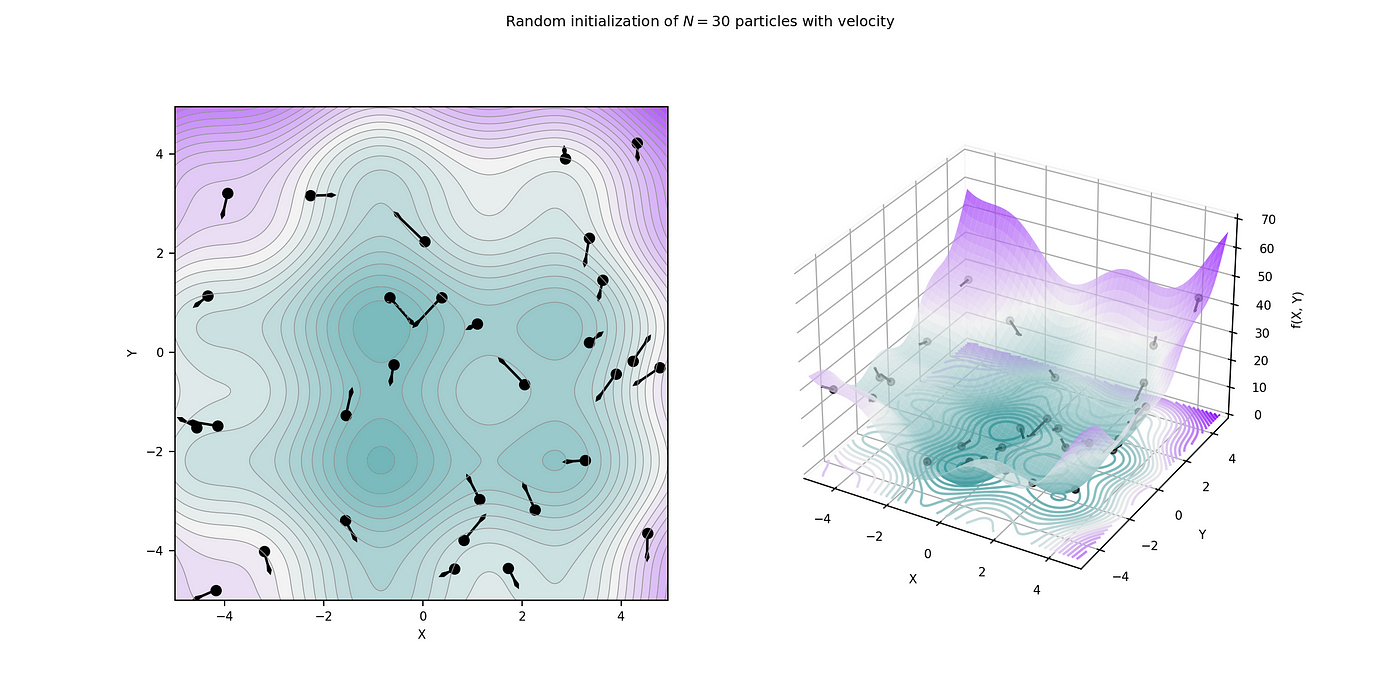
\includegraphics[scale=0.35]{pso.png}
    \label{pso}
	\caption{Illustration of particles moving in a 3D space}
\end{figure}

PSO has also a binary implementation called Binary Particle Swarm Optimization (BPSO).
The basic principles of BPSO are similar to those of standard PSO, with particles searching for the optimal solution through iterative updates of their positions and velocities. However, in BPSO, the binary representation of the particle's position is manipulated using binary operators such as bitwise AND, OR, and NOT, instead of arithmetic operations used in continuous PSO. \cite{kennedyDiscreteBinaryVersion1997}

The binary version suits feature selection since the binary values represent whether a feature is present or not in the subest of the most relvevant features.

We present here the updated equations for BPSO, the main difference being that here the position of the particle can either be 1 or 0. \cite{abdullahEEGChannelSelection2022}


\begin{align}
S(v) &= \left(1+e^{-v}\right)^{-1} \\
x_{k+1}^i &=1 \:\:\:\:\:\: \text { if } \tau<S\left(v_{k+1}^i\right) \\
x_{k+1}^i &=0 \:\:\:\:\:\: \text { if } \tau>S\left(v_{k+1}^i\right),
\end{align}

With v defined as previously in PSO, and S being a logistic function that varies from 0 to 1.
We decide if the position of the i-th particle is 1 or 0 depending on the $\tau$.
There are also multi-objective versions for both PSO and BPSO called Multi-Objective Particle Swarm Optimization (MOPSO) and Binary Multi-Objective Particle Swarm Optimization respectively (BMOPSO). \cite{coellocoelloMOPSOProposalMultiple2002}


% \subsubsection{Other method: Fisher's criterion}

% The aim of channel selection is to select the most discriminative EEG channels from the original 30 channels by applying the Fisher's criterion. The FD features from the 30 channels are concatenated to a feature vector (called data hereafter) of dimension q
% , where q=30
% . Let 𝐱𝑖𝑗∈𝑅𝑞
%  denotes the jth training data of class 𝑖
% , where 𝑖=1,…, 𝑐
% , 𝐦𝑖
%  is the mean of the training data of the ith class, and 𝐦
%  is the mean of the training data from all classes. In this study, we focused on the classification problem in a motor imagery task (resting vs. motor imagery). Thus, 𝑐=2
% . The within-class 𝐒𝑤
%  and the between-class 𝐒𝑏
%  scatter matrices are calculated by

%  \cite{liuMotorImageryEEG2017}

 
% \begin{aligned}
% & \mathbf{S}_w=\sum_{i=1}^c P_i\left(\frac{1}{n_i} \sum_{j=1}^{n_i}\left(\mathbf{x}_{i j}-\mathbf{m}_i\right)\left(\mathbf{x}_{i j}-\mathbf{m}_i\right)^t\right) \\
% & \mathbf{S}_w=\sum_{i=1}^c P_i\left(\frac{1}{n_i} \sum_{j=1}^{n_i}\left(\mathbf{x}_{i j}-\mathbf{m}_i\right)\left(\mathbf{x}_{i j}-\mathbf{m}_i\right)^t\right)
% \end{aligned}

% respectively, where 𝑛𝑖
%  denotes the number of data in the ith class, the superscript ‘t’ stands for the transpose of a matrix, and 𝑃𝑖=𝑛𝑖/∑𝑐𝑗=1𝑛𝑗
%  is the prior probability of the ith class. The class separability for the fth feature (𝑓=1,…,𝑞
% ) can be represented by the Fisher score 𝐹(𝑓)
% As

% \begin{aligned}
% F(f)=\frac{\mathbf{S}_b(f)}{\mathbf{S}_w(f)}, \quad f=1,2, \ldots, q
% \end{aligned}

% where 𝐒𝑏(𝑓)
%  and 𝐒𝑤(𝑓)
%  are the fth diagonal elements of 𝐒𝑏
%  and 𝐒𝑤
% , respectively. The higher the value of 𝐹(𝑓)
%  is, the better the class separability of the feature extracted from the fth channel is. Based on the class separability criterion, we can select 𝑑
%  top channels among the 30 ones. The 𝑑
%  features from the selected channels are concatenated to a feature vector.

\subsubsection{Dataset and results}


We sought to identify an algorithm that not only excelled in standard performance metrics like Accuracy and F1 Score while minimizing the number of channels but also integrated seamlessly with our existing models. Given the architecture of our ENGNet model, it was crucial to find a channel selection algorithm that could operate effectively within a Neural Network framework.
Moreover, considering future test scenarios, we required an algorithm capable of functioning in an "online" manner, or as close to real-time processing as possible. This need arose because of the potential application of our model in environments where rapid processing and adaptability are critical.

\textbf{Requirements Summary}
\begin{itemize}
    \item Online or near-online operation
    \item Compatibility with CNN-based models
    \item Strong performance in F1 Score and Accuracy
    \item Effective with a reduced number of channels
\end{itemize}

While many algorithms focus on noise reduction, these approaches are already integrated within ENGNet through spatial feature extraction. This was also why Adaptive Signal Reconstruction (ASR) did not show significant improvement; the spatial filtering capabilities already present in ENGNet addressed similar challenges.


Ideally, we would have liked to perform channel selection by iterating over all possible subsets of features; however, this approach is computationally prohibitive due to the time required. Similarly, methods like Particle Swarm Optimization were dismissed for the same reason—they are too time-consuming.

Instead, we turned to correlation-based algorithms, which have shown promise and been tested with CNNs. Since our model already utilizes CNNs, we explored the possibility of implementing a new algorithm that, while not extensively tested, would only require the addition of one layer to our existing structure. The main challenge with this approach is the typical black-box nature of Neural Networks, but we will address these issues in detail in a later section.
In particular, we will explain in detail the models we chose in the next chapter.


\chapter{Materials and Methods}
% \label{ch:conclusions}%
This chapter delves deeper into the materials and methods we used to both write the firmware code for the boards of the PNRelay project and to work on the algorithms for the channel selection.
Given the limitations at hand, the focus of our work was to try and solve a list of different issues that came up during the development of the project.
In particular:

\begin{itemize}
	\item Optimization of firmware communication parameters
	\item Safe transmission via BLE
	\item Channel selection
	\item Calculation of dissipated power
	\item Memory management
	\item Reversible transmission
\end{itemize}

We will divide this chapter into two main parts: one that is related to the firmware and the hardware aspects, one that is related to the channel selection algorithms.
These two parts have been carried on for the majority of our work indipendently and despite the common goal share little to no similarities as far as materials and methods go.

\section{Firmware: Shift}

\subsection{Shift Algorithm}

Even if in previous firmware implementation the data that were exchanged from one board to the other one were directly generated from the peripheral itself, this would not be the case in the actual implementation, in which data would directly come from the ADC, whose samples will contain information which are relative to neural system. This sampling procedure is done at a frequency of 80 kHz. Each sample will then be provided to the peripheral board, which is the one responsible to send them to central device and then to external unit. All of these data which come from the ADC have as a size 10 bits, which is quite uncomfortable to be threated. The microcontroller, in fact, needs to store the samples, but store them into a \texttt{uint8\_t} variable would implicate a waste of information, variables of 16 bits size would instead guarantee a waste of memory. In the previous implementation, the second approach is adopted, as shown below:


\begin{figure}[H]
    \centering
    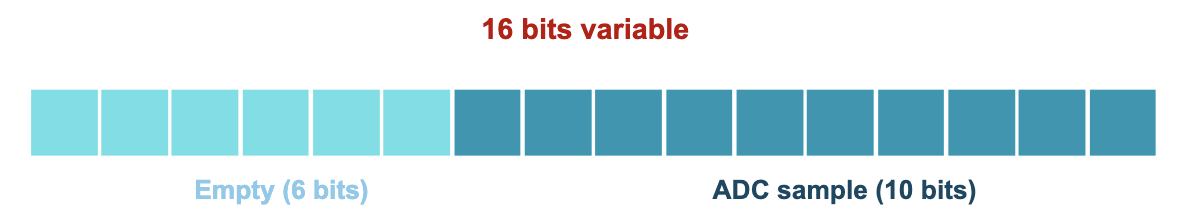
\includegraphics[scale=0.7]{Shift Algorithm/Screenshot 2024-07-22 at 22.31.12.png}
    \caption{Data packing in previous implementation}
    \label{pairing_procedure}
\end{figure}


As mentioned above, this approach is responsible for a great waste of memory. In fact, every time a 10 bits new sample is generated from the ADC, this is saved into 16 bits variables, guaranteeing for each sample a waste of 6 bits. This approach should be improved, because memory in microcontrollers is very limited, and 6 bits out of 16 wasted for each samples means that 6/16 of the throughput obtained is not informative. In all of the online tests two different throughputs are computed as explained below:

\[
\text{Throughput} = \frac{\text{number of bits received from central device}}{\text{elapsed time}}
\]

\[
\text{Real throughput} = \frac{\text{number of bits received from central device} - \text{number of empty bits}}{\text{elapsed time}}
\]

Where the first one represents the effective speed of the BLE communication, while the second one takes into account just the number of bits which contains information, which would result more or less in 10/16 of the first one. In order to have a better understanding of what was happening with previous version of the firmware, the pre-processing operations done for each single BLE packet could be analysed. The function responsible for doing this is the \texttt{Spibuff} function. As previously said, data were generated at a constant frequency of 80 kHz. Once there are enough samples inside the ring buffer to full fill a BLE packet (which means at least 244 bytes), data preprocessing operations were performed. Since each sample has a size which cannot be contained into a single byte, this means 2 bytes are dedicate to each one, and then data preprocessing operation is performed each time 122 samples have been generated from ADC. Once they are, each sample is taken from the ring-buffer. Then, the 8 most informative bits of the \texttt{uint16\_t} variable which temporarily contains it would form the first byte, and the 8 less informative bits would form the second one. This operation is performed 122 times for each BLE packet, in order to full fill them. By making this, the final number of samples reived from central device is a half of the received bytes. The figure below represents this concept in case of an offline test.

\begin{figure}[H]
    \centering
    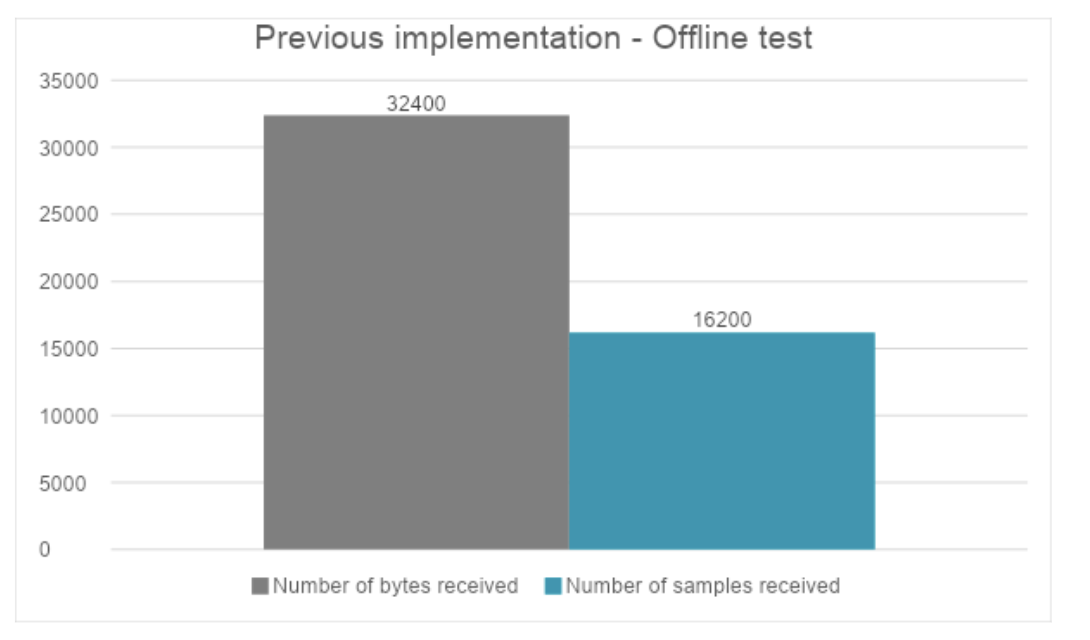
\includegraphics[scale=0.7]{Shift Algorithm/Screenshot 2024-07-22 at 22.31.21.png}
    \caption{Data packing in previous implementation}
    \label{pairing_procedure_2}
\end{figure}

Bytes generation procedure done in previous implementation is schematized below, where the parentheses represent the bytes that would be contained in BLE packet and sent to central device:

\begin{figure}[H]
    \centering
    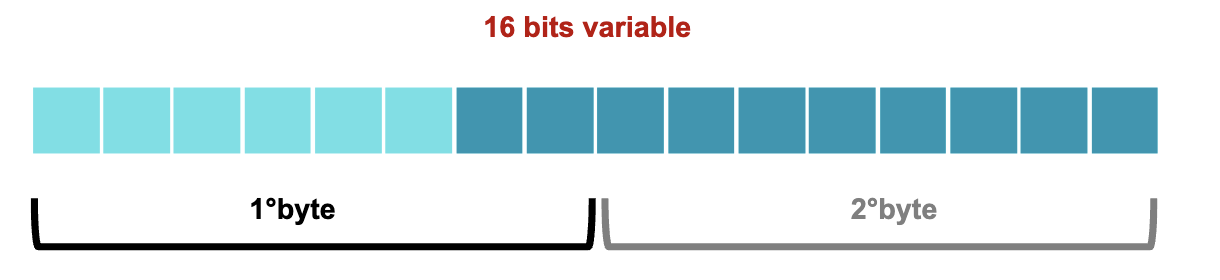
\includegraphics[scale=0.7]{Shift Algorithm/Screenshot 2024-07-22 at 22.31.29.png}
    \caption{Data packing in previous implementation}
    \label{pairing_procedure_3}
\end{figure}


Each couple of bytes would then be packed into the original 16 bits variable in central device, in order to reconstruct the ADC samples. To improve this operation, a shifting algorithm has been implemented. The idea is to perform some bit-masking operations in order to use also those bits which previously were empty. As a consequence, data need to be compressed in the peripheral and then decompressed in central device. A scheme of the compression operation is shown below:

\begin{figure}[H]
    \centering
    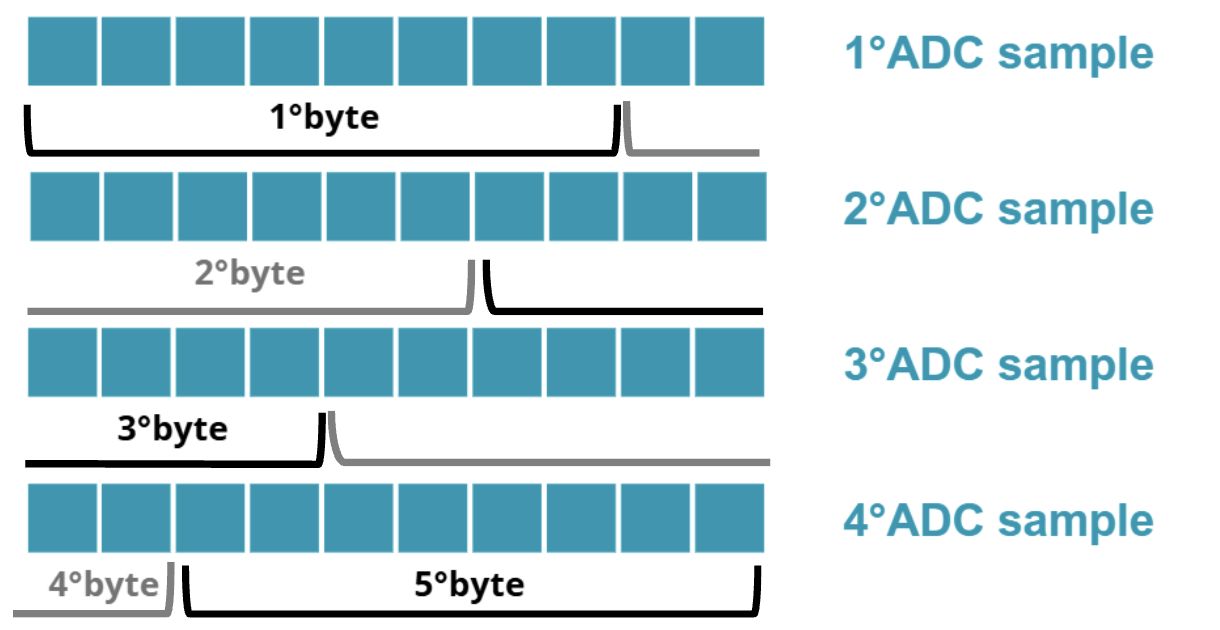
\includegraphics[scale=0.7]{Shift Algorithm/Screenshot 2024-07-22 at 22.31.36.png}
    \caption{Shift algorithm transmitter side}
    \label{pairing_procedure_4}
\end{figure}

To be precise the ADC samples are saved into \texttt{uint16\_t} variables, but since they have a size of 10 bits just the 10 less significant bits out of this 16 are considered. The shifting procedure performed by peripheral can be summarized in the following steps:

\begin{enumerate}
    \item First byte is obtained by taking the 8 most significant bits of the first sample obtained from the ADC.
    \item Second byte is obtained by putting the 2 less significant bits of first sample into the 2 most significant positions and the 6 most significant bits of second sample into the remaining 6 positions.
    \item Third byte is obtained by putting together the four right positioned bits of second sample and the 4 left positioned bits of third sample.
    \item Fourth one is obtained by considering the 6 less significant bits of third sample and the 2 most significant bits of fifth sample.
    \item Lastly, fifth byte is obtained by taking the 8 most rightly positioned bits inside fourth sample.
\end{enumerate}

Once these steps are completed, the procedure becomes periodical, and it is repeated from the beginning. By making this, it can be noted that, in order to send 4 samples, just 5 bytes are necessary and not 8 like in previous implementation. Moreover, each single bit contains information, and it is not wasted. However, it should also be noted that this procedure can only be performed when at least 4 samples have been generated from the ADC, differently from before where just one was necessary. Another limitation is imposed by BLE packet size, which can contain 244 bytes as a maximum value, which is not a number multiple of five. This means that not all of the samples inside a single BLE packet can be shifted if the BLE maximum packet size is maintained.

To be more precise, the generation of a single BLE packet can be analysed as done for the previous implementation. As previously said, shifting operations can be performed if the number of samples is more than four and the number of bytes generated does not exceed the maximum size of 244 bytes. Then, these conditions implicates that a single BLE packet of 244 bytes is composed of 240 bytes which contains the samples shifted. This number is the highest multiple of five which does not exceed the limit of 244 bytes. The number of samples that can be contained into these 240 bytes can be computed by considering that 5 bytes contain 4 samples as previously explained. As a consequence, the exact number of samples could be computed by multiplying 240 bytes times 4/5, which would result in 192 samples. This concept is summarised in the following formula:

\[
\text{number of shifted samples} = \text{number of shifted bytes} \times \frac{4}{5}
\]

Once this procedure is completed, however, the BLE maximum size has not been reached yet. In fact, since only 240 bytes are generated, there is still the possibility to send other two samples by organizing them in four bytes, as done in previous implementation. In this way the maximum size of 244 bytes is reached, where 240 bytes contain the samples shifted and the last 4 contain the samples organized as in previous implementation. This means that, in a single BLE packet whose size is 244 bytes, 194 samples can be contained.

\[
\text{number of samples in a BLE packet} = \text{number of shifted samples} + \frac{\text{number of remaining bytes}}{2}
\]

It should also be noted that, by making a comparison between previous implementation and the new one with shift algorithm, the number of empty bits is way different. In a full sized BLE packet which was packed with previous implementation procedure, there were 6 empty bits for each 16 bits variable which contained the 122 samples, resulting in 732 empty bits for each BLE packet of 244 bytes size. With shift algorithm, just the last 2 samples are not packed optimally, implying that the empty bits are just 12.

Another comparison can be made considering an offline test composed of 32400 bytes. In fact, in order to have a better understanding of what this decreasing of empty bits would implicates, it could be asked what is the number of samples that will be received by central device at the end of a test. By taking into account an offline test, the total number of BLE packets shared during the whole communication should firstly be computed by diving the size of the communication by the size of each packet, resulting in 133 packets exchanged, where the last one would not be full filled.

\[
\text{number of BLE packets} = \frac{\text{number of bytes received}}{\text{maximum BLE packet size}} 
\]

The size of last packet can be computed by subtracting to the 32400 bytes which form the whole offline test, the number of bytes received through all of the BLE packets except for the last one. Specifically, this would result in 192 bytes.

\[
\text{last packet size} = \text{number of bytes received} - \text{number of BLE packets} \times \text{maximum BLE packet size}
\]

Again, since 192 is not a multiple of five, this means that not the whole last packet would be subject to shift algorithm, but just the first 190 bytes will be. As a consequence, the number of samples contained in the last packet of the offline test can be computed by multiplying the first 190 bytes times 4/5 and summing them to the last 2 bytes divided by 2. This would result in 153 samples for this packet.

By summing the number of samples sent through the first 132 packets, and the number of samples sent through the last one, the total number of samples sent during an offline test when the shift algorithm is implemented is 25761.

\begin{figure}[H]
    \centering
    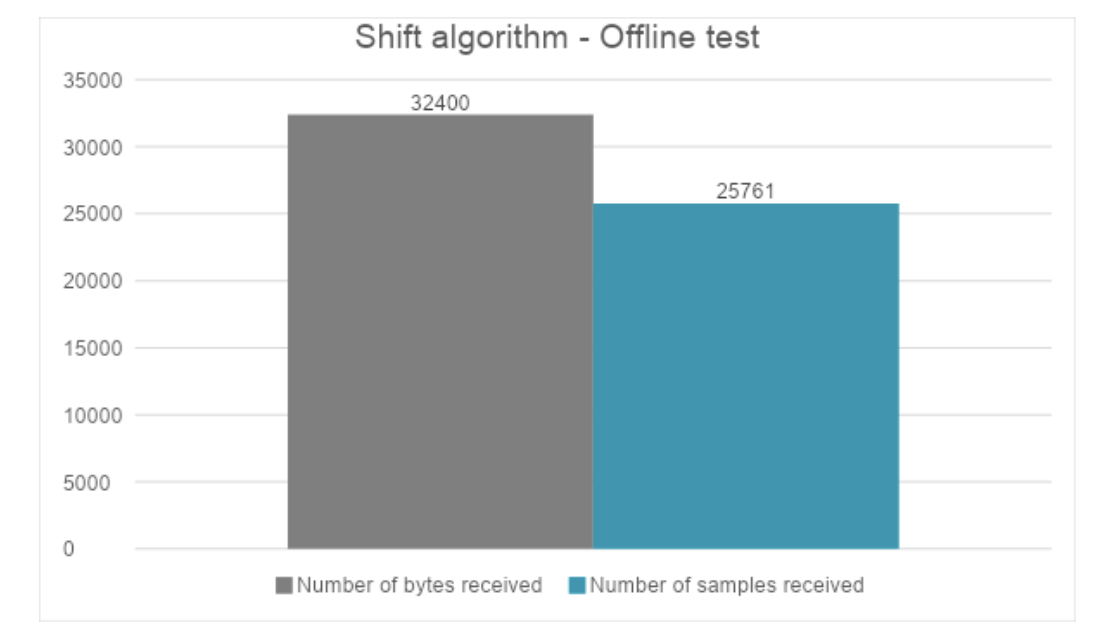
\includegraphics[scale=0.7]{Shift Algorithm/Screenshot 2024-07-22 at 22.31.45.png}
    \caption{Shift algorithm}
    \label{pairing_procedure_5}
\end{figure}

By making a comparison between the final number of samples received in both cases, the shift implementation guarantees an increase in received samples of 37.11. However, the shift algorithm is not limited to compression. Original samples need to be reconstructed once the central device has received all of the data in order to have full access to the information which comes from the ADC. To do that, a decompression algorithm has been implemented as well. The scheme, as before, is shown below:

\begin{figure}[H]
    \centering
    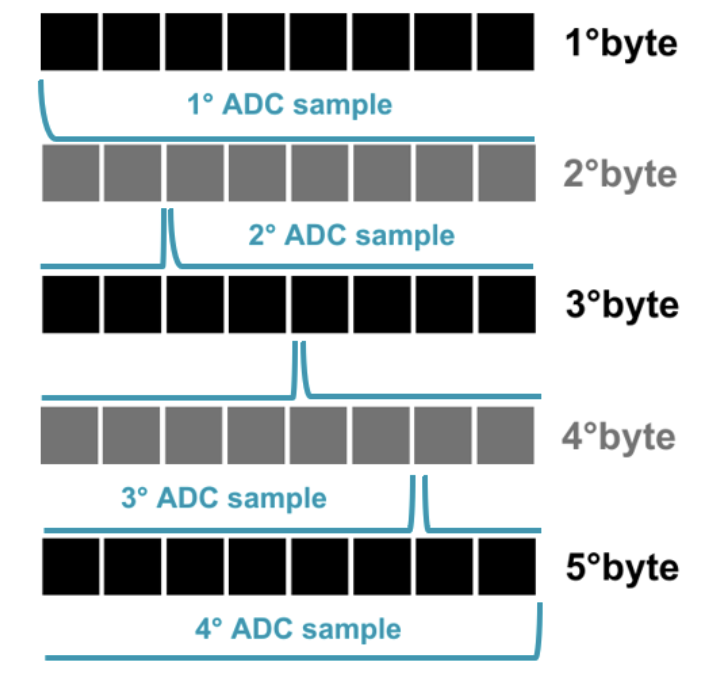
\includegraphics[scale=0.7]{Shift Algorithm/Screenshot 2024-07-22 at 22.31.56.png}
    \caption{Shift algorithm receiver side}
    \label{pairing_procedure_6}
\end{figure}

Differently from the peripheral side, the central device will receive data which are in byte, and needs to be decompressed. The procedure is composed of the following steps:
Firstly, the whole first byte is put together with the 2 most relevant bits of the second byte in order to reconstruct the first sample. Then, the second sample is formed by the 6 less relevant bits of the second byte, put together with the 4 most relevant bits of the third byte. The third sample is composed of the four most rightly positioned bits of the third byte together with the 6 most relevant bits of the fourth byte. The remaining bits of the fourth byte together with the whole fifth byte would constitute the fourth sample. As before, the whole procedure is periodic. In case of a full-sized BLE packet, this is repeated until 240 bytes have been processed. The last 4 bytes are simply coupled as it happened in the previous version of the firmware.

An example of the whole procedures of compression and decompression is shown below: 

\begin{figure}[H]
    \centering
    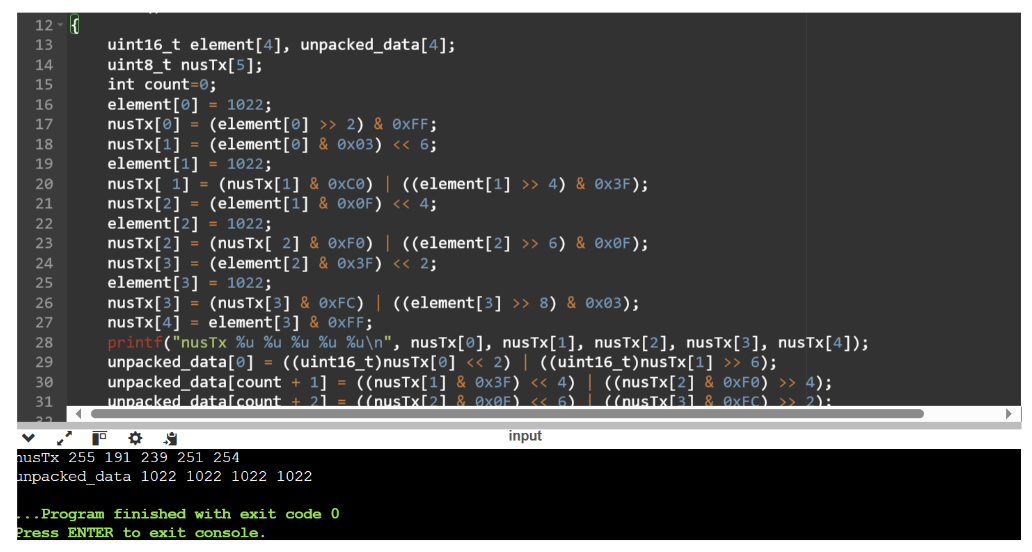
\includegraphics[scale=0.7]{Shift Algorithm/Screenshot 2024-07-22 at 22.32.05.png}
    \caption{Shift procedure example}
    \label{pairing_procedure_7}
\end{figure}

In the purposed example, vector elements act as the ring buffer which should contain the ADC samples. All of the fourth samples generated have the same value in this case which is 1022. This number has not been chosen randomly, but it is the maximum number that can be represented in binary using 10 bits, exception made for 1023 which is representable as a sequence of 10 bits 1. 1022 can instead be represented in binary language as 1111111110. The presence of the last zero is useful to understand whether or not the shift algorithm is operating correctly. Firstly, data are compressed, and bytes generated are saved into the \texttt{nusTx} vector, which is the one which simulates the storage of bytes. The values inside \texttt{nusTx} are then printed. To verify that these values are the ones expected, the whole steps previously explained are performed:
The first \texttt{nusTx} value should take the 8 most relevant bits of \texttt{element[0]}. In this case, all of the numbers inside elements are 1022, so the first 8 bits are 8 bits 1, which can be written in decimal as 255.
Then, the last two bits inside \texttt{element[0]} are put together with the 6 most relevant bits of \texttt{element[1]}, which implies that the second byte represents the number 10111111, which corresponds to 191.
The third step is made by combining the 4 less relevant bits of \texttt{element[1]} and the 4 most relevant bits of \texttt{element[2]}. This would result in 11101111, 239 in decimal.
The fourth step needs to put together the 6 less relevant bits of \texttt{element[3]} and the 2 most relevant bits of \texttt{element[3]}. The result is 11111011, which is 251.
The last step is done by simply taking the 8 less relevant bits of \texttt{element[3]}, which are 11111110, which corresponds to 254.
With this example, it has been shown that the firmware implementation of the algorithm works as expected. Finally, the inverse operation is performed as well, and values are printed. These values are correct for sure because the values of the generated samples were originally known, they correspond to 1022. In order to provide an example also of the decompression, however, all of the steps are explained anyway.
The first sample is reconstructed by putting together the whole first byte, 11111111, with the first two bits of the second one 10111111. This results in 1111111110, which is 1022.
The second one is composed of the 6 less relevant bits of the second byte, 10111111, and the 4 most relevant bits of the third byte 11101111. The result is again 1111111110.
The third sample is made by putting together the 2 most right positioned bits of the third byte, 11101111, and the 6 left positioned bits of the fourth byte, which is 11111011, resulting again in 1022.
Lastly, the fourth sample is composed of the 2 remaining bits inside the fourth byte and the whole fifth byte. The result is again 11111110 or 1022.

\subsection{Firmware Implementation: Offline Transmitter}

For what regards the firmware implementation, two functions are principally implied by the shift operations: \texttt{timer1\_handler} and \texttt{Spibuffprocess}. The first one is the function which is responsible for data generation, while the second one re-organizes the samples generated into bytes in order to make them ready to be sent.
The \texttt{timer1\_handler} function is quite similar to the previous version of the firmware, just a few changes became necessary. Firstly, the number of samples generated in order to reach a communication of 32400 bytes size should be incremented, according to the increase previously explained. To do that, the number of samples generated before putting the last value 65535 is no more given by $(\text{DATA TO SEND}-2) \cdot 2-1$, which would result in 16198, but this limit is instead substituted by:
\[
\text{n°samples for each packet} \times \text{n°full filled BLE packets} + \text{n°samples last packet}
\]
Which would result in 194*132+152=25760 samples. 
Because of this limit incrementation, a further modification of the \texttt{timer1\_handler} function became necessary. Because of the limit imposed by the RAM of the peripheral device, the ring buffer which contains all of the samples has a size of 16384. It can easily possible to see that the previous number of samples never exceeded the maximum number that the buffer could contain, causing no problems in the data generation process. 
With the shift algorithm, instead, due to the increased number of samples generated, this limit is reached and the behaviour that could happen is that some samples are lost because they have not been sent to the central device fast enough. In order to do that, a further condition has been added. In particular, the generation of new data and the consequent storage inside the ring buffer is allowed only if the data already in the buffer are less than 16200, which represents the 97.88 percent of the buffer. This condition guarantees that the buffer has enough free memory before being filled, and no wasting of information is implied. Ultimately, a further condition is added. In order to generate data which are as much as possible similar to the actual samples coming from the ADC, \texttt{CNT} maximum value has been posed to 1022, which is the maximum value that can be represented with 10 bits, exception made for 1023, where \texttt{CNT} is the variable which simulates the arrival of the samples.
As previously said, also the \texttt{Spibuffprocess} function has been modified. In detail, the function counts the number of samples actually inside the ring buffer. In the previous implementation, the data packing into bytes operation was performed if they were at least \texttt{senseback\_MTU/2}, which corresponds to 122 samples. With the shift implementation, however, the number of samples that can be packed in 244 bytes is no more 122, but it is 194. This value is stored in the variable \texttt{ELEMENTS\_IN\_A\_CYCLE}, which represents the new lower limit of samples. If there are at least 194 samples in the buffer, the generation of a full-sized BLE packet of 244 bytes can be performed. This is done as shown before, by performing shift operations until the bytes generated are 240. Each time a cycle is completed, four new samples are taken from the ring buffer. The last four bytes are generated as done in the previous firmware version. Ultimately, the last packet should be processed. This process is done when the ring buffer contains at least one element and the total number of bytes that need to be sent to guarantee a communication of 32400 bytes is less than 244. Then, a fictitious variable is used as a counter to represent the number of samples taken and processed from the ring buffer. Until this counter has not reached the last 4 samples inside the buffer, the shifting process is performed. The last values would not be shifted. This last choice has been made in order to assure that the last value 65535 would not be shifted, where this value is used to signal that the end of the communication is reached. 

\subsection{Firmware Implementation: Offline Receiver}

In order to avoid a possible impact on the speed of the receiving packets process, in the receiver code data are unpacked when communication ends. To do that, the new function \texttt{process\_senseback\_data} has been implemented. This function is called when the central device has received the last bytes 255 and 255. To this function, the whole buffer which contains the bytes received is passed. The function would then decompress the data. For the purpose of an offline test, since the number of bytes and samples that would be received is known, the vector which would contain the unpacked data has a fixed size, which is 25761, as the number of samples. Then, the process of decompression is done as many times as the number of BLE packets received, exception made for the last one. For the last packet, the process is the same, the only difference resides in the last two bytes, which are the only ones that would be put together without the decompression algorithm.

\subsection{Firmware Implementation: Online Transmitter}

For what regards the function \texttt{timer1\_handler}, the only modification done for the online case is the maximum value of the \texttt{CNT} variable, which has been posed to 1022 as for the offline case. The \texttt{Spibuff} function is also quite equivalent to the one implemented for the offline case, the only differences are the ones relative to the fact that the communication has not a fixed size, and so they have already been explained for the previous version of the firmware. In order to show the difference in terms of informative throughput when the shift algorithm is adopted, a further variable \texttt{count\_zeros} has been used. This acts as a counter to count how many empty bits are present when the shift algorithm is adopted and when it is not.

\subsection{Firmware Implementation: Online Receiver}

Compared to the offline receiver case, the online one implicates a small further challenge, which is due to the fact that the number of packets is not known a priori. To compute it and consequently know how many packets need to be shifted and how, the idea is to use the following equation:
\[
\text{n° BLE packets} \approx \frac{\text{n° bytes received}}{\text{maximum BLE packet size}}
\]
to compute the number of BLE packets and using the rest given by this operation to know the size of the last BLE packet. Once these values are known, the whole procedure of unpacking can be performed.
A limit that this approach presents is due to the size of the RAM, which is not enough to actually perform the unpacking process. Future implications of this process should imply a study on how it could be possible to save some memory in the microcontroller, and how fast the packing and the unpacking processes are.


\section{Firmware Security Implementation}
As explained in previous sections, security implementation is fundamental both from the normative point of view and for guaranteeing privacy and safety of the patient, especially for those communications which are wireless, and can then easily be sniffed. In order to have a chance for the device to be approved, the highest level of security that a device supports should be implemented. Considering that the communication is point to point, because just two devices are involved, and that the devices support the most updated Bluetooth low energy versions, this level corresponds to mode 1 level 4, which implies the involvement of Bluetooth Low Energy Secure Connection.

To implement this, the steps are similar in both the central and peripheral devices. Specifically, \textit{Peer Manager} is involved. Peer manager is used in the context of BLE in order to manage all tasks related to security, such as encryption, pairing, or bonding. When a bonding procedure is required, the peer manager stores the Long-Term Keys into the flash memory and the same is for GATT data. Some of the advantages in the peer manager implementation are the following:

\begin{itemize}
    \item It can be used for both central and peripheral roles.
    \item It works autonomously, including possible reattempts.
    \item It is easy to use.
    \item It is modular, making it easy to implement possible new features.
    \item It saves energy. By storing GATT data, it saves the need for packet exchange.
    \item When a change in the GATT database occurs, Peer Manager is responsible for sending an indication that this event occurred to all of the bonded devices.
    \item Peer Manager also solves the random resolvable private address.
\end{itemize}

The Peer Manager architecture is shown below:

\begin{figure}[h]
    \centering
    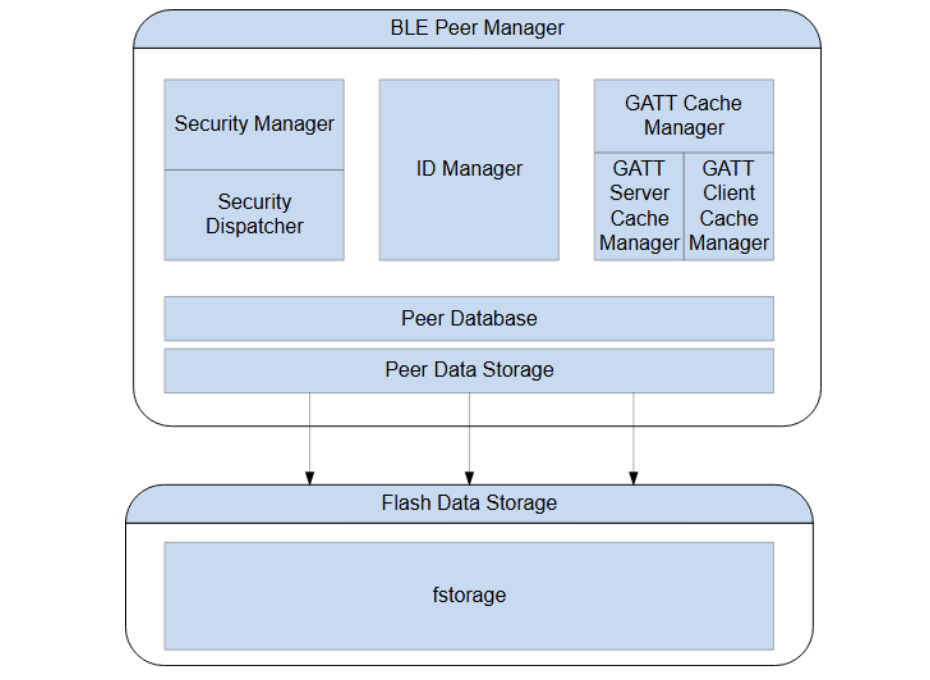
\includegraphics[scale=0.3]{Firmware_security/Screenshot 2024-07-22 at 22.33.12.png}
    \caption{Peer manager}
    \label{firm_sec_1}
\end{figure}

All the parts which compose the peer manager are shown in Figure~\ref{firm_sec_1}. Specifically, the first section regards the security manager and dispatcher. This is responsible for managing all the steps in the security process, based on the requirements of the involved applications. These steps include the creation of a secure connection by communicating with the SoftDevice, saving and deleting the proper keys, and performing the pairing procedure. The module is divided into two components: the Security Manager and the Security Dispatcher. The first one is responsible for storing security parameters, monitoring the current state, and managing the pairing process. The Security Dispatcher connects with the SoftDevice and the flash to perform the actual pairing procedure.

The second one is the ID manager. This module monitors connected peers and recognizes them using various types of IDs. It is also able to check whether different IDs are used for the same peer and whether a bonding procedure has been performed. When this is the case, it can also ask for the connection handle.

The GATT cache manager has three main functionalities. It stores the CCCDs, which stand for Client Characteristic Configuration Descriptor, it distributes the notifications when a change in the services occurs, and it could store ATT databases.

Ultimately, Peer Database and Peer Data storage respectively hold stored data for the peer IDs and provide an interface between the Peer Database and the Flash Data storage module.

In detail, the following steps explain how security features have been implemented for the intended BLE connection. The majority of the changes are common for both the receiver and the transmitter, and there is no difference in terms of online and offline codes. The only differences between central and peripheral firmware are relative to the roles and would be shown later in this section.

Firstly, the connection procedure is performed. This presents no changes compared to the previous implementation. Once this is done, before the pairing procedure occurs, the two devices should configure the required security features. This is done in the function \texttt{peer\_manager\_init}, which first initializes the Peer Manager module through the function \texttt{pm\_init} and then sets the security parameters for the BLE connection. In particular, the features that can be chosen are relative to the following flags:

\begin{itemize}
    \item \textbf{Security parameters bond}: by setting this flag as true, the device knows that, after the pairing procedure, a bonding one should also be performed. For the purpose of this application, this feature is implemented. This is because it could happen that the Senseback device goes into standby mode, possibly causing a disconnection between implanted and external devices. This is done to save battery life, and the bonding procedure avoids that the whole pairing procedure is performed each time from the beginning.
    \item \textbf{Security parameters MITM}: this flag should be set in cases where protection against a possible Man In The Middle attack is required. Generally speaking, this protection is advised, but it requires that both devices have input/output capabilities. In the Senseback context, the choice was to implement a Just Works procedure since the actual capabilities of the Senseback device were not properly known. In future implementations, this protection can easily be implemented just by setting this flag to true in both devices, assuring that both have the capabilities to support this feature.
    \item \textbf{Security parameters LESC}: this field is responsible for the implementation of Low Energy Secure Connection, which guarantees the highest level of security, which is level 4. This flag has been set to 1.
    \item \textbf{Security parameters keypress}: this establishes whether or not the intended device has input capabilities. Specifically, if the user can input a possible password through a keyboard. Again, since Just Works association mode has been selected, this parameter has been set to 0 in both devices.
    \item \textbf{Security parameters input/output capabilities}: this field should be set to true if the intended device has both input and output capabilities. Without this flag, even if the MITM flag is true, the protection against a Man In The Middle attack is not guaranteed. For the Just Works purposes, this flag is not necessary.
    \item \textbf{Security parameters Out of Band}: this flag indicates that the intended association mode should be Out of Band. So, the exchange of keys can, for example, be performed using another kind of communication such as NFC. This is the most secure association mode. It is not required for Just Works purposes.
    \item \textbf{Security parameters min/max key size}: these parameters establish what should be the minimum and maximum sizes of the password used for association. Even if a proper password has not been thought for the security process implemented, these parameters have been set to 7 and 16 respectively, which guarantee a quite long and consequently consistent password.
    \item \textbf{Security parameters enc}: This field stands for ``encryption key''. When set to 1, it indicates that the local device will distribute its encryption key to the peer device during the pairing process. The encryption key is used to establish a secure encrypted connection.
    \item \textbf{Security parameters identity key}: When set to 1, it indicates that the local device will distribute its identity key to the peer device during the pairing process. The identity key is used to identify the device and for privacy features in BLE.
    \item \textbf{Security parameters peer encryption}: it indicates that the peer device will distribute its encryption key to the local device during the pairing process.
    \item \textbf{Security parameters peer identity key}: it indicates that the peer device will distribute its identity key to the local device during the pairing process.
\end{itemize}

These last four parameters have all been set to true to have a proper security process. To have the functionality correctly implemented, both devices should have set the same parameters. For example, if one of the two requires MITM protection and the other one does not, this feature would not be present during the pairing procedure. These parameters become effective once the functions \texttt{pm\_sec\_params\_set} and \texttt{pm\_register} are called. A further parameter that has not been explained above is the LESC debug mode. This allowed the developer to sniff the packets even if LESC is implemented. However, this functionality has been removed from nrf5 SDK version 15.0, to avoid that a possible product is released into the market with this functionality enabled, which should be used only for developing purposes, making the BLE communication vulnerable to possible attacks. Because of this, when LESC security is implemented, it is not possible to sniff packets. Therefore, the number of retransmissions cannot be checked with this implementation.

After the parameters are set, the function \texttt{pm\_evt\_handler} is called to handle security events. This function calls itself two other functions which are \texttt{pm\_handler\_on\_pm\_evt}, which is responsible for logging peer manager possible events, it starts encryption in cases where the bonding procedure is implemented, and manages possible fatal errors. The other function is \texttt{pm\_handler\_flash\_clean}, which is responsible for maintaining some room in the flash memory that would be used by the peer manager. Ultimately, the function \texttt{pm\_evt\_handler} manages two events: the first one is triggered each time a change in peer data is successfully performed, such as storing or updating. This event is present only in the firmware implementation of the peripheral device. Once triggered, it calls the function \texttt{advertising\_start}. The second event is common for both receiver and transmitter. It is triggered when the bonding procedure has been performed. Even though the event is common in both devices, they manage it differently. The peripheral, in fact, just logs that the bonding procedure has been successfully performed. The central device, instead, starts scanning once this is done.

Another common function which is added to both the main files for the central and peripheral devices is \texttt{nrf\_ble\_lesc\_request\_handler}. This function is called in the main function, and it is responsible for responding to a DH key request and generating the DH keys. It returns different codes based on the success or failure of the intended event.

A further modification, which is relative only to the peripheral device, regards the function \texttt{advertising\_start}. This function would not only be responsible for starting the BLE advertising procedure, but it also would delete all the stored bonds when necessary.

Ultimately, in the previous implementation, the GAP response to a security request event was to indicate that the used device did not have any security feature. Clearly, this event has been removed to allow the device to perform the security procedure. When a LESC DHKEY request or an AUTH DHKEY request event occurs, the triggering of them is simply logged.

These are the only changes done in the main code necessary to implement LESC in central and peripheral devices. However, these changes would not be effective if relative changes in the configuration files are not implemented. Some of them are common in both peripheral and central devices, others are different because they are based on the specific role of the devices. They are briefly explained below:

\begin{itemize}
    \item \textbf{NRF\_BLE\_LESC\_ENABLED}: this flag enables Low Energy Secure Connection usage.
    \item \textbf{PEER\_MANAGER\_ENABLED}: this allows the enabling of the peer manager module.
    \item \textbf{PM\_CENTRAL\_ENABLED}: this is specific for the central device; it enables the specific peer manager functionalities.
    \item \textbf{PM\_LESC\_ENABLED}: it allows the function call \texttt{nrf\_ble\_lesc\_request\_handler()} to respond to possible events related to Low Energy Secure Connection.
    \item \textbf{NRF\_CRYPTO\_BACKEND\_NRF\_HW\_RNG\_ENABLED}: this is a configuration macro used to enable or disable the hardware random number generator (RNG) backend within the cryptographic library.
    \item \textbf{NRF\_CRYPTO\_BACKEND\_OBERON\_ENABLED}: it enables the Oberon backend, which is an implementation of the Elliptic Curve Digital Signature Algorithm (ECDSA) and Elliptic Curve Diffie-Hellman (ECDH) based on the Oberon Cryptography.
    \item \textbf{NRF\_CRYPTO\_RNG\_STATIC\_MEMORY\_BUFFERS\_ENABLED}: it allows the usage of static memory buffers for context and temporary init buffer.
    \item \textbf{NRF\_CRYPTO\_RNG\_AUTO\_INIT\_ENABLED}: it allows the automatic initialization of the RNG module once \texttt{nrf\_crypto} has been initialized.
    \item \textbf{NRFX\_RNG\_ENABLED}: used to enable the Random Number Generator (RNG) peripheral driver. Random numbers are crucial for cryptographic operations, secure communications, and other applications requiring randomness.
    \item \textbf{RNG\_ENABLED}: it enables the Random Number Generator (RNG) functionality.
    \item \textbf{FDS\_ENABLED}: it enables the Flash data storage module.
    \item \textbf{NRF\_FSTORAGE\_ENABLED}: it is a configuration setting used to enable the fstorage module, which provides an abstraction layer for flash storage.
\end{itemize}

The following pictures illustrate the difference in terms of logs after the connection is performed when security is implemented and when it is not, for both central and peripheral device roles. It is possible to see, thanks to the logs, all of the steps related to security implementation which have been explained above, and when they are exactly performed in the pairing and bonding procedures.

\begin{figure}[h]
    \centering
    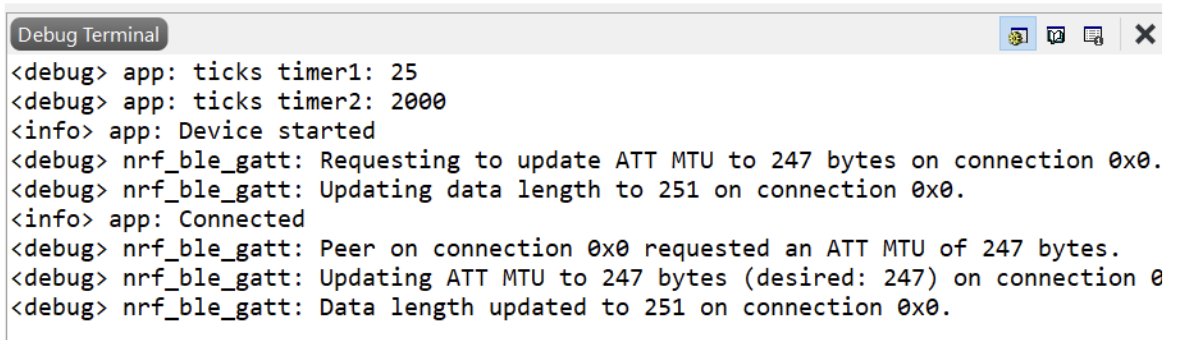
\includegraphics[scale=0.3]{Firmware_security/Screenshot 2024-07-22 at 22.33.24.png}
    \caption{Peripheral firmware without security}
    \label{firm_sec_2}
\end{figure}

\begin{figure}[h]
    \centering
    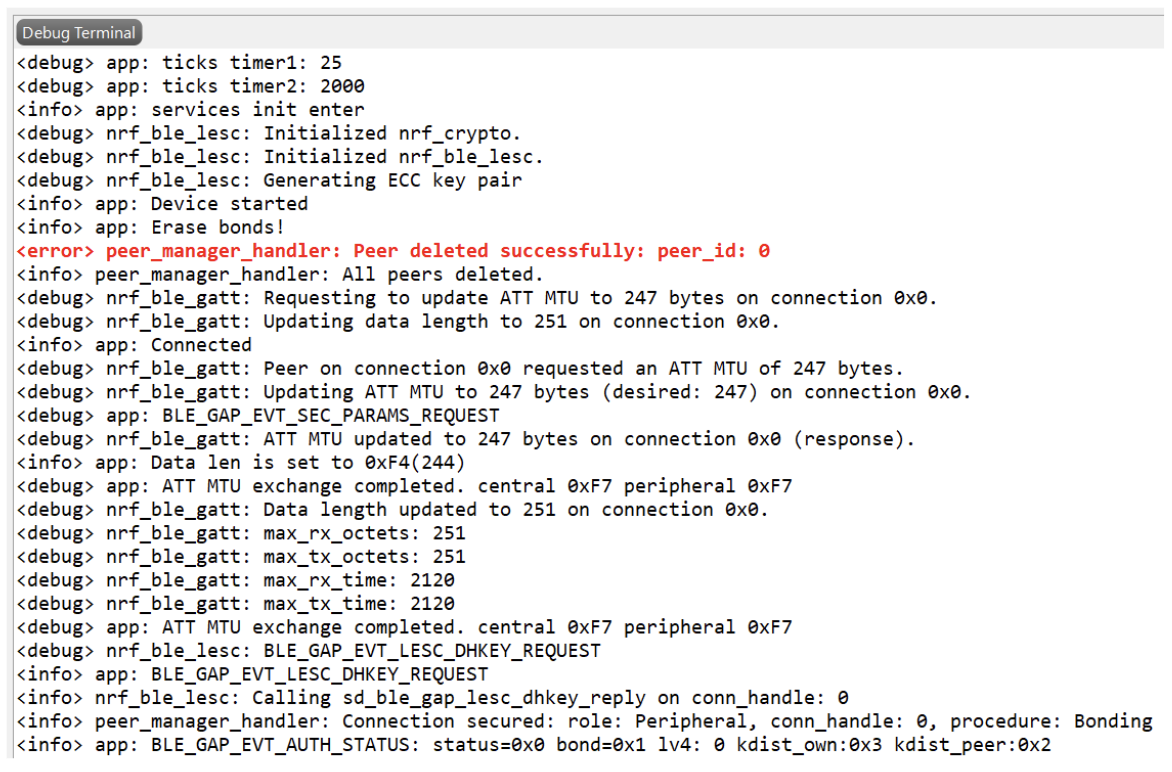
\includegraphics[scale=0.3]{Firmware_security/Screenshot 2024-07-22 at 22.33.31.png}
    \caption{Peripheral firmware with security}
    \label{firm_sec_3}
\end{figure}

\begin{figure}[h]
    \centering
    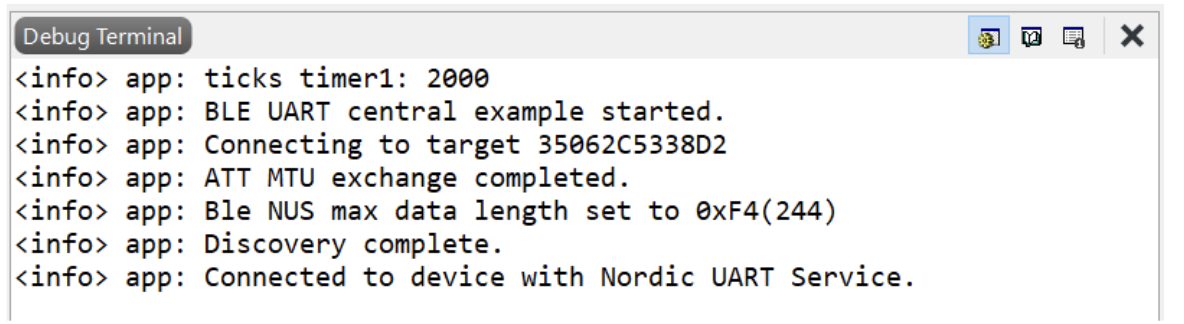
\includegraphics[scale=0.3]{Firmware_security/Screenshot 2024-07-22 at 22.33.37.png}
    \caption{Central firmware without security}
    \label{firm_sec_4}
\end{figure}

\begin{figure}[h]
    \centering
    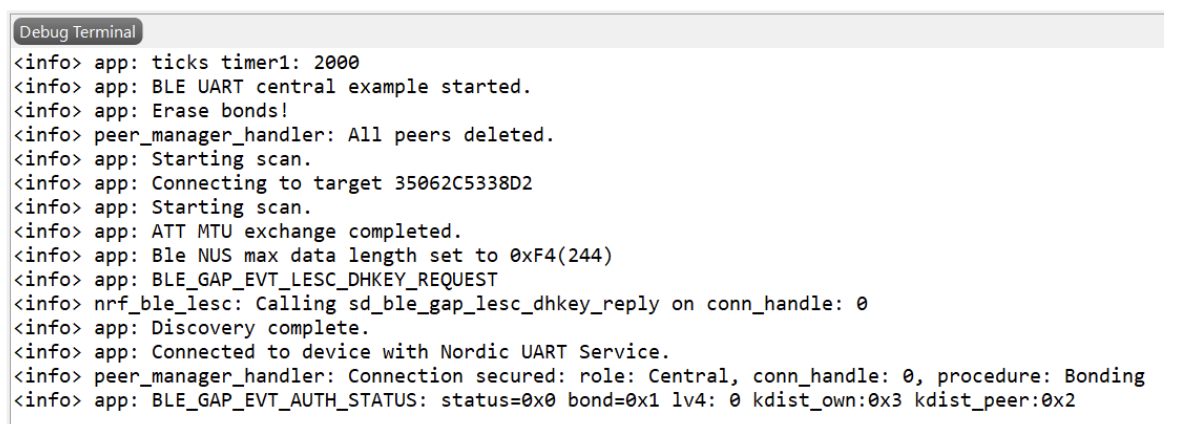
\includegraphics[scale=0.3]{Firmware_security/Screenshot 2024-07-22 at 22.33.43.png}
    \caption{Central firmware with security}
    \label{firm_sec_5}
\end{figure}

\\
\section{Theoretical throughput computation}

Theoretical throughput computation provides an idea on which is the maximum speed than the BLE communication can reach, taking into account some factors, such as latency, which is not considered in the ideal PHY, whose values could be 1 Mbps or 2 Mbps. In order to make a correct calculation, different parameters should be considered basing on different condition in the experimental setups, such as whether or not encryption is enabled, or which is the chosen PHY. As a consequence, all the possible cases are considered for the different intended usages.

Firstly, some common assumptions are made:
\begin{itemize}
    \item Theoretical throughput is computed for unidirectional communications: from peripheral to central and not vice versa.
    \item Because of the previous assumption, the exchanged packets, which go from central device to peripheral one, are empty.
    \item Write without response mode is used. This would maximize the maximum throughput achievable, because there is no time considered for waiting for a response.
    \item Between the exchange of two packets, an inter frame space (IFS) of 150$\mu$s is considered.
\end{itemize}

Once these assumptions are made, it is possible to compute the time needed for a single packet exchange. Specifically, the time required is computed by summing the time needed to exchange a full packet size from peripheral to central, the time needed for the exchange of an empty packet, and the IFS between these two, as reported in Equation \ref{eq:packet_exchange}:
\begin{equation}
t_{\text{packet exchange}} = t_{\text{empty packet}} + \text{IFS} + t_{\text{full size packet}} + \text{IFS}
\label{eq:packet_exchange}
\end{equation}

In order to compute the time needed to send an empty and a full-size packet, different conditions should be analysed.

\subsection*{Case 1: No Security Features, PHY = 2 Mbps}

First case refers to those cases in which security features such as encryption are not implemented and PHY is set to 2 Mbps, such as the previous implementation or the case with shift algorithm, but without security.

\begin{figure}[h]
    \centering
    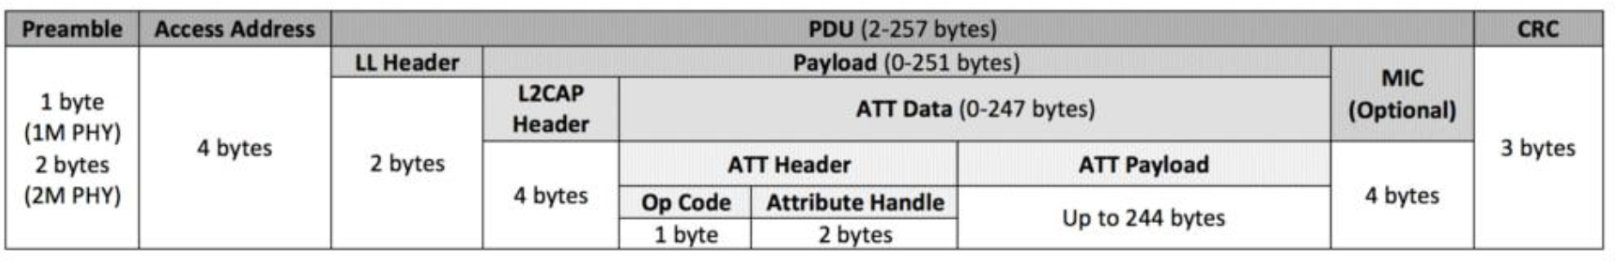
\includegraphics[scale=0.3]{theoretical_throughput.png}
    \label{theoretical_1}
    \caption{Packet structure}
\end{figure}

Since encryption is not enabled, then the MIC field is not present. Moreover, since PHY is equal to 2 Mbps, preamble would be 2 bytes size. Considering this, it is now possible to compute the sizes of empty packets as follows:
\begin{equation}
\text{size}_{\text{empty packet}} = \text{Preamble} + \text{Access Address} + \text{LL Header} + \text{CRC} = 11 \text{ bytes}
\label{eq:size_empty_packet}
\end{equation}

The size of a packet containing data is, instead:
\begin{equation}
\text{size}_{\text{full size packet}} = \text{size}_{\text{empty packet}} + \text{Payload} = 262 \text{ bytes}
\label{eq:size_full_size_packet}
\end{equation}

Defined these parameters, it is possible to compute the time needed to send an empty and a full size packet by dividing them for the chosen PHY (2 Mbps).
\begin{equation}
t_{\text{empty packet}} = \frac{\text{size}_{\text{empty packet}}}{\text{PHY}} = 44 \mu \text{s}
\label{eq:t_empty_packet}
\end{equation}
\begin{equation}
t_{\text{full size packet}} = \frac{\text{size}_{\text{full size packet}}}{\text{PHY}} = 1048 \mu \text{s}
\label{eq:t_full_size_packet}
\end{equation}

Now it is possible to compute the time needed for a packet exchange as reported in Equation \ref{eq:packet_exchange}.
\begin{equation}
t_{\text{packet exchange}} = 1048 \mu \text{s} + 150 \mu \text{s} + 44 \mu \text{s} + 150 \mu \text{s} = 1392 \mu \text{s}
\label{eq:packet_exchange_case1}
\end{equation}

Considering a connection interval of 50 ms, the number of packets exchanged during a single connection event is:
\begin{equation}
\text{number of packets} = \frac{\text{CI}}{t_{\text{packet exchange}}} = 35
\label{eq:number_of_packets_case1}
\end{equation}

Finally, the throughput is computed by multiplying the number of bits which contains information times the number of packets per CI, dividing for the time needed for those connection event.
\begin{equation}
\text{Throughput} = \frac{\text{number of packets} \times \text{ATT payload}}{\text{CI}} = 1366 \text{ Mbps}
\label{eq:throughput_case1}
\end{equation}

\subsection*{Case 2: Security Features, PHY = 2 Mbps}

The computation of theoretical throughput when security features are implemented is slightly different from the previous case due to the additional MIC header, visible in Figure 1. As a consequence, the formulas for the computation of the sizes of empty and full-size packets change accordingly:
\begin{equation}
\text{size}_{\text{empty packet}} = \text{Preamble} + \text{Access Address} + \text{LL Header} + \text{CRC} + \text{MIC} = 15 \text{ bytes}
\label{eq:size_empty_packet_case2}
\end{equation}
\begin{equation}
\text{size}_{\text{full size packet}} = \text{size}_{\text{empty packet}} + \text{Payload} + \text{MIC} = 266 \text{ bytes}
\label{eq:size_full_size_packet_case2}
\end{equation}

According to Equation \ref{eq:t_empty_packet} and Equation \ref{eq:t_full_size_packet}, the two time values for this case are: $t_{\text{empty packet}} = 60 \mu \text{s}$ and $t_{\text{full size packet}} = 1064 \mu \text{s}$.

By repeating the same process done in Case 1, the results are the following: $t_{\text{packet exchange}} = 1424 \mu \text{s}$, $\text{number of packets} = 35$.

As a consequence, throughput is the same as in Case 1. Security features should not have an impact on the speed.

\subsection*{Case 3: No Security Features, PHY = 1 Mbps}

This case is considered because it is the one used for the approach with one board and one PC as external unit. Since security features are not enabled, the size of the packets is the same as in Equation \ref{eq:size_empty_packet} and in Equation \ref{eq:size_full_size_packet}. The difference resides in the computation of the time needed to exchange the packets, since PHY is 1 Mbps in this case.

The results are then: $t_{\text{empty packet}} = 88 \mu \text{s}$ and $t_{\text{full size packet}} = 2096 \mu \text{s}$.

The total time is:
\begin{equation}
t_{\text{packet exchange}} = 2484 \mu \text{s}
\label{eq:packet_exchange_case3}
\end{equation}

The number of packet changes accordingly:
\begin{equation}
\text{number of packets} = 17
\label{eq:number_of_packets_case3}
\end{equation}

Finally, the theoretical throughput is equal to 663.68 Mbps.

\section{Multicentral Implementation}
As explained in previous sections, the user can control the communication beginning and end through UART communication. Thanks to this, the user can send commands, which are first sent to central devices and then to the peripheral through Bluetooth. The whole process is shown in Figure 4.14.

\begin{figure}[H]
    \centering
    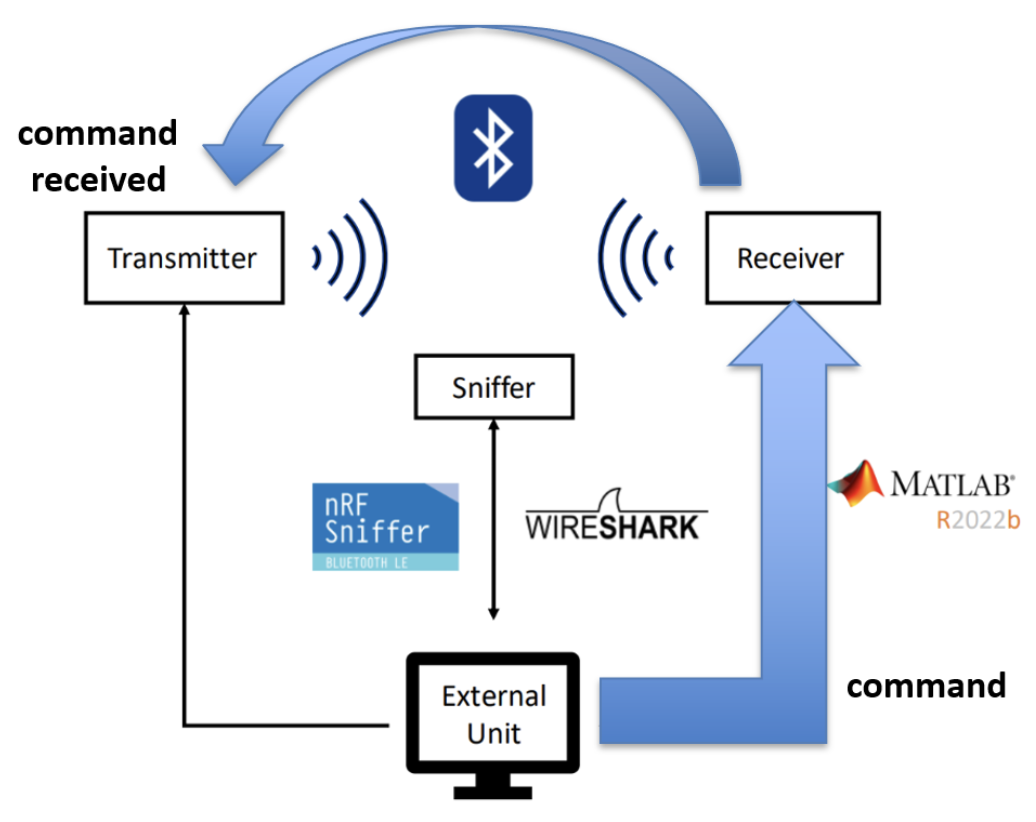
\includegraphics[scale=0.5]{Multicentral/1.png}
    \caption{User command sending procedure in previous implementation}
    \label{multicentral_1}
\end{figure}

In the current Senseback device, the wires used in the previous implementation to send commands are not present. This makes it impossible to control the communication as in the previous version of the firmware. To solve this problem, a new way to send commands to control the communication has been devised. The proposed idea is shown in Figure 4.15.


\begin{figure}[H]
    \centering
    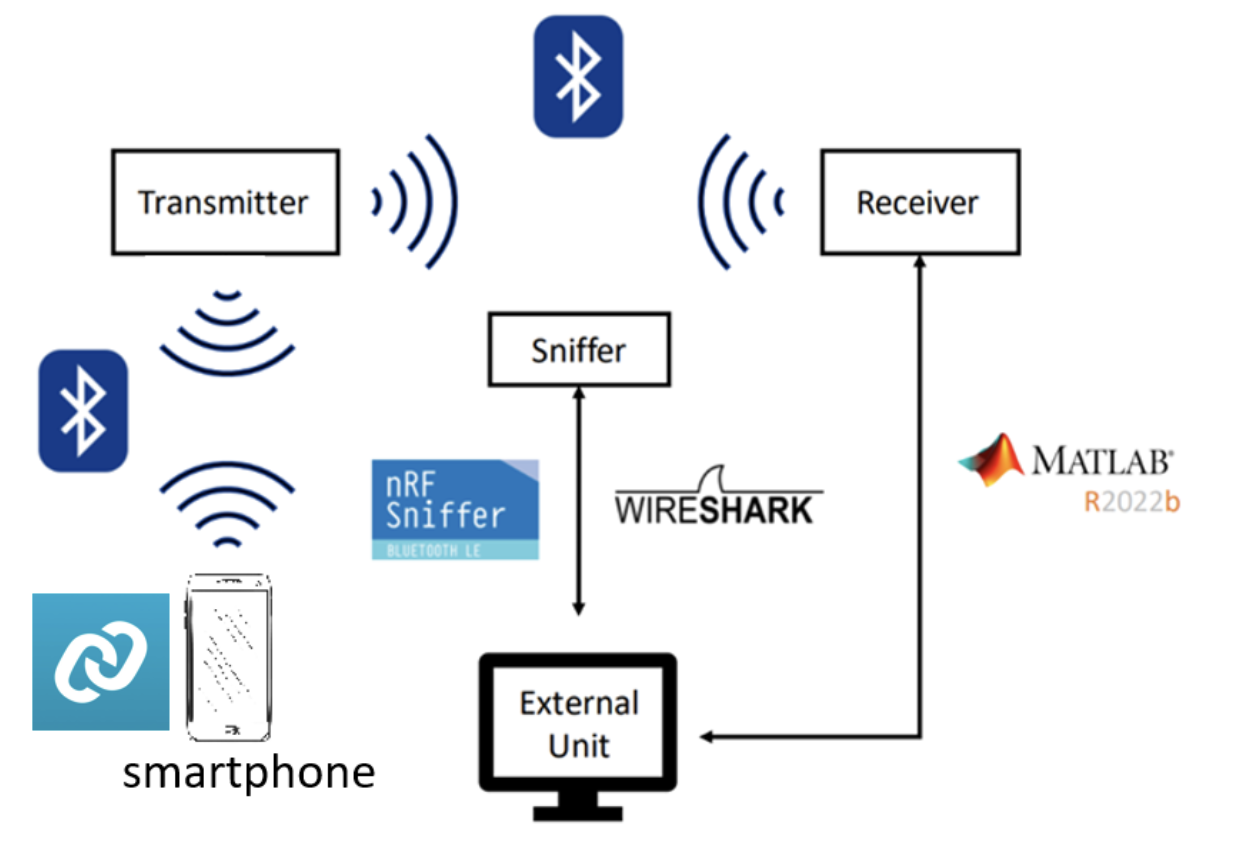
\includegraphics[scale=0.5]{Multicentral/2.png}
    \caption{Multicentral implementation}
    \label{multicentral_2}
\end{figure}

The new implementation requires the involvement of two central devices, which is why it is called multicentral. The peripheral device would not only be connected to the board that should receive data, but also to another device whose purpose is to send the START, STOP, and RESET commands. This avoids the need for UART command sending and allows the peripheral device to receive commands through Bluetooth as before, but from a second device this time.

The second central device chosen is a smartphone. This choice allows the user to utilize the nRF Connect for Mobile app developed by Nordic Semiconductors ©. This app is available for both iOS and Android smartphones and is a useful tool to control Bluetooth Low Energy communications between devices. The app can also be used for the peripheral role on Android devices, though this is not the purpose of this implementation.

Before explaining how the final communication works when the multicentral setup is completed, the following section will explain how this has been implemented in the firmware.

\subsubsection{Receiver Firmware Multicentral}
Specifically, in the receiver code of the firmware, only a few differences are present. The first one relates to the configuration file. In particular, the \texttt{NRF\_SDH\_BLE\_CENTRAL\_LINK\_COUNT} and \texttt{NRF\_SDH\_BLE\_TOTAL\_LINK\_COUNT} values have been changed from 1 to 2. These define the number of central devices present in the application and the total number of simultaneous connections, which are both two in this case. Due to these changes, more RAM memory needs to be allocated compared to the previous implementation. Segger provides an easy way to change the settings of the project the developer is working on. The procedure is shown in Figure 4.16.

\begin{figure}[H]
    \centering
    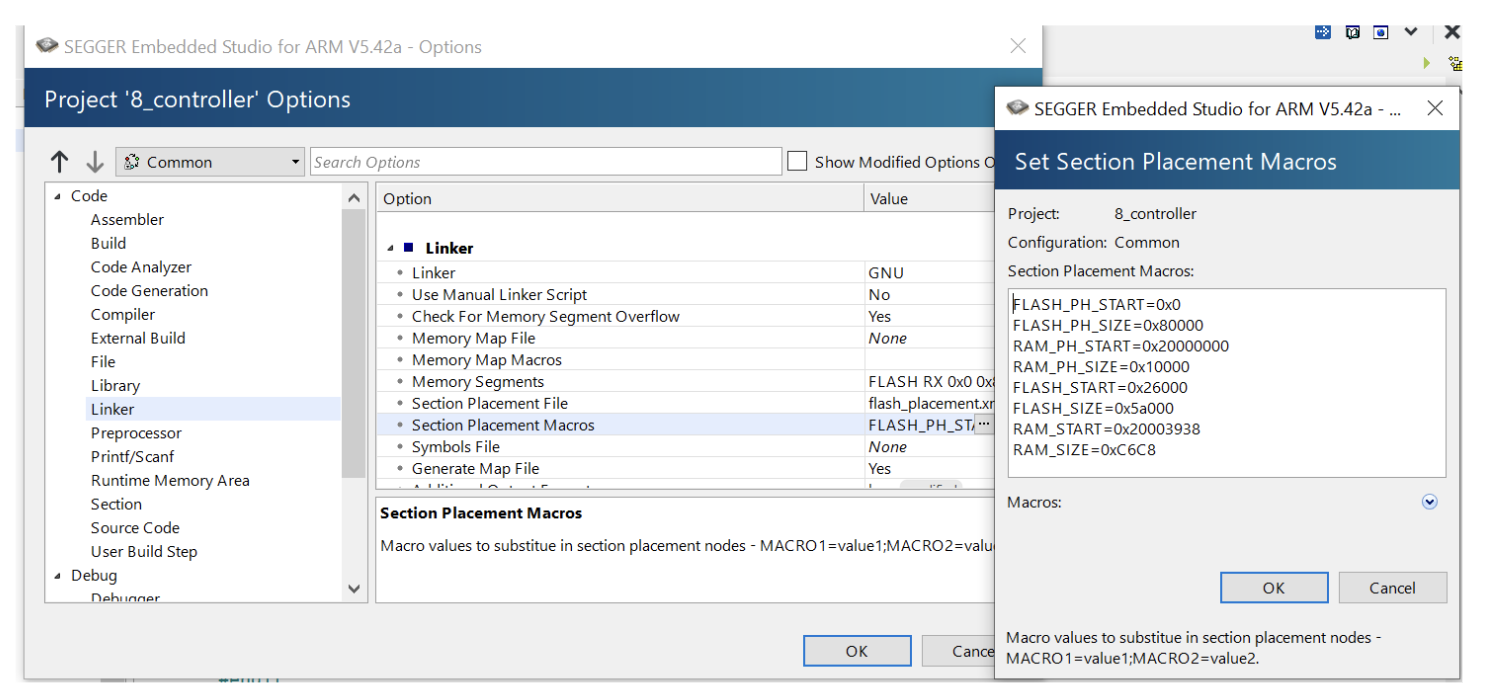
\includegraphics[scale=0.5]{Multicentral/3.png}
    \caption{Procedure to allocate memory in Segger}
    \label{multicentral_3}
\end{figure}

Specifically, in the Section Placement Macros, it was required to change the RAM START and RAM SIZE values. The minimum values required are directly shown to the user when the application is debugged. An example of this is shown in Figure 4.17.

\begin{figure}H]
    \centering
    \includegraphics[scale=0.6]{Multicentral/4.png}
    \caption{Memory allocation error in Segger}
    \label{multicentral_4}
\end{figure}

The other difference regards the main file. It is related to when the end of the communication should occur. In the previous implementation, this happened when both the last two bytes received were 255 and the \texttt{end\_transmission} variable was set to true, which means the STOP command was received. In the multicentral case, this last condition could not be verified since the STOP command is directly sent to the peripheral device. For implementations without shift, the last condition can simply be deleted, as the only bytes with a value of 255 would be the last ones, making the first condition sufficient. When shift is implemented, some bytes might have a value of 255 even if they are not the last ones, which could prematurely end the byte receiving process. To avoid this, a further value of 15 has been added. The receiving process correctly ends when the last three bytes are 255, 255, and 15. This further condition ensures that the last three values in the buffer are the expected ones. The value 15 was chosen randomly and can be substituted with any value except 255.

\subsubsection{Transmitter Firmware Multicentral}
For the transmitter code, the steps previously explained have already been performed, except the value to be changed is \texttt{NRF\_SDH\_BLE\_PERIPHERAL\_LINK\_COUNT} due to the different role. Further modifications regard the main file, which needs to manage two simultaneous connections instead of just one. The specific modifications are briefly explained below.

Firstly, NUS and QWR module definitions should account for the two simultaneous connections. Once these are defined, the \texttt{notification\_send} function, which sends data to the central device, should indicate to which device data should be sent. The connection handle is no longer singular but two, distinguished using the QWR module syntax \texttt{m\_qwr[0].conn\_handle} for the first and \texttt{m\_qwr[1].conn\_handle} for the second one. The best choice is to use the second board as the first central device and the smartphone as the second one, ensuring that the smartphone can reconnect if a disconnection event occurs. If the smartphone is treated as the first central device and a disconnection occurs, the board identified as the second central device becomes the first one, causing the peripheral to send data to the wrong device. For the multicentral and security features code, the smartphone is used as the first central device because it connects faster. This prevents simultaneous board-smartphone and board-board connections, which could cause the central board to enter a faulty error state.

\begin{figure}[H]
    \centering
    \includegraphics[scale=0.6]{Multicentral/5.png}
    \caption{Faulty error state central board}
    \label{multicentral_5}
\end{figure}

Other modifications handle connection and disconnection events separately. For example, the \texttt{on\_conn\_params\_evt} function manages possible connection errors by disconnecting the respective device. Managing these separately ensures that an error in one connection does not affect the other. Two additional functions, \texttt{on\_connected} and \texttt{on\_disconnected}, manage the respective GAP events previously handled by the \texttt{ble\_evt\_handler} function.

In the \texttt{on\_connected} function, the number of links established by the peripheral device is counted using the \texttt{ble\_conn\_state\_peripheral\_conn\_count} function. For each established link, a connection handle is assigned and logged. The PHY value is set to 2Mbps for the connection. If the number of links is less than the maximum value of two, more connections can be established, and the \texttt{advertising\_start} function is called.

The \texttt{on\_disconnected} function works similarly by counting the established links, setting the connection handle that triggered the disconnection to invalid, and calling the \texttt{advertising\_start} function if more connections can be established.

Finally, the \texttt{gatt\_evt\_handler} function, responsible for managing GATT events, updates the MTU if the event is an MTU update request from the device receiving data.

\subsubsection{Command Sending Process}
The procedure to send data through the smartphone is shown below. Firstly, the user should enable Bluetooth on the smartphone and open the nRF Connect app for mobile. The app will start scanning for nearby advertising Bluetooth devices.

\begin{figure}[H]
    \centering
    \includegraphics[scale=0.6]{Multicentral/6.png}
    \caption{nRF Connect scanning for devices}
    \label{multicentral_6}
\end{figure}

The app offers various features, including a peripheral mode, which is not used in this case. Default settings are sufficient for this purpose. The app shows the names of advertising devices and their power in dBm, allowing the user to connect with them. When the user clicks “Connect,” the app shows the following state:

\begin{figure}[H]
    \centering
    \includegraphics[scale=0.6]{Multicentral/7.png}
    \caption{nRF Connect connected state}
    \label{multicentral_7}
\end{figure}

By clicking on “Senseback” after connecting, the app shows different menus. The first menu relates to advertisements, showing a chart of the advertising power, the device name and features, and packet reception details.

\begin{figure}[H]
    \centering
    \includegraphics[scale=0.6]{Multicentral/8.png}
    \caption{nRF Connect advertisements menu}
    \label{multicentral_8}
\end{figure}

\begin{figure}[H]
    \centering
    \includegraphics[scale=0.6]{Multicentral/9.png}
    \caption{Multicentral implementation}
    \label{multicentral_9}
\end{figure}

\begin{figure}[H]
    \centering
    \includegraphics[scale=0.6]{Multicentral/10.png}
    \caption{Multicentral implementation}
    \label{multicentral_10}
\end{figure}

The second menu is of interest for sending commands to the board. The interface is shown below:

\begin{figure}[H]
    \centering
    \includegraphics[scale=0.6]{Multicentral/11.png}
    \caption{nRF Connect commands menu}
    \label{multicentral_11}
\end{figure}

\begin{figure}[H]
    \centering
    \includegraphics[scale=0.6]{Multicentral/12.png}
    \caption{nRF Connect commands menu}
    \label{multicentral_12}
\end{figure}

The interface shows all attributes and characteristics of the connected device. The characteristic used to send commands is the RX one. By clicking the indicator at the bottom right, the user can send data.

\begin{figure}[H]
    \centering
    \includegraphics[scale=0.6]{Multicentral/13.png}
    \caption{nRF Connect send data}
    \label{multicentral_13}
\end{figure}

\begin{figure}[H]
    \centering
    \includegraphics[scale=0.6]{Multicentral/14.png}
    \caption{nRF Connect commands menu}
    \label{multicentral_14}
\end{figure}

The user is prompted to choose the type of data to send, ranging from byte arrays to unsigned values to Boolean and 8-bit values. UTF8 is chosen for this purpose, and the choice between Request and Command is not influential as the command will be received either way.

The third menu, “Services,” and the “DFU” menu are empty for this application.

\begin{figure}[H]
    \centering
    \includegraphics[scale=0.6]{Multicentral/15.png}
    \caption{nRF Connect log menu}
    \label{multicentral_15}
\end{figure}

\subsection{Direct Communication between Board and Windows PC}

An alternative approach from the one constituted by the two-board system and the exchange of data to the external unit through UART communication has been studied. In this alternative, the peripheral board directly communicates with the external unit through the Bluetooth of the PC.

\begin{figure}[H]
    \centering
    \includegraphics[scale=0.6]{Board Windows PC/1.png}
    \caption{Direct communication schema}
    \label{boardwindows_1}
\end{figure}

The idea is to use the peripheral board as a transmitter and the PC as the central device which would receive data from it. Sniffer and Wireshark are maintained just to verify what is happening during the exchange and the connection process, even if they would not be able to scan retransmissions. To do that, the Matlab library BLE has been used. This library gives developers the chance to connect to a BLE device, subscribe and unsubscribe to a specific characteristic, and show the nearby BLE devices which are advertising. Even if this library is not optimized to work with a Nordic board, meaning that some parameters such as Connection Interval, PHY, or Supervision Timeout cannot be set, this provides the opportunity for the PC to receive data. The code used by the board to act as a peripheral device is the same used in the case of security implementation. It has been noted during development that the previous implementation firmware is not working with the Matlab BLE library. As a consequence, only the code of the central device will be illustrated in this section.

\subsubsection{Offline Receiver Code}

The code of the central device is written in Matlab language and is much easier compared to the one developed for the board-to-board approach. Firstly, Matlab provides a list of all the nearby Bluetooth devices through the function \texttt{blelist}. Once this function is triggered, the user would see something like Figure 4.30 in the command window.

\begin{figure}[H]
    \centering
    \includegraphics[scale=0.6]{Board Windows PC/2.png}
    \caption{Matlab blelist}
    \label{boardwindows_2}
\end{figure}

Specifically, through this function, Matlab would show the user the number of devices which are advertising through BLE, the name of each device when it is known, the address of each one, the power of advertising levels in dB, and the last field “Advertisement” which is a struct type. This last field contains some information about the advertising device, as shown in Figure 4.31.

\begin{figure}[H]
    \centering
    \includegraphics[scale=0.6]{Board Windows PC/3.png}
    \caption{Advertising field in Matlab}
    \label{boardwindows_3}
\end{figure}

The following step of Matlab code involves the effective creation of the connection between the board and the PC, which is done through the function \texttt{ble}. Once the connection has been established, a new object would be created, which would contain the following fields (Figure~\ref{boardwindows_4}):

\begin{figure}[H]
    \centering
    \includegraphics[scale=0.6]{Board Windows PC/4.png}
    \caption{ble object in matlab}
    \label{boardwindows_4}
\end{figure}

In particular, it would contain the name of the device, the address, a Boolean variable indicating whether or not the device is connected to the PC, and the services and characteristics of the device. These last ones are particularly important, because the developer needs to subscribe to them in order to be able to receive and transmit data to the board; establishing a connection itself is not enough to do this. The characteristic field is shown below (Figure 4.33).

\begin{figure}[H]
    \centering
    \includegraphics[scale=0.6]{Board Windows PC/5.png}
    \caption{Offline receiver matlab table II}
    \label{boardwindows_5}
\end{figure}

In particular, the last two characteristics shown in Figure 4.33 are the ones of interest. The first one is the characteristic which allows the developer to write data to the board, essential for sending commands, for example. The second one is the characteristic used to receive data from the board, essential for receiving BLE packets from the peripheral. To subscribe to a specific characteristic, the \texttt{subscribe} function has been used. Specifically, in this application, the subscription is required only for the last characteristic.

Once the device is connected and Matlab has subscribed to the characteristic, the global variables are defined. In Matlab language, global variables are treated differently compared to C language because they need to be defined each time a new function is entered.

Next, the user is required to insert the command. Since the analyzed code is the offline one, this process is performed just once. Before sending them, each of the characters composing the string is converted into 8-bit values. They will be converted back into a string once the peripheral receives them. The command is sent in write without response mode.

The last step in the main code is calling the function which will effectively receive the data. This is done using a callback, which in Matlab language is a function automatically executed in response to a specific event. In this specific application, the callback is triggered each time a new BLE packet is received from the peripheral device. This is particularly useful in the online code, as the function continuously works while the command window waits for the command STOP to be entered.

The callback function is the only one present in the code and is dedicated to receiving data. Firstly, all global variables used in the main code are re-defined. Then, it is checked whether the function has been triggered for the first time. If this is the case, a timer dedicated to counting the elapsed time for the intended communication is triggered through the function \texttt{tic}, and the Boolean variable is set to false to avoid starting the timer again. Then, the first packet is read through the \texttt{read} function, used in the BLE context to read data from a characteristic. In the next step, the last two bytes of the received BLE packets are stored, and a counter of bytes is increased by the size of the received BLE packet. A matrix with 244 columns and as many rows as the number of BLE packets received is created. Each time a new packet is received, a new row is created. To do this in Matlab language, all BLE packet sizes should be the same length, otherwise, an error occurs. So, since the last packet does not have the same dimension as the previous ones, the last columns are filled with zeros until 244 values are reached. Looking at the vector when the whole online test is over, it would look like Figure 4.34.

\begin{figure}[H]
    \centering
    \includegraphics[scale=0.6]{Board Windows PC/6.png}
    \caption{Received data from board in Matlab}
    \label{Boardwindows_6}
\end{figure}

As can be seen, the bytes received from the board when the shift is not implemented gradually increase.

Ultimately, if the size of the last packet received is composed of at least two bytes, and the last two bytes are both equal to 255, the data receiving process ends. Then, the central device will unsubscribe from the characteristic through the \texttt{unsubscribe} function, the timer is stopped, and the throughput is computed by dividing the total number of bits by the elapsed time. Unlike the timer in C, timers in Matlab use seconds as the unit, meaning that the result should be multiplied by 1000 to convert to milliseconds.

\subsubsection{Online Receiver Code}

The online receiver code is exactly the same as the offline case. The only difference resides in the number of commands required to be entered by the user, which in this case is two instead of one. This can be done since the callback function has been invoked, otherwise Matlab executes the commands from beginning to end, blocking the whole receiving process until the user has entered both commands, which is not the intended behavior.

\subsubsection{Receiver Code with Shift}

The process of receiving data with and without shift is equivalent; the only difference lies in how data are treated after they have all been received. When the shift has not been involved, data are already readable once they are received by the central device. In the case where the peripheral has shifted data, they need to be decompressed to be readable.

\begin{figure}[H]
    \centering
    \includegraphics[scale=0.6]{Board Windows PC/7.png}
    \caption{Shifted bytes received from bluetooth PC}
    \label{boardwindows_7}
\end{figure}

The data shifting process is performed in the exact same way as explained for the receiver code of the shift algorithm; the only difference concerns the coding language. In Matlab, the bit-shifting operations can be performed through the functions \texttt{bitor} and \texttt{bitshift}, which respectively perform a bitwise operation and shift the bits. Once data are decompressed, they are saved into a one-dimensional vector. The picture below shows how the vector looks (Figure 4.36).

\begin{figure}[H]
    \centering
    \includegraphics[scale=0.6]{Board Windows PC/8.png}
    \caption{Shifted data received by PC}
    \label{boardwindows_8}
\end{figure}

One of the best advantages of this approach is that data decompression can be performed without any limitation due to RAM. Moreover, since the operation is performed once all the data have been received, this process does not impact the speed. One possible future development could be to measure the time required to pack and unpack the data, in both board-to-board and board-to-PC cases.

\subsubsection{Reverse Transmission}

Until now, different setups have been studied. However, all of these have in common that a peripheral board is sending data to a central device, which can be a PC, another board, or even a smartphone. In the actual Senseback project, however, data should not only be transmitted outside the body, but the nerve should also be stimulated, implying that the communication should be bi-directional.

\begin{figure}[H]
    \centering
    \includegraphics[scale=0.6]{Board Windows PC/9.png}
    \caption{Reverse transmission schema}
    \label{boardwindows_9}
\end{figure}

As a first approach to achieve this, the idea is to make the two devices exchange their roles every 32400 bytes exchanged, as it happens in an offline test, until the user inputs the command STOP. Each time these exchanges are performed, a throughput is computed. To do this, some modifications have been made in both the board and external unit codes.

\subsubsection{Board Side}

The whole process, as it happened in the previous offline test implementation, starts when the user inputs the command START. Then, the board sends 32400 bytes to the PC and ends the communication. Once this is over, the board prepares itself to receive data from the PC. The function dedicated to receiving data from BLE is again the \texttt{nus\_data\_handler} function, which was previously used only to receive commands from the central device. In order to compute a throughput of the data receiving process, an additional timer, named \texttt{timer3}, has been added. The purpose of this timer is to compute the elapsed time during each data receiving session. To enable this additional timer, \texttt{NRFX\_TIMER3\_ENABLED} and \texttt{TIMER3\_ENABLED} in the configuration file should be set to true. The functioning of the three timers can be summarized in Figure 4.38.

\begin{figure}[H]
    \centering
    \includegraphics[scale=0.4]{Board Windows PC/Screenshot 2024-09-15 at 18.19.45.png}
    \caption{Board side states}
    \label{boardwindows_10}
\end{figure}

An example of communication through reverse transmission can be summarized as follows:

\begin{enumerate}
    \item Command START is received from the central device.
    \item Data generation process starts, and \texttt{timer2} is enabled to count the elapsed time in the data sending process.
    \item All of the 32400 bytes are sent.
    \item \texttt{timer1} and \texttt{timer2} are disabled.
    \item The central device starts sending data.
    \item Once the first data is received, \texttt{timer3} is enabled.
    \item Once all data have been received, \texttt{timer3} is disabled and \texttt{timer1} is enabled.
\end{enumerate}

The whole procedure continues until the user sends the ending command STOP. If this is received while the board is sending data, then \texttt{timer1} is disabled to stop the data generation process, and the last values 255 are inserted into the ring buffer to stop the communication. If this happens during the session where the PC is sending data, the remaining data will be received.

\subsubsection{PC Side}

The whole data receiving process is equivalent to the case of the offline test with the shift. Once the shift procedure ends, however, the process does not end as before but continues to generate the reverse transmission.

Firstly, once data coming from the board have been generated and shifted, the generation process occurs to generate the data that need to be sent from the PC. This process is done as in the \texttt{timer1\_handler} function. Specifically, data generation is performed step-by-step, where each byte is equal to the previous one plus one. The maximum threshold imposed for data generation is 253, in order to have data that are at most 8 bits in size. Once 244 bytes have been generated, or the 32400 bytes threshold has been reached, a new BLE packet is sent to the board through the Matlab BLE function \texttt{write}, in write without response mode. Once the first data is sent, a timer starts counting to compute the elapsed time in the data sending process. Once all data have been sent, it is checked whether or not the command STOP has been entered by the user. If the answer is positive, then the program unsubscribes from the characteristic and deletes the callback function. If the answer is negative, all variable values are reset, and the callback function is called to start the whole process from the beginning.

The whole process can be summarized by the state machine below (Figure~\ref{fboardwindows_11}). Specifically, in a communication, the steps performed by the PC are the following:

\begin{enumerate}
    \item The device is waiting to receive the first byte.
    \item Once the first byte is received, \texttt{timer1} is enabled.
    \item Once all data are received, \texttt{timer1} is disabled, throughput is computed, data are shifted, and the data generation process starts.
    \item When the first data is generated, \texttt{timer2} is enabled, and data are sent to the board.
    \item Once the process is over, \texttt{timer2} is disabled, and it is checked whether or not the command STOP has been received.
    \item If the command STOP has been received, the process ends; otherwise, the process is repeated from the beginning.
\end{enumerate}

\begin{figure}[H]
    \centering
    \includegraphics[scale=0.5]{Board Windows PC/Screenshot 2024-09-15 at 18.19.54.png}
    \caption{PC side states}
    \label{fboardwindows_11}
\end{figure}

\subsubsection{Linux testing environment}

In order to generalize our testing conditions for the firmware we decided to try different conditions by setting up a similar enviornment in Linux.
We installed Manjaro Linux on one of our laptops with Kernel version 5.25.
We still needed the SEGGER development, but we decided to not use MATLAB and opt instead for Bluetoothctl, a packet that let us interact via terminal with Bluetooth devices.
We downloaded the same version of the SEGGER tools to avoid compatibility issues and keep the conditions as constant as possible and used exactly the same code.
Alongside SEGGER, we installed the bluez-utils package which contained the bluetoothctl tool and that was the most suggested bluetooth package on the Arch Wiki.

For the actual tests, we launched SEGGER in the usual way and ran the code just the same, but instead of having MATLAB open and issuing commands from its interface, we opened two instances of the terminal (Foot): one for the write operation of the commands, one for the notify.

The sequence of commands is very similar but they subscribe to a different characteristic and acquire different permissions.

\begin{itemize}
	\item bluetoothctl (run with sudo)\
	\item scan on
	\item connect <MAC Address>
	\item menu gatt
	\item select-attribute <Write Characteristic> (Findable with list-attributes)
	\item acquire-write
	\item write <packet> (max 244 bytes)
\end{itemize}

\begin{itemize}
	\item bluetoothctl (run with sudo)\
	\item scan on
	\item connect <MAC Address>
	\item menu gatt
	\item select-attribute <Notify Characteristic> (Findable with list-attributes)
	\item acquire-notify
\end{itemize}

Given the code and the SEGGER set up is the same we can still use the same timer code and verify the results with this modifications.
We will comment the results in the next chapter.

In particular, we will not re-implement all the tests but will limit ourselves to only considering a few in order to benchmark the performances of a different OS system.



\section{Channel selection}

\subsection{Newcastle Dataset}

The Newcastle Dataset presents the recording of ENG signals of three different Sprague Dawley rats in response to mechanical sensory stimulation.
To each of these rats a 16-contact cuff electrode was chrirurgically inserted and placed around the sciatic nerve in a distal position, close to where the nerve branches into its peroneal, sural, and tibial components.
The data include ten different kinds of stimulation grouped into the three main categories of stimulation: Nociception, Proprioception and Touch.

\begin{figure}[H]
	\includegraphics[scale=0.5]{acquiredStimuli.png}
	\centering
    \label{Acquired stimuli}
    \caption{Acquired stimuli for the dataset}
	\end{figure}

\textbf{Nociception} \quad This class represents the pinching at two different points in the foot: the heel and the outer toe.
These two nociceptive stimuli were elicited through manually operated tweezers with a Force Sensitive Resistor sensor connected to them in order to standardize the force applied, the duration and the synchronization in order to replicate the stimulus with precision.

\textbf{Proprioception} \quad This class of stimulus includes six different kinds of applied stimulation, each of them correspond to a different angle of ankle flexion, considered either dorsiflexion or plantarflexion.
Ther is three different angles for dorsiflexion with positive degrees (-10°, -20°, -30°) and three different angles for plantarflexion with positive degrees (+10°, +20°, +30°).
The angle measurement is relative to the neutral position of the ankle.
This movements were obtained by pushing the hind paw of the rats with a bar, with a flex sensor to detect precisely the movement in order to standardize the procedure.
Each movement was performed and then the position at the specific angle was kept for three seconds, then the neutral position was restored.

\textbf{Touch} \quad This class represents two different stimuli based on the force of the touch: 0.1 Kg and 0.3 Kg.
These two stimuli were elicited using Von Frey(VF) fibers, once again with a flex sensor in order to synchronize the procedure and standardize it by unfolding as the motor pushed the VF fiber to touch the hind paw.

While these ENG recordings were taken the rats were anesthetized in order to eliminate any possible EMG voluntary activity. The signals were captured at a frequency of 30 kHz and then digitally flitered between 0.25 and 5kHz.
Each of the different stimuli previously presented was applied 50 times, producing 500 sampples in total for each rat. \cite{tesiDavide}

\subsubsection{Preprocessing}

Taking into consideration the ENG signals characteristics and the Newcastle datset we just illustrated, there are different preprocessing steps that are required in order to utilize properly the electro-physiological signals.

\begin{itemize}
	\item 8th-order Butterworth bandpass filter
	\item Voltage threshold
	\item Down-sampling
\end{itemize}

\textbf{Bandpass filter} \quad We configured a bandpass filter to cover frequencies from 800 Hz to 2450 Hz. This allows us to isolate the ENG components of the signals while excluding any unwanted frequencies that fall outside this range. The EMG's power spectrum is largely concentrated within a band up to 400 Hz, encompassing around 95 percent of its total power. Although some harmonics extend to 800 Hz, significant amplifier noise primarily affects higher frequencies. \cite{tesiDavide}\cite{tesiDavide5}.

\textbf{Voltage threshold} \quad In our dataset, ENG signals generally do not surpass the limit of 20 to 25 \(\mu \) V, therefore we set the voltage to 30 \(\mu \) V in order to avoid considering any datapoints with excessive noise, but still successfully consider all the remaining informative data.

\textbf{Downsampling} \quad Finally, we downsample our signal captured at 30KHz down to 5KHz, this procedure is done in order to retain the essential content of the ENG signals while easing the computational burden from the classification and processing tasks.


\begin{figure}[H]
	\includegraphics[scale=0.4]{balanceClass.png}
	\centering
    \label{Class balance}
    \caption{Class balance}
	\end{figure}
	

\subsection{Channel selection algorithms}

As stated previously, the focus of the channel selection algorithm is to reduce the number of channels that need to be transmitted in order to perform the classification of the signals properly.
In particular as we will see better in the results chapter, we consider as an acceptable loss anything better than a 5 percentage points drop in F1-Score which is our core metric for the evaluation of the classification.

\subsubsection{Test-case conditions}

Our dataset as explained in the previous section comprises 16 channels.
But in order to simulate real test-case condtions, the channels do not come in batches of 16 channels, but as 8 channels + 8 channels.
In fact, due to transmission throughput limitations, we will be able to record signals on actual test patients only 8 channels at a time.
Therefore we performed our algorithms of evaluation not only on the whole 16 channels, but also on 8 channels, then other 8 channels and then cross-checked the results.
In addition we have also tried a different approach that we will illustarate better later that is performed at training time and therefore could not be applied to both 16 channels and 8 + 8 channels but requiered the 16 channels we use during the training of the classification neural network.

\subsubsection{Correlation based algorithms}

These methods help identifying which subsets of channels is the most relevant by defining a correlation metric and ranking higher those channels that show stronger similarities between them according to the metric.
As shown in Chapter 3 there are more than a few examples of correlation based algorithms for channel selection.
We focus here on the ones we used extensively during our work: Cross-Correlation Based Discriminant Criterion (XCDC) and our own iteration.
We will now present again the structure of the algorithms explaining the steps and our overall pipeline for the channel selection.

\subsubsection{Cross-Correlation Based Discriminant
Criterion (XCDC)}

The goal of the XCDC is to return a metric that correctly evaluates ths signals based on same-channel correlation.
The steps required are as follows:
\begin{itemize}
	\item XCDC between same-channel signals
	\item Score for same-class correlation
	\item Score for different-class correlation
	\item Final score
\end{itemize}

First of all, we take 48 samples for each one of the four classes we described in the dataset section.

\begin{itemize}
	\item 48 Nociception samples
	\item 48 Plantaflexion samples
	\item 48 Dorsiflexion samples
	\item 48 Touch samples
\end{itemize}

\begin{figure}[H]
	\includegraphics[scale=0.4]{dataSplit.png}
	\centering
    \label{scoreSameClass}
    \caption{Scoring same-class data}
\end{figure}

Then we split each of the 48 samples in two batches of 24 samples represented in the figure as Column I and Column II.
We split each of the columns in 3 batches of 8 samples.
We now proceed to perform XCDC between the batches of Column I and Column II as represented in Figure ..

Then as explained in Chapter we apply XCDC.
We hereby include he main steps required explained in more detail.

Given two finite discrete time series one for each column we name $x(i)$ and $y(j)$
(i $\epsilon$ $[0, 1, . . . , n - 1]$, j $\epsilon$ $[0, 1, . . . , m - 1]$, $m \geq n$),
their cross-correlation series is given as follows:

\begin{align}
	 r_{xy}(k) = \sum_{i=0}^{n-1}x(i)y(i + k), k = 0,1,...,m-n+1
	\label{eq:XCDC1}
\end{align}

where x and y are EEG signals of length T (m=n=T). \\ 
Zero-padding is performed at both sides of y so that the length of the cross-correlation series is the same of the original signals. \\
We apply the cross-correlation formula to the signals x and y, but we must firstly apply z-score normalization to account for the effect of signal amplitudes on cross-correlation.

\begin{align}
	\tilde{x_i} = \frac{x_i - \bar x_i}{\sigma_{x_i}}
   \label{eq:XCDC3}
\end{align}


Then, the similarity between x and y is measured with the following formula:

\begin{align}
	S(x,y) = \max(r_{x\hat{y}(k)}), k=0,1,..., T - 1 
   \label{eq:XCDC2}
\end{align}

with $\hat{y}$ being y with zero-padding.
where $x_i$ is the signal of the i-th trial collected from our channel of interest. $\bar{x_i}$ and $\sigma{x_i}$ are
the mean and standard deviation of $x_i$ respectively.
Having defined the function $S$ we now define the within-class similarity $R_w$ and betweenclass dissimilarity $R_b$ which are obtained as follows:

\begin{align}
	R_w = \mathbf{mean}(S(\tilde{x_i}\tilde{x_j}| c_i = c_j))
   \label{eq:XCDC4}
\end{align}

\begin{align}
	R_b = -\mathbf{mean}(S(\tilde{x_i}\tilde{x_j}| c_i \neq  c_j))
   \label{eq:XCDC5}
\end{align}

where $c_i$ is the class label of the i-th trial. The discriminant score D is then defined as follows:

\begin{align}
	D = \lambda R_w + (1-\lambda)R_b
   \label{eq:XCDC6_2}
\end{align}

in which $\lambda$ is a weighting hyperparameter to be tuned empirically.
Channels are ranked in a descending order according to their discriminant score D after obtaining D for every channel using.

Something the paper only cited in the future developments part is the fine-tuning of the lambda hyperparameter.
We performed many iterations of the algorithm and registered different results based on different values of the parameter.
We will make conclusions on this too in the next chapter.

\subsubsection{Our iteration of the XCDC algorithm}

We handled the data the same way we mentioned previously.
We take 48 samples for each one of the four classes we described in the dataset section.

\begin{itemize}
	\item 48 Nociception samples
	\item 48 Plantaflexion samples
	\item 48 Dorsiflexion samples
	\item 48 Touch samples
\end{itemize}

\begin{figure}[H]
    \includegraphics[scale=0.25]{scoreDifferentClass.png}
    \centering
    \label{scoreDifferentClass}
    \caption{Scoring different-class data}
\end{figure}


Then we split each of the 48 samples in two batches of 24 samples represented in the figure as Column I and Column II.
Then here, we apply XCDC as explained above, in order to gaij information over the signal we have.
In particular we use this step not as a precise ranking of the channels but just as a way to quickly realize if there is signal that is evidently noisy and that it can be promptly excluded for the channels we want to evaluate.
This is also useful from a computing-time prospective since our own approach to XCDC takes a much longer time to be executed.
Once we have discarded the noisy signals we can proceed with the rest of the algorithm, which is very similar to XCDC but it is applied to different-channel signals, we will illustare below with the corresponding images.
The idea behind it is that we do want to address how similar the channels are as a way of being sure they are reliable sources of information, but at the same time we do not want them to carry too much of the same information.
Therefore we wanted to address this possible limitation of the algorithm by performing XCDC both on same-channels and then on different-channels in order to gain insight over how different is the information of the signal each channel is carying.
The procedure than, it is almost exactly the same with the difference that for one correlation of XCDC we have n-1 (with n number of channels) .
As mentioned previously, since the number of correlation to be performed in our case increases by 15 times, the procedure takes much longer and the amount of times we could reproduce this computation was obviously much lower; that being said by computing many more correlations we are nontheless taking into account the whole dataset multiple times and therefore reducing the possibility of having extreme biases or results.
So when in the Results chapter we mentioned a lower amount of iterations of this algorithm for the computation of the average results, the specific of this algorithm are to remembered and explain the difference in those numbers.


\subsection{Testing correlation algorithms results}

\subsubsection{Channel Attention Layer}

We wanted to investigate another approach and possibly use it to validate previous results based on correlation algorithms: a Channel Attention Layer (CAL) added to our ENGNet in order to once again rank the channel in order of relevance for the output of the classification.

More in detail, as shown in the figure, taken from \cite{tongLearnableEEGChannel2023}\cite{zhangMotorImageryRecognition2021} we add two layers:

\begin{itemize}
	\item Global Average Pooling Layer (GAP)
	\item 1D-Conv Layer
\end{itemize}

\textbf{GAP} \quad The GAP Layer is used to aggregate the features

\textbf{1D-Conv} \quad The 1D-Conv Layer which coincides with a Fully Connected Layer of the same length is used to ..., we also use Sigmoid for the activation function as shown in the original paper \cite{tongLearnableEEGChannel2023}

These two layers are sequentially connected but are in parallel with a different structure that, instead, has no layers between the input and the output to the rest of the network.
To combine the two we use an Element-wise product as implemented in the Tensorflow library.

The idea behind this approach is that we do not alterate the rest of the model's behaviour but add a structure on top of it in order to try and gather information about the training process.

With the layers mentioned above we assign to each channel a weight in the added layers.
Therefore we have 16 layers that thorugh backpropagation get tuned during the training procedure and their weight will carry some information about how they influence the model behavior.

By training the model multiple times, we want to try to extract information from these features and try to understand their relevance for the classification of the signals.

By recording the values of the weights of the channels we can obatin information on how that channel behaves.
We will inspect the values closely in Chapter 5.
But in general for the channel ranking score we just sorted the channels according to their weight.
Therefore higher weights corresponded to a channel that mattered more for the classifcation, while a lower weight corresponds to a channel that is less relevant for the classifcation.

\begin{figure}[H]
	\includegraphics[scale=0.35]{channelLayer.png}
	\centering
    \label{channel_layers}
    \caption{Channel layers method \cite{tongLearnableEEGChannel2023}}
\end{figure}

Taking in consideration also the great results of the base model in classifying the different kinds of movements we can have a good degree of reliability on the results of the training procedure.

This structure, by highlighting relevant features and suppressing irrelevant ones [the og paper] should also increase the performance of the base model, but we did not notice major improvements, althought this could also be explained by the already great performances of the model in this scenario.

Given our scenario and our test conditions, we needed a method that would be quick to give us a good results for a given future patient and that didn't take too much time in the set-up phase: this method, does not address this problems, for those we have presented the previous method based on correlation.

This one on the other hand serves as a verification and an ulterior source of information that comes for free when training the model.

In order to be used, the model will need to be trained on a custom dataset recorded for the specific patient, or at least fine-tuned for it.

It is obvious that if we train the model on dataset recorded on a patient the structure we added on top will evaluate the channels based on how good they were for the given patient.

So, for example, if channel 14 of the given patient will carry little to no information when compared to the other channels, it will have a low weight on our added layer.
But when we will use our model with a different patient, if we don't re-train on corrisponding data or fine-tune, we will assume in the inference that channel 14 still carries little to no information, even if for this patient it may be the best channel for the amount of information it carries.



\section{Test Procedures}

For each implementation, offline and online tests were performed. The purpose of the offline tests is to understand how the chosen parameters impact the codes. This allows for the selection of the best parameters for use in the online tests. Specifically, the parameters studied for each implementation are the connection interval (CI) and the connection supervision timeout (ST).

\begin{figure}[H]
    \centering
    \includegraphics[scale=0.6]{Test_Procedure/1.png}
    \label{connection_interval_timeout}
\end{figure}

The connection interval is defined as the elapsed time between two consecutive connection events, i.e., the time between the reception of the last packet and the reception of the new one. In the context of BLE, it has minimum and maximum thresholds, ranging from 7.5ms to 32000ms:
\[
7.5\,\text{ms} \leq \text{CI} \leq 4000\,\text{ms}
\]

The connection supervision timeout is defined as the time that can pass after receiving the last packet before considering the connection lost. It has limits relative to the connection interval and ST thresholds themselves. Specifically, the connection supervision timeout varies from a minimum time of 100ms to a maximum of 32 seconds, and it should be at least 2 times larger than the set connection interval:
\[
100\,\text{ms} \leq \text{ST} \leq 32000\,\text{ms}
\]
\[
\text{ST} \geq 2 \times \text{CI}
\]

To vary these parameters in the firmware, changes on the peripheral side are sufficient. Since the boards are of the same type, they would always reach an agreement about the parameters. However, a further check can be done using a sniffer. An example of this is shown below.

\begin{figure}[H]
    \centering
    \includegraphics[scale=0.6]{Test_Procedure/2.png}
    \caption{Sniffed connection parameter update}
    \label{sniffed_connection_parameter_update}
\end{figure}

By clicking on the connection update, it is possible to see the chosen parameters set.

\begin{figure}[H]
    \centering
    \includegraphics[scale=0.6]{Test_Procedure/3.png}
    \caption{Packet content}
    \label{connection_parameters_wireshark}
\end{figure}

In the purposed example, the parameters were 50ms for the CI and 110ms for the ST. For the offline tests, the connection intervals studied are 7.5ms, 12.5ms, 20ms, 50ms, 100ms, 200ms, 500ms, and 1000ms. After these, the trend was already reached, and further results would not be so significant. The connection supervision timeouts chosen for the offline tests were 2, 4, 8, 16, and 32 times the connection interval selected. Due to the lower limit imposed by the connection supervision timeout threshold, when the connection interval value is 7.5ms, 12.5ms, or 20ms, the ST cannot be 2 times the connection interval because this would conflict with the previous condition. In these cases, the minimum admissible connection supervision timeout was set, which is 100ms.

The online tests were performed when the best supervision timeout was chosen based on the results of the offline tests. Then, different connection intervals were evaluated but with the same ratio with the ST. The chosen values for the connection interval studied were 7.5ms, 20ms, 50ms, 100ms, 200ms, 300ms, and 500ms. Each online test had a duration of at least 5 minutes.

For both the online and offline tests, a sniffer was used to count the retransmissions in cases where this process could be performed, i.e., when security is not involved. The experimental setup for the different cases is shown below. They respectively represent the tests without security, tests with security, multicentral tests, and tests with board-PC communication.

\begin{figure}[H]
    \centering
    \includegraphics[scale=0.6]{Test_Procedure/4.png}
    \caption{Boards connections}
    \label{ideal_tests_without_security_4}
\end{figure}

\begin{figure}[H]
    \centering
    \includegraphics[scale=0.6]{Test_Procedure/5.png}
    \caption{Boards connections II}
    \label{ideal_tests_with_security_5}
\end{figure}

\begin{figure}[H]
    \centering
    \includegraphics[scale=0.6]{Test_Procedure/6.png}
    \caption{Boards connections with phone}
    \label{multicentral_implementation_6}
\end{figure}

\begin{figure}[H]
    \centering
    \includegraphics[scale=0.6]{Test_Procedure/7.png}
    \caption{Board connections with PC}
    \label{direct_communication_board_PC_7}
\end{figure}


All tests were performed in the ideal case, with the boards attached and air as the transmission medium.

Ultimately, power profiler tests were performed. Ppk2 offers two different modalities to conduct the tests: source meter and ampere meter. In the first one, the board under test is directly supplied by power profiler itself, with no need for external supply such as USB. In the second one, current is measured, but the USB wire is needed.
Figures below show how the ppk2 and the board should be connected in both of the cases.

\begin{figure}[H]
    \centering
    \includegraphics[scale=0.6]{Test_Procedure/8.png}
    \caption{Boards connections with Power profiler}
    \label{direct_communication_board_PC_8}
\end{figure}

To use the ppk2 in source and amperemeter mode, the links to be established are the following ones:

\begin{figure}[H]
    \centering
    \includegraphics[scale=0.6]{Test_Procedure/9.png}
    \label{direct_communication_board_PC_9}
    \caption{PPK2 table}
\end{figure}

\begin{figure}[H]
    \centering
    \includegraphics[scale=0.6]{Test_Procedure/10.png}
    \label{direct_communication_board_PC_10}
    \caption{PPK2 table II}
\end{figure}

For what regards the firmware side, for the Nordic ppk2 a specific app has been developed. When opened, the ppk2 could be selected, as shown in Figure 11.
\begin{figure}[H]
    \centering
    \includegraphics[scale=0.6]{Test_Procedure/11.png}
    \label{direct_communication_board_PC_11}
    \caption{PPK2 table III}
\end{figure}

Then, once the ppk has been selected, the modality can be chosen between source meter and amperemeter mode. 
When the source meter once is chosen, the screen would be something as 
\begin{figure}[H]
    \centering
    \includegraphics[scale=0.6]{Test_Procedure/12.png}
    \label{direct_communication_board_PC_12}
    \caption{Power profiler window}
\end{figure}

Through this, it is possible to set the voltage which should supply the board, and the number of samplings per seconds. To see the effective absorbed current, the power output should be enabled. The results would be displayed on the right, where also the average current, the maximum current reached, the time of the measurement and the charge required would be displayed.
The screen once ampere meter mode is selected is similar to previous one, and it is shown below.

\begin{figure}[H]
    \centering
    \includegraphics[scale=0.6]{Test_Procedure/13.png}
    \label{direct_communication_board_PC_13}
    \caption{Power profiler window II}
\end{figure}

In this case, since the board would not be supplied by the ppk2, it is not possible to set the voltage, but only the number of samples for seconds.
An example of measurement is shown below. For this example, just a noise has been measured, current measured should be 0A. 

\begin{figure}[H]
    \centering
    \includegraphics[scale=0.6]{Test_Procedure/14.png}
    \label{direct_communication_board_PC_14}
    \caption{Power profiler window III}
\end{figure}

In order to have a proper current measurement, the board under test should be prepared for this, as explained in the guide.
To do this, SB9 should be cut.

\begin{figure}[H]
    \centering
    \includegraphics[scale=0.6]{Test_Procedure/15.png}
    \label{direct_communication_board_PC_15}
\end{figure}

Occasionally, in those cases in which the board should be supplied by an external power source other than USB, also SB12 should be cut. This would bypass the protection diode.

\begin{figure}[H]
    \centering
    \includegraphics[scale=0.6]{Test_Procedure/16.png}
    \label{direct_communication_board_PC_16}
    \caption{SB12 bridge}
\end{figure}

Once current measurements have been performed, to restore the previous functions of the board SB9 should be solder or jumper on P22 should be put. Then, SB12 should be Cut or desolder SB12 to reconnect the protection diode.
Then, the SOC could be reprogrammed by taking away the ppk2, apply a jumper on P22 and connect the board to the PC through a USB.

\begin{figure}[H]
    \centering
    \includegraphics[scale=0.6]{Test_Procedure/17.png}
    \label{direct_communication_board_PC_17}
    \caption{Board cut II}
\end{figure}

For the purpose of current measuring, as the one of this master thesis, just SB9 is needed to be cut. This process is shown in Figure 17.

\begin{figure}[H]
    \centering
    \includegraphics[scale=0.7]{Test_Procedure/18.png}
    \label{direct_communication_board_PC_18}
    \caption{Power profiler results}
\end{figure}

Through the power profiler it is possible to zoom into the communication to see how much each packet consumes in terms of current consumption, as shown in Figure 18, which shows a series of packet exchanges. The bigger spikes represent the current consumption of a full sized BLE packet, while the smallest ones represent the acknowledgment packets.

\begin{figure}[H]
    \centering
    \includegraphics[scale=0.7]{Test_Procedure/19.png}
    \label{direct_communication_board_PC_19}
    \caption{Power profiler results II}
\end{figure}

Figure 19 is obtained by zooming out the previous exchange shown in Figure 18. It represents a connection event, including its respective time of latency and time of active communication.
Moreover, the effect of some different environments has be evaluated, such as distance. The board have evaluated at a distance of 0cm, 10cm and 50cm, to see how much these impact the throughput and the PER of each application.

\begin{figure}[H]
    \centering
    \includegraphics[scale=0.6]{Test_Procedure/20.png}
    \label{direct_communication_board_PC_20}
    \caption{Boards connections distances}
\end{figure}

\begin{figure}[H]
    \centering
    \includegraphics[scale=0.6]{Test_Procedure/21.png}
    \label{direct_communication_board_PC_21}
    \caption{Boards connections distances II}
\end{figure}

Ultimately, also the effect of different mediums has been evaluated. Specifically, the boards were posed once again at a distance of 50 cm, while the chosen medium were air, lean meat and fatty meat, in order to recreate the variability of the meat that would impact the implanted device.

\begin{figure}[H]
    \centering
    \includegraphics[scale=0.6]{Test_Procedure/22.png}
    \label{direct_communication_board_PC_22}
    \caption{Boards connections distances with meat}
\end{figure}

\begin{figure}[H]
    \centering
    \includegraphics[scale=0.6]{Test_Procedure/23.png}
    \label{direct_communication_board_PC_23}
    \caption{Boards connections distances with meat II}
\end{figure}


\section{ENGNet: advantages and shortcomings}

Given the structure of the project there is the need of a fast, computationally efficient model that can boast good performance on classification of ENG signals.
In particular we need this model to classify the electroneurography signal sent from the board to the computer in different classes that correspond to different movements.
Because of this, as we said, there is a strong need for both speed of classification, since we don't want excessive delay between the firing of the neurons and the transmission to the area of stimulation, but we also need accuracy since a movement different from the one that has been transmitted by the firing of the neurons would compromise the result of the project as a whole.

A first promising model called EEGNet was introduced by \cite{lawhernEEGNetCompactConvolutional2018} for the classification of EEG singals, it presents a tailored variant of CNNs aimed at Brain-Computer Interface (BCI) applications. Its primary advantage lies in its compact architecture, boasting fewer parameters compared to traditional CNNs. This efficiency renders EEGNet well-suited for the processing of EEG signals, facilitating improved performance in BCI tasks while simultaneously reducing computational complexity. \cite{tesiDavide}
Starting from this model previous work by Davide Gottardello in the PRelay project developed a newer model in order to classify ENG Data called ENGNet.
In this section we will describe this model and outline the most relevant features along with the advantages and shortcomings.
As we will show in Chapter 4, ENGNet was the model we used to verify the performance of our channel selection algorithms and as such, understanding its functioning and performance was a key aspect of our work.
In particular, at the beginning of our work of research, we spent some time setting up on our machines the same testing conditions such as the same dataset and code, this not only allowed us to gain familiarity with the architecture of the model and previous code but also gave us the possibility of verifying all previous results and benchmarks in order to acquire data to compare our own work to. 

\subsection{ENGNet architecture}

The principal parameter to modify in EEGNet architecture to create an ENGNet is the kernel length, which plays a crucial role in shaping the network’s feature extraction capabilities. \cite{tesiDavide}
A kernel length of 100 samples, which translates to a sequence of 20 ms at a 5 kHz sampling rate, could be a compromise between kernel length and the ability to capture ENG signal characteristics effectively. Hence, kernel lengths of 10, 20, and 30 ms are investigated in this study which correspond to different values for the kernel length (denoted as kernLength) which means 50, 100 and 150 samples \cite{tesiDavide}.
All the layers after the first one are therefore scaled to maintain the proportions proposed in the EEGNet model.


The architecture consists of two convolutional steps: first, 2D convolutional filters are used to capture EEG signals across different band-pass frequencies, followed by depthwise convolutions that learn spatial filters for each temporal filter. Additionally, separable convolutions are employed to minimize the number of parameters while effectively combining the feature maps. In the classification block, softmax classification is applied directly to the extracted features, bypassing the need for a dense layer, which further reduces the model's parameter count. \cite{tesiDavide}


\begin{figure}[H]
	\includegraphics[scale=0.3]{engNet_params.png}
	\centering
    \label{engNet_params_1}
    \caption{ENGNet parameters \cite{tesiDavide}}
\end{figure}

The number of parameters in a neural network is strictly related to the performance metrics of the network.
Given too many parameters a model will inevitably overfit to the training test and will therefore poorly generalize on the validation and test portion of the data. Conversely, too few parameters will make the model unable to learn effectively the classification required for the task at hand.
There is plenty of tools to overcome these kind of issues when training a model, given that is one of the most prominent issues when dealing with neural networks performances, such as tweaking the learning rate or adding dropouts layers in the architecture of the model in order to discard some of the parameters.
Clearly, reducing the number of parameters, not only reduces the chances of overfitting but also decreases training and inference time.
Let us now delve deeper into the actual architecture.
The configuration for block 1 is as follows:
\begin{itemize}
\item Conv2D layer: Conv2D(, (1, kernLength), input shape=(Chans, Samples, 1))
\item AveragePooling2D layer: AveragePooling2D((1, kernLength//10))
\end{itemize}

Here, F1 represents the number of 2D convolutional filters (F1 = 16), Chans is the number of channels in the EEG signals (Chans = 16), and Samples is the length of the ENG samples. The Conv2D layer uses the kernel length to create a 2D convolutional filter with height 1 and width equal to kernLength. The AveragePooling2D layer reduces the spatial dimensions of the feature maps by performing average pooling with a pool size of (1, kernLength//10). \cite{tesiDavide}

For block 2, the configuration is as follows:
\begin{itemize}
\item SeparableConv2D layer: SeparableConv2D(F2, (1, kernLength//4))
\item AveragePooling2D layer: AveragePooling2D((1, kernLength//25))
\end{itemize}

In block 2, the SeparableConv2D layer is used with a kernel size of (1, kernLength//4) and F2 = 32 to conduct depthwise separable convolution. This layer effectively reduces the number of parameters while preserving feature extraction capabilities.

\begin{figure}[H]
	\includegraphics[scale=0.4]{engNet_arch.png}
	\centering
    \label{engNet_params_2}
    \caption{ENGNet architectures \cite{tesiDavide}}
\end{figure}

Presented here are the layers present in the ENGNet model to outline what each layer does, where where KL = Kernel length, C = number of channels, T = number of time points, F1 = number of temporal filters, D = depth multiplier (number of spatial filters), F2 = number of pointwise filters, and N = number of classes, respectively.


\begin{figure}[H]
	\includegraphics[scale=0.25]{engNet_layers.png}
	\centering
    \label{engNet_params_3}
    \caption{ENGNet layers \cite{tesiDavide}}
\end{figure}

\subsection{Classification performance metrics}

\textbf{Accuracy} \quad This measures the proportion of correctly classified examples in the dataset. It is calculated as:

\begin{equation}
\text{Accuracy} = \frac{\text{Number of Correct Predictions}}{\text{Total Number of Predictions}} \quad (3.21)
\end{equation}

\textbf{F1-Score} \quad The F1 score is a widely used metric in machine learning and statistics for evaluating the performance of a classification model. It provides a single measure that balances both the precision and recall of the model, making it particularly useful when dealing with imbalanced datasets where one class may significantly outnumber the others.
It combines precision and recall to offer a balanced evaluation of a model’s performance.
The F1 score is the harmonic mean of precision and recall. Unlike the arithmetic mean, the harmonic mean tends to give more weight to lower values. As a result, the F1 score will only be high if both precision and recall are high, making it a balanced measure even in situations where the two metrics differ significantly.
The use of F1-Score is relevant when:
\begin{itemize}
    \item Imbalanced Datasets: When dealing with datasets where one class is much more frequent than others, accuracy can be misleading because the model might simply predict the majority class all the time and still achieve high accuracy. The F1 score, by considering both precision and recall, provides a more informative metric that reflects how well the model is performing across all classes.
    \item Trade-off Between Precision and Recall: In many applications, there's a need to balance precision and recall. For example, in medical diagnosis, you want to maximize recall to ensure all true cases are identified, but you also want to maintain high precision to avoid false positives. The F1 score helps in evaluating this trade-off.
\end{itemize}
While the negatives for its use are that:
\begin{itemize}
    \item No Consideration of True Negatives: The F1 score does not take true negatives into account, which can be a limitation in some contexts. For instance, in cases where the correct identification of negative cases is crucial, other metrics like the Matthews correlation coefficient (MCC) might be more appropriate.
    \item Sensitivity to Class Distribution: The F1 score might not always give a full picture in cases where class distribution is extremely skewed, as it only focuses on the positive class.
\end{itemize}
F1-Score is computed as:

\begin{equation}
F1 = 2 \cdot \frac{\text{Precision} \cdot \text{Recall}}{\text{Precision} + \text{Recall}} \quad (3.22)
\end{equation}

where:

\begin{equation}
\text{Precision (PPV)} = \frac{\text{True Positives}}{\text{True Positives} + \text{False Positives}} \quad (3.23)
\end{equation}

Precision being a measure of how accurate the positive predictions made by a model are. In other words, it tells us the proportion of correctly predicted positive instances out of all instances that were predicted as positive.

Precision focuses on the quality of the positive predictions made by the model, asking, "Of all the instances predicted as positive, how many are actually positive?"

\begin{equation}
\text{Recall (TPR)} = \frac{\text{True Positives}}{\text{True Positives} + \text{False Negatives}} \quad (3.24)
\end{equation}

Recall (also known as sensitivity or true positive rate) measuring the model's ability to correctly identify all actual positive instances. It indicates the proportion of actual positives that were correctly classified by the model.
Recall focuses on the completeness of the model's positive predictions, asking, "Of all the actual positive instances, how many did the model correctly identify?"

The two above metrics often have a trade-off relationship. For example, a model can achieve high recall by predicting more instances as positive, but this may reduce precision if many of these predictions are incorrect. Conversely, a model can achieve high precision by being very selective in its positive predictions, but this may reduce recall if it misses many actual positive instances.

\textbf{Confusion Matrix} \quad A confusion matrix is a table used to evaluate the performance of a classification model, particularly in cases where there are two or more classes. It provides a detailed breakdown of the model’s predictions, comparing the actual (true) labels with the predicted labels. This matrix helps in understanding not only the accuracy of the model but also where it is making mistakes.



\begin{table}[H]
\centering
\caption*{Table 3.1: Confusion Matrix for two classes (Positive and Negative). Predicted refers to the output label from the classifier, while the Actual label is the true label associated to the data.}
\begin{tabular}{|c|c|c|}
\hline
 & \textbf{Predicted Positive} & \textbf{Predicted Negative} \\
\hline
\textbf{Actual Positive} & TP & FN \\
\hline
\textbf{Actual Negative} & FP & TN \\
\hline
\end{tabular}
\end{table}

In a confusion matrix with multiple classes, precision, recall, and the F1-score can be computed for each individual class. Precision for a given class is determined by the ratio of true positives for that class to the total number of instances predicted as that class, including both true positives and false positives. In other words, it is calculated as the number of true positives divided by the sum of true positives and false positives for that specific class. \cite{tesiDavide}

\begin{equation}
	\text{Precision (PPV)} = \frac{\text{True Positives}}{\text{True Positives} + \text{False Positives}} \quad (3.23)
	\end{equation}
	
	\begin{equation}
	\text{Recall (TPR)} = \frac{\text{True Positives}}{\text{True Positives} + \text{False Negatives}} \quad (3.24)
	\end{equation}

By calculating these metrics for each class, one gains insights into the model’s performance for individual categories, allowing a more nuanced evaluation of classification effectiveness.

\subsection{ENGNet results}

The results of the ENGNet model are very important for the scope of our work which is channel selection.
If the model performs very well it helps our task as a loss in the predicted labels will result in worse performances, but such performances will still be sufficient for the task at hand.
On the other hand, if the model behaves poorly, it means it has a smaller margin and that even a small in signal quality could make the difference between a pipeline that delivers a functional project and one that can't suffice the requirements.
Luckily for us, the work that has been carried previously by the lab is excellent and allows us to proceed with our channel selection goals in a more aggressive way, wanting to reduce the signal carried by the communication system drastically.
Below we will present briefly the results obtained by Davide Gottardello's thesis and comment on them.
It is to be noted that we only show the results relevant for our work, which are the best results coming from Davide's work.
In this graph we can see the results of a EEG- Net with Kernel 100 model with four classes on animal 1 with a 100 ms window.
\begin{figure}[H]
	\includegraphics[scale=0.5]{trainingAccuracyDavide.png}
	\centering
    \label{engNet_params_4}

    \caption{ENGNet accuracy \cite{tesiDavide}}
	\end{figure}


In this graph we can see two main things:
\begin{itemize}
    \item The training and validation accuracy results are both very high, approaching 100 percent accuracy
    \item The difference between the training accuracy and the validation accuracy is very low, the overfit is less than 1 percent.
\end{itemize}

The results confirm the quality of the model and the correctness of the choice for the parameters and hyperparameters.

\begin{figure}[H]
	\includegraphics[scale=0.5]{engNet_accuracy.png}
	\centering
    \label{engNet_params_5}
    \caption{ENGNet accuracy boxplot \cite{tesiDavide}}
	\end{figure}
	
	\begin{figure}[H]
		\includegraphics[scale=0.5]{engNet_f1score.png}
		\centering
        \label{engNet_params_6}
        \caption{ENGNet F1-score boxplot \cite{tesiDavide}}
		\end{figure}

These graphs show the results for all three animals for different time windows.
We need to consider the 100ms for the purposes of our project, and although the difference in performance is present, the 100ms window still performs fairly well.
The same observations can be made for the F1-score which, although with lower scores, has the same results.
It is to be noted is that the difference in results between training set, validation set and test set is very little in percentage.
This is another positive result of the ENGNet that shows that the model is powerful and that it can well generalize to data it has never seen.


Another thing we want to highlight, as explained by Davide in his conclusion, it is that the "analysis of weights in the first convolutional layer indicate the network’s capability to recognize and accentuate characteristic ENG signal frequencies, and these are relevant to improves classification performance. However, the network’s ability to identify these frequencies depends on the quality of the signal used during training. The dependence of the power spectrum analysis on the data suggests the importance of carrying out specific training per subject, given that even within data taken from the same animal there is a variation in the frequencies emphasized by ENGNet".
Therefore, despite our effort to reduce the signal required to have good results, it is important to remember that more data almost always means better solutions, and in particular, data directly obtained from the subject matters a lot in obtaining quality results and good metrics.


\chapter{Results}

In this chapter we will be illustrating the results we obtained from the Materials and Methods chapter.

\section{Firmware}


\subsubsection{Previous Implementation}

This section explains the results obtained with the previous version of the code as a point of reference. Different cases have been studied for this purpose, such as offline tests, online tests, current consumption, and distance dependency. For all the different conditions, the number of retransmissions has also been measured.

The purpose of the offline tests is to find the best parameters that fit the intended application. For this reason, both the connection supervision timeout and the connection interval have been studied.

All other tests are online and have a duration of five minutes. In these tests, the best parameters that fit the application, studied during the offline tests, have been chosen. Therefore, only the connection interval parameter varies during the tests.

\subsection*{Offline Tests}

\begin{figure}[H]
    \centering
    \includegraphics[width=0.5\textwidth]{Results Manuel/figure1}
    \caption{Previous implementation - Offline tests}
    \label{manuel_results_1}
\end{figure}

Regarding the offline tests, the results show that the connection supervision timeout does not have a great impact on the throughput. However, the connection interval is more relevant. Specifically, for higher connection intervals, higher throughput values can be reached, starting from a minimum value of approximately 1000 kbps to reach 1400 kbps, which is the maximum value achievable with a PHY of 2 Mbps.

For all of the offline tests, the number of retransmissions is not significant. This result is expected since the number of packets exchanged during the offline tests is really low.

\subsection*{Online Tests}

\subsubsection*{Ideal Case}

\begin{figure}[H]
    \centering
    \includegraphics[width=0.5\textwidth]{Results Manuel/figure2}
    \caption{Previous implementation - Ideal online tests}
    \label{manuel_results_2}
\end{figure}

For the online tests in the ideal case, two different throughputs have been evaluated. The first one is relative to the effective number of bits received by the central device, and the second one is relative just to the bits that contain information.

The results show that compared to the offline tests, there is a decrease in the speed of about 300 kbps, and the real throughput is quite stable, with its value being approximately 675 kbps.

The causes for the decrease in speed during the online tests compared to the offline ones can be summarized as follows:
\begin{itemize}
    \item Firstly, since the maximum BLE packet length has been chosen, there is some latency needed to create a full-sized packet before sending it.
    \item Moreover, the data generation process is slower compared to the data-sending one. Specifically, the data generation rate is set at 1.28 Mbps. As a consequence, the actual throughput could not reach the maximum theoretical throughput.
\end{itemize}

The plot below shows the number of retransmissions that occurred during the tests, compared to the total number of packets received by the central device. Specifically:
\[
\text{PER} = \frac{\text{Number of Retransmissions}}{\text{Number of Captured Packets}}
\]
For the ideal case, this number is very low, but a comparison will be made under different conditions.

\begin{figure}[H]
    \centering
    \includegraphics[width=0.5\textwidth]{Results Manuel/figure3}
    \caption{Previous implementation - Ideal online tests}
    \label{manuel_results_3}
\end{figure}

\subsubsection*{Distance}

\begin{figure}[H]
    \centering
    \includegraphics[width=0.5\textwidth]{Results Manuel/figure4}
    \caption{Previous implementation - Online tests with distance}
    \label{manuel_results_4}
\end{figure}

The two plots in this section show how speed and PER parameters are affected by the distance. Specifically, the distances of 0 cm, 10 cm, and 50 cm have been analyzed. For these tests, the range of connection intervals goes from 20 ms to 300 ms. This is because for higher CIs, the communication may become too slow, causing the buffer to become full and needing to be overwritten before data are sent, leading to information loss.

The results show that both PER and throughput are affected by the distance. In particular, the implementations where the boards are placed at a distance of at most 10 cm proved to be the fastest. Specifically, even though the implementation with 10 cm of distance is slightly faster than the other, it has a higher average PER. This parameter has a direct dependency on the connection interval: it decreases with the increasing of the CI.

The implementation with 50 cm of distance follows the same speed reached by the previous ones until a CI of 50 ms is reached. After this point, there is a rapid decrease, probably due to the longer time required for transmission, which increases the latency. This implementation also has the highest PER. In those connection intervals where the speed is higher, a higher PER has been recorded.

Since some disconnections could occur due to the longer transmission times, the connection supervision timeout chosen for these tests is the maximum one: 32000 ms. As shown in the ideal online tests, this does not impact the overall speed.

\begin{figure}[H]
    \centering
    \includegraphics[width=0.5\textwidth]{Results Manuel/figure5}
    \caption{Previous implementation - Online tests with distance}
    \label{manuel_results_5}
\end{figure}

\subsubsection*{Average Current}

\begin{figure}[H]
    \centering
    \includegraphics[width=0.5\textwidth]{Results Manuel/figure6}
    \caption{Previous implementation - Ideal online tests}
    \label{manuel_results_6}
\end{figure}

By using the power profiler in amperemeter mode, it is possible to measure the average current consumed during the transmission. This parameter can be used to compute the amount of charge consumed in Coulombs by multiplying the average current by the duration of the experiment in seconds.

From the plot, it is possible to observe the current consumption based on the connection interval parameter in the previous version of the code. As expected, the connection interval also influences current consumption. In fact, for higher connection intervals, latency increases, which means that throughput decreases, but power consumption also decreases, creating a trade-off. Specifically, the drop in current occurs when the connection interval is at least 500 ms. The amount of absorbed current seems to have a direct correlation with the throughput: the higher the throughput, the higher the absorbed current. Thus, since the previous implementation has higher speeds, it also requires more current.

\subsubsection*{Medium Dependency}

\begin{figure}[H]
    \centering
    \includegraphics[width=0.5\textwidth]{Results Manuel/figure7}
    \caption{Previous implementation - Online tests with different mediums}
    \label{manuel_results_7}
\end{figure}

For the online tests, not only the effect of distance has been studied, but also the effect that different mediums have on transmission. Specifically, fatty meat, lean meat, and air have been studied to replicate the possible behavior of the implanted device. The distance between the two boards is set to 50 cm, and the range of acceptable connection intervals goes from 20 ms to 100 ms, for the same reasons explained in the distance tests section.

It is evident from the plots that the different mediums affect throughput only for a connection interval of 100 ms, but the impact is not significant. The difference between the ideal case and the worst case, which is air, is only about 50 kbps.

The plot below shows how PER is affected by different mediums. Comparing the different conditions, it is noticeable that both lean and fatty meat almost double the number of retransmissions during communication, especially in the case of fatty meat. Although retransmissions affect speed and the amount of current absorbed, the increase in absorbed current is negligible due to the consistently low PER across all cases and has not been studied further.

\begin{figure}[H]
    \centering
    \includegraphics[width=0.5\textwidth]{Results Manuel/figure8}
    \caption{Previous implementation - Online tests with different mediums}
    \label{manuel_results_8}
\end{figure}

\subsection*{Security}

As explained for the theoretical throughput computation, the implementation of security should not impact the throughput of the communication. This is because the only header added to each packet is the MIC, responsible for encryption, and it is only 4 bytes, which would not significantly affect the communication speed. However, to verify the expected results, both offline and online tests have been performed, including current consumption measurements.

\subsubsection*{Offline Tests}

\begin{figure}[H]
    \centering
    \includegraphics[width=0.5\textwidth]{Results Manuel/figure9}
    \caption{Security - Offline tests}
    \label{manuel_results_9}
\end{figure}

For the offline tests, both connection interval and connection supervision timeout have been evaluated as in the previous implementation. The results, visible in the plot, show that both parameters greatly impact throughput. For low connection intervals, the communication speed is significantly lower compared to the previous firmware version. However, for connection intervals higher than or equal to 50 ms, the speed is the same, considering that the supervision timeout (ST) is set to 2 times the selected connection interval. This behavior is due to the limits imposed by the connection supervision timeout, which must have a minimum value of 100 ms. For connection intervals lower than 50 ms, the minimum ST remains 100 ms, and it cannot be set to 2 times the CI. Thus, the results suggest that the closer the ST is to the CI, the higher the obtained throughput.

\begin{figure}[H]
    \centering
    \includegraphics[width=0.5\textwidth]{Results Manuel/figure10}
    \label{manuel_results_10}
\end{figure}

\begin{figure}[H]
    \centering
    \includegraphics[width=0.5\textwidth]{Results Manuel/figure11}
    \label{manuel_results_11}
\end{figure}

In the code with security, the variable "more data" is often set to false, which would never happen in the previous firmware version. This behavior can be explained as follows: since encryption increases the time required to create a BLE packet, sometimes a new packet is sent, but there is no subsequent packet ready to be sent yet. This behavior causes the connection event to end prematurely. By setting a lower connection supervision timeout parameter, this behavior is avoided. Therefore, for all subsequent tests, the ST will always be set to 2 times the CI when security is involved.

\subsubsection*{Online Tests}

All online tests have been performed as before, with the only exception being the sniffer. When BLE LESC is implemented, it is no longer possible to count the number of retransmissions, as this would protect the device from possible sniffing attacks.

\subsubsection*{Ideal Case}

\begin{figure}[H]
    \centering
    \includegraphics[width=0.5\textwidth]{Results Manuel/figure12}
    \caption{Security - Online tests}
    \label{manuel_results_12}
\end{figure}

The results obtained through online tests with the code implementing security are consistent with those expected from the offline tests. In fact, only connection intervals lower than 50 ms negatively affect throughput, as anticipated. For CIs of 50 ms or more, both the throughput and real throughput are not influenced by security, and the results are similar to the ideal case of the previous implementation. Future work should focus on the relationship between security and connection supervision timeout as a parameter. Since the throughput of this implementation is highly dependent on it, the security implementation may also be greatly affected by the distance between the boards. If distance tests are conducted with minimal STs, this could lead to connection termination during communication, creating a trade-off between setting a minimum supervision timeout that guarantees acceptable throughput and an ST that ensures a stable connection.

\subsubsection*{Average Current}

\begin{figure}[H]
    \centering
    \includegraphics[width=0.5\textwidth]{Results Manuel/figure13}
    \caption{Security - Ideal online tests}
    \label{manuel_results_13}
\end{figure}

Current consumption again follows the same behavior shown by the throughput. This means that the amount of absorbed current during the previous implementation tests is also reached in tests with security, but only for connection intervals equal to or greater than 50 ms. Lower connection intervals imply lower throughput and, consequently, lower average current absorbed.

\subsubsection*{Shift}

\subsubsection*{Offline Tests}

\begin{figure}[H]
    \centering
    \includegraphics[width=0.5\textwidth]{Results Manuel/figure14}
    \caption{Shift - Offline tests}
    \label{manuel_results_14}
\end{figure}


For the offline tests performed with the shift algorithm, the connection supervision timeout parameter revealed to have no effect on the throughput, as was the case in the previous implementation. However, the throughput is significantly affected by the shift algorithm, especially for connection intervals lower than 200 ms. This is likely because the time needed to generate a full-size BLE packet is greater when shift is implemented, but there is always a new packet available each time a packet is sent. Therefore, the ST parameter does not influence the throughput even though the CI does. For these reasons, an ST equal to 2 times the CI has been chosen for the online tests, but this choice is arbitrary.

\subsubsection*{Online Tests}
\subsubsection*{Ideal Case}

\begin{figure}[H]
    \centering
    \includegraphics[width=0.5\textwidth]{Results Manuel/figure15}
    \caption{Shift - Online tests}
    \label{manuel_results_15}
\end{figure}

The online tests performed when the shift algorithm is implemented reveal a trade-off. The additional time required to pack the data results in a decrease in speed in terms of throughput, as observed in the "throughput" behavior. However, the "real throughput" is not decreased compared to the previous implementation; instead, it is slightly increased. The loss in speed could be due to the fact that, with the shift algorithm, the data sending process may occasionally be slower than the data generation, leading to wasted time as the system waits for the ring buffer to empty. This implementation saves memory since all received bits are informative, but it sacrifices speed.

This algorithm serves as a starting point for future implementations where data packing is optimized. Some suggestions for improvement include performing the same operations for more than one sample at a time instead of one by one, which could reduce the overall number of operations and decrease the time needed to pack data. Another suggestion is to decrease the length of the BLE packet to 240 bytes, which could minimize discrepancies between samples packed with the shift algorithm and those packed with the previous method.

\begin{figure}[H]
    \centering
    \includegraphics[width=0.5\textwidth]{Results Manuel/figure16}
    \caption{Shift - Ideal online tests}
    \label{manuel_results_16}
\end{figure}

The number of retransmissions does not increase with the shift algorithm implementation. In fact, it is either in line with or lower than the previous implementation, likely due to reduced traffic in the BLE communication.

\subsubsection*{Distance}

\begin{figure}[H]
    \centering
    \includegraphics[width=0.5\textwidth]{Results Manuel/figure17}
    \caption{Shift - Online tests with distance}
    \label{manuel_results_17}
\end{figure}

Both the throughput and the PER appear to be unaffected by distance. This behavior might be explained by the fact that the impact of distance on the shift code is less significant than the impact of the shift algorithm itself on speed. Due to the low traffic, the number of retransmissions is also low.

It should also be noted that, for the shift algorithm, the speed even in the ideal case would not be considered ideal based on the previous implementation, as it would lead to a waste of information. Specifically, in the previous implementation, the data generation speed was lower than the transmission speed, resulting in decreased throughput. In contrast, with the shift code, the data generation speed is higher than the data sending speed, possibly leading to information loss.

To address this, a semaphore has been implemented in the shift code, which waits for the buffer to empty before generating new data. This process affects the data generation speed, which is no longer precisely 80 kHz due to the waiting time. In future implementations, this semaphore process should be eliminated by either increasing the speed of the shift code or decreasing the data generation speed from the ADC.

\begin{figure}[H]
    \centering
    \includegraphics[width=0.5\textwidth]{Results Manuel/figure18}
    \caption{Shift - Online tests with distance}
    \label{manuel_results_18}
\end{figure}

\subsubsection*{Average Current}

\begin{figure}[H]
    \centering
    \includegraphics[width=0.5\textwidth]{Results Manuel/figure19}
    \caption{Shift - Ideal online tests}
    \label{manuel_results_19}
\end{figure}

As with the previous cases, current consumption in the shift algorithm implementation is influenced by the achieved throughput. As a result, the current consumption remains relatively constant, as shown in the plot. It ranges from 11 mA to 11.2 mA, except for a connection interval of 500 ms. This is approximately 2 mA lower than the average current in the previous implementation, indicating a trade-off between lower current consumption and reduced communication speed.

\subsubsection*{Medium Dependency}

\begin{figure}[H]
    \centering
    \includegraphics[width=0.5\textwidth]{Results Manuel/figure20}
    \caption{Shift - Online tests with different mediums}
    \label{manuel_results_20}
\end{figure}

As in the case of the firmware implementation without the shift algorithm, different mediums have been studied. In the previous implementation, the impact on throughput was minimal, and the same is true for the shift algorithm, where the range of values is around 20 kbps. The most significant difference appears in terms of PER, as shown in the figure below, where the number of retransmissions in mediums like fatty meat is 7 or 8 times that in air. This could result in a slight increase in absorbed current during the tests.

\begin{figure}[H]
    \centering
    \includegraphics[width=0.5\textwidth]{Results Manuel/figure21}
    \caption{Security + Shift - Offline test}
    \label{manuel_results_21}
\end{figure}

\subsubsection*{Shift + Security}
\subsubsection*{Offline Tests}

\begin{figure}[H]
    \centering
    \includegraphics[width=0.5\textwidth]{Results Manuel/figure22}
    \caption{Security + Shift - Online test}
    \label{manuel_results_22}
\end{figure}

Similar to the security implementation without the shift algorithm, the throughput in the shift + security implementation is affected by both the connection interval (CI) and the supervision timeout (ST). However, setting the connection supervision timeout as before is not sufficient to achieve the same speed as the previous implementation. This is because the limitations imposed by the security implementation and the shift algorithm are compounded.

The most effective connection supervision timeout is still 2 times the CI, but the maximum speed is only reached when the CI is at least 200 ms or greater.

\subsubsection*{Online Tests}
\subsubsection*{Ideal Case}

\begin{figure}[H]
    \centering
    \includegraphics[width=0.5\textwidth]{Results Manuel/figure23}
    \caption{Security + Shift - Ideal online test}
    \label{manuel_results_23}
\end{figure}

The results obtained from the online tests for the shift algorithm with security are similar to those for the shift without security. The limitations appear for connection intervals of 50ms or greater, while for lower connection intervals, the behavior is similar to the implementation with security but without shift. This implies that combining the shift and security implementations leads to the lowest maximum values observed in either method individually. The "real throughput" aligns with the "throughput," offering the same memory savings provided by the shift algorithm.

\subsubsection*{Average Current}

\begin{figure}[H]
    \centering
    \includegraphics[width=0.5\textwidth]{Results Manuel/figure24}
    \caption{Security + Shift - Ideal online test}
    \label{fmanuel_results_24}
\end{figure}

As with the throughput, the absorbed current is also the minimum of the values derived from the combination of security and shift. This results in lower current consumption for low connection intervals and the same consumption as the shift implementation for intervals of 50ms or greater, averaging approximately 11.25mA.

\subsubsection*{Multicentral}
\subsubsection*{Offline Tests}
\paragraph{iOS}

\begin{figure}[H]
    \centering
    \includegraphics[width=0.5\textwidth]{Results Manuel/figure25}
    \caption{Multicentral iOS - Offline test}
    \label{manuel_results_25}
\end{figure}

\paragraph{Android}

\begin{figure}[H]
    \centering
    \includegraphics[width=0.5\textwidth]{Results Manuel/figure26}
    \caption{Multicentral Android - Offline test}
    \label{manuel_results_26}
\end{figure}

Offline multicentral tests were performed using both iOS and Android smartphones. The results differ due to the different BLE standards of the two devices. In particular, the iOS system tends to cause more frequent disconnections, which are reflected in the plot as 0 kbps throughput. Therefore, for all following tests involving multicentral implementations, only the Android smartphone was used.

From the Android results, it is clear that the connection supervision timeout affects the stability rather than the throughput. When the connection supervision timeout is set to a value lower than 8 times the connection interval, the connection becomes unstable for higher intervals. Thus, all offline multicentral tests were performed with an ST value equal to 8*CI.

\subsubsection*{Online Tests}

\begin{figure}[H]
    \centering
    \includegraphics[width=0.5\textwidth]{Results Manuel/figure27}
    \caption{Multicentral - Online test}
    \label{manuel_results_27}
\end{figure}

The online test results demonstrate that the multicentral feature has the most significant impact on throughput. The final throughput value is less than half of what was achieved in the previous implementation. Consequently, the utility of this feature must be carefully considered. While it provides an emergency communication control option, it greatly reduces speed. A potential solution could be to only connect the second device when necessary for sending commands, then disconnect it to increase speed. However, it's important to note that managing the second connection also increases RAM consumption, which may contribute to the speed decrease.

The PER level remains consistent with previous tests, staying stable at around 0.025%.

\begin{figure}[H]
    \centering
    \includegraphics[width=0.5\textwidth]{Results Manuel/figure28}
    \caption{Multicentral - Ideal online test}
    \label{manuel_results_28}
\end{figure}

\subsubsection*{Average Current}

\begin{figure}[H]
    \centering
    \includegraphics[width=0.5\textwidth]{Results Manuel/figure29}
    \caption{Multicentral - Ideal online test}
    \label{manuel_results_29}
\end{figure}

Having two simultaneous connections does not significantly impact the average current consumption, which is primarily determined by the amount of data transmitted. As a result, the overall current consumption in the multicentral implementation is lower compared to previous ones, peaking at 9.9mA—approximately 3.5mA lower than previous implementations.


\subsubsection*{Multicentral + Security + Shift}

The final implementation involves combining all the features discussed so far: security, the shift algorithm, and multicentral functionality. This implementation requires the most RAM, which necessitated reducing the ring buffer size to meet the minimum standards for enabling all features simultaneously. Despite the increased resource demands, the implementation demonstrates the viability of combining these functionalities, though it does lead to performance compromises in terms of speed and memory utilization.


\subsubsection*{Offline Tests}

\begin{figure}[H]
    \centering
    \includegraphics[width=0.5\textwidth]{Results Manuel/figure30}
    \caption{Multicentral Android + Security + Shift - Offline test}
    \label{manuel_results_30}
\end{figure}

As seen in the section on security and shift, the combination of different features affects the maximum values attainable for each connection interval. Similar to the multicentral implementation, the connection supervision timeout has a significant impact, particularly on disconnections. When the connection supervision timeout is less than 8 times the connection interval, the connection becomes unstable. Regarding the security feature, it continues to impact the lower connection intervals, while the shift algorithm does not significantly affect the upper limits during offline tests.

\subsubsection*{Online Tests}

\begin{figure}[H]
    \centering
    \includegraphics[width=0.5\textwidth]{Results Manuel/figure31}
    \caption{Multicentral + Security + Shift - Online test}
    \label{manuel_results_31}
\end{figure}

The combination of all the implemented features results in a notably low overall speed compared to previous implementations. This outcome can be explained by examining the impact of each feature. Firstly, the security and shift algorithms individually set upper limits for low and high connection intervals, respectively. By optimizing the speed of these features separately, it would be possible to improve the combined performance. Additionally, the multicentral implementation not only imposes a low upper limit on throughput but also requires a connection supervision timeout that is at least 8 times the connection interval. From the analysis of the code with security, it is evident that a higher connection supervision timeout leads to a lower throughput, creating a conflicting scenario between the two implementations. Lastly, reducing the ring buffer size due to RAM constraints also impacts speed, as the buffer fills quickly, increasing latency.

\subsubsection*{Average Current}

\begin{figure}[H]
    \centering
    \includegraphics[width=0.5\textwidth]{Results Manuel/figure32}
    \caption{Multicentral + Security + Shift - Online test}
    \label{manuel_results_32}
\end{figure}

This application has the lowest power consumption, as expected based on the throughput analysis. The current consumption ranges from 8.5mA to 7.2mA, with the latter value occurring when the throughput is close to zero. It is important to note that other board features, such as LED behavior, also influence the current consumption.

\subsubsection*{PC Windows}

Another approach tested involved connecting one board to the Bluetooth of a PC, and this was implemented for both Windows and Linux. Unlike the board-to-board approach, the maximum theoretical throughput for the board-to-PC connection is approximately 670 Kbps. Despite the lower speed, this approach is beneficial for several reasons, including the absence of RAM consumption limits and the ability to unpack data with the shift algorithm without constraints on processing speed.

\subsubsection*{Offline Tests}

\paragraph{Without Shift}

\begin{figure}[H]
    \centering
    \includegraphics[width=0.5\textwidth]{Results Manuel/figure33}
    \caption{Bluetooth PC - Offline test}
    \label{manuel_results_33}
\end{figure}

In contrast to the board-to-board approach, the board-to-PC connection on Windows exhibits a decreasing behavior, where throughput decreases as the connection interval increases. The connection supervision timeout does not significantly impact throughput. Moreover, the standard deviation is larger than in the board-to-board approach, resulting in some data points not aligning as precisely.

\paragraph{With Shift}

\begin{figure}[H]
    \centering
    \includegraphics[width=0.5\textwidth]{Results Manuel/figure34}
    \caption{Bluetooth PC + Shift - Offline test}
    \label{manuel_results_34}
\end{figure}

The offline test with the shift algorithm does not differ significantly from the test without it. This is likely because the board-to-PC connection's effect on speed outweighs the shift algorithm's impact on performance.

\subsubsection*{Online Tests}

\paragraph{Without Shift}

\begin{figure}[H]
    \centering
    \includegraphics[width=0.5\textwidth]{Results Manuel/figure35}
    \caption{PC - Online test}
    \label{manuel_results_35}
\end{figure}

The online tests for the board-to-PC approach were conducted aiming for a duration of 5 minutes, as with the other approaches. However, unlike the board-to-board setup where the STOP command is immediately received, the board-to-PC connection uses BLE, leading to delays. Consequently, the STOP command was sent after approximately 3 minutes and 45 seconds, but with a high standard deviation, the total experiment duration always exceeded 5 minutes. The speed remains relatively constant until the connection interval reaches 200ms, after which it decreases, similar to the behavior observed in the offline tests.

\begin{figure}[H]
    \centering
    \includegraphics[width=0.5\textwidth]{Results Manuel/figure36}
    \caption{Windows PC - Online test}
    \label{manuel_results_36}
\end{figure}

Compared to the board-to-board approach, the board-to-PC connection has a substantial impact on current consumption. Although the achievable speed is lower, the maximum current drawn is significantly higher relative to the throughput. This discrepancy can be explained by observing the transmission behavior during board-to-PC communication. There are periods of high traffic, during which throughput could potentially be high, and other periods with low traffic. This fluctuation does not occur in the board-to-board approach, where the data transmission rate is constant, resulting in more consistent current consumption. Naturally, as the throughput decreases, so does the current consumption for this implementation.

\paragraph{With Shift}

\begin{figure}[H]
    \centering
    \includegraphics[width=0.5\textwidth]{Results Manuel/figure37}
    \caption{PC + Shift - Online test}
    \label{manuel_results_37}
\end{figure}

The implementation of the shift algorithm during the online tests did not have any impact on the measured speed, mirroring the results observed in the offline tests. Consequently, this algorithm can be implemented without any trade-offs in this approach, as the amount of information received is higher compared to the approach without the shift, while the speed remains unchanged.

\begin{figure}[H]
    \centering
    \includegraphics[width=0.5\textwidth]{Results Manuel/figure38}
    \caption{PC + Shift - Online test}
    \label{manuel_results_38}
\end{figure}

The current consumption in the board-to-PC approach with the shift algorithm is quite similar to that observed without it. The only notable difference is at the highest connection interval (500ms), where there are slight variations in speed. This discrepancy can be attributed to the higher standard deviation observed in the board-to-PC approach, especially during tests conducted with a connection interval of 500ms.

\subsubsection*{Reverse Transmission}

\begin{figure}[H]
    \centering
    \includegraphics[width=0.5\textwidth]{Results Manuel/figure39}
    \caption{Reverse transmission}
    \label{manuel_results_39}
\end{figure}

The reverse transmission tests were performed by exchanging 32,400 bytes, with the role of peripheral alternated between the two devices for each test. The behavior observed in the PC-to-board exchange mirrored that of the board-to-PC exchange, featuring the same decreasing trend in speed as the connection interval increased. However, the speed loss was more pronounced during reverse transmission.

For neurostimulation needs, the transmission of BLE packets is sporadic, meaning that high transmission speeds like those required for the implanted device are not necessary. A spike in speed was observed again at the 500ms connection interval. As all tests were performed 5 times, some exhibited similar behavior to the other connection intervals, while others showed an unexpected increase in speed, resulting in a higher average speed with a considerable standard deviation. This inconsistency might be attributed to a possible error in one of the timers, so the results for the 500ms interval should not be directly compared with those for 7.5ms and 20ms intervals.

\subsubsection*{Average Current}

\begin{figure}[H]
    \centering
    \includegraphics[width=0.5\textwidth]{Results Manuel/figure40}
    \caption{Reverse transmission}
    \label{manuel_results_40}
\end{figure}

The average current measured during the reverse transmission process accounts for both the phase in which the board is sending data to the PC and the phase in which the PC is sending data to the board. The second phase, where the PC transmits data to the board, significantly reduces the overall averagecurrent. This is because the current consumed by the board during the receiving phase is comparable to the current drawn when the board is idle.


\section{Memory results}


The plots reported below illustrate the amount of memory needed for each implementation. Respectively, first one represents the amount of Flash memory occupied, while second one is referred to RAM. The results are shown in Kilobytes. As said, Senseback device has the same amount of memory of the Nordic boards nrf52dk, which presents 512kB for Flash memory and 64kB for RAM. The results show that previous implementation and the one with shift algorithm are the one with the highest RAM consumption, but with the lower Flash memory occupied. In the context of the project, the ideal situation would be to have more Flash memory occupied to free some RAM, which is limited and is necessary to perform most of the operations. Instead, all of the implementations with security are the one with the most flash memory occupied. This is due to the additional libraries needed to perform security processes such as the ones related to Peer Manager, BLE LE-SC and encryption. However, the amount of RAM free through this could possibly be used to perform those operations, such as unpacking for shift algorithm, that could not be possible in previous implementation due to the limited capacity of the RAM. Lastly, multicentral feature also impact the occupied RAM, in fact, it was not possible to implement both multicentral, security and shift algorithm features together and make them work without a decreasing in the size of the ring-buffer, whose decreasing in the size negatively affects the speed. In fact, since the buffer requires less time to be full-sized, there is more latency which is needed to avoid overwriting. This behaviour should be improved in future develoopments.
\begin{figure}[H]
    \centering
    \includegraphics[width=0.7\textwidth]{Screenshot 2024-09-18 at 14.34.42.png}
    \caption{Flash memory consumption}
    \label{flashmem}
\end{figure}


\begin{figure}[H]
    \centering
    \includegraphics[width=0.7\textwidth]{Screenshot 2024-09-18 at 14.34.49.png}
    \caption{RAM Consumption}
    \label{rammem}
\end{figure}


\section{Channel selection results}

To begin let us reconsider the formula for the channel scoring.
\begin{align}
	D = \lambda R_w + (1-\lambda)R_b
   \label{eq:XCDC6_3}
\end{align}

As previously said, the formula presented in the paper \cite{yuCrossCorrelationBasedDiscriminant2021}
didn't receive accurate validation for the hyperparameter lambda.
Because of this we wanted to be sure that we were using the right values.
From an intuition standpoint, we can notice that the higher the value of the lambda the more we are considering the same-class similarity to be important, while lower values of lamba imply the opposite.
We took the scores for the channels for one of the animals (Animal 3), and displayed the channel scores when varying the lambda.

\begin{figure}[H]
    \centering
    \includegraphics[width=0.8\textwidth]{Results Matteo/figure1}
    \label{figure1}
    \caption{Lambda comparisons}
\end{figure}

The values vary linearly with the lamba values, and we can notice that between 0.5 and 1.0 the ranking of the channels is approxiamtely the same.
And the same can be said for the lamba values between 0 and 0.5.

Taking these results in mind and experimenting with the values, we decided to run all the remaining tests with a lamba value of 0.8, since gave us better results than other values and since we wanted highlight same-class performance.

We ran the algorithm explained in the previous chapters, with the lamba value we just specified and obtained a certain ranking of the channels.

In particular for the three different animals we obtained the following rankings:

\begin{figure}[H]
    \centering
    \includegraphics[width=0.8\textwidth]{Results Matteo/Screenshot 2024-08-18 at 18.54.22.png}
    \label{figure_ex1}
    \caption{Animal 1 scores comparison}
\end{figure}

\begin{figure}[H]
    \centering
    \includegraphics[width=0.8\textwidth]{Results Matteo/Screenshot 2024-08-18 at 18.54.28.png}
    \label{figure_ex2}
    \caption{Animal 2 scores comparison}
\end{figure}

\begin{figure}[H]
    \centering
    \includegraphics[width=0.8\textwidth]{Results Matteo/Screenshot 2024-08-18 at 18.54.30.png}
    \label{figure_ex3}
    \caption{Animal 3 scores comparison}
\end{figure}

Since for our needs we are considering the 6 worst feature, it is evident, the paper approach and our approach produced very similar result.
In particular for Animal 1 the result is identical and for Animal 3 is identical if not considering two couple of channels swapped in order.
This also gives us a positive feedback about our approach.

\subsection{Testing channels rankings}

Having the rankings of the channels, we now proceed with an ablation study, meaning we remove the worst feature one at the time and measure the loss in accuracy of the model we have.

This involves re-training the model every time with a different subset of channels.

We used the ENGNet presented in previous chapters, run with 120 epochs and a 5-fold crossed validation.

The results are then averaged and for each one we computed the standard deviation.
In the results graphs, we show both the Accuracy and the F1-Score.


\begin{figure}[H]
    \centering
    \includegraphics[width=0.8\textwidth]{Results Matteo/figure2}
    \label{figure2}
    \caption{Animal 1 metrics removing channels}
\end{figure}

\begin{figure}[H]
    \centering
    \includegraphics[width=0.8\textwidth]{Results Matteo/figure3}
    \label{figure3}
    \caption{Animal 2 metrics removing channels}
\end{figure}

\begin{figure}[H]
    \centering
    \includegraphics[width=0.8\textwidth]{Results Matteo/figure4}
    \caption{Animal 3 metrics removing channels}
    \label{figure4}
\end{figure}

It is evident that the performance on the different animals vary pretty drastically, but it was expected given the ENGNet results on the various animals.

Having shown the different results with the different metrics, we now plot how much of the Accuracy and F1-Score we lose by removing each channel.
Keeping in mind that our threshold in order to accept the channel selection is a loss of less than 5%

\[
y_x = \text{Acc}(16 \, \text{ch}) + \sigma''(16 \, \text{ch}) - \text{Acc}(x) - \sigma''(x)
\]

Where $\text{Acc}(16 \, \text{ch})$ indicates the Accuracy with all 16 channels and $\sigma''(16 \, \text{ch})$ the standard deviation with all 16 channels.
While $\text{Acc}(x)$ and $\sigma''(x)$ indicate the metric computed with $x$ decreasing number of channels.

The red line on the graphs represents the 5 percent loss cutoff.

\begin{figure}[H]
    \centering
    \includegraphics[width=0.8\textwidth]{Results Matteo/figure6}
    \label{figure6}
    \caption{Animal 1 loss removing channels}
\end{figure}

\begin{figure}[H]
    \centering
    \includegraphics[width=0.8\textwidth]{Results Matteo/figure7}
    \label{figure7}
    \caption{Animal 2 loss removing channels}
\end{figure}

\begin{figure}[H]
    \centering
    \includegraphics[width=0.8\textwidth]{Results Matteo/figure8}
    \label{figure8}
    \caption{Animal 3 loss removing channels}
\end{figure}

We now display graphically where the worst channels are located along the cuff electrode in order to have an idea of where the channels are and to exclude some form of region bias in the procedure, where the worst channels are all in the same place on the nerve.

\begin{figure}[H]
    \centering
    \includegraphics[width=0.8\textwidth]{Results Matteo/figure9}
    \label{figure9}
    \caption{Removed channels location}
\end{figure}

Excluded the presence of issues with the location of the worst channels, we can comment on the previous graphs.
In particular we can notice that, given our goal of reducing channels number without losing more than 5 percent of accuracy, Animal 1 and Animal 3 both lose less than 5 percet after removing 6 channels.
In particular, for Animal 1 it would be reasonable to remove a 10th channel as well, while for Animal 3 we could have removed up to 8 channels withouth surpassing our imposed threshold.

Different story for Animal 2, for which removing the 6th channel would have caused it to lose more than the 5 percent.

\subsection*{Tests validation}

In order to validate the results we decided to iteratively substitute one channel at the time to assess the difference in the ranking of the channels.

We started by computing the average and the standard deviation over the signal samples and then generated a noise gaussian signal with that mean and standard deviation with the use of a numpy library.

\begin{figure}[H]
    \centering
    \includegraphics[width=0.8\textwidth]{Results Matteo/Screenshot 2024-08-19 at 08.02.37.png}
    \label{results_1}
    \caption{Noise comparison}
\end{figure}

As shown in the figure just below, the iterative substitution led to the noise signals to be ranked below the actual signals every time, up untill the last channel.

\begin{figure}[H]
    \centering
    \includegraphics[width=0.8\textwidth]{Results Matteo/Screenshot 2024-08-19 at 08.09.29.png}
    \label{results_2}
    \caption{Channels substituted with noise}
\end{figure}

\subsubsection*{Channel attention layer}

As previously explained, the Channel attention layer would be hard to apply in our possible test case scenarios withouth proper adjustments, but regardless of that, we can use it as a method to validate the results we have obtained already.
In order to do that, we decided to train the model with the CAL on 120 epochs with 35 folds, and peform the average of the channels weights.

\begin{figure}[H]
    \centering
    \includegraphics[width=0.8\textwidth]{Results Matteo/figure10}
    \label{fiure_10}
    \caption{Channels attention layer results}
\end{figure}

As evident from the figure above, we had different results when compared to the correlation algorithms.
So we decided to inspect closely their performance by carrying out another ablation study with the ranking of the CAL method and comparing the results of the two methods.
Below you can see the loss for each channel removed for this last method and then the respective comparison with the correlation method.

\begin{figure}[H]
    \centering
    \includegraphics[width=0.8\textwidth]{Results Matteo/figure11}
    \label{fiure_11}
    \caption{Channels attention layer results: Animal 1}
\end{figure}

\begin{figure}[H]
    \centering
    \includegraphics[width=0.8\textwidth]{Results Matteo/figure12}
    \label{fiure_12}
    \caption{Algorithms comparison Animal 1}

\end{figure}

\begin{figure}[H]
    \centering
    \includegraphics[width=0.8\textwidth]{Results Matteo/figure13}
    \label{fiure_13}

    \caption{Channels attention layer results: Animal 2}

\end{figure}

\begin{figure}[H]
    \centering
    \includegraphics[width=0.8\textwidth]{Results Matteo/figure14}
    \label{fiure_14}
    \caption{Algorithms comparison Animal 2}
\end{figure}


\begin{figure}[H]
    \centering
    \includegraphics[width=0.8\textwidth]{Results Matteo/figure15}
    \label{fiure_15}
    \caption{Channels attention layer results: Animal 3}
\end{figure}

\begin{figure}[H]
    \centering
    \includegraphics[width=0.8\textwidth]{Results Matteo/figure16}
    \label{fiure_16}
    \caption{Algorithms comparison Animal 3}
\end{figure}

It is clear that although it gives very different results, the performance of the algorithm are also definitely worse than the correlation method.
Therefore, it could be useful to use this method, if trained and set up properly, as an ulterior way to discern the best channel between two but the correlation methods appear to bring stronger results to the table.

It is also interesting to notice that in some of the channels removals the loss trend was similar, while in others was quite different.
Similarity in the trend could mean either that both algorithm made a good (or bad) choice, but also could imply that regardless of the removed channel the performance would get much worse due to the excessive removal of information.
This is also something that we saw when removing more than 7 or 8 channels; performances would get much worse almost indipendently from the removed channel.

\chapter{Conclusion and future development}

This Master Thesis presents a range of features that can serve as a foundation for potential future improvements. The objective was to enhance the previous version of the firmware by incorporating additions beneficial in the biomedical context, while assessing their impact on throughput, current consumption, and memory usage. These enhancements can be considered as initial steps; further evaluation is needed to determine whether the overall speed of each implementation can be improved and whether memory consumption, particularly RAM usage, can be optimized.

By analyzing each implementation individually, several suggestions for future improvements emerge. Firstly, the security feature appears to have no impact on speed for connection intervals of at least 50 ms. However, it is essential to understand why speed is significantly influenced by the connection supervision timeout. In real-world scenarios, where distance and tissue act as mediums, this parameter might need to be increased. Additionally, while security is implemented, no MITM protection is ensured. Implementing protection against such attacks should be considered, subject to the constraints of the Senseback platform, as MITM attacks are common in biomedical applications.

Regarding the shift algorithm, speed is notably af  fected by the algorithm, even though the goal of optimizing data transmission is achieved. To potentially increase the algorithm's speed, several approaches could be explored. First, different BLE packet sizes should be evaluated to identify the optimal size, preferably multiples of 5. Additionally, performing operations on multiple samples simultaneously could reduce the total number of operations, thereby increasing speed. Further, alternative functions, particularly those in the CMSIS DSP software library, which is optimized for ARM processors, could be investigated.

Multicentral applications significantly impact communication speed. If this feature is essential for the intended project, particularly in scenarios where user-controlled communication is required, it is worth exploring whether the device can be disconnected and reconnected to send commands and the impact of this on overall speed. Moreover, the security of the second connection, especially for Android devices, has not been addressed and requires further exploration. If this feature is not critical, it may be avoided due to its substantial impact on speed, leaving limited room for optimization. The only potential improvement could involve optimizing RAM memory, possibly affecting communication throughput.

Lastly, direct communication between the board and PC was tested in both Windows and Linux environments, yielding results inferior to the board-to-board approach. Given that Nordic and Matlab provide limited support for direct board-to-PC communication, which is uncommon in BLE connections, a future development could involve communication between a transmitting board and a receiving dongle. This method would ensure the Nordic-required board-to-board approach without needing any wires, except for power. The dongle would then transmit the received data to the external unit via USB.
The suggestions above pertain to using Bluetooth Low Energy for communication. However, many contemporary biomedical applications consider using Ultra-Wideband (UWB) antennas due to their lower losses, smaller size, and more affordable costs. An example is discussed in \cite{maneOverviewUltraWideBand2023}, where an antenna's performance was studied in the context of neural signal recording. UWB technology offers significantly higher data transmission speeds than BLE, reaching up to 1 Gbps, this can be considered a long-term goal for the purposes of PNrelay project.

In conclusion, this Master Thesis examines various additional features to the previous version of the firmware, highlighting their impact on throughput, power consumption, and memory usage. The proposed optimizations offer valuable insights for future improvements, particularly concerning speed, RAM usage, and security, which require further investigation. Moreover, exploring alternative technologies like Ultra-Wideband (UWB) could lead to significant performance gains, especially in biomedical applications demanding higher data transmission speeds. This work serves as a crucial starting point for future developments in wireless communication systems for biomedical devices.


For the optimization of the communication performances on the devices instead, our main goal was to reduce the amount of information that was needed to transmit in order to classify accurately the received stimuli.
We achieved this by implementing a method called channel selection which comprehend many different techniques for many different approaches; once we studied the literature we proceded with the actual implementation of a correlation based method called Cross-Correlation Based Discriminant Criterion or XCDC.
This method produced good results that satisfied the constraints posed by the PNRelay Project specifics and requirements.
In particular, for our test conditions we were able to reduce the number of channels required from 16 to 11/10 (depending on the animal), while losing less than 5 percent on the performance metrics.
We also tried implementing another method we refered to as Channel Attention Layer (or CAL), that although less applicable and with more of a performance loss, extended easily the ENG Model and provided an ulterior validation for the correlation method.
That being said, as for the implementation of the firmware, there remain clear areas for possible improvements.
First and foremost we believe that keeping an eye on the state-of-the-art developments for channel selection methods is fundamental for improving the performance of the communication system; so, despite the good performance, we believe in the near future there will be constant improvements to these algorithms for this kinds of applications, especially with methods based on Machine Learning and more specifically Neural networks, which have just emerged for channel selection purposes but will almost surely outperform current methods in a matter of time.
Then, good performances could come from a more accurate and intentional setup for the tests: we implemented the conditions in order to test the communication on a Window machine and a Linux machine but we didn't tweak our hardware or tried with very different hardware.
It could very well be the case that with more proper optimization on the computer performances side, the overall results could improve.

%-------------------------------------------------------------------------
%	7 BIBLIOGRAPHY
%-------------------------------------------------------------------------
% Add a gap in the Contents, for aesthetics
\printbibliography % The references information are stored in the file named "Thesis_bibliography.bib"

%-------------------------------------------------------------------------
%	APPENDICES
%-------------------------------------------------------------------------

\cleardoublepage
\addtocontents{toc}{\vspace{2em}} % Add a gap in the Contents, for aesthetics
\appendix
\chapter{Appendix}

Here is the link to the appendix: \\
  \url{https://polimi365-my.sharepoint.com/:f:/g/personal/10530738_polimi_itEj3ACOV2IQFBg} \\ \url{7Bjtk0KMC8BDO2CrLMPsbgwUyUUS5nCng?e=k2hMJt}

% LIST OF FIGURES
\listoffigures


\cleardoublepage

\end{document}
